% This is the Reed College LaTeX thesis template. Most of the work
% for the document class was done by Sam Noble (SN), as well as this
% template. Later comments etc. by Ben Salzberg (BTS). Additional
% restructuring and APA support by Jess Youngberg (JY).
% Your comments and suggestions are more than welcome; please email
% them to cus@reed.edu
%
% See http://web.reed.edu/cis/help/latex.html for help. There are a
% great bunch of help pages there, with notes on
% getting started, bibtex, etc. Go there and read it if you're not
% already familiar with LaTeX.
%
% Any line that starts with a percent symbol is a comment.
% They won't show up in the document, and are useful for notes
% to yourself and explaining commands.
% Commenting also removes a line from the document;
% very handy for troubleshooting problems. -BTS

% As far as I know, this follows the requirements laid out in
% the 2002-2003 Senior Handbook. Ask a librarian to check the
% document before binding. -SN

%%
%% Preamble
%%
% \documentclass{<something>} must begin each LaTeX document
\documentclass[12pt,twoside]{reedthesis}
% Packages are extensions to the basic LaTeX functions. Whatever you
% want to typeset, there is probably a package out there for it.
% Chemistry (chemtex), screenplays, you name it.
% Check out CTAN to see: http://www.ctan.org/
%%
\usepackage{graphicx,latexsym}
\usepackage{amsmath}
\usepackage{amssymb,amsthm}
\usepackage{longtable,booktabs,setspace}
\usepackage{chemarr} %% Useful for one reaction arrow, useless if you're not a chem major
\usepackage[hyphens]{url}
% Added by CII
\usepackage{hyperref}
\usepackage{lmodern}
% End of CII addition
\usepackage{rotating}

% Next line commented out by CII
%%% \usepackage{natbib}
% Comment out the natbib line above and uncomment the following two lines to use the new 
% biblatex-chicago style, for Chicago A. Also make some changes at the end where the 
% bibliography is included. 
%\usepackage{biblatex-chicago}
%\bibliography{thesis}


% Added by CII (Thanks, Hadley!)
% Use ref for internal links
\renewcommand{\hyperref}[2][???]{\autoref{#1}}
\def\chapterautorefname{Chapter}
\def\sectionautorefname{Section}
\def\subsectionautorefname{Subsection}
% End of CII addition

% Added by CII 
\usepackage{caption}
\captionsetup{width=5in}
% End of CII addition

% \usepackage{times} % other fonts are available like times, bookman, charter, palatino


% To pass between YAML and LaTeX the dollar signs are added by CII
\title{Enzymatic Promiscuity}
\author{Nelly Selem}
% The month and year that you submit your FINAL draft TO THE LIBRARY (May or December)
\date{May 2016}
\division{Mathematics and Natural Sciences}
\advisor{Francisco Barona Gomez}
%If you have two advisors for some reason, you can use the following
% Uncommented out by CII
% End of CII addition

%%% Remember to use the correct department!
\department{Mathematics}
% if you're writing a thesis in an interdisciplinary major,
% uncomment the line below and change the text as appropriate.
% check the Senior Handbook if unsure.
%\thedivisionof{The Established Interdisciplinary Committee for}
% if you want the approval page to say "Approved for the Committee",
% uncomment the next line
%\approvedforthe{Committee}

% Added by CII
%%% Copied from knitr
%% maxwidth is the original width if it's less than linewidth
%% otherwise use linewidth (to make sure the graphics do not exceed the margin)
\makeatletter
\def\maxwidth{ %
  \ifdim\Gin@nat@width>\linewidth
    \linewidth
  \else
    \Gin@nat@width
  \fi
}
\makeatother

\renewcommand{\contentsname}{Table of Contents}
% End of CII addition

\setlength{\parskip}{0pt}

% Added by CII
  %\setlength{\parskip}{\baselineskip}
  \usepackage[parfill]{parskip}

\providecommand{\tightlist}{%
  \setlength{\itemsep}{0pt}\setlength{\parskip}{0pt}}

\Acknowledgements{
I want to thank a few people.
}

\Dedication{
You can have a dedication here if you wish.
}

\Preface{
This is an example of a thesis setup to use the reed thesis document
class.
}

\Abstract{
The preface pretty much says it all. \par  Second paragraph of abstract
starts here.
}

% End of CII addition
%%
%% End Preamble
%%
%

\begin{document}

% Everything below added by CII
      \maketitle
  
  \frontmatter % this stuff will be roman-numbered
  \pagestyle{empty} % this removes page numbers from the frontmatter

      \begin{acknowledgements}
      I want to thank a few people.
    \end{acknowledgements}
  
      \begin{preface}
      This is an example of a thesis setup to use the reed thesis document
      class.
    \end{preface}
  
      \hypersetup{linkcolor=black}
    \setcounter{tocdepth}{3}
    \tableofcontents
  
      \listoftables
  
      \listoffigures
  
      \begin{abstract}
      The preface pretty much says it all. \par  Second paragraph of abstract
      starts here.
    \end{abstract}
  
      \begin{dedication}
      You can have a dedication here if you wish.
    \end{dedication}
  
  \mainmatter % here the regular arabic numbering starts
  \pagestyle{fancyplain} % turns page numbering back on

  \chapter*{Background}\label{background}
  \addcontentsline{toc}{chapter}{Background}
  
  Enzymes catalice chemical reactions transforming substrates into
  producs. During 20th century enzymes were percived as highly specific
  catalizer, nevertheless this percepcion changed with the discovery that
  they can . This abilty to catalice several chemical functions its known
  as enzyme promscuity. Escherichia coli contains at least 404 promiscuous
  enzymes. La relevancia de la promiscuidad radica tanto en su papel como
  mecanismo de evolucion de la funcion enzimatica, asi como en la
  necesidad de su deteccion para la correccion de modelos de flujo
  metabolico y la determinacion de efectos secundarios en drogas
  farmacologicas. A pesar de su frecuencia e importancia aun se esta en el
  proceso de entender las causas y las caracteristicas observables de la
  promiscuidad enzimatica.
  
  Para estudiar la promiscuidad esta propuesta discierne entre dos
  problemas. El primero es el de ubicar cuales familias tienen enzimas
  promiscuas, al que llamaremos problema de las familias. El segundo es el
  de los miembros: una vez identificada una familia promiscua, como
  distinguir entre sus miembros enzimas con distinto nivel de
  promiscuidad. Se ha intentado identificar enzimas promiscuas, a nivel de
  secuencia, sin pasar por experimentacion mediante aprendizaje maquina.
  Estos enfoques son incapaces de identificar una familia promiscua si no
  se conoce previamente al menos un miembro promiscuo de ella. Por otra
  parte, en el problema de los miembros se presentan dificultades cuando
  la identidad de secuencia es alta, e.g.~en la familia PriA-HisA se sabe
  que la enzima HisA de E. coli no es promiscua, pero PriA de Streptomyces
  coelicolor si lo es.
  
  Para mejorar nuestro entendimiento del fenomeno, ademas de la
  comparacion de secuencias es necesario integrar otros elementos de
  analisis. Se debe notar que es practicamente imposible decir que una
  enzima no es promiscua ya que para ello se deberian haber descartado
  todos los posibles sustratos. Sin embargo, para el estudio de cambios en
  promiscuidad se han detectado como elementos relevantes a los cambios en
  vecindad genomica, los cambios en flexibilidad durante la dinamica
  molecular, la perdida de genes centrales, y finalmente a las expansiones
  genicas dentro de un grupo taxonomico. Estos elementos tienen en comun
  que reflejan un cambio en alguna propiedad genomica o biofisica, de lo
  que se deriva que el buscar cambios en la promiscuidad de una enzima
  resulta mas factible que la busqueda intrinseca de promiscuidad, a lo
  que aspiran los metodos basados en comparaciones de secuencias.
  
  Evomining es una plataforma bioinformatica pensada para la busqueda de
  expansiones de familias genicas de metabolismo central. Desarrollarla en
  combinacion con algoritmos de busqueda de cambios en la vecindad
  genomica la haran una plataforma ideal para abordar el problema de las
  familias, proporcionando una solucion a la dificultad de no tener
  conocimiento previo de un miembro promiscuo en la familia investigada.
  Respecto al problema de los miembros, se propone explorar variaciones en
  vecindad genomica, flujo genico y dinamica molecular, como candidatos a
  reflejar la variacion en promiscuidad. Finalmente, he detectado que a
  pesar de que pruebas in vivo son mas sensibles a niveles bajos de
  promiscuidad que mediciones in vitro, esta ultima suele ser la unica
  estudiada. In vivo, la metabolomica aplicada en genes biosinteticos de
  productos naturales ha ayudado en la identificacion de sustratos, por lo
  que esta tecnica podria ayudar a revelar el nuevo sustrato de una enzima
  en la que se sospecha ganancia de promiscuidad. En resumen, el objetivo
  de mi trabajo sera abordar los dos problemas de promiscuidad
  considerando la diferenciacion in vitro e in vivo tomando como modelo
  biologico el phylum Actinobacteria, un grupo de bacterias reconocido por
  su diversidad metabolica donde se ha probado la existencia de
  promiscuidad enzimatica.
  
  \section{Introduction}\label{introduction}
  
  Para estudiar la promiscuidad es necesario contar con una definicion,
  algunos autores emplean el termino promiscuidad para describir
  actividades enzimaticas distintas a la funcion principal
  {[}\protect\hyperlink{ref-khersonskyux5fenzymeux5f2010}{4}{]} otros lo
  ven como una actividad secundaria fortuita
  {[}\protect\hyperlink{ref-copleyux5fenzymesux5f2003}{5}{]} que pudo
  aparecer de forma accidental o inducida artificialmente
  {[}\protect\hyperlink{ref-hultux5fenzymeux5f2007}{6}{]}. Otros mas,
  cuando una enzima puede operar sobre un amplio rango de sustratos,
  prefieren llamarla multiespecifica
  {[}\protect\hyperlink{ref-khersonskyux5fenzymeux5f2010}{4}{]}. A la
  accion de realizar distintas funciones cataliticas, ya sea al catalizar
  varias reacciones quimicas o bien una misma reaccion en sustratos
  diferentes se le conoce como promiscuidad enzimatica
  {[}\protect\hyperlink{ref-obrienux5fcatalyticux5f1999}{7}{]}. Existen
  varios tipos de promiscuidad enzimatica.
  
  Por sustrato cuando la reaccion es la misma pero se lleva a cabo en
  distintos sustratos ejemplo la familia PriA
  {[}\protect\hyperlink{ref-baronagomezux5foccurrenceux5f2003}{8}{]} y la
  familia de betalactamasas
  {[}\protect\hyperlink{ref-rissoux5fphenotypicux5f2014}{9}{]}
  
  Catalitica cuando la enzima utiliza diferentes mecanismos de reaccion
  y/o residuos cataliticos, e.g.~la quimotripsina puede catalizar
  reacciones de amidasa y fosfotriesterasa en un mismo sitio activo.
  {[}\protect\hyperlink{ref-obrienux5fcatalyticux5f1999}{7}{]} Por
  condiciones del entorno, cuando la enzima cambia su conformacion
  dependiendo de las condiciones quimicas y fisicas presentes como pH,
  temperatura, solventes organicos y salinidad e.g.~algunas lipasas pueden
  actuar como sintetizadoras de esteres en lugar de hidrolasas en
  presencia de solventes organicos
  {[}\protect\hyperlink{ref-hultux5fenzymeux5f2007}{6}{]}.
  
  Este trabajo se enfocara a la promiscuidad por sustrato, entendiendo asi
  que la enzima es capaz de catalizar la misma reaccion quimica en al
  menos dos sustratos. La promiscuidad por sustrato es importante en
  terminos evolutivos, por ejemplo la enzyme commission number (EC) separa
  las enzimas en clases, a cada enzima se asignan 4 digitos, los tres
  primeros corresponden a la reaccion y el ultimo al sustrato; el mayor
  numero de sustratos (4306 clases) que de reacciones quimicas (234 en el
  tercer nivel) sugiere que la mayor variacion evolutiva se da a nivel de
  sustrato y no de reaccion
  {[}\protect\hyperlink{ref-liux5fcomputationalux5f2004}{11}{]}. Otra
  evidencia de la importancia de la multiespecificidad por sustrato esta
  en el descubrimiento de las superfamilias, enzimas mecanistica y
  estructuralmente relacionadas que divergen en su afinidad por sustrato
  {[}\protect\hyperlink{ref-glasnerux5fevolutionux5f2006}{12}{]}
  
  Si bien existen familias de enzimas con alta especificidad por sustrato,
  otras familias como el citocromo P450
  {[}\protect\hyperlink{ref-bloomux5fneutralux5f2007}{14}{]} y las beta
  lactamasas {[}\protect\hyperlink{ref-zouux5fevolutionux5f2015}{16}{]}
  son promiscuas. Es posible que la vision previa de alta especificidad se
  deba a que las primeras rutas metabolicas estudiadas pertenecen al
  metabolismo central, donde la especificidad puede haber sido favorecida
  por presiones de seleccion
  {[}\protect\hyperlink{ref-firnux5fdarwinianux5f2009}{17}{]}. Esta vision
  ha cambiado debido al conocimiento de mas enzimas con multifuncionalidad
  {[}\protect\hyperlink{ref-jiaux5fmultifunctionalux5f2013}{18}{]}, sin
  afectar la eficiencia catalitica por la funcion primaria
  {[}\protect\hyperlink{ref-aharoniux5fevolvabilityux5f2005}{19}{]}. En
  1976 el interes por la promiscuidad comenzo por su influencia en la
  evolucion de la funcion
  enzimatica{[}\protect\hyperlink{ref-jensenux5fenzymeux5f1976}{20}{]},
  las aproximaciones variaron desde la aparicion de la sintesis funcional
  {[}\protect\hyperlink{ref-deanux5fmechanisticux5f2007}{22}{]}, cuando la
  disponibilidad de genomas permitio la combinacion de analisis
  filogeneticos con tecnicas de biologia molecular, bioquimica y biofisica
  (Fig 1). En 2003 la biofisica de las proteinas entra en escena al
  postularse que la diversidad conformacional durante la dinamica
  molecular debe incidir en la aceptacion de distintos sustratos.
  Recientemente se ha investigado su papel en efectos secundarios en
  drogas farmacologicas
  {[}\protect\hyperlink{ref-nobeliux5fproteinux5f2009}{23}{]}. Entre 2005
  y 2010 se avanza del estudio de una sola familia enzimatica hacia el
  interes por propiedades globales, por ejemplo dado un genoma se
  investiga la distribucion de familias promiscuas en subsistemas
  metabolicos. En estos años, surge el desarrollo de indices que reflejen
  las caracteristicas bioquimicas de enzimas promiscuas. En 2010,
  comienzan los intentos por desarrollar un metodo computacional de
  prediccion de promiscuidad. Desde 2012 a la fecha, a la par que las
  aproximaciones bioinformaticas se multiplican, se desarrollan
  investigaciones de aspectos biofisicos, bioquimicos y evolutivos de
  enzimas promiscuas reafirmando que todos estos aspectos estan
  relacionados al fenomeno. En las siguientes secciones se describiran
  trabajos importantes sobre la relacion que guarda la promiscuidad con
  expansiones genomicas y flexibilidad molecular. Ademas se hablara sobre
  analisis bioquimicos y metabolicos para la descripcion del fenomeno.
  
  \TeX~or \LaTeX~\\
  \#\#\#Funcion biologica de la promiscuidad enzimatica\\
  ¿Por que existe la promiscuidad enzimatica? Se tiene evidencia de dos
  papeles biologicos: el primero proporcionar robustez a la red metabolica
  de un organismo mediante redundancia de reacciones de otras enzimas; el
  segundo permitir plasticidad evolutiva, es decir materia prima para la
  adaptacion a variaciones ambientales
  {[}\protect\hyperlink{ref-aharoniux5fevolvabilityux5f2005}{19}{]}
  mediante la adquisicion de nuevas funciones quimicas. Respecto a la
  robustez, se probo que sobreexpresar enzimas promiscuas puede rescatar
  perdidas genicas
  {[}\protect\hyperlink{ref-patrickux5fmulticopyux5f2007}{30}{]}. De 104
  knockout sencillos de genes esenciales para E. coli K-12, 20\% de las
  auxotrofias pudieron ser suprimidas por la sobreexpresion de plasmidos
  que contenian enzimas promiscuas. Otro ejemplo que aporta a la robustez
  es PriA, enzima de la ruta de histidina que realiza en la ruta del
  triptofano la reaccion E.C. 5.3.1.24
  {[}\protect\hyperlink{ref-baronagomezux5foccurrenceux5f2003}{8}{]}. En
  cuanto a la plasticidad se propone que para que la promiscuidad pueda
  dar origen a la aparicion de nuevas funciones la actividad promiscua
  debe proveer una ventaja fisiologica inmediata para poder ser
  seleccionada positivamente, ademas una vez que una funcion promiscua se
  vuelva relevante se debe poder mejorar mediante pocas mutaciones
  derivando en el intercambio entre la actividad promiscua y la
  principal{[}\protect\hyperlink{ref-khersonskyux5fenzymeux5f2010}{4}{]}.
  
  Aun cuando el producto de la promiscuidad genera metabolitos que no se
  integran al metabolismo central de la celula, su efecto es positivo ya
  que estos metabolitos podrian colaborar a la adaptacion al entorno
  participando por ejemplo en una relacion de simbiosis o de competencia
  con otros organismos. Este tipo de metabolitos, por lo general, no son
  dañinos
  {[}\protect\hyperlink{ref-notebaartux5fnetwork-levelux5f2014}{31}{]} y
  pueden servir como bloques de construccion para vias metabolicas nuevas
  {[}\protect\hyperlink{ref-maux5funconventionalux5f2013}{34}{]}. La
  respuesta inmediata de adaptacion de un organismo podria ser una
  consecuencia de su grado de promiscuidad.
  
  \subsection{Relacion del pangenoma con la promiscuidad
  enzimatica}\label{relacion-del-pangenoma-con-la-promiscuidad-enzimatica}
  
  El core genome de un grupo taxonomico es el conjunto de secuencias
  codificantes presentes en todos los organismos del grupo. En el Dominio
  Bacteria el core esta estimado entre 200 y 300 secuencias
  {[}\protect\hyperlink{ref-halachevux5fcalculatingux5f2011}{37}{]}. Dada
  su conservacion el core genome puede utilizarse para trazar mejores
  relaciones filogeneticas que las obtenidas con el uso exclusivo de
  marcadores como la subunidad 16s del RNA ribosomal o el gen rpoB. El
  pangenoma es el conjunto complemento del core genome, es decir todas
  aquellas secuencias que estan ausentes de uno o mas organismos del grupo
  y por lo tanto no son necesarias para todos, sino solo posiblemente para
  el organismo que las posee. Como en el pangenoma la presion de seleccion
  esta relajada respecto al core-genome
  {[}\protect\hyperlink{ref-firnux5fdarwinianux5f2009}{17}{]} es el
  conjunto donde la plasticidad genomica tiene facilidades para
  desarrollarse.
  
  Esta idea puede restringirse a subsistemas metabolicos para identificar
  genes cuyas enzimas estan en proceso de cambio de funcion quimica, por
  ejemplo, en este trabajo se encontro que el gen trpF esta presente en
  solo 49 de 290 genomas analizados del genero Streptomyces por lo que se
  encuentra en el pangenoma de triptofano de este genero taxonomico,
  posiblemente adquiriendo una nueva funcion
  {[}\protect\hyperlink{ref-maux5funconventionalux5f2013}{34}{]}. Para
  evitar problemas tecnicos del calculo del pangenoma existen otros
  modelos de medicion de variabilidad del genomica entre especies
  bacterianas
  {[}\protect\hyperlink{ref-kislyukux5fgenomicux5f2011}{38}{]}.
  
  \subsection{Expansion y contextos genomicos como herramienta de
  anotacion
  funcional}\label{expansion-y-contextos-genomicos-como-herramienta-de-anotacion-funcional}
  
  La diversidad enzimatica existente es el resultado de un proceso de
  expansion, mutacion y seleccion que se ha desarrollado durante el
  transcurso de la historia evolutiva
  {[}\protect\hyperlink{ref-khersonskyux5fenzymeux5f2010}{4}{]}. Existe
  evidencia de que cierto grado de promiscuidad o divergencia funcional
  precede a la duplicacion genica
  {[}\protect\hyperlink{ref-hughesux5fevolutionux5f1994}{40}{]}. Por este
  motivo detectar expansiones ya sea duplicaciones o transferencias
  horizontales
  {[}\protect\hyperlink{ref-treangenux5fhorizontalux5f2011}{41}{]}, puede
  ser un buen punto de partida para determinar divergencia funcional y
  promiscuidad. No todas las expansiones denotan cambio de funcion
  enzimatica, algunas pueden ser meros accidentes, sin embargo dado que la
  funcion de una enzima suele estar relacionada con sus vecinos
  {[}\protect\hyperlink{ref-overbeekux5fuseux5f1999}{42}{]}, una expansion
  en una vecindad genomica diferente de la tradicional sera un referente
  de adquisicion de una nueva funcion y entonces un indicador de
  existencia previa de promiscuidad.
  
  La funcion de una enzima es un concepto jerarquico, dependiente de la
  filogenia de un organismo
  {[}\protect\hyperlink{ref-szklarczykux5fstringux5f2015}{46}{]}. Para
  sistematizar el estudio de contextos y vecindades genomicas se
  desarrollo Search Tool for the Retrieval of Interacting Genes/Proteins
  STRING {[}\protect\hyperlink{ref-snelux5fstring:ux5f2000}{47}{]}, que
  cuenta con una anotacion de ortologia jerarquica y consistente,
  realizada en 2000 organismos en cuyo marco interacciones de proteinas
  con implicaciones funcionales son predichas tanto de novo por
  informacion genomica de co-ocurrencia como por mineria de datos en
  articulos publicados. STRING es una base de datos, y como tal no permite
  agregar nuevos genomas para su analisis. Sus 2000 organismos incluyen
  especies tanto bacterianas como eucariotas. Al existir tanta diversidad,
  los genomas disponibles para un genero o clase especificos son escasos,
  p.~g. de los mas de 300 genomas disponibles de Streptomyces solo 24
  estan incluidos.
  
  Para resolver la baja cobertura de STRING hacia ciertos grupos
  taxonomicos se pueden desarrollar scripts de vecindad genomica
  utilizando RAST (Rapid Annotation using Subsystem Technology); un
  servicio interactivo de anotacion automatica de genomas de bacterias y
  arqueas {[}\protect\hyperlink{ref-azizux5frastux5f2008}{48}{]} donde la
  funcion de cada gen se asigna de acuerdo a conocimiento previo de
  subsecuencias de organismos cercanos filogeneticamente, cuando es
  posible se incluye en un subsistema metabolico. Estamos en una era de
  explosion de datos genomicos, proximamente se espera contar con millones
  de genomas bacterianos incluso provenientes de bacterias no cultivables,
  por ello los algoritmos deben ser constantemente optimizados a los
  nuevos volumenes de datos
  {[}\protect\hyperlink{ref-medemaux5fcomputationalux5f2015}{50}{]}. Ante
  esta expectativa seria muy util desarrollar algoritmos de analisis
  genomico que sean de codigo libre o al menos interactivos para que cada
  laboratorio pueda personalizarlos para sus propios genomas.
  
  Finalmente, no solo la vecindad genomica inmediata puede ser utilizada
  como distintivo en la busqueda de promiscuidad, diferencias en el
  contexto genomico en genes relacionados con una enzima promiscua, sin
  importar su ubicacion dentro del genoma tambien pueden ser relevantes
  para la perdida o ganancia de funcion quimica
  {[}\protect\hyperlink{ref-noda-garciaux5fevolutionux5f2013}{51}{]},
  (Juarez Vazquez et al 2015).
  
  \subsection{Modelos bioinformaticos de
  promiscuidad}\label{modelos-bioinformaticos-de-promiscuidad}
  
  Con el fin de reducir la inversion en el proceso de experimentacion, se
  han implementado en los ultimos años algoritmos computacionales para
  predecir promiscuidad enzimatica
  {[}\protect\hyperlink{ref-carbonellux5fmolecularux5f2010}{52}{]}. Estos
  procedimientos cuentan con un conjunto de aprendizaje, unos descriptores
  del conjunto, una fase de ajuste de parametros y finalmente una
  prediccion. En 2010, Carbonell propone un algoritmo de soporte vectorial
  basado en subsecuencias de distinto tamaño que llama huellas
  moleculares. En este trabajo aplicado sobre 500,000 proteinas reportadas
  en la enciclopedia de Kyoto de genes y genomas (KEGG) se reporta 85\% de
  exito en deteccion de enzimas promiscuas anotadas en KEGG. En 2012,
  Cheng compara los metodos de random forest y soporte vectorial en 6799
  proteinas provenientes de la base de datos Universal Protein Resource
  (UniProt). Las enzimas son descritas con subsecuencias de aminoacidos
  incorporando ademas caracteristicas biofisicas como polaridad. Se
  utiliza como grupo de control a familias de enzimas donde nunca se ha
  reportado una enzima promiscua.
  
  Un aspecto no considerado en estos metodos es que hay familias de
  enzimas con alta identidad de secuencia entre sus miembros, con cambios
  bruscos en promiscuidad, debidos por ejemplo a la dinamica genomica
  {[}\protect\hyperlink{ref-noda-garciaux5fevolutionux5f2013}{51}{]}, lo
  que dificulta que considerar solo la secuencia conlleve a buenos
  predictores de promiscuidad. Cuando se obtiene una prediccion positiva
  utilizando los modelos existentes, lo que significa es que dada esa
  secuencia, en su familia se conoce previamente un elemento promiscuo y
  que ademas sus subsecuencias de cierto tamaño son suficientemente
  similares. Estos enfoques no pueden predecir de novo, en familias donde
  la promiscuidad no ha sido previamente detectada experimentalmente, pues
  no consideran aspectos evolutivos ni mecanisticos de las enzimas.
  
  Otra limitante a los enfoques descritos es que mezclan en su conjunto de
  entrenamiento fenomenos distintos de promiscuidad. Cheng p.~g. incluye
  enzimas moonlight que si bien poseen funciones adicionales a la
  catalizacion, son distantes a las enzimas promiscuas
  {[}\protect\hyperlink{ref-copleyux5fenzymesux5f2003}{5}{]}. Ademas en
  ambos casos mezclan en el mismo conjunto enzimas bacterianas y
  eucariotas, con lo que si existia una huella basada en secuencia
  entonces esta puede diluirse por la gran distancia taxonomica entre
  estos grupos (Tabla 1).
  
  \subsection{Promiscuidad in vitro y promiscuidad in
  vivo}\label{promiscuidad-in-vitro-y-promiscuidad-in-vivo}
  
  La ganancia de promiscuidad no solo puede entenderse como la capacidad
  de convertir mas sustratos
  {[}\protect\hyperlink{ref-carbonellux5fmolecularux5f2010}{52}{]}, sino
  tambien como la mejora de la capacidad catalitica respecto a ellos. El
  I-index {[}\protect\hyperlink{ref-nathux5fquantitativeux5f2008}{15}{]},
  esta definido como un rango de valores entre 0 y 1 que tiende a 1 entre
  mas parecida sea la actividad de la enzima sobre distintos sustratos, la
  capacidad catalitica es medida en terminos del cociente de Michaelis -
  Menten \(\frac{K_{cat}}{K_m}\). El indice ha sido utilizado para
  predecir la afinidad por sustrato del citocromo P450
  {[}\protect\hyperlink{ref-nathux5fquantifyingux5f2010}{25}{]}. Una
  limitante del indice \(I\) es que se deben conocer los sustratos a los
  que la enzima es afin; sin embargo se puede sospechar que una enzima ha
  ganado promiscuidad aun sin conocer sus potenciales sustratos. Otro
  punto a señalar es que las variables Kcat,Kmson mediciones realizadas in
  vitro y no se consideran todos los sustratos presentes in vivo. Para
  solventar esta dificultad e investigar variaciones de sustratos nativos
  se pueden buscar productos similares a los ya conocidos por medio de
  analisis metabolicos
  {[}\protect\hyperlink{ref-nesvizhskiiux5fanalysisux5f2007}{57}{]} como
  los empleados en la deteccion de rutas no conservadas en la biosintesis
  de productos naturales
  {[}\protect\hyperlink{ref-medemaux5fcomputationalux5f2015}{50}{]}. En
  particular para este fin se ha utilizado espectrometria de masas MS/MS,
  {[}\protect\hyperlink{ref-nesvizhskiiux5fanalysisux5f2007}{57}{]}
  combinada con molecular networking para identificar productos similares
  {[}\protect\hyperlink{ref-yangux5fmolecularux5f2013}{59}{]}
  
  \subsection{El papel de la dinamica molecular en la
  promiscuidad}\label{el-papel-de-la-dinamica-molecular-en-la-promiscuidad}
  
  La estructura tridimensional de una proteina es obtenida mediante previa
  purificacion y cristalizacion. Aunque mucho se ha hablado de la relacion
  estructura funcion, al cristalizar se obtienen estados conformacionales
  homogeneos, que bien pueden no ser la unica conformacion que adopta la
  proteina en solucion.
  {[}\protect\hyperlink{ref-jamesux5fconformationalux5f2003}{61}{]}. En
  particular en el problema de promiscuidad, se ha observado que la
  variacion funcional no queda obviamente reflejada en la variacion
  estructural, lo que sugiere un rol significativo para la dinamica
  molecular
  {[}\protect\hyperlink{ref-parisiux5fconformationalux5f2015}{62}{]}. Se
  postula que un aspecto de la dinamica molecular relevante para la
  diversificacion de especificidad por sustrato es el numero de
  conformeros
  {[}\protect\hyperlink{ref-javierux5fzeaux5fproteinux5f2013}{63}{]}. Por
  ejemplo, en la actinobacteria Corynebacterium diphtheriae parece que el
  contexto genomico correlaciona con perdida de promiscuidad de PriA ya
  que al poseer el genoma una copia de trpF, la enzima perdio esta funcion
  quimica conservando solo la funcion EC 5.3.1.16 correspondiente a la
  ruta de histidina. Esta sub-funcionalizacion se refleja en la perdida de
  estados conformacionales cambiando desde 1 estado en C. diphtheriae
  hasta 4 presentes en la dinamica de PriA de M. tuberculosis
  {[}\protect\hyperlink{ref-noda-garciaux5fevolutionux5f2013}{51}{]}.
  
  Las regiones rigidas de una enzima proporcionan orientacion adecuada con
  respecto a los grupos cataliticos, mientras que las regiones flexibles
  permiten al sitio activo adaptarse a los sustratos con diferentes formas
  y tamaños {[}\protect\hyperlink{ref-copleyux5fenzymesux5f2003}{5}{]}.
  Esta consideracion sugiere que la flexibilidad del sitio activo es otra
  caracteristica de la dinamica molecular a considerar para obtener
  informacion de la capacidad de ligacion de una enzima a distintos
  sustratos
  {[}\protect\hyperlink{ref-gatti-lafranconiux5fflexibilityux5f2013}{64}{]}.
  Recientemente el indice de flexibilidad dinamica (dfi) se utilizo como
  una medida cuantitativa basado en la respuesta a perturbaciones de
  aminoacidos (PRS). Este indice se incremento en regiones cercanas al
  sitio activo de beta lactamasas promiscuas respecto al correspondiente
  dfi de \(\noindent\beta\) -lactamasas especialistas existentes
  {[}\protect\hyperlink{ref-zouux5fevolutionux5f2015}{16}{]}.
  
  \subsection{Modelo biologico diversidad de
  Actinobacteria}\label{modelo-biologico-diversidad-de-actinobacteria}
  
  Al escoger un conjunto acotado para investigar familias de enzimas
  promiscuas se debe recordar que la funcionalidad es jerarquica por lo
  que para mejorar la anotacion, es deseable reflejar el proceso evolutivo
  y restringirse a un grupo de organismos taxonomicamente relacionados
  {[}\protect\hyperlink{ref-cruz-moralesux5fphylogenomicux5f2016}{65}{]}.
  Actinobacteria es un phylum que posee promiscuidad tanto en el
  metabolismo periferico como en el core metabolico. Entre datos publicos
  (NCBI) y privados estan disponibles alrededor de 1200 genomas no
  redundantes de especies de Actinobacteria. Como punto de partida, se han
  estudiado las relaciones filogeneticas y grupos de ortologia
  {[}\protect\hyperlink{ref-liux5forthomclux5f2003}{66}{]}, en particular
  en Actinobacteria para identificar relaciones entre las familias del
  phylum, se obtuvieron arboles multilocus de entre 100 y 157 genomas
  {[}\protect\hyperlink{ref-gaoux5fphylogeneticux5f2012}{68}{]}. Estos
  estudios sugieren como separar los genomas disponibles para hacer el
  calculo de grupos de ortologia. Finalmente, se han realizado estudios de
  plasticidad genomica en Streptomyces considerando 5 y 17 organismos de
  los 300 genomas disponibles en la actualidad
  {[}\protect\hyperlink{ref-zhouux5fgenomeux5f2012}{70}{]} donde reportan
  2,018 familias en el core genome y 32,574 en el pangenoma.
  
  \subsection{Modelo metabolico biosintesis de
  aminoacidos.}\label{modelo-metabolico-biosintesis-de-aminoacidos.}
  
  Al hacer el calculo vemos que Streptomyces, un genero del phylum
  Actinobacteria cuenta en su genoma con un promedio de 8316 secuencias
  codificantes segun la especie. Gran parte de estas secuencias pueden ser
  agrupadas en subsistemas metabolicos como metabolismo de carbohidratos o
  de lipidos; de estos subsistemas uno de los mas amplios es el
  metabolismo de aminoacidos con entre 429 y 910 secuencias segun el
  organismo. La sintesis de aminoacidos es un subsistema presente en todas
  las especies pero con suficientes variaciones que permiten hacer
  observaciones evolutivas. En un gran numero de Actinobacterias las rutas
  de histidina y triptofano de 7 y 11 pasos respectivamente convergen en
  una enzima bifuncional llamada PriA, que realiza tanto la funcion de
  HisA como la de TrpF
  {[}\protect\hyperlink{ref-baronagomezux5foccurrenceux5f2003}{8}{]}. La
  cantidad de familias en el subsistema de metabolismo de aminoacidos, su
  variabilidad, su conservacion entre distintos grupos taxonomicos y la
  existencia de estos ejemplos en Actinobacteria lo posicionan como un
  buen punto de partida para la busqueda de promiscuidad tanto de familias
  promiscuas como de miembros promiscuos de las mismas.
  
  \section{Antecedentes}\label{antecedentes}
  
  En las cuatro decadas de estudio de la promiscuidad enzimatica, hemos
  aprendido que es un fenomeno distribuido en distintos subsistemas
  metabolicos {[}\protect\hyperlink{ref-namux5fnetworkux5f2012}{72}{]} y
  que su existencia puede deberse tanto al desarrollo de nuevas funciones
  para fines adaptativos
  {[}\protect\hyperlink{ref-jensenux5fenzymeux5f1976}{20}{]}, como al
  rescate de una funcion perdida
  {[}\protect\hyperlink{ref-patrickux5fmulticopyux5f2007}{30}{]}. Por ello
  la dinamica de perdida y ganancia de genes asociada al contexto genomico
  en bacterias se relaciona con cambio en la funcion enzimatica
  {[}\protect\hyperlink{ref-zhaoux5fdiscoveryux5f2013}{44}{]}. Precisando,
  respecto a la ganancia de genes, se postula que la bifuncionalidad
  precede la duplicacion
  {[}\protect\hyperlink{ref-hughesux5fevolutionux5f1994}{40}{]}. Lo que
  implica que dada una duplicacion muy posiblemente previamente la
  promiscuidad estuvo presente
  {[}\protect\hyperlink{ref-gerltux5fdivergentux5f2001}{74}{]}.
  
  Se han desarrollado tecnicas bioquimicas y metabolicas de medicion
  {[}\protect\hyperlink{ref-nathux5fquantitativeux5f2008}{15}{]}, asi como
  algoritmos computacionales de prediccion de promiscuidad
  {[}\protect\hyperlink{ref-carbonellux5fmolecularux5f2010}{52}{]}. Un
  aspecto a mejorar dentro del modelado es la restriccion del conjunto de
  estudio a un grupo taxonomico tan reducido que exista congruencia en las
  familias de ortologia y a la vez tan amplio que permita observar efectos
  evolutivos; el phylum Actinobacteria ha probado tener ejemplos de
  promiscuidad. Si bien la secuencia no ha sido suficiente para la
  correcta prediccion de promiscuidad
  {[}\protect\hyperlink{ref-verdel-arandaux5fmolecularux5f2015}{45}{]}, es
  posible que dentro de las tecnicas computacionales la flexibilidad
  durante la dinamica molecular este correlacionada con la promiscuidad de
  los miembros de una familia
  {[}\protect\hyperlink{ref-jamesux5fconformationalux5f2003}{61}{]}.
  
  \subsection{Modelo biologico}\label{modelo-biologico}
  
  De los mas de mil genomas actualmente disponibles de Actinobacterias, se
  seleccionaron 888 (correspondientes a 49 familias), que no estan
  excesivamente fragmentados; es decir con un estimado de al menos 5 genes
  por contig (Tabla 2). Estos genomas fueron divididos en tres grupos
  (\url{http://pubseed.theseed.org/wc.cgi?request=show_otus\&base=/homes/nselem/Data/CS}),
  uno de ellos correspondiente a Streptomycetaceae, la familia con la
  mayor cantidad de genomas disponibles; los otros dos grupos siguieron la
  taxonomia propuesta por Gao \& Gupta en 2012. En el grupo de 290 genomas
  de Streptomycetaceae 2,126,832 ORFS fueron clasificados en 288,390
  familias; de las 919,292 ORF del grupo I de Actinobacteria resultaron
  269,406 familias. Las relaciones taxonomicas fueron corroboradas con
  algoritmos propios basados en best bidirectional hits (BBH).
  
  \subsection{Subsistemas metabolicos}\label{subsistemas-metabolicos}
  
  Los operones his y trp de histidina
  {[}\protect\hyperlink{ref-fondiux5fevolutionux5f2009}{76}{]} y
  triptofano {[}\protect\hyperlink{ref-merinoux5fevolutionux5f2008}{77}{]}
  respectivamente, participantes del metabolismo de aminoacidos estan
  ampliamente distribuidos en los organismos bacterianos. En
  Actinobacteria la familia promiscua PriA participa en ambas rutas
  biosinteticas, para su estudio se han generado datos bioquimicos,
  genomicos y estructurales(Tabla 3). En bacterias gram negativas estan
  presentes los operones his y trp y en lugar de PriA su familia homologa
  HisA. PriA comprende un conjunto de subfamilias en Actinobacteria. En
  Streptomyces, el gen trpF se desplaza de la vecindad genomica de trp,
  con lo que el homologo de hisA gana promiscuidad aunque con baja
  actividad de TrpF, a esta subfamilia se le llama PriB
  {[}\protect\hyperlink{ref-verduzco-castroux5fco-occurrenceux5f2016}{78}{]}.
  En otras Actinobacterias trpF se pierde totalmente y la familia homologa
  de HisA, se vuelve promiscua
  {[}\protect\hyperlink{ref-baronagomezux5foccurrenceux5f2003}{8}{]}
  realizando tanto la funcion quimica correspondiente a HisA como la de
  TrpF. Finalmente en la familia subHisA se pierde la funcion TrpF debido
  posiblemente a la ganancia del operon trp completo
  {[}\protect\hyperlink{ref-noda-garciaux5fevolutionux5f2013}{51}{]} y en
  la familia subtrpF se conserva solo a la funcion TrpF debido a la
  perdida del operon his {[}Juarez vazquez et al 2015 in prep{]}. Existen
  al menos 43 familias de Actinobacteria sin explorar respecto a la
  funcionalidad de PriA.
  
  \subsection{Contexto y vecindades
  genomicas}\label{contexto-y-vecindades-genomicas}
  
  En 2012 fueron analizados 102 genomas de 29 familias de Actinobacteria
  {[}\protect\hyperlink{ref-nodaux5festudioux5f2012}{79}{]}. sugiriendo
  que al menos en Corynebacteria el contexto y la vecindad genomica
  incidian en la sub-funcionalizacion de PriA en subHisA
  {[}\protect\hyperlink{ref-noda-garciaux5fevolutionux5f2013}{51}{]}.
  Respecto a IlvC, otra familia involucrada en la sintesis de aminoacidos
  fue estudiada y caracterizada bioquimicamente en 1 Corynebacterium y 8
  Streptomyces
  {[}\protect\hyperlink{ref-verdel-arandaux5fmolecularux5f2015}{45}{]}.
  Para ampliar estos resultados, utilizando la anotacion de RAST y una
  generalizacion de la definicion de vecindad de STRING, se diseño un
  algoritmo para identificar vecindades similares asi como uno de
  visualizacion de contexto, ambos disponibles como software libre en
  github \href{https://github.com/nselem/perlas}{nselem/perlas} .
  
  El algoritmo de clasificacion de vecindades permite agruparlas en
  clusters y calificar estos clusters segun su conservacion dado un grupo
  de bacterias. La definicion de vecindad y similitud de vecindad esta
  descrita posteriormente en los metodos. El algoritmo fue aplicado a la
  familia IlvC en 290 Streptomyces resultando 9 clusters
  \href{http://148.247.230.43/nselem/CONTEXTS/REL_St275/ilvC/Contextos.php}{Datos}
  entre los mas poblados el primero cuenta con 279 elementos, otro con 9
  elemento y dos mas con 7 miembros (Fig 3), resultados experimentals son
  congruentes con que existe divergencia funcional entre miembros de
  clusters distintos
  {[}\protect\hyperlink{ref-verdel-arandaux5fmolecularux5f2015}{45}{]}
  
  \subsection{Metodos bioinformaticos}\label{metodos-bioinformaticos}
  
  Al evaluar PROMISE
  {[}\protect\hyperlink{ref-carbonellux5fmolecularux5f2010}{52}{]} en un
  set de datos de la familia HisA/PriA
  {[}\protect\hyperlink{ref-noda-garciaux5finsightsux5f2015}{55}{]} obtuve
  que su mejor desempeño es con huella molecular de tamaño 6, donde
  clasifica correctamente casi todas las no promiscuas, (HisA) pero no
  sucede lo mismo con la familia PriA donde tiene exito en 16 de 45 casos.
  Al aplicar el mismo tamaño de huella a 9 miembros promiscuos de la
  familia IlvC no consigue predecir correctamente ninguno de ellos. Por lo
  menos para estas familias el conjunto de entrenamiento o los
  descriptores no son suficientes para la anotacion de promiscuidad.
  
  \subsection{Evomining}\label{evomining}
  
  Evomining es una plataforma bioinformatica pensada para la
  identificacion de productos naturales que tiene entre sus exitos la
  identificacion de la biosintesis de arsenolipidos
  {[}\protect\hyperlink{ref-cruz-moralesux5fphylogenomicux5f2016}{65}{]}.
  La busqueda de productos naturales cuenta entre sus premisas que estos
  se producen en vecindades genomicas llamadas clusters y que ademas
  clusters cercanos (ya sea en contenido genico o en la secuencia de sus
  componentes), exploran variaciones metabolicas, es decir sus enzimas
  catalizan reacciones sobre sustratos parecidos aunque no identicos
  {[}\protect\hyperlink{ref-cruz-moralesux5fphylogenomicux5f2016}{65}{]}.
  La base de evomining es que las enzimas de metabolismo secundario son
  expansiones distantes de enzimas de rutas centrales, lo que da idea de
  la quimica que realizan dichas expansiones dejando por identificar el
  sustrato sobre el que trabajan. La primera version de evomining cuenta
  con 200 genomas de Actinobacteria, una base de datos de secuencias de
  enzimas de productos naturales y otra base de datos de secuencias de
  enzimas de rutas centrales curada a mano. Evomining esta ligada con el
  problema de la promiscuidad porque en estas familias expandidas ya sea
  por duplicacion o por transferencia horizontal, las expansiones pueden
  retener la funcion quimica de las rutas centrales y viceversa, la
  funcion quimica expandida suele estar presente antes de la duplicacion.
  
  Si se combinara evomining con la premisa de que vecindades distintas son
  marcadoras de funciones quimicas distintas, al encontrar una familia
  expandida con vecindades genomicas diferentes se podria solventar la
  deficiencia de otros metodos bioinformaticos consistente en que para
  identificar familias promiscuas se debe conocer previamente un miembro
  promiscuo de la misma. (Fig 4) Asi pues al combinar evomining con
  herramientas de vecindad genomica tanto de comparacion como de
  visualizacion estaremos mejorando su funcionalidad en la identificacion
  de familias promiscuas.
  
  \subsection{Caracterizacion in vivo}\label{caracterizacion-in-vivo}
  
  Algunas enzimas PriA no han mostrado promiscuidad in vitro pero si in
  vivo ya que sobreviven en un medio sin triptofano, es decir in vivo
  complementan la funcion trpF. Para la construccion de cepas de
  Streptomyces con variantes no nativas de priA minimizando la
  modificacion genomica y el efecto de sobreexpresion, se planea utilizar
  E. coli como intermediario para realizar seleccion por auxotrofia. Se
  cuenta con un conjunto de plasmidos para transformar a E. coli asi como
  con las mutantes sencillas de E. coli para trpF y hisA que permiten
  realizar seleccion por auxotrofias. Ademas tenemos una coleccion de
  cepas nativas de Streptomyces asi como un mutante de PriA de S.
  coelicolor. Se optimizo una reaccion de PCR para la amplificacion de un
  segmento de DNA de S. coelicolor que contiene a priA.
  
  \subsection{Caracterizacion bioquimica in
  vitro.}\label{caracterizacion-bioquimica-in-vitro.}
  
  De la familia PriA y sus subfamilias se han caracterizado
  bioquimicamente miembros selectos de Actinomycetaceae,
  Bifidobacteriaceae, Micrococcaceae, Acidimicrobiaceae, Corynebacterium,
  Mycobacteriaceae, Streptomycetaceae, Camera (provenientes de
  metagenoma), reconstrucciones ancestrales, 80 mutantes de
  Corynebacterium, y 2 mutantes de Camera mediante cineticas enzimaticas
  para calcular las constantes Kcat,Km. El genero Streptomyces, el que
  cuenta con mayor cantidad de genomas disponibles representa una
  oportunidad muy poco explotada de explorar la influencia del contexto y
  la vecindad genomicas en secuencias de PriA (Tabla 3, Figura 5).
  
  \subsection{Modelado de dinamica
  molecular}\label{modelado-de-dinamica-molecular}
  
  La dinamica es un metodo que permite hacer simulaciones de particulas
  que sirve para obtener informacion de propiedades macroscopicas de un
  conjunto de atomos
  {[}\protect\hyperlink{ref-petrenkoux5fmolecularux5f2001}{80}{]}. Es util
  en el marco de mi proyecto porque permite la exploracion del espacio
  conformacional, y se ha visto que este esta relacionado con la actividad
  de la enzima
  {[}\protect\hyperlink{ref-sikosekux5fbiophysicsux5f2014}{82}{]}, ademas
  dado un conformero permite verificar su estabilidad. Resuelve la
  ecuacion de movimiento de Newton con base a una configuracion inicial,
  las fuerzas interatomicas como los enlaces covalentes, las fuerzas de
  Van der Waals y la carga de las
  particulas{[}\protect\hyperlink{ref-campbellux5fbiophysicalux5f2012}{58}{]}.
  Entonces para generar una simulacion de dinamica molecular, debe
  contarse con una estructura como punto de partida, ya sea esta
  cristalografica o modelada de novo o por homologia. El laboratorio de
  bioinformatica y biofisica computacional ha desarrollado un protocolo de
  generacion de modelos homologos estructurales y dinamicas moleculares
  (Carrillo-Tripp et al 2015 in prep); con este pipeline se han generado
  dos estructuras de Camera
  {[}\protect\hyperlink{ref-noda-garciaux5finsightsux5f2015}{55}{]}, 30
  estructuras y dinamicas de miembros de Actinobacteriaceae y
  Bifidobacteriaceae (Vazquez-Juarez et al in prep.) y finalmente una
  estructura de subHisA de Corynebacterium diphteriae. En la familia
  Streptomyces, interesante debido a su variacion en contexto genomico y
  en mediciones in vitro aun no se modelan dinamicas moleculares aunque 40
  estructuras por homologia estan en proceso.
  
  En un estudio de subHisA
  {[}\protect\hyperlink{ref-nodaux5festudioux5f2012}{79}{]} se utilizo el
  metodo de dinamica molecular y se comparo el numero de conformeros entre
  miembros de subHisA y PriA, resultando mayor el de PriA como corresponde
  a una enzima promiscua. El estudio sobre la relacion
  dinamica-flexibilidad de \(\noindent\beta\)-lactamasas utiliza replica
  exchange, una variacion de dinamica molecular que corre replicas en
  paralelo a distintas temperaturas
  {[}\protect\hyperlink{ref-baiux5freplicaux5f2006}{83}{]}. Una desventaja
  de este metodo es que por el costo computacional de las replicas agregar
  explicitamente otras moleculas a la simulacion como el solvente no es
  posible en tiempo razonable. Una vez generadas las dinamicas moleculares
  se procedera a calcular tanto el numero de conformeros como el indice de
  flexibilidad dsi
  {[}\protect\hyperlink{ref-zouux5fevolutionux5f2015}{16}{]}. Se esta
  desarrollando PEDB, promiscuous enzyme database, una base datos
  genomicos, evolutivos, bioquimicos y estructurales y de metabolismo de
  PriA en Actinobacteria donde se procedera al analisis de los mismos
  (\url{http://148.247.230.43/nselem/PHP/queries.html}).
  
  En conclusion la promiscuidad enzimatica es un fenomeno complejo debido
  a multiples causas. Existe una gran variedad de estudios con enfoques
  puntuales sobre aspectos estructurales, dinamicos y evolutivos de
  familias de enzimas promiscuas, sin embargo hasta ahora no se han
  reportado trabajos multidisciplinarios que involucren a todas las partes
  involucradas (Fig 6)
  
  \section{Objetivo General}\label{objetivo-general}
  
  Estudiar el fenomeno de promiscuidad enzimatica tanto desarrollando
  estrategias para identificar familias promiscuas dentro de un grupo
  taxonomico, como comparando variaciones de promiscuidad in vitro e in
  vivo con variaciones en contexto genomico y flexibilidad en miembros de
  una familia. (Figura 7)
  
  \section{Objetivos particulares}\label{objetivos-particulares}
  
  Mejorar evomining como metodo de identificacion de familias enzimaticas
  promiscuas aprovechando los cambios en vecindades genomicas como
  caracteristicas informativas provenientes de datos filogenomicos.
  Estudiar la relacion entre historias filogenomicas y procesos biofisicos
  con la promiscuidad in vitro, a traves de mediciones de ciertas
  caracteristicas de la familia PriA. Caracterizar cambios de promiscuidad
  enzimatica in vivo mediante perfiles metabolomicos de actividades de
  PriA y enzimas asociadas.
  
  \section{Estrategias}\label{estrategias}
  
  \subsection{La promiscuidad en familias
  enzimaticas.}\label{la-promiscuidad-en-familias-enzimaticas.}
  
  Mejorar Evomining mediante la identificacion de cambios de vecindad
  genomica en familias selectas de metabolismo central convirtiendola en
  una plataforma de codigo libre disponible para otros investigadores.
  
  \subsubsection{Obtener informacion genomica del phylum
  Actinobacteria.}\label{obtener-informacion-genomica-del-phylum-actinobacteria.}
  
  Colectar genomas de Actinobacteria de NCBI y de colecciones privadas.\\
  \#\#\#Anotar consistentemente las secuencias codificantes de estos
  genomas.\\
  Utilizar un anotador automatizado y desarrollar los scripts necesarios
  para anotar los genomas.\\
  \#\#\#\#Establecer las relaciones filogeneticas de los genomas
  colectados.\\
  Mediante el uso del core genome construir un arbol filogenomico que
  permita establecer un marco sobre el cual hablar de cambio y que
  facilite reclasificar los genomas mal nombrados.\\
  \#\#\#\#\#Identificar cambios en la vecindad genomica en familias
  selectas de enzimas de metabolismo central. Clasificar sistematicamente
  las secuencias de familias codificantes segun su similitud en familias
  enzimaticas.\\
  Desarrollar las herramientas bioinformaticas necesarias para separar
  clusters de vecindades genomicas.\\
  \#\#\#\#Sistematizar Evomining para convertirla una plataforma
  descargable y utilizable en cualquier set de datos bacterianos
  relacionados taxonomicamente proporcionados por el usuario.\\
  Ampliar el contenido de Evomining al integrar los genomas colectados de
  Actinobacteria. Sistematizar la base de datos de metabolismo central.\\
  Desarrollar la visualizacion e integrar la clasificacion de vecindades
  genomicas como una herramienta adicional en la busqueda de promiscuidad.
  
  \subsubsection{Promiscuidad in vitro dentro de miembros de una familia
  promiscua de
  enzimas.}\label{promiscuidad-in-vitro-dentro-de-miembros-de-una-familia-promiscua-de-enzimas.}
  
  Dados los sustratos conocidos de PriA investigar las posibles
  correlaciones entre mediciones de constantes cataliticas, contexto
  genomico, vecindad genomica, numero de conformeros e indice de
  flexibilidad.
  
  \subsubsection{Seleccionar miembros homologos de la familia de
  enzimas.}\label{seleccionar-miembros-homologos-de-la-familia-de-enzimas.}
  
  Se escogieron 41 Streptomyces repartidos en un arbol de rpoB de 400
  Streptomyces con genoma disponible. Esta seleccion incluye los seis
  Streptomyces de los que se cuenta con cinetica enzimatica de PriA, tres
  de ellos con estructura cristalografica.\\
  \#\#\#\#Medir cineticas enzimaticas, contexto genomico, vecindad
  genomica, flexibilidad y numero de conformeros.\\
  Determinar la pertenencia a uno de cuatro posibles contextos genomicos
  respecto al gen trpF. Estudiar la existencia de distintas vecindades
  genomicas. Determinar la cinetica enzimatica de 9 enzimas mas buscando
  variabilidad en contexto genomico (sugeridas en la tabla 4). Obtener
  mediante una colaboracion 37 modelos estructurales por homologia y
  modelar dinamica molecular.
  
  La siguiente tabla contiene la diversidad de contextos y vecindades
  genomicas de 41 Streptomyces respecto al gen trpF.
  
  \subsubsection{Determinar posibles correlaciones entre los datos
  producidos.}\label{determinar-posibles-correlaciones-entre-los-datos-producidos.}
  
  Numero de conformeros e indice de promiscuidad.\\
  indice de flexibilidad y numero de conformeros.\\
  Numero de conformeros y contexto genomico.\\
  indice de flexibilidad y contexto genomico.\\
  Contexto genomico e indice de promiscuidad I.\\
  Analizar las vecindades genomicas e indice de promiscuidad I.
  
  \subsection{Desarrollar una metodologia para la deteccion in vivo de
  promiscuidad
  enzimatica.}\label{desarrollar-una-metodologia-para-la-deteccion-in-vivo-de-promiscuidad-enzimatica.}
  
  Debido a cambios en flexibilidad o cambios de contexto genomico, se
  puede sospechar de diferencias en la funcion quimica de dos miembros de
  una familia de enzimas, sin conocer las diferencias a nivel de
  sustratos. Para investigar estos cambio in vivo se propone estudiar
  diferencias en perfiles metabolomicos de una coleccion de cepas en
  condiciones diversas.
  
  \subsubsection{Crear cepas geneticamente modificadas con variantes
  funcionales no nativas de PriA y enzimas
  asociadas.}\label{crear-cepas-geneticamente-modificadas-con-variantes-funcionales-no-nativas-de-pria-y-enzimas-asociadas.}
  
  Dado un organismo modelo sustituir su homologo nativo de priA por una
  variante no nativa ya sea de priA o trpF de Actinobacterias selectas de
  las que se sospecha cambio en promiscuidad.\\
  \#\#\#\#Separar posibles productos y minimizar los falsos positivos
  debidos a perturbaciones metabolicas no relacionadas a PriA.\\
  Separar los metabolitos mediante cromatografia dirigida por tamaño.
  Obtener un espectro de masas antes y despues de la sustitucion de la
  variante y sobre las diferencias en el espectro realizar espectrometria
  de masas en tandem (MS/MS) es decir refragmentar y analizar que los
  fragmentos contengan partes parecidas a los sustratos conocidos.
  
  \section{Metodologia}\label{metodologia}
  
  A continuacion describire la metodologia para cada una de las
  estrategias expuestas previamente. Todos los scripts desarrollados
  fueron escritos en perl y estan disponibles en github
  \url{https://github.com/nselem/perlas}.
  
  \subsection{La promiscuidad en familias
  enzimaticas.}\label{la-promiscuidad-en-familias-enzimaticas.-1}
  
  \subsubsection{Actinobacteria genomic}\label{actinobacteria-genomic}
  
  Para obtener informacion genomica del phylum Actinobacteria mediante la
  coleccion de genomas de NCBI se revisaron todas las familias de
  Actinobacteria de la base genoma de NCBI y se seleccionaron los genomas
  con minimo 5 genes por contig. Se crearon scripts para utilizar la
  interfaz e-utils de NCBI y descargar estos genomas desde la terminal a
  partir de una lista de identificadores.
  
  \subsubsection{Annotation}\label{annotation}
  
  Para anotar consistentemente las secuencias codificantes de estos
  genomas se utilizo el anotador automatizado RAST y se desarrollaron los
  scripts necesarios para anotar los genomas desde la terminal, conectado
  asi NCBI y RAST.
  
  \subsubsection{Genomic DB phylogeny}\label{genomic-db-phylogeny}
  
  Establecer las relaciones filogeneticas de los genomas colectados.
  Mediante el uso del core genome para construir un arbol filogenomico,
  para reclasificar los genomas mal nombrados.\\
  Para obtener el core genome y en base a el reclasificar los genomas se
  diseño el algoritmo estrellas basado en Best Bidirectional Hits (blast
  all vs all).
  
  Estrellas. Se realiza un blast all vs all de genomas deseados. Para cada
  secuencia, centrado en cada genoma se realiza una lista (estrella) de
  sus mejores hits bidireccionales. Si las listas de todos los genomas
  coinciden es un BBH multiple y se agrega la lista al core genome. (Fig
  9) Una vez con el core genome completo se puede reconstruir la
  filogenia. Este metodo fue exitoso en la deteccion de una familia
  marcadora de Clavibacter michiganensis (2014 Rodriguez-Orduña in prep).
  
  \subsection{Identificar cambios en la vecindad genomica en familias
  selectas de enzimas de metabolismo
  central.}\label{identificar-cambios-en-la-vecindad-genomica-en-familias-selectas-de-enzimas-de-metabolismo-central.}
  
  Clasificar sistematicamente las secuencias de familias codificantes
  segun su similitud en familias enzimaticas.
  
  Como se menciono en los antecedentes, se han separado 888 genomas de
  Actinobacteria en 3 grupos taxonomicos utilizando para la anotacion la
  tecnologia de subsistemas de RAST. Para la separacion en familias iso
  funcionales (ortologos, paralogos y expansiones) n se utilizo RAST,
  especificamente el script What Changed (WC) que asigna un numero a cada
  familia, esta herramienta esta basada en k-mers, su codigo esta
  disponible en github:
  (\url{https://github.com/kbase/kbseed/blob/master/service-scripts/svr_CS.pl}).
  Ademas de en los tres grupos ya mencionados, tambien se realizara una
  clasificacion para trescientos genomas de Actinobacteria distribuidos en
  todas sus familias taxonomicas.
  
  Para desarrollar las herramientas bioinformaticas necesarias para
  separar clusters de vecindades genomicas a continuacion se describe
  detalladamente como se definicio vecindad genomica y la relacion
  implementada de similitud.
  
  \begin{enumerate}
  \def\labelenumi{\arabic{enumi}.}
  \item
    Un conjunto expandido es un conjunto que contiene secuencias homologas
    asi como sus expansiones: paralogos y transferencias horizontales.
    Dado un conjunto de genomas, se pueden calcular y enumerar todos sus
    contextos extendidos utilizando WC.
  \item
    Un PEG es un elemento de un conjunto expandido. Dado un PEG p, se
    define CE(p) el numero del conjunto expandido de p, como el numero
    asignado por WC al conjunto expandido a que p pertenece.
  \item
    La vecindad de un PEG es el conjunto de PEGs cercanos a el. Dado un
    umbral en terminos de distancia de pares de bases entre puntos medios
    para precisar la definicion de cercano, se pueden calcular todos los
    contextos de un genoma.
  \item
    Una vecindad Aes n-similar a otra vecindad B si C=\{aA \textbar{} b B
    ,CE(b)=CE(a)\} tiene al menos cardinalidad n. Es decir si existen al
    menos n elementos de A que pertenecen al mismo conjunto expandido que
    algun elemento de B.
  \item
    Un conjunto de vecindades es un conjunto de PEGs clusterizado segun la
    relacion n-similaridad. Si A es n-similar a B y B esn-similar a C
    entonces, aun si A no fuese n-similar a C, los PEGs generadores de
    A,B,C son agrupados dentro del mismoconjunto de vecindades.
  \item
    Un cluster es un conjunto de conjunto de vecindades.
  \item
    Los clusters son evaluados segun el numero y la cardinalidad de sus
    conjuntos de vecindades.
  \end{enumerate}
  
  Sea Cl un cluster, donde CCi es un conjunto de contextos y ni es la
  cardinalidad de CCi Cl=\{CC1,CC2,\ldots{},CCk\}
  
  Sean M la cardinalidad maxima de un conjunto de contextos y m la
  cardinalidad maxima sin considerar M.
  
  \begin{Shaded}
  \begin{Highlighting}[]
  \CommentTok{#$$   M\textbackslash{}eq\textbackslash{}max_\{ni\} i\textbackslash{}eq\{1,2,..,k\}         m\textbackslash{}eq\textbackslash{}max_ni i\textbackslash{}eq \{1,2,...,k\}  ni\textbackslash{}ne\{M\}  $$}
  \end{Highlighting}
  \end{Shaded}
  
  \[\sum_{j=1}^n (\delta\theta_j)^2 \leq {{\beta_i^2}\over{\delta_i^2 + \rho_i^2}}
  \left[ 2\rho_i^2 + {\delta_i^2\beta_i^2\over{\delta_i^2 + \rho_i^2}} \right] \equiv \omega_i^2
  \]
  
  M representa el contexto mas difundido de la enzima, dentro del grupo
  taxonomico considerado; mes relevante porque si m es grande significa
  que hay un segundo contexto genomico conservado en dicho grupo
  taxonomico, y entonces posiblemente una ganancia de funcion.
  
  La evaluacion de Cl esta dada por una combinacion lineal de k,m y M\\
  S(Cl)=f(k,m,M)=c1k+c2m+c3M
  
  Este algoritmo se puede mejorar considerando la orientacion de los genes
  del cluster asi como clusters de los vecinos.
  
  \subsubsection{Organizar y presentar los datos en una
  plataforma.}\label{organizar-y-presentar-los-datos-en-una-plataforma.}
  
  Para contribuir al desarrollo de la plataforma Evomining se
  desarrollaran scripts de visualizacion de arboles filogeneticos y
  contextos genomicos.
  
  Para facilitar el analisis visual de una vecindad genomica ya la vez
  generar imagenes de alta calidad facilmente exportables para su uso en
  publicaciones, se desarrollaran scripts de visualizacion que utilizaran
  el formato Scalable Vector Graphics (SVG), dicho formato es basicamente
  un archivo de texto XML que contiene instrucciones para que el navegador
  realice un dibujo (W3school/SVG 2015). Al ser vectores, las imagenes
  generadas en SVG no pierden resolucion al ser escaladas y justamente por
  ser escalables permiten explorar con detalle grandes cantidades de datos
  organizados por ejemplo en arboles filogeneticos. Los scripts a
  desarrollar extraeran para cada gen informacion necesaria como
  coordenadas, direccion, funcion quimica, etc, proveniente de la
  anotacion de RAST y de los scripts de comparacion de vecindades
  genomicas. La primera version de evomining fue desarrollada en el
  lenguaje perl; este lenguaje cuenta con un modulo para facilitar la
  elaboracion de SVG (perlmaven/SVG 2015) por lo que al utilizar SVG no se
  agregan nuevos requerimientos a su desarrollo y se facilita su
  portabilidad.
  
  Se amplificara Evomining de los 200 genomas con que contaba su version
  inicial a los 880 colectados mudando la curacion manual de su base de
  datos de rutas centrales a la anotacion por subsistemas de RAST.
  Finalmente se presentara la variacion en vecindades genomicos como una
  herramienta adicional que ayude en la busqueda de promiscuidad en
  familias de enzimas pertenecientes al metabolismo central.
  
  \subsection{Promiscuidad in vitro}\label{promiscuidad-in-vitro}
  
  \subsubsection{Datos cineticos:}\label{datos-cineticos}
  
  En todos los ensayos enzimaticos se busca medir una señal que permita
  una distincion clara entre sustrato y producto
  {[}\protect\hyperlink{ref-bisswangerux5fgeneralux5f2011}{84}{]}. La
  cinetica enzimatica de PriA proveniente del genero Streptomyces sera
  determinada como ya se ha reportado previamente, mediante el monitoreo
  de cambios en fluorescencia (isomerizacion del sustrato PRA) o en
  absorbancia (isomerizacion del sustrato PROFAR). En el caso de la
  isomerizacion de PRA, debido a que contiene un anillo de antranilato, la
  fluorescencia del sustrato PRA es 50 veces mayor que la del producto
  1-(2-carboxyphenylamino)-1-deoxy-D-ribulose 5-phosphate (CdRP) por lo
  que se utiliza la disminucion en fluorescencia como medida de la
  conversion del sustrato en producto
  {[}\protect\hyperlink{ref-hommelux5fphosphoribosylux5f1995}{85}{]}. Se
  mandaran sintetizar estas variantes para posteriormente sobre
  expresarlas en E. coli. Se creceran cepas modificadas de E. coli (W-,
  H-) en medio minimo M9 enriquecido con una mezcla de aminoacidos excepto
  L-histidina y L-triptofano y se seleccionaran por rescate de auxotrofia.
  Para obtener la enzima necesaria para los ensayos enzimaticos se
  utilizaran plasmidos disponibles para construcciones de sobreexpresion
  de proteina, despues de la produccion la enzima se purificara utilizando
  cromatografia por afinidad a niquel
  {[}\protect\hyperlink{ref-verduzco-castroux5fco-occurrenceux5f2016}{78}{]}.
  
  Finalmente se recopilaran datos cineticos de PriA tanto privados como
  los publicos reportados a la fecha en la BRaunschweig ENzyme DAtabase
  BRENDA {[}\protect\hyperlink{ref-scheerux5fbrendaux5f2011}{86}{]}. Una
  vez colectados los datos se anotaran en PEDB, nuestra base de datos ad
  hoc, y se tomara como medida de promiscuidad el I-index
  {[}\protect\hyperlink{ref-nathux5fquantitativeux5f2008}{15}{]} que se
  define como: I=1ln Ni=1Npi( pi) donde pi=Kicat Kim / i=1NKicatKim
  
  \subsubsection{Dinamica molecular}\label{dinamica-molecular}
  
  Para generar dinamicas moleculares primer lugar se recolectaran las
  estructuras tridimensionales de miembros de PriA de Actinobacteria.
  Despues se procedera a modelar por homologia las estructuras
  tridimensionales faltantes utilizando el pipeline del laboratorio de
  bioinformatica y biofisica computacional. Este pipeline utiliza el
  software Rosetta para el modelado para las estructuras y GROMACS
  Groningen Machine for Chemical Simulation,
  {[}\protect\hyperlink{ref-vanux5fderux5fspoelux5fgromacsux5f2005}{87}{]}
  para el modelado de la dinamica molecular. Esta parte del trabajo se
  realizara en colaboracion con el laboratorio de bioinformatica y
  biofisica computacional.
  
  \subsection{Promiscuidad in vivo}\label{promiscuidad-in-vivo}
  
  Se realizaran construcciones con variantes no nativas de priA y/o trpF
  en Streptomyces coelicolor. Para las construcciones se amplificara
  mediante PCR un fragmento alrededor de PriA que se insertara en un
  vector. Este vector recombinara en E. coli con un casete provisto de un
  gen marcador de resistencia a antibiotico y este gen recombinado se
  pasara por conjugacion a S. coelicolor donde se espera que realice una
  doble recombinacion. El paso por E. coli es llevado a cabo porque
  Streptomyces no se puede transformar por electroporacion. Se
  seleccionaran las cepas de Streptomyces resistentes al antibiotico como
  prueba de que ya no poseen su priA nativa. Posteriormente, mediante un
  procedimiento analogo se sustituira el gen marcador, por variantes no
  nativas de priA/trpF.
  
  La cromatografia se refiere a un conjunto de metodos que separan y
  analizan mezclas de moleculas. Basicamente estos metodos se basan en
  diferencias en el tamaño, intercambio de iones y afinidad.
  {[}\protect\hyperlink{ref-campbellux5fbiophysicalux5f2012}{58}{]}
  Posteriormente se combinan con espectrometria de masas que es una
  tecnica que mide el radio masa-carga de las particulas fragmentadas en
  iones.
  {[}\protect\hyperlink{ref-campbellux5fbiophysicalux5f2012}{58}{]}. Los
  datos obtenidos de espectrometria de masas se procesaran utilizando
  redes moleculares, que consiste en agrupar los productos segun la
  similitud de sus partes. Plan: 3 replicas tecnicas, 2 replicas
  biologicas de 5 cepas.
  
  \subsection{Consideraciones}\label{consideraciones}
  
  Falsos negativos respecto a promiscuidad estan muy extendidos en la
  literatura y en las bases de datos, en parte porque la mayoria de las
  funciones son asignadas por similitud de secuencia y dado un falso
  negativo el error se propaga en secuencias similares. Por otro lado es
  muy dificil demostrar un verdadero negativo a menos que se prueben todas
  las posibilidades de sustrato para la enzima. Sin embargo el espacio de
  sustratos puede acotarse gracias a tecnicas como el docking que esta
  intimamente relacionado con la dinamica molecular
  {[}\protect\hyperlink{ref-campbellux5fbiophysicalux5f2012}{58}{]}.
  Limitar el espacio de sustratos puede retroalimentarse con el estudio de
  la promiscuidad in vivo y viceversa.
  
  Con los metodos propuestos en este trabajo solo se podra detectar
  perdida o ganancia de promiscuidad entre enzimas de organismos respecto
  a otros miembros dentro un grupo taxonomico, no asi el estado de
  promiscuidad intrinseco a la enzima. Si dada una enzima no se detectan
  variaciones en contexto, vecindad genomica o flexibilidad dentro de un
  grupo taxonomico cercano, entonces no podemos decir en principio nada
  acerca de la promiscuidad de la variante, posiblemente es promiscua pero
  al mantenerse constante en todos los parametros descritos, con estos
  metodos no se puede sugerir promiscuidad. Es posible que al mirar en un
  grupo taxonomico mas amplio se detecte una neofuncionalizacion de la
  familia aunque tambien es posible que exista una variable z como la
  flexibilidad de sustrato
  {[}\protect\hyperlink{ref-nobeliux5fproteinux5f2009}{23}{]} que no se
  este considerando y que explique o sea el mejor indicador para esta
  familia de promiscuidad enzimatica.
  
  Se debe considerar que si existe una correlacion vecindad
  genomica-promiscuidad, esta no indica causa efecto, mas bien, es
  plausible que la vecindad sea un amplificacion de diferencias en
  secuencia, a un numero igual de variaciones en secuencia la existencia
  de un cambio de vecindad indica un proceso mas largo y mas cambios, es
  una amplificacion de las marcas dejadas por transformaciones
  funcionales.
  
  Si bien no se resuelve el problema de anotar promiscuidad
  automaticamente, este trabajo pretende aprovechar que los contextos
  genomicos ayudan a la identificacion de familias promiscuas para mejorar
  una plataforma de productos naturales, pretende tambien una confirmacion
  de que los cambios en la dinamica molecular ayudan a identificar los
  miembros mas promiscuos hacia actividades recien adquiridas, asi como
  tambien ser pionero en la investigacion de promiscuidad in vivo.
  
  Gene cluster
  plants{[}\protect\hyperlink{ref-osbournux5fgeneux5f2010}{89}{]}\\
  Archaeal core
  {[}\protect\hyperlink{ref-makarovaux5fcomparativeux5f1999}{90}{]}\\
  Natural products genomic
  era{[}\protect\hyperlink{ref-harveyux5fre-emergenceux5f2015}{91}{]}\\
  Methanosarcina reconstruction
  {[}\protect\hyperlink{ref-benedictux5fgenome-scaleux5f2012}{92}{]}\\
  Archaea
  phylum{[}\protect\hyperlink{ref-seitzux5fgenomicux5f2016}{93}{]}\\
  Prediction for possible products of promiscuous
  enzymes{[}\textbf{???}{]}\\
  Saxitoxin {[}\protect\hyperlink{ref-moustafaux5foriginux5f2009}{94}{]}\\
  Plants clusters
  {[}\protect\hyperlink{ref-medemaux5fcomputationalux5f2016}{95}{]}\\
  MiBIG {[}\protect\hyperlink{ref-medemaux5fminimumux5f2015}{96}{]}\\
  Metagenomics on Streptomyces
  {[}\protect\hyperlink{ref-iqbalux5fnaturalux5f2016}{97}{]}\\
  Sulfolobus reconsruction
  {[}\protect\hyperlink{ref-ulasux5fgenome-scaleux5f2012}{98}{]}\\
  Archaeal Natural
  products{[}\protect\hyperlink{ref-charlesworthux5funtappedux5f2015}{99}{]}\\
  Computational Pangenomics
  {[}\protect\hyperlink{ref-computationalux5fpan-genomicsux5fconsortiumux5fcomputationalux5f2016}{100}{]}\\
  Cuántos genes ``obtenidos por EvoMining'' son core/ cloud/stand alone\\
  Qué porcentaje de genes únicos recupera EvoMining\\
  Eucarya paralogs reshape gene clusters
  {[}\protect\hyperlink{ref-chanux5fremodellingux5f2015}{101}{]}\\
  Microbial dark mater
  {[}\protect\hyperlink{ref-rinkeux5finsightsux5f2013}{102}{]}\\
  Archaea anaerobica carbon
  {[}\protect\hyperlink{ref-castelleux5fgenomicux5f2015}{103}{]} Archaea
  Eucarya gap
  loki{[}\protect\hyperlink{ref-spangux5fcomplexux5f2015}{104}{]}\\
  Archaea and
  eucarya{[}\protect\hyperlink{ref-kooninux5farchaealux5f2015}{105}{]}\\
  BPGA {[}\protect\hyperlink{ref-chaudhariux5fbpga-ux5f2016}{106}{]} genes
  esenciales bacteria
  minima{[}\protect\hyperlink{ref-glassux5fessentialux5f2006}{107}{]}\\
  Radical
  {[}\protect\hyperlink{ref-narechaniaux5frandomux5f2012}{108}{]}\\
  RaxML large philogenies
  {[}\protect\hyperlink{ref-stamatakisux5fraxmlux5f2014}{109}{]}\\
  R phylogenies
  {[}\protect\hyperlink{ref-phylosequx5fpowerfulux5f2016}{110}{]}\\
  Streptomyces exploradores
  {[}\protect\hyperlink{ref-zachariaux5fexploringux5f2017}{111}{]}\\
  LUCA {[}\protect\hyperlink{ref-woeseux5funiversalux5f1998}{112}{]}
  Luchando por el reconocimiento de
  Archaea{[}\protect\hyperlink{ref-woeseux5fareux5f1981}{113}{]},{[}\protect\hyperlink{ref-woeseux5ftowardsux5f1990}{114}{]}
  The primary kingdoms
  {[}\protect\hyperlink{ref-woeseux5fphylogeneticux5f1977}{115}{]}\\
  Predicccion aRchaeas
  {[}\protect\hyperlink{ref-woeseux5fthereux5f1994}{116}{]}\\
  RASt archaea
  {[}\protect\hyperlink{ref-grahamux5farchaealux5f2000}{117}{]} Book
  Archaea
  {[}\protect\hyperlink{ref-howlandux5fsurprisingux5f2000}{118}{]}\\
  Computational methods for bacterial and archaeal genomes
  {[}\protect\hyperlink{ref-xuux5fcomputationalux5f2008}{119}{]}\\
  Archaeas boook
  {[}\protect\hyperlink{ref-garrettux5farchaeaux5f2008}{120}{]}\\
  Bacterial /archaeal genome
  {[}\protect\hyperlink{ref-kooninux5fcomparisonux5f1997}{121}{]}\\
  Bacteria Archaea genome
  {[}\protect\hyperlink{ref-kooninux5fgenomicsux5f2008}{122}{]}\\
  Tree of life and HGC
  {[}\protect\hyperlink{ref-kooninux5fturbulentux5f2015}{123}{]}\\
  Genomas retrospectiva 20 años
  {[}\protect\hyperlink{ref-landux5finsightsux5f2015}{124}{]}\\
  GC content plasmido genoma
  {[}\protect\hyperlink{ref-nishidaux5fevolutionux5f2012}{125}{]} Genoma
  minimo{[}\protect\hyperlink{ref-coyleux5fmysteriesux5f2016}{126}{]}\\
  Phylogeny R {[}\protect\hyperlink{ref-omearaux5fcranux5f2016}{127}{]}\\
  Cyanobacteria fluctuacion genomica y adaptacion
  {[}\protect\hyperlink{ref-larssonux5fgenomeux5f2011}{128}{]}\\
  Ecology of cyanobacterua
  {[}\protect\hyperlink{ref-whittonux5fecologyux5f2012}{129}{]}\\
  Histdine
  biosynthesis{[}\protect\hyperlink{ref-cohenux5fbiosynthesisux5f2004}{130}{]}\\
  PriA reconstruction
  {[}\protect\hyperlink{ref-plachux5flong-termux5f2016}{131}{]}\\
  Escala temporl bacterias
  {[}\protect\hyperlink{ref-battistuzziux5fgenomicux5f2004}{132}{]}\\
  Pangenome size
  {[}\protect\hyperlink{ref-lapierreux5festimatingux5f2009}{133}{]}\\
  variabilidad del 16s
  {[}\protect\hyperlink{ref-vetrovskyux5fvariabilityux5f2013}{134}{]}
  
  \begin{Shaded}
  \begin{Highlighting}[]
  \CommentTok{# List of packages required for this analysis}
  \NormalTok{pkg <-}\StringTok{ }\KeywordTok{c}\NormalTok{(}\StringTok{"dplyr"}\NormalTok{, }\StringTok{"ggplot2"}\NormalTok{, }\StringTok{"knitr"}\NormalTok{, }\StringTok{"devtools"}\NormalTok{)}
  \CommentTok{# Check if packages are not installed and assign the}
  \CommentTok{# names of the packages not installed to the variable new.pkg}
  \NormalTok{new.pkg <-}\StringTok{ }\NormalTok{pkg[!(pkg %in%}\StringTok{ }\KeywordTok{installed.packages}\NormalTok{())]}
  \CommentTok{# If there are any packages in the list that aren't installed,}
  \CommentTok{# install them}
  \NormalTok{if (}\KeywordTok{length}\NormalTok{(new.pkg))}
    \KeywordTok{install.packages}\NormalTok{(new.pkg, }\DataTypeTok{repos =} \StringTok{"http://cran.rstudio.com"}\NormalTok{)}
  \CommentTok{# Load packages}
  \KeywordTok{library}\NormalTok{(dplyr)}
  \KeywordTok{library}\NormalTok{(ggplot2)}
  \KeywordTok{library}\NormalTok{(knitr)}
  \end{Highlighting}
  \end{Shaded}
  
  \chapter{EvoMining}\label{rmd-basics}
  
  \section{Introduction}\label{introduction-1}
  
  Enzyme promiscuity on metabolic families, can be looked on enzymes that
  are over a divergent process.
  
  \section{Gen families expansions on
  genomes}\label{gen-families-expansions-on-genomes}
  
  \subsection{Pangenomes}\label{pangenomes}
  
  Expansions are located on pangenome, Tools to analyse pangenome BPgA
  
  \section{EvoMining}\label{evomining-1}
  
  EvoMining looks expansions on prokariotic pangenome.\\
  Biological idea.
  
  EvoMining was available as a consult website with 230 members of the
  Actinobacteria phylum as genomic data base, 226 unclassified nBGCs, and
  not interchangable central database 339 queries for nine pathways,
  including amino acid biosynthesis, glycolysis, pentose phosphate
  pathway, and tricarboxylic acids cycle.
  {[}\protect\hyperlink{ref-cruz-moralesux5fphylogenomicux5f2016}{65}{]}
  EvoMining was proved on Actinobacteria Arseno-lipids
  
  \section{Pangenome}\label{pangenome}
  
  The sequenced genome of an individull in some species is just a partil
  print of the species geneticll repertoire Individualls can gain and loss
  genes.\\
  {[}\protect\hyperlink{ref-kooninux5fturbulentux5f2015}{123}{]} Pangenome
  is the total sequenced gene pool in a taxonomically related group.
  Supergenome all the possible extant genes. About 10 times genomes. there
  are open, closed pangenomes.Most genomes has a core a shell and a unique
  genes.\\
  Gene history its a tree history
  
  HGT doubles mutation rate on prokarites.\\
  Maybe HGT is an selected feature, if is the case, so could be np
  production.\\
  Some archaeas has open pangenome.
  {[}\protect\hyperlink{ref-halachevux5fcalculatingux5f2011}{37}{]}
  
  HGT doubles mutation rate on prokarites.
  {[}\protect\hyperlink{ref-kooninux5fturbulentux5f2015}{123}{]} Maybe HGT
  is an selected feature, if is the case, so could be np production.\\
  Some archaeas has open pangenome.
  {[}\protect\hyperlink{ref-halachevux5fcalculatingux5f2011}{37}{]} Shell
  trees converge to core trees
  {[}\protect\hyperlink{ref-narechaniaux5frandomux5f2012}{108}{]}
  
  \section{EvoMining Implementation}\label{evomining-implementation}
  
  \textbf{EvoMining} was expanded from a website
  (\url{http://evodivmet.langebio.cinvestav.mx/EvoMining/index.html}) with
  limited datasets to an easy to install distribution that allows
  flexiblibilty on genomic, central and natural product databases.
  Evomining user distribution was developed on perl on Ubuntu-14.04 but
  wraped on \href{https://www.docker.com/}{Docker}. Docker is a software
  containerization platform that allows repetibilty regardless of the
  environment. Docker engine is avilable for Linux, Cloud, macOS 10.10.3
  Yosemite or newer and even 64bit Windows 10.
  
  Dependencies that were packaged at EvoMining docker app are Apache2,
  muscle3.8.31, newick-utils-1.6,quicktree, blast-2.2.30,
  Gblocks\_Linux64\_0.91b perl and from cpan CGI, SVG and
  Statistics::Basic modules.
  
  Github defines itself as an online project hosting using Git. Its free
  for open source-code hosting and facilitates team work. Includes
  source-code browser, in-line editing, and wikis.
  
  Dockerhub is an apps project hosting.
  
  \href{https://hub.docker.com/u/nselem/}{Dockerhub nselem}
  
  EvoMining code is open source and it is available at a github repository
  \href{https://github.com/nselem/EvoMining}{github/EvoMining}
  
  Github and Dockerhub can be coneccted by the use of repositories
  automatically built. Among the advantages of automated builds are that
  the DockerHub repository is automatically kept up-to-date with code
  changes on GitHub and that its Dockerfile is available to anyone with
  access to the Docker Hub repository. EvoMining is stored on a DockerHub
  automated build repository linked to github EvoMining repository so that
  code is always actualized.
  
  To download EvoMining image from docker Hub once Docker engine is
  installed its necessary to run the following command at a terminal:\\
  \texttt{docker\ pull\ nselem/newevomining}
  
  To run EvoMining container\\
  \texttt{docker\ run-i\ -t\ \ -v\ /home/nelly/docker-evomining:/var/www/html\ -p\ 80:80\ evomining\ /bin/bash}
  
  To start evoMining app \texttt{perl\ startEvomining}\\
  `` Detailed tutorial, EvoMining description, pipeline and user guide are
  available at a wiki on github at
  \href{https://github.com/nselem/EvoMining/wiki}{EvoMining wiki}.
  
  Other genomic apps were containerized to docker images during this
  work.\\
  - \emph{myRAST} docker- \url{https://github.com/nselem/myrast}\\
  RAST is a bacterial and Archaeal genome annotator
  {[}\protect\hyperlink{ref-azizux5frastux5f2008}{48}{]} This app allows
  myRAST functionality to upload\\
  It allows EvoMining genome database annotation.\\
  -\emph{Orthocores} docker-\url{https://github.com/nselem/orthocore}\\
  Helps to obtain genomic core paralog free and construct genomic trees\\
  -\emph{CORASON} docker-\url{https://github.com/nselem/EvoDivMet/wiki}\\
  -PseudoCore github- \textless{}\textgreater{}\\
  Genomic Core with a reference genome has the advantage of more genomes,
  but it is not paralog free
  
  -RadiCal docker image\\
  To detect core diferrences on a set of genomes\\
  -BPGA to analize pangenome
  
  EvoMining Dockerization was chosen to avoid future compatibilty
  problems, for example dependencies unavailabilty, or incompatibility
  between future versions of its software components. As much as
  reproducible research was a concerned while developing EvoMining app,
  reproducibilty is also important on data analysis, for that reason this
  document was writen using R-markdown and latex template from Reed
  College
  {[}\protect\hyperlink{ref-chesterismayux5fupdatedux5f2016}{136}{]}.
  While R-markdown allows to write and run R code and interpolate text
  paragraph to explain scripts and analysis.
  
  \section{EvoMining Databases}\label{evomining-databases}
  
  Evomining containerized app is a user-interactive genomic tool dedicated
  to the study of protein function\protect\hyperlink{section}{}.
  
  \begin{enumerate}
  \def\labelenumi{\arabic{enumi}.}
  \tightlist
  \item
    Genomes DB
  \item
    Natural Products DB
  \item
    Central Pathways DB
  \end{enumerate}
  
  \emph{Archaea}, \emph{Actinobacteria}, \emph{Cyanobacteria} were used as
  genome DB, \href{http://mibig.secondarymetabolites.org/}{MIBiG} was used
  as Natural Product DB and different Central Pathways were used.
  
  \subsubsection{Genome DB}\label{genome-db}
  
  RAST annotation of genomes was done.
  
  \subsubsection{Phylogeny}\label{phylogeny}
  
  \begin{center}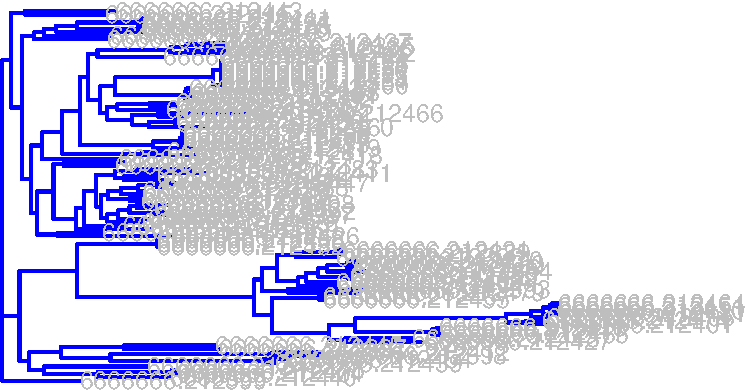
\includegraphics{tesis_files/figure-latex/testingPhylogeny-1} \end{center}
  
  To capture differences on genomes we sort them phylogenetically.
  Phylogenies can be constructed using different paradigms as Parsimony,
  Maximum Likelihood, and Bayesian inference. Short descriptions of the
  main phylogeny methods are included below.
  
  Why is a tree useful \{Book reference\} why trees are useful for?\\
  * Distance methods\\
  * Parsimony * Maximum Likelihood * Mr bayes
  
  General Trees\\
  Actinobacteria Tree, ArchaeaTree, CyanobacteriaTree.
  
  It's easy to create a list. It can be unordered like
  
  To create a sublist, just indent the values a bit (at least four spaces
  or a tab). (Here's one case where indentation is key!)
  
  \begin{enumerate}
  \def\labelenumi{\arabic{enumi}.}
  \tightlist
  \item
    Item 1
  \item
    Item 2
  \item
    Item 3
  
    \begin{itemize}
    \tightlist
    \item
      Item 3a
    \item
      Item 3b
    \end{itemize}
  \end{enumerate}
  
  \subsubsection{Central DB}\label{central-db}
  
  We chose central pathways from
  {[}\protect\hyperlink{ref-barona-gomezux5fwhatux5f2012}{137}{]}\\
  * BBH Best Bidirectional Hits with studied enzymes from Central
  Actinobacterial pathways were selected.
  
  \begin{itemize}
  \item
    By abundance
  \item
    By expansions on genomes
  \end{itemize}
  
  {[}largefiles,\url{https://help.github.com/articles/installing-git-large-file-storage/}{]}
  
  \section{Data Bases}\label{data-bases}
  
  \subsection{Central pathways}\label{central-pathways}
  
  Central database were chosen by BBH from
  
  \begin{Shaded}
  \begin{Highlighting}[]
  \NormalTok{table <-}\StringTok{ }\KeywordTok{read.csv}\NormalTok{(}\StringTok{"chapter1/WC_Central/BBH_Organisms.txt"}\NormalTok{, }\DataTypeTok{row.names =} \DecValTok{1}\NormalTok{,}\DataTypeTok{sep=}\StringTok{"}\CharTok{\textbackslash{}t}\StringTok{"}\NormalTok{)}
  \KeywordTok{kable}\NormalTok{(table,  }\DataTypeTok{caption =} \StringTok{"BBH_Organisms }\CharTok{\textbackslash{}\textbackslash{}}\StringTok{label\{tab:BBH_Organisms\}"}\NormalTok{,}\DataTypeTok{caption.short =} \StringTok{"BBH_Organisms "}\NormalTok{)}
  \end{Highlighting}
  \end{Shaded}
  
  \begin{longtable}[c]{@{}lllll@{}}
  \caption{BBH\_Organisms \label{tab:BBH_Organisms}}\tabularnewline
  \toprule
  & RastId & Database & Taxa1 & Taxa2\tabularnewline
  \midrule
  \endfirsthead
  \toprule
  & RastId & Database & Taxa1 & Taxa2\tabularnewline
  \midrule
  \endhead
  Corynebacterium glutamicum & 6666666.112876 & Actinobacteria &
  &\tabularnewline
  Streptomyces coelicolor A3(2) NC\_003888.3 & & Actinobacteria &
  &\tabularnewline
  Mycobacterium tuberculosis H37Rv NC\_000962.3 & 6666666.146923 &
  Actinobacteria & &\tabularnewline
  Methanosarcina acetivorans C2A AE010299.1 & 6666666.211599 & Archaea &
  Euryarchaeota & Methanomicrobia\tabularnewline
  Nanoarchaeum equitans Kin4-M - AE017199.1 & 6666666.211718 & Archaea &
  DPANN group & Nanoarchaeota\tabularnewline
  Natronomonas pharaonis DSM 2160 & CR936257.1 & 6666666.211909 & Archaea
  & Euryarchaeota\tabularnewline
  Halobacteria & & & &\tabularnewline
  Sulfolobus solfataricus P2 AE006641.1 & 6666666.211567 & Archaea & TACK
  group & Crenarchaeota\tabularnewline
  Cyanothece sp. ATCC 51142 CP000806.1 & 6666666.212444 & Cyanobacteria &
  Oscillatoriales &\tabularnewline
  Synechococcus sp. PCC 7002 CP000951.1 & 6666666.212477 & Cyanobacteria &
  Synechococcales &\tabularnewline
  Arthrospira platensis C1 & 6666666.189647 & Cyanobacteria &
  Cyanobacteria &\tabularnewline
  \bottomrule
  \end{longtable}
  
  \subsection{Genome Dynamics}\label{genome-dynamics}
  
  Among BBH central databases, genomic dynamics was included.\\
  Whats change
  site:\href{http://pubseed.theseed.org/wc.cgi?request=show_otus\&base=/homes/nselem/Data/CS}{WC
  Data}
  
  groups were formed with 100Cyanos, 100Archaea , 118 Actinos Closed,
  43StreptosClosed\\
  Selected organims were
  
  \begin{Shaded}
  \begin{Highlighting}[]
  \NormalTok{table <-}\StringTok{ }\KeywordTok{read.csv}\NormalTok{(}\StringTok{"chapter1/WC_Central/WC_Organisms.txt"}\NormalTok{, }\DataTypeTok{row.names =} \DecValTok{1}\NormalTok{,}\DataTypeTok{sep=}\StringTok{"}\CharTok{\textbackslash{}t}\StringTok{"}\NormalTok{)}
  \KeywordTok{kable}\NormalTok{(table,  }\DataTypeTok{caption =} \StringTok{"WC_Organisms }\CharTok{\textbackslash{}\textbackslash{}}\StringTok{label\{tab:WC_Organisms\}"}\NormalTok{,}\DataTypeTok{caption.short =} \StringTok{"WC_Organisms "}\NormalTok{)}
  \end{Highlighting}
  \end{Shaded}
  
  \begin{longtable}[c]{@{}lrl@{}}
  \caption{WC\_Organisms \label{tab:WC_Organisms}}\tabularnewline
  \toprule
  & Rast.Id & Database\tabularnewline
  \midrule
  \endfirsthead
  \toprule
  & Rast.Id & Database\tabularnewline
  \midrule
  \endhead
  Arthrospira platensis NIES-39 AP011615.1 & 6666666.21 &
  Cyanos\tabularnewline
  Synechococcus sp. PCC 7002 & 6666666.21 & Cyanos\tabularnewline
  Cyanothece sp. ATCC 51142 & 6666666.21 & Cyanos\tabularnewline
  Methanosarcina acetivorans & 6666666.21 & Archaea\tabularnewline
  Nanoarchaeum equitans Kin4-M & 6666666.21 & Archaea\tabularnewline
  Natronomonas pharaonis DSM 2160 & 6666666.21 & Archaea\tabularnewline
  Sulfolobus solfataricus P2 & 6666666.21 & Archaea\tabularnewline
  Mycobacterium tuberculosis H37Rv & 83332.23 & Actinos\tabularnewline
  Corynebacterium glutamicum ATCC 13032 & 196627.31 &
  Actinos\tabularnewline
  Streptomyces coelicolor A3(2) NC\_003888.3 & 6666666.11 & Actinos and
  Streptomyces\tabularnewline
  Streptomyces sp. Mg1 NZ\_CP011664.1 & 6666666.15 &
  Streptomyces\tabularnewline
  \bottomrule
  \end{longtable}
  
  Those families present on at least as much as genomes on the group\\
  Cyanos 100 647\\
  Abundant.Families.100Cyanos\\
  Actinos 118 132\\
  Abundant.Families.43Strepto\\
  Archaea 100 35\\
  Abundant.Families.Actinos\\
  Streptomyces 43 1263\\
  Abundant.Families.Archaeas
  
  Those families expanded on at least two groups\\
  \texttt{cat\ *Abun*\ \textbar{}\ cut\ -f3\textbar{}\ sort\ \textbar{}\ uniq\ -c\ \textbar{}\ sort\ \textgreater{}Abundance.all}\\
  
  Those Families expanded on Archaea and not expanded on Actino\\
  \texttt{comm\ -23\ f3Archaeas\ f3Actinos\ \textgreater{}ArchaeasNoActinos}\\
  Those Families expanded on Actino and not on Archaea\\
  \texttt{comm\ -13\ f3Archaeas\ f3Actinos\ \textgreater{}ActinosNoArchaea}
  
  Those families expanded on Streptomyces but not in ActinoBacteria\\
  \texttt{comm\ -13\ f343Strepto\ f3Actinos\ \textgreater{}ActinosNoStrepto}\\
  Those Families expanded on Actinobacteria and not in Streptomyces\\
  \texttt{comm\ -23\ f343Strepto\ f3Actinos\ \textgreater{}StreptoNoActinos}
  
  Those Families expanded on Cyano and not in Actino\\
  \texttt{comm\ -23\ f3Cyanos\ f3Actinos\ \textgreater{}CyanosNoActinos}
  
  \subsubsection{Natural Products DB}\label{natural-products-db}
  
  Natural products was improved from previous version
  
  \subsection{AntisMASH optional DB}\label{antismash-optional-db}
  
  AntiSMASH is
  {[}\protect\hyperlink{ref-weberux5fantismashux5f2015}{138}{]}\\
  \#\#\# Archaeas Results Archaea is a kingdom of recent discovery were
  not many natural products has been known. On Actinobacteria, evoMining
  has proved its value to find new kinds of natural products. The clue to
  this discovery was that Actinobacteria has genomic expanssions. Now
  Archaea has genomic expansions, even more has central pathways genomic
  expansions. Are this expansions derived from a genomic duplication?\\
  Has Archaea natural products detected by antismash, and if not, where
  are this NP's or may Archaea doesn't have NP's.
  
  applying EvoMining to Archaea
  
  \subsection{Otras estrategias para los clusters Argon context
  Idea}\label{otras-estrategias-para-los-clusters-argon-context-idea}
  
  \section{Argonne}\label{argonne}
  
  ssh
  \href{mailto:nselem@login.mcs.anl.gov}{\nolinkurl{nselem@login.mcs.anl.gov}}\\
  phrase\\
  ssh \href{mailto:nselem@maple}{\nolinkurl{nselem@maple}}\\
  password
  
  cs close strain\\
  wc whats chain
  
  we source (edit bashrc)\\
  link ln (create a link to ross directory)\\
  run out of power:\\
  screen
  
  in Seqs (not mine)\\
  cat\\
  6666666.103569 6666666.112815 6666666.112823 6666666.112833
  6666666.112841 6666666.112849 6666666.112857 \textgreater{}
  /home/nse/Concat\_Full\\
  to find paralogous sets\\
   svr\_representative\_sequences -b -f Id\_Clust -s 0.5 \textless{}
  Concat\_Full \textgreater{} TempFull\&\\
   perl -p -i -e `s/\r//' readable.tree to clean the tree\\
  To find contexts o pegs of paralogous sets
  
  Context midle point 5000 bp (using text tables)\\
  scp 6666666.112839.txt
  \href{mailto:nselem@maple}{\nolinkurl{nselem@maple}}:/homes/nselem/Strepto\_01/.
  
  fig\textbar{}6666666.112839.peg.26
  
  copy families.all file\\
  on the file we have column1 family name column 5 peg id
  
  cluster\_objects \textless{} elements\_to\_cluster \textgreater{}
  ClusteFile
  
  write a file with pegs\\
  1 peg1 adjacent1, adjacent2 \ldots{}.\\
  1 peg2\\
  2\\
  2
  
  write a file similiar but with the family number
  
  1 peg1 fn1, fn2 \ldots{}.\\
  1 peg2\\
  2\\
  2
  
  compare each peg on this file from the same family
  
  Write the conextions file\\
  peg1 peg2\\
  peg1 peg3\\
  peg2 peg3
  
  cluster this file and score the cluster
  
  Define
  
  \begin{verbatim}
  1.  a "function set" is generated by the what's changed directory  
  \end{verbatim}
  
  as a ``family''
  
  \begin{verbatim}
  2.  a "paralog set" is a set of function sets in which paralogous  
  \end{verbatim}
  
  members span the sets
  
  \begin{verbatim}
  3.  a PEG is in a paralog set if it is in one ofthe function sets  
  \end{verbatim}
  
  that make up the
  
  \begin{verbatim}
  4.  a "context" of a PEG is the set of close pegs  
  4.1 First cluster operation would give us: context sets  (CS)  
  
  5.  a "context set" is a set of PEGs with "similar contexts"  
  5.1 second clustering operation would give us:cluster  (Cl)  
  
  6.  a "cluster" is a set of context sets (each context set is a different   
  \end{verbatim}
  
  compute:\\
   Compute the context sets that are made from PEGs that occur in PS.\\
   Compute the contexts of PEGs in PS.
  
  cluster these context using the ``similar contexts'' relation
  
  This gives a set of clusters, and the members of the clusters are
  context sets\\
  That is, a cluster is a set of context sets
  
  \begin{verbatim}
    a. the number of contexts sets i  
  \end{verbatim}
  
  score the clusters\\
   Take a paralog set PS.\\
   Be the context sets: CS\_1, CS\_2,\ldots{}, CS\_k members of the
  paralogous set\\
   k the number of contexts sets on the paralogous set\\
   n\_i the cardinality of CS\_i
  
  \begin{verbatim}
  PS={CS1,CS2,...,CS3}  
  Cl={[CS_1,n_1],[CS_2,n_2],...,[CS_k,n_k]}  
  
  let be M=max(n_i)   i=1,2,..k (Maximum cardinality of Context sets)  
      m=max(n_i)   i=1,2,..k, i!=M (second greatest cardinality of context sets)  
      (We are intersted that a second copy is distributed)  
  
  We are interested on k,M,n to form a scoring function for the cluster set  
  S=f(k,m,M)=c_1*k+c_2*m+c_3*M  
  \end{verbatim}
  
  history
  
  Para hacer un nuevo set de datos
  
  591 cd Data/CS\\
   592 mkdir Directorio\\
   593 vi Directorio/rep.genomes\\
   594 cd Directorio/\\
   600 nohup svr\_CS -d Directorio\&
  
  Contenido de rep.genomes\\
  rast\textbar{}390693 nselem35 q8Vf6ib\\
  rast\textbar{}390675 nselem35 q8Vf6ib\\
  rast\textbar{}388811 nselem35 q8Vf6ib
  
  When you click the \textbf{Knit} button above a document will be
  generated that includes both content as well as the output of any
  embedded \textbf{R} code chunks within the document. You can embed an
  \textbf{R} code chunk like this (\texttt{cars} is a built-in \textbf{R}
  dataset):
  
  \begin{Shaded}
  \begin{Highlighting}[]
  \KeywordTok{summary}\NormalTok{(cars)}
  \end{Highlighting}
  \end{Shaded}
  
  \begin{verbatim}
       speed           dist       
   Min.   : 4.0   Min.   :  2.00  
   1st Qu.:12.0   1st Qu.: 26.00  
   Median :15.0   Median : 36.00  
   Mean   :15.4   Mean   : 42.98  
   3rd Qu.:19.0   3rd Qu.: 56.00  
   Max.   :25.0   Max.   :120.00  
  \end{verbatim}
  
  \subsection{Inline code}\label{inline-code}
  
  If you'd like to put the results of your analysis directly into your
  discussion, add inline code like this:
  
  \begin{quote}
  The \texttt{cos} of \(2 \pi\) is 1.
  \end{quote}
  
  Another example would be the direct calculation of the standard
  deviation:
  
  \begin{quote}
  The standard deviation of \texttt{speed} in \texttt{cars} is 5.2876444.
  \end{quote}
  
  One last neat feature is the use of the \texttt{ifelse} conditional
  statement which can be used to output text depending on the result of an
  \textbf{R} calculation:
  
  \begin{quote}
  The standard deviation is less than 6.
  \end{quote}
  
  Note the use of \texttt{\textgreater{}} here, which signifies a
  quotation environment that will be indented.
  
  As you see with \texttt{\$2\ \textbackslash{}pi\$} above, mathematics
  can be added by surrounding the mathematical text with dollar signs.
  More examples of this are in {[}Mathematics and Science{]} if you
  uncomment the code in {[}Math{]}.
  
  \section{Recomendaciones de Luis}\label{recomendaciones-de-luis}
  
  Para evoMining\\
  Probar distintos métodos de filogenia y después hacer la coloración.\\
  maximum likelihood, Protest phyml\\
  Atracción de ramas largas.\\
  raxml\\
  trim all vs Gblocs (Tony Galvadon)
  
  Comparar dos árboles\\
  Para ver si la evolución de los genes concatenados ha sido simultánea\\
  Robinson and foulds\\
  Joe Felsestein\\
  Phylip
  
  \begin{enumerate}
  \def\labelenumi{\arabic{enumi}.}
  \setcounter{enumi}{1}
  \tightlist
  \item
    dist tree\\
    quarter descomposition\\
    peter gogarten fendou Mao
  \end{enumerate}
  
  Sets de experimentos.\\
  Para el experimento de los streptomyces con ruta centrales el core,
  analizar el problema de dominios múltiples.\\
  Dominios\\
  Nan Song, Dannie durand\\
  Después del blast
  
  Para obtener\\
  Pablo Vinuesa: Get Homologues
  
  Burkhordelias y su toxina (Preguntar a Beto)\\
  Cianobacterias y la ruta de fijación de nitrógeno.
  
  Servidor Viernes a las 12:00
  
  \section{CORASON: Other genome Mining tools
  context-based}\label{corason-other-genome-mining-tools-context-based}
  
  \section{CORe Analysis of Syntenic Orthologs to prioritize Natural
  Product-Biosynthetic Gene
  Cluster}\label{core-analysis-of-syntenic-orthologs-to-prioritize-natural-product-biosynthetic-gene-cluster}
  
  Genome fluidity on Bacteria is source of biosynthetic gene clusters
  (BGCs) abundance, in fact almost all bacterial genome sequenced
  contributes with new genes and gene clusters to the Bacterial Pangenome.
  As a consequence of gene diversity helped by sequence technology
  advances, researchers often have a large set of genomes that wish to
  analize in search of a particular gene cluster variation. Answering BGCs
  analysis needs CORASON allows users to find and visualice variations of
  a given gene cluster sorting them according to the conserved core
  phylogeny.
  
  To find cluster variations, given a query protein sequence that belongs
  to a reference cluster, CORASON will search on a Bacterial genome
  database all gene clusters that contains orthologues of the
  query-protein and at least another sequence from the reference cluster.
  Orthologues on variation clusters are coloured within a gradient
  according to its identity percentage with the reference cluster
  sequences.
  
  The cluster core attempts to identify a set of functions conserved on
  this particular biosynthetic BGC. The core genome on a taxonomical group
  is the set of coding sequences that are shared between all group
  members, this definition may be adapted to the cluster core by using a
  set of gene clusters instead of a set of genomes. A report about gene
  function will be provided whenever a cluster core exists also core
  sequences will be concatenated to construct a phylogenetic tree and sort
  variation clusters accordingly.
  
  Functional annotations are provided by RAST annotation service due to
  that CORASON genomic databases must be RAST files. Any archaeal or
  bacterial genome can be RAST annotated either on the website or by
  command line using myrast server.
  
  Finally, in order to provide an easy to install distribution CORASON was
  packaged on docker containerization platform. Software dependencies such
  as BLAST 2.2.30, muscle3.8.3, GBlocksLinux64\_0.91b, quicktree,
  newick-utils-1.6, and CORASON code were wrapped together on CORASON
  docker container.
  \href{https://github.com/nselem/EvoDivMet/wiki}{Tutorial} and software
  are available at nselem/github.
  
  CORASON inputs are a genomic database, a reference cluster and an enzyme
  inside this cluster, outputs are newick trees, core functional report
  and a cluster variation SVG file. SVG format among being high quality
  scalable graphics, also allow to display metadata such as gene function
  and genome coordinates just by mouse over figures on a browser
  facilitating genomic analysis.
  
  In conclusion CORASON is an easy to install comparative genomic visual
  tool on a customizable genome database that allows users to visualice
  variations of a reference gene cluster identifing its core functions and
  finally sorting variations according to their evolutionary history
  helping to prioritize clusters that may be involved on chemical novelty.
  
  You can also embed plots. For example, here is a way to use the base
  \textbf{R} graphics package to produce a plot using the built-in
  \texttt{pressure} dataset:
  
  \begin{center}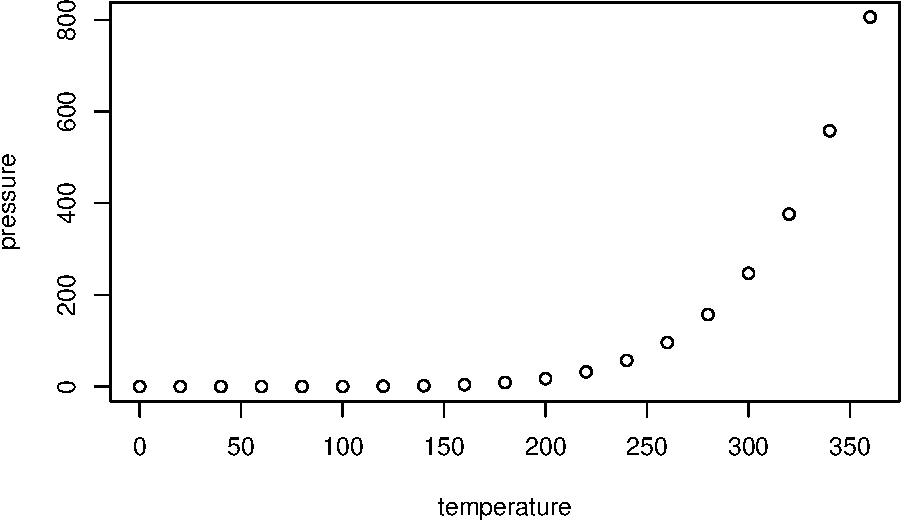
\includegraphics{tesis_files/figure-latex/pressure-1} \end{center}
  
  Note that the \texttt{echo\ =\ FALSE} parameter was added to the code
  chunk to prevent printing of the \textbf{R} code that generated the
  plot. There are plenty of other ways to add chunk options. More
  information is available at \url{http://yihui.name/knitr/options/}.
  
  Another useful chunk option is the setting of \texttt{cache\ =\ TRUE} as
  you see here. If document rendering becomes time consuming due to long
  computations or plots that are expensive to generate you can use knitr
  caching to improve performance. Later in this file, you'll see a way to
  reference plots created in \textbf{R} or external figures.
  
  \section{Loading and exploring data}\label{loading-and-exploring-data}
  
  Included in this template is a file called \texttt{flights.csv}. This
  file includes a subset of the larger dataset of information about all
  flights that departed from Seattle and Portland in 2014. More
  information about this dataset and its \textbf{R} package is available
  at \url{http://github.com/ismayc/pnwflights14}. This subset includes
  only Portland flights and only rows that were complete with no missing
  values. Merges were also done with the \texttt{airports} and
  \texttt{airlines} data sets in the \texttt{pnwflights14} package to get
  more descriptive airport and airline names.
  
  We can load in this data set using the following command:
  
  \begin{Shaded}
  \begin{Highlighting}[]
  \NormalTok{flights <-}\StringTok{ }\KeywordTok{read.csv}\NormalTok{(}\StringTok{"data/flights.csv"}\NormalTok{)}
  \end{Highlighting}
  \end{Shaded}
  
  The data is now stored in the data frame called \texttt{flights} in
  \textbf{R}. To get a better feel for the variables included in this
  dataset we can use a variety of functions. Here we can see the
  dimensions (rows by columns) and also the names of the columns.
  
  \begin{Shaded}
  \begin{Highlighting}[]
  \KeywordTok{dim}\NormalTok{(flights)}
  \end{Highlighting}
  \end{Shaded}
  
  \begin{verbatim}
  [1] 52808    16
  \end{verbatim}
  
  \begin{Shaded}
  \begin{Highlighting}[]
  \KeywordTok{names}\NormalTok{(flights)}
  \end{Highlighting}
  \end{Shaded}
  
  \begin{verbatim}
   [1] "month"        "day"          "dep_time"     "dep_delay"   
   [5] "arr_time"     "arr_delay"    "carrier"      "tailnum"     
   [9] "flight"       "dest"         "air_time"     "distance"    
  [13] "hour"         "minute"       "carrier_name" "dest_name"   
  \end{verbatim}
  
  Another good idea is to take a look at the dataset in table form. With
  this dataset having more than 50,000 rows, we won't explicitly show the
  results of the command here. I recommend you enter the command into the
  Console \textbf{\emph{after}} you have run the \textbf{R} chunks above
  to load the data into \textbf{R}.
  
  \begin{Shaded}
  \begin{Highlighting}[]
  \KeywordTok{View}\NormalTok{(flights)}
  \end{Highlighting}
  \end{Shaded}
  
  While not required, it is highly recommended you use the \texttt{dplyr}
  package to manipulate and summarize your data set as needed. It uses a
  syntax that is easy to understand using chaining operations. Below I've
  created a few examples of using \texttt{dplyr} to get information about
  the Portland flights in 2014. You will also see the use of the
  \texttt{ggplot2} package, which produces beautiful, high-quality
  academic visuals.
  
  We begin by checking to ensure that needed packages are installed and
  then we load them into our current working environment:
  
  The example we show here does the following:
  
  \begin{itemize}
  \item
    Selects only the \texttt{carrier\_name} and \texttt{arr\_delay} from
    the \texttt{flights} dataset and then assigns this subset to a new
    variable called \texttt{flights2}.
  \item
    Using \texttt{flights2}, we determine the largest arrival delay for
    each of the carriers.
  \end{itemize}
  
  \begin{Shaded}
  \begin{Highlighting}[]
  \NormalTok{flights2 <-}\StringTok{ }\NormalTok{flights %>%}\StringTok{ }\NormalTok{dplyr::}\KeywordTok{select}\NormalTok{(carrier_name, arr_delay)}
  \NormalTok{max_delays <-}\StringTok{ }\NormalTok{flights2 %>%}\StringTok{ }\KeywordTok{group_by}\NormalTok{(carrier_name) %>%}
  \StringTok{  }\KeywordTok{summarize}\NormalTok{(}\DataTypeTok{max_arr_delay =} \KeywordTok{max}\NormalTok{(arr_delay, }\DataTypeTok{na.rm =} \OtherTok{TRUE}\NormalTok{))}
  \end{Highlighting}
  \end{Shaded}
  
  We next introduce a useful function in the \texttt{knitr} package for
  making nice tables in \emph{R Markdown} called \texttt{kable}. It
  produces the \LaTeX~code required to make the table and is much easier
  to use than manually entering values into a table by copying and pasting
  values into Excel or \LaTeX. This again goes to show how nice
  reproducible documents can be! There is no need to copy-and-paste values
  to create a table. (Note the use of \texttt{results\ =\ "asis"} here
  which will produce the table instead of the code to create the table.
  You'll learn more about the
  \texttt{\textbackslash{}\textbackslash{}label} later.) The
  \texttt{caption.short} argument is used to include a shorter version of
  the title to appear in the List of Tables at the beginning of the
  document.
  
  \begin{Shaded}
  \begin{Highlighting}[]
  \KeywordTok{kable}\NormalTok{(max_delays, }\DataTypeTok{col.names =} \KeywordTok{c}\NormalTok{(}\StringTok{"Airline"}\NormalTok{, }\StringTok{"Max Arrival Delay"}\NormalTok{),}
        \DataTypeTok{caption =} \StringTok{"Maximum Delays by Airline }\CharTok{\textbackslash{}\textbackslash{}}\StringTok{label\{tab:max_delay\}"}\NormalTok{,}
        \DataTypeTok{caption.short =} \StringTok{"Max Delays by Airline"}\NormalTok{)}
  \end{Highlighting}
  \end{Shaded}
  
  \begin{longtable}[c]{@{}lr@{}}
  \caption{Maximum Delays by Airline \label{tab:max_delay}}\tabularnewline
  \toprule
  Airline & Max Arrival Delay\tabularnewline
  \midrule
  \endfirsthead
  \toprule
  Airline & Max Arrival Delay\tabularnewline
  \midrule
  \endhead
  Alaska Airlines Inc. & 338\tabularnewline
  American Airlines Inc. & 1539\tabularnewline
  Delta Air Lines Inc. & 651\tabularnewline
  Frontier Airlines Inc. & 575\tabularnewline
  Hawaiian Airlines Inc. & 407\tabularnewline
  JetBlue Airways & 273\tabularnewline
  SkyWest Airlines Inc. & 421\tabularnewline
  Southwest Airlines Co. & 694\tabularnewline
  United Air Lines Inc. & 472\tabularnewline
  US Airways Inc. & 347\tabularnewline
  Virgin America & 366\tabularnewline
  \bottomrule
  \end{longtable}
  
  We can further look into the properties of the largest value here for
  American Airlines Inc. To do so, we can isolate the row corresponding to
  the arrival delay of 1539 minutes for American in our original
  \texttt{flights} dataset.
  
  \begin{Shaded}
  \begin{Highlighting}[]
  \NormalTok{flights %>%}\StringTok{ }\NormalTok{dplyr::}\KeywordTok{filter}\NormalTok{(arr_delay ==}\StringTok{ }\DecValTok{1539}\NormalTok{, }
                     \NormalTok{carrier_name ==}\StringTok{ "American Airlines Inc."}\NormalTok{) %>%}
  \StringTok{  }\NormalTok{dplyr::}\KeywordTok{select}\NormalTok{(-}\KeywordTok{c}\NormalTok{(month, day, carrier, dest_name, hour, }
              \NormalTok{minute, carrier_name, arr_delay))}
  \end{Highlighting}
  \end{Shaded}
  
  \begin{verbatim}
    dep_time dep_delay arr_time tailnum flight dest air_time distance
  1     1403      1553     1934  N595AA   1568  DFW      182     1616
  \end{verbatim}
  
  We see that the flight occurred on March 3rd and departed a little after
  2 PM on its way to Dallas/Fort Worth. Lastly, we show how we can
  visualize the arrival delay of all departing flights from Portland on
  March 3rd against time of departure.
  
  \begin{Shaded}
  \begin{Highlighting}[]
  \NormalTok{flights %>%}\StringTok{ }\NormalTok{dplyr::}\KeywordTok{filter}\NormalTok{(month ==}\StringTok{ }\DecValTok{3}\NormalTok{, day ==}\StringTok{ }\DecValTok{3}\NormalTok{) %>%}
  \StringTok{  }\KeywordTok{ggplot}\NormalTok{(}\KeywordTok{aes}\NormalTok{(}\DataTypeTok{x =} \NormalTok{dep_time, }\DataTypeTok{y =} \NormalTok{arr_delay)) +}
  \StringTok{  }\KeywordTok{geom_point}\NormalTok{()}
  \end{Highlighting}
  \end{Shaded}
  
  \begin{center}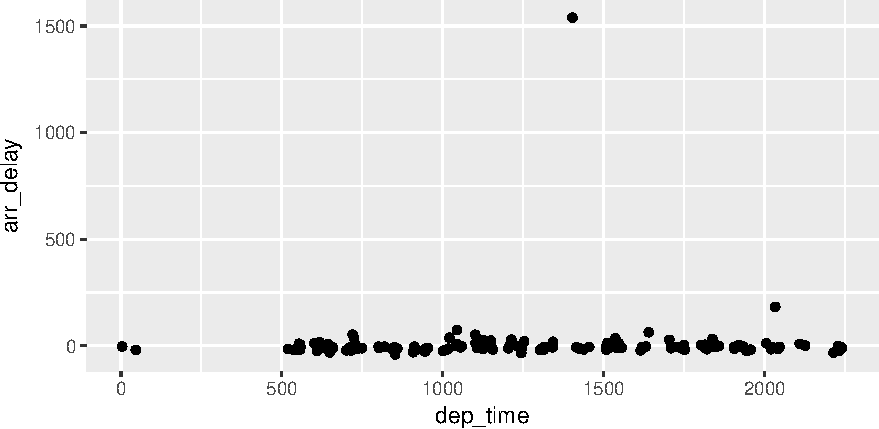
\includegraphics{tesis_files/figure-latex/march3plot-1} \end{center}
  
  \chapter{PriA Family}\label{math-sci}
  
  PriA is an homologous of HisA,\\
  on Actinobacteria phylum, TrpF is gene lost.
  
  PriA is a promiscuous enzyme family involved in histidine and triptophan
  pathways performing HisA and TrpF functions respectibly. This enzyme
  family catalizes convertions converting ProFAR into PRFAR acting as a
  HisA and isomerizes PRA into CdRP acting as TrpF.
  
  PriA shows a functional gradient on Actinobacteria that dicide this
  family into enzymatic subfamilies. Between PriA subfamilies there is
  PriB family on Streptomyces with little trpF activity, subHisA on
  Corynebacteria and Actinomyces, subTrpF on Actinomyces,
  
  \clearpage  
  
  \section{Enzymes}\label{enzymes}
  
  39 Streptomyces PriA sequence 39 Streptomyces sequences, as outgroup E
  coli, Arthrobacter Aurescens, Salmonella enterica and Acidimicrobium
  ferrooxidans PriA's were included.
  
  as an outgroup with HisA activity Enterobacterias \emph{Salmonella
  enterica} (PDB:5AHE), \emph{Escherichia coli K12} \emph{Acidimicrobium
  ferrooxydans} (PDB:4WD0) Additionally to the sequences selected by
  phylogeny, Jonesia denitrificans and Streptomyces sp Mg1 TrpF sequences
  were added as control .
  
  PriA\\
  \emph{Mycobacterium tuberculosis} (Mtub PDB:2Y88,2Y89,2Y85,3ZS4)
  \emph{Streptomyces coelicolor} (Scoe
  PDB:2VEP,2X30,1VZW),\emph{Streptomyces globisporus}, \emph{Actynomyces
  urogenitalis} 4X2R \emph{Corynebacterium jeikeum}
  
  subHisA\\
  \emph{Corynebacterium diphteriae} \emph{Actinomyces car} (PDB:4X2R)
  
  subTrpF\\
  \emph{Arthrobacter aurescens} (PDB:4WD0)
  
  PriB\\
  \emph{Streptomyces ipomoeae}, \emph{Streptomyces sviceus}
  (PDB:4U28,4TX9)\\
  TrpF controls \emph{Jonesia denitrificans} (PDB:4WUI) \emph{Chlamidya
  thrachomatis}, \emph{Streptomyces sp. Mg1} TrpF and \emph{Actinomyces
  odontolyticus} were included
  
  Streptomyces 34 paralogous
  
  \section{CORASON}\label{corason}
  
  PriA All streptomyces have a partially conserved PriA cluster. CT34 has
  a secondary copy whose Best hit on NCBI is Lentzea's PriA with 50\%
  identity 98\% coverage
  
  TrpF1 TrpF1 queries gave hits with TrpC enzyme present on every
  Streptomyces, additionally S rimosus, S coelicolor, S venezuelae and S.
  NRRL S-1813 had an extra copy. S rimosus TrpC vicinity has PKS and
  siderophore genes.
  
  TrpF2 Conserved cluster with NRPS sequences flanking TrpF2
  
  TrpF3 Non conserved cluster
  
  TrpF4 purpeofuscus and S bikiniensis 2. Heatmap
  
  \clearpage  
  
  \section{Structures}\label{structures}
  
  \begin{Shaded}
  \begin{Highlighting}[]
  \NormalTok{table <-}\StringTok{ }\KeywordTok{read.csv}\NormalTok{(}\StringTok{"chapter2/EstructurasPDB"}\NormalTok{, }\DataTypeTok{row.names =} \DecValTok{1}\NormalTok{,}\DataTypeTok{sep=}\StringTok{"}\CharTok{\textbackslash{}t}\StringTok{"}\NormalTok{)}
  \KeywordTok{kable}\NormalTok{(table,  }\DataTypeTok{caption =} \StringTok{"Enzyme PDB }\CharTok{\textbackslash{}\textbackslash{}}\StringTok{label\{tab:Enzyme PDB\}"}\NormalTok{,}\DataTypeTok{caption.short =} \StringTok{"Enzyme PDB "}\NormalTok{)}
  \end{Highlighting}
  \end{Shaded}
  
  \begin{longtable}[c]{@{}llllrr@{}}
  \caption{Enzyme PDB \label{tab:Enzyme PDB}}\tabularnewline
  \toprule
  & Organismo & Family & Observations & Resolution & Year\tabularnewline
  \midrule
  \endfirsthead
  \toprule
  & Organismo & Family & Observations & Resolution & Year\tabularnewline
  \midrule
  \endhead
  4WUI & Jonesia denitrificans & TrpF & & 1.09 & 2014\tabularnewline
  4X9S & Streptomyces sp. MG1 & PriB & & 1.60 & 2014\tabularnewline
  5DN1 & Streptomyces coelicolor & PriA & & 1.95 & 2015\tabularnewline
  1DL3 & Thermotoga maritima & TrpF & & 2.70 & 1999\tabularnewline
  1LBM & Thermotoga maritima & TrpF & RCDRP & 2.80 & 2002\tabularnewline
  1NSJ & Thermotoga maritima & TrpF & & 2.00 & 1996\tabularnewline
  1V5X & Thermus thermophilus & TrpF & & 2.00 & 2003\tabularnewline
  1VZW & Streptomyces coelicolor & PriA & & 1.80 & 2004\tabularnewline
  2VEP & Streptomyces coelicolor & PriA & & 1.80 & 2007\tabularnewline
  2X30 & Streptomyces coelicolor & PriA & R139N & 1.95 &
  2010\tabularnewline
  2Y85 & Mycobacterium tuberculosis & PriA & RCDRP & 2.40 &
  2011\tabularnewline
  2Y88 & Mycobacterium tuberculosis & PriA & D11N PRFAR & 1.33 &
  2011\tabularnewline
  2Y89 & Mycobacterium tuberculosis & PriA & D11N & 2.50 &
  2011\tabularnewline
  3ZS4 & Mycobacterium tuberculosis & PriA & PRFAR & 1.90 &
  2012\tabularnewline
  4AAJ & Pyrococcus furiosus & TrpF & & 1.75 & 2012\tabularnewline
  4TX9 & Streptomyces sviceus & PriB & ProFAR & 1.60 & 2014\tabularnewline
  4U28 & Streptomyces sviceus & PriB & & 1.33 & 2014\tabularnewline
  4W9T & Streptomyces sp. Mg1 & PriB & & 1.57 & 2014\tabularnewline
  4WD0 & Arthrobacter aurescens & PriB & & 1.50 & 2014\tabularnewline
  4X2R & Actinomyces urogenitalis & & & 1.05 & 2014\tabularnewline
  4AXK & Corynebacterium efficiens & SubHisA & & 2.25 &
  2013\tabularnewline
  5AHE & Salmonella enterica & HisA & & 1.70 & 2015\tabularnewline
  5AB3 & Salmonella enterica & HisA & D7N, D10G, dup13-15, Q24L, G102A &
  1.80 & 2016\tabularnewline
  5ABT & Salmonella enterica & HisA & D7N, G102A, V106M, D176A & 1.65 &
  2016\tabularnewline
  5AC7 & Salmonella enterica & HisA & D7N, D10G, dup13-15 & 1.90 &
  2016\tabularnewline
  5AC8 & Salmonella enterica & HisA & D10G, dup13-15, G102A & 1.70 &
  2016\tabularnewline
  5AC6 & Salmonella enterica & HisA & D7N, D10G, dup13-15, Q24L, G102A &
  1.99 & 2016\tabularnewline
  5A5W & Salmonella enterica & HisA & HisA D7N D176A with ProFAR & NA &
  2015\tabularnewline
  5AHF & Salmonella enterica & HisA & HisA D7N with ProFAR & NA &
  NA\tabularnewline
  4GJ1 & Campylobacter jejuni & HisA & & 2.15 & 2012\tabularnewline
  2W79 & Thermotoga maritima & HisA & & 1.85 & 2008\tabularnewline
  1QO2 & Thermotoga maritima & HisA & & 1.85 & 2000\tabularnewline
  5LHE & Thermococcus kodakaraensis & TrpF & & 1.85 & 2016\tabularnewline
  5LHF & Thermococcus kodakaraensis & TrpF & & 1.75 & 2016\tabularnewline
  \bottomrule
  \end{longtable}
  
  \clearpage 
  \#\# Substrates\\
  20 substrates were collected from literature and chemioinformatics
  predictions.\\
  S13,S14,!5,S16 light activated substrates, S3 PRA, S7 PROFAR, S6 GMP,
  S11 GTP, S17 PRAP, S18 Compound V, S17 PraP
  
  \begin{Shaded}
  \begin{Highlighting}[]
  \NormalTok{table <-}\StringTok{ }\KeywordTok{read.csv}\NormalTok{(}\StringTok{"chapter2/Substrate.data"}\NormalTok{, }\DataTypeTok{row.names =} \DecValTok{1}\NormalTok{,}\DataTypeTok{sep=}\StringTok{"}\CharTok{\textbackslash{}t}\StringTok{"}\NormalTok{)}
  \KeywordTok{kable}\NormalTok{(table,  }\DataTypeTok{caption =} \StringTok{"Substrates }\CharTok{\textbackslash{}\textbackslash{}}\StringTok{label\{tab:substrates\}"}\NormalTok{,}\DataTypeTok{caption.short =} \StringTok{"Substrates "}\NormalTok{)}
  \end{Highlighting}
  \end{Shaded}
  
  \begin{longtable}[c]{@{}lllllll@{}}
  \caption{Substrates \label{tab:substrates}}\tabularnewline
  \toprule
  & id & Number & Kind & Reference & Names & Observations\tabularnewline
  \midrule
  \endfirsthead
  \toprule
  & id & Number & Kind & Reference & Names & Observations\tabularnewline
  \midrule
  \endhead
  S13 & dte6\_open & LUZ & & & & NA\tabularnewline
  S15 & dte13\_open & LUZ & & & & NA\tabularnewline
  S14 & dte6\_closed & LUZ & & & & NA\tabularnewline
  S16 & dte13\_closed & LUZ & & & & NA\tabularnewline
  S10 & C04376 & & James & & 5'-Phosphoribosyl-N-formylglycinamide &
  NA\tabularnewline
  S12 & C03838 & & James & & 5'-Phosphoribosylglycinamide &
  NA\tabularnewline
  S9 & C04640 & & James & &
  2-(Formamido)-N1-(5'-phosphoribosyl)acetamidine & NA\tabularnewline
  S18 & CompoundV & & Adams & CompundV & This compound is an intermediary
  between GTP and H2NMP & NA\tabularnewline
  S5 & C05923 & & James & & 2,5-Diaminopyrimidine nucleoside triphosphate
  & NA\tabularnewline
  S4 & C05922 & & James & & Formamidopyrimidine nucleoside triphosphate &
  NA\tabularnewline
  S8 & C01268 & & James & & 5-Amino-6-(5'-phosphoribosylamino)uracil &
  NA\tabularnewline
  S17 & PraP & & Verduzco & PraP & & NA\tabularnewline
  S7 & C04302 & & James & & PRA & NA\tabularnewline
  S6 & C00144 & & James & & GMP & NA\tabularnewline
  S11 & C00044 & & James & & GTP & NA\tabularnewline
  S1 & C01253 & & James & & ADP-D-ribosyl-{[}dinitrogen reductase{]} &
  NA\tabularnewline
  S2 & C01201 & & James & & N(omega)-(ADP-D-ribosyl)-L-arginine &
  NA\tabularnewline
  S3 & C04896 & & & & ProFAR & NA\tabularnewline
  S19 & S\_17146 & & Due et al & 17146 &
  2,5-dimethyl-N-(4-oxocyclohexa-2,5-dienylidene)benzenesulfonamide
  \#17146, 4456-2380, Chem-Div & NA\tabularnewline
  S20 & S\_16827 & & Due et al & 16827 &
  (E)-N-(3-chloro-5-methyl-4-oxocyclohexa-2,5-dienylidene)
  benzenesulfonamide, \#16827, 3993-4586, Chem-Div & NA\tabularnewline
  \bottomrule
  \end{longtable}
  
  \begin{figure}[h!tbp]
   \centering
   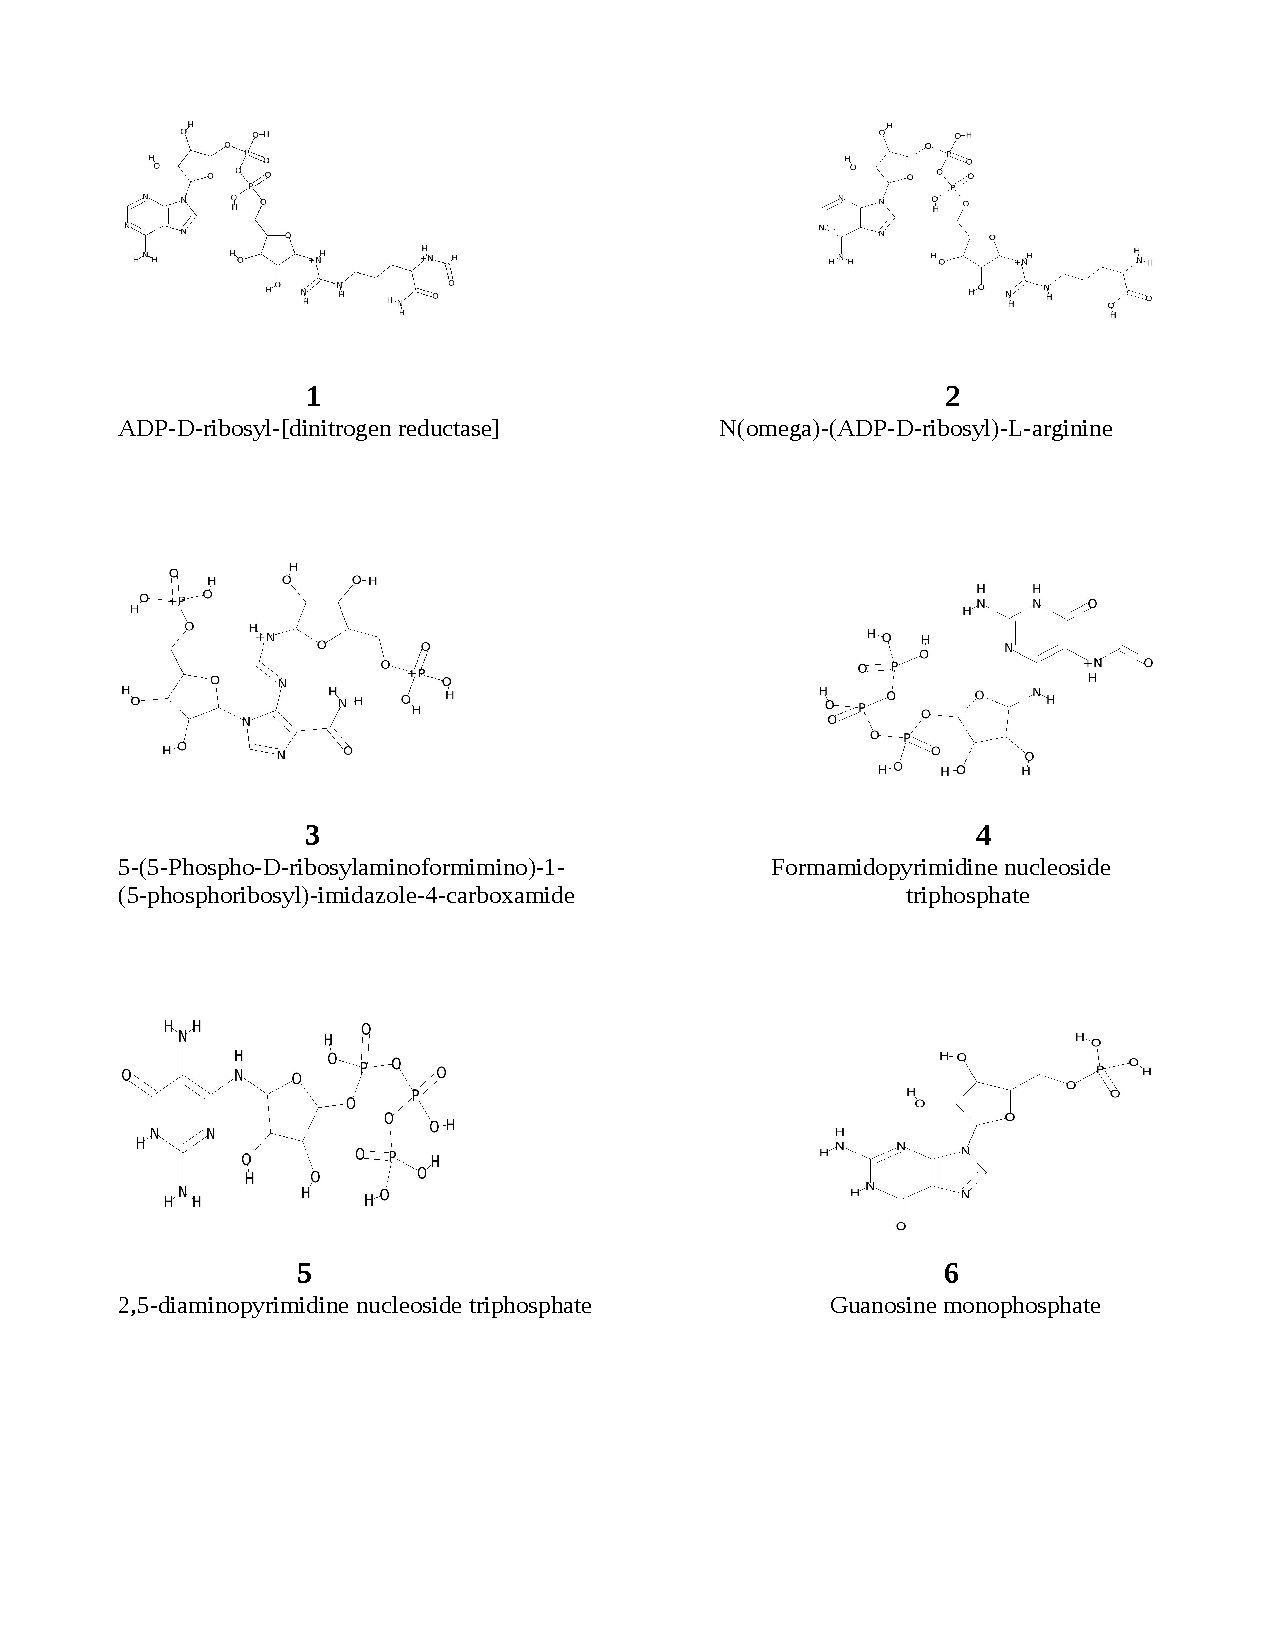
\includegraphics[angle = 0,scale = 1]{chapter2/esquema_quimico-1-1.pdf}
   \caption[Substrates 1]{\normalsize{Substrates 1}}
   \label{fig:Substrates chemical 1}
   \end{figure}
  
  \begin{figure}[h!tbp]
   \centering
   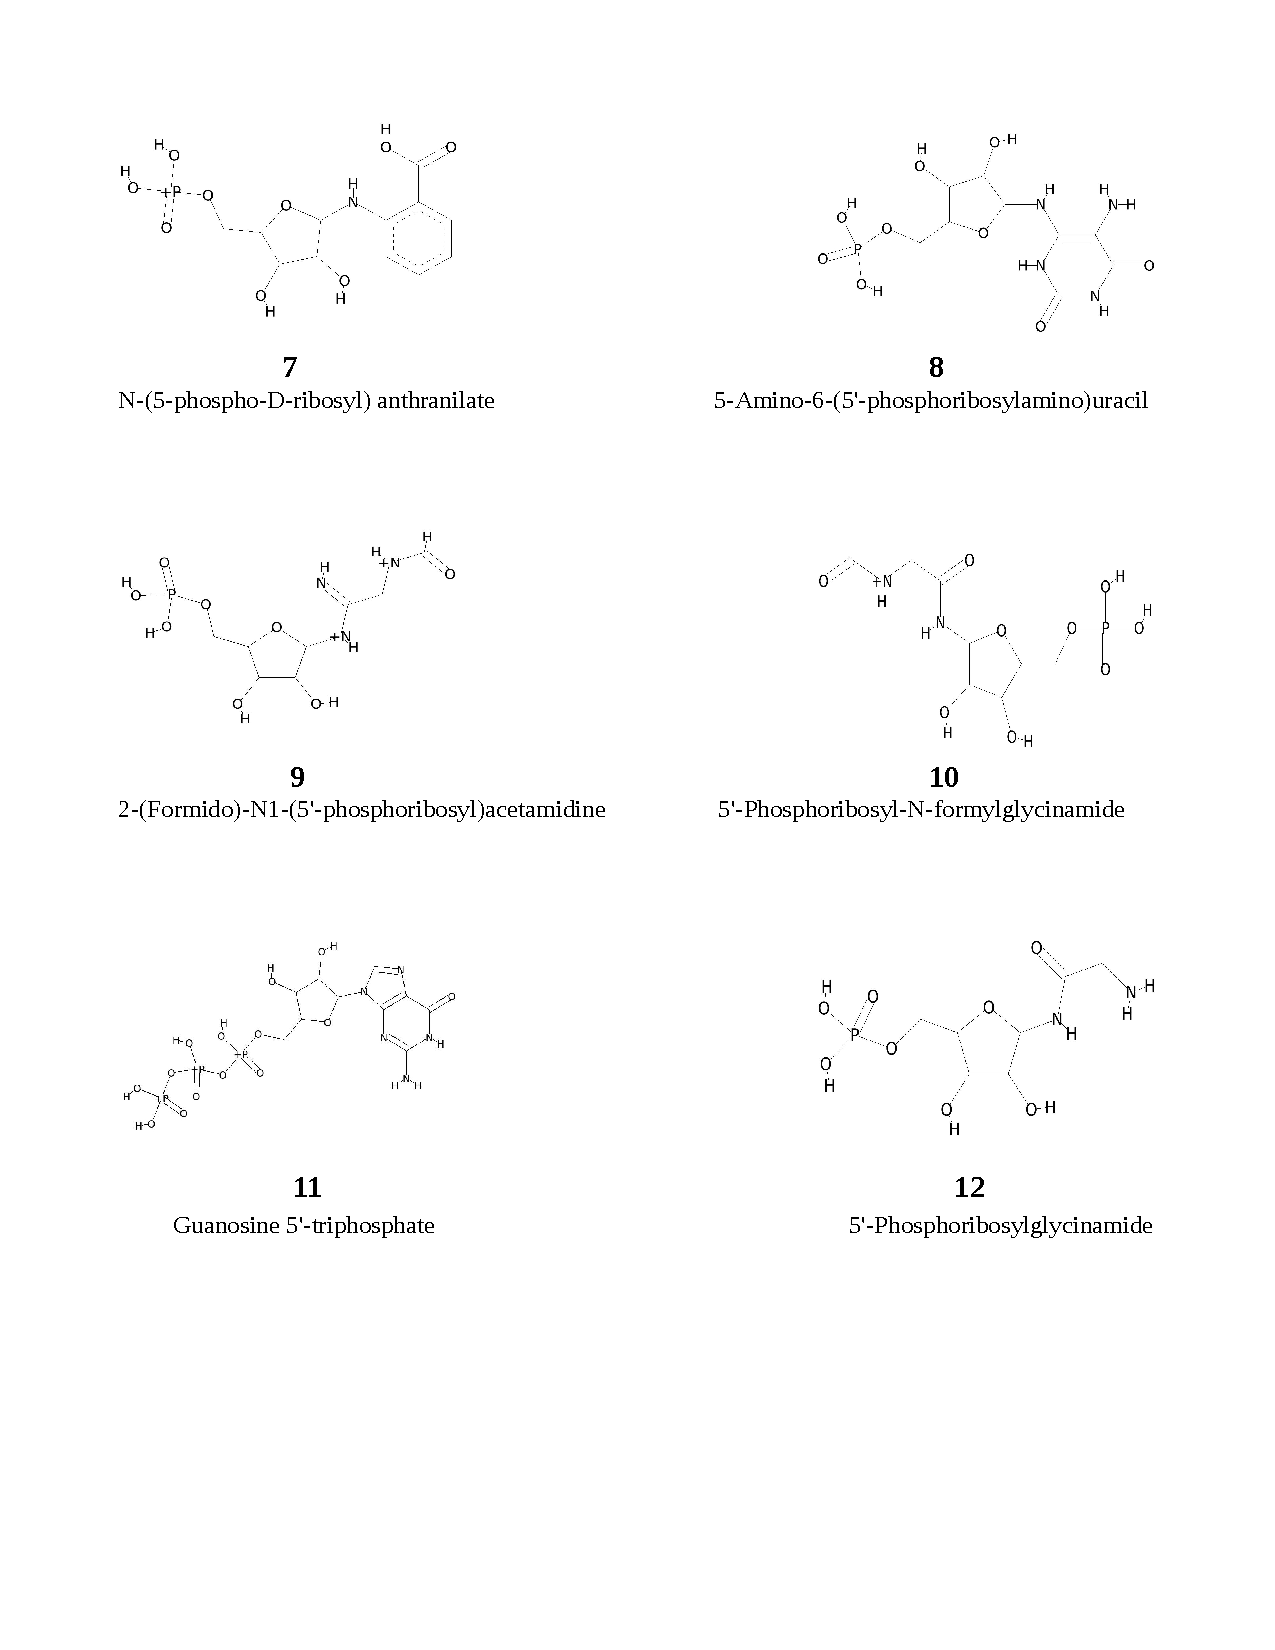
\includegraphics[angle = 0,scale = 1]{chapter2/esquema_quimico-2-2.pdf}
   \caption[Substrates 2]{\normalsize{Substrates 2}}
   \label{fig:Substrates chemical 2}
   \end{figure}
  
  \begin{figure}[h!tbp]
   \centering
   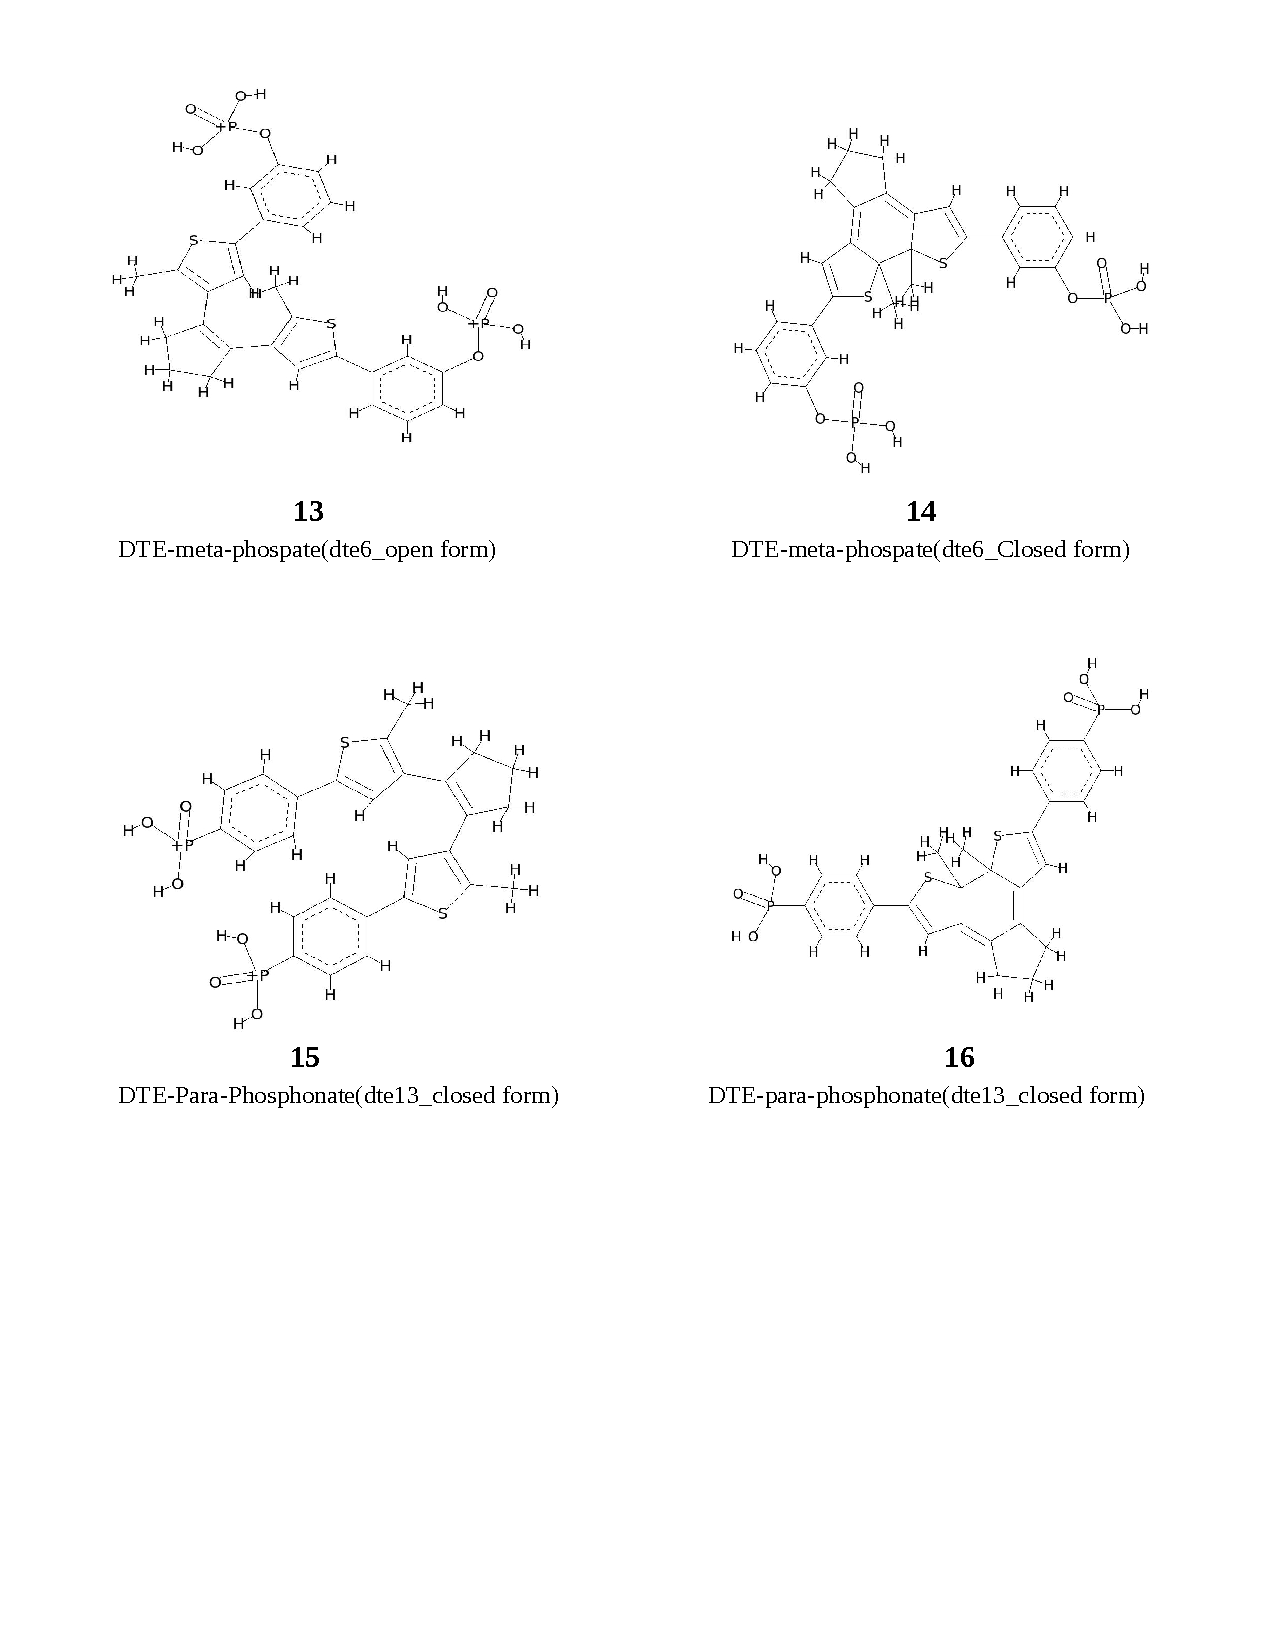
\includegraphics[angle = 0,scale = 1]{chapter2/esquema_quimico-3-3.pdf}
   \caption[Substrates 3]{\normalsize{Substrates 3}}
   \label{fig:Substrates chemical 3}
   \end{figure}
  
  \begin{figure}[h!tbp]
   \centering
   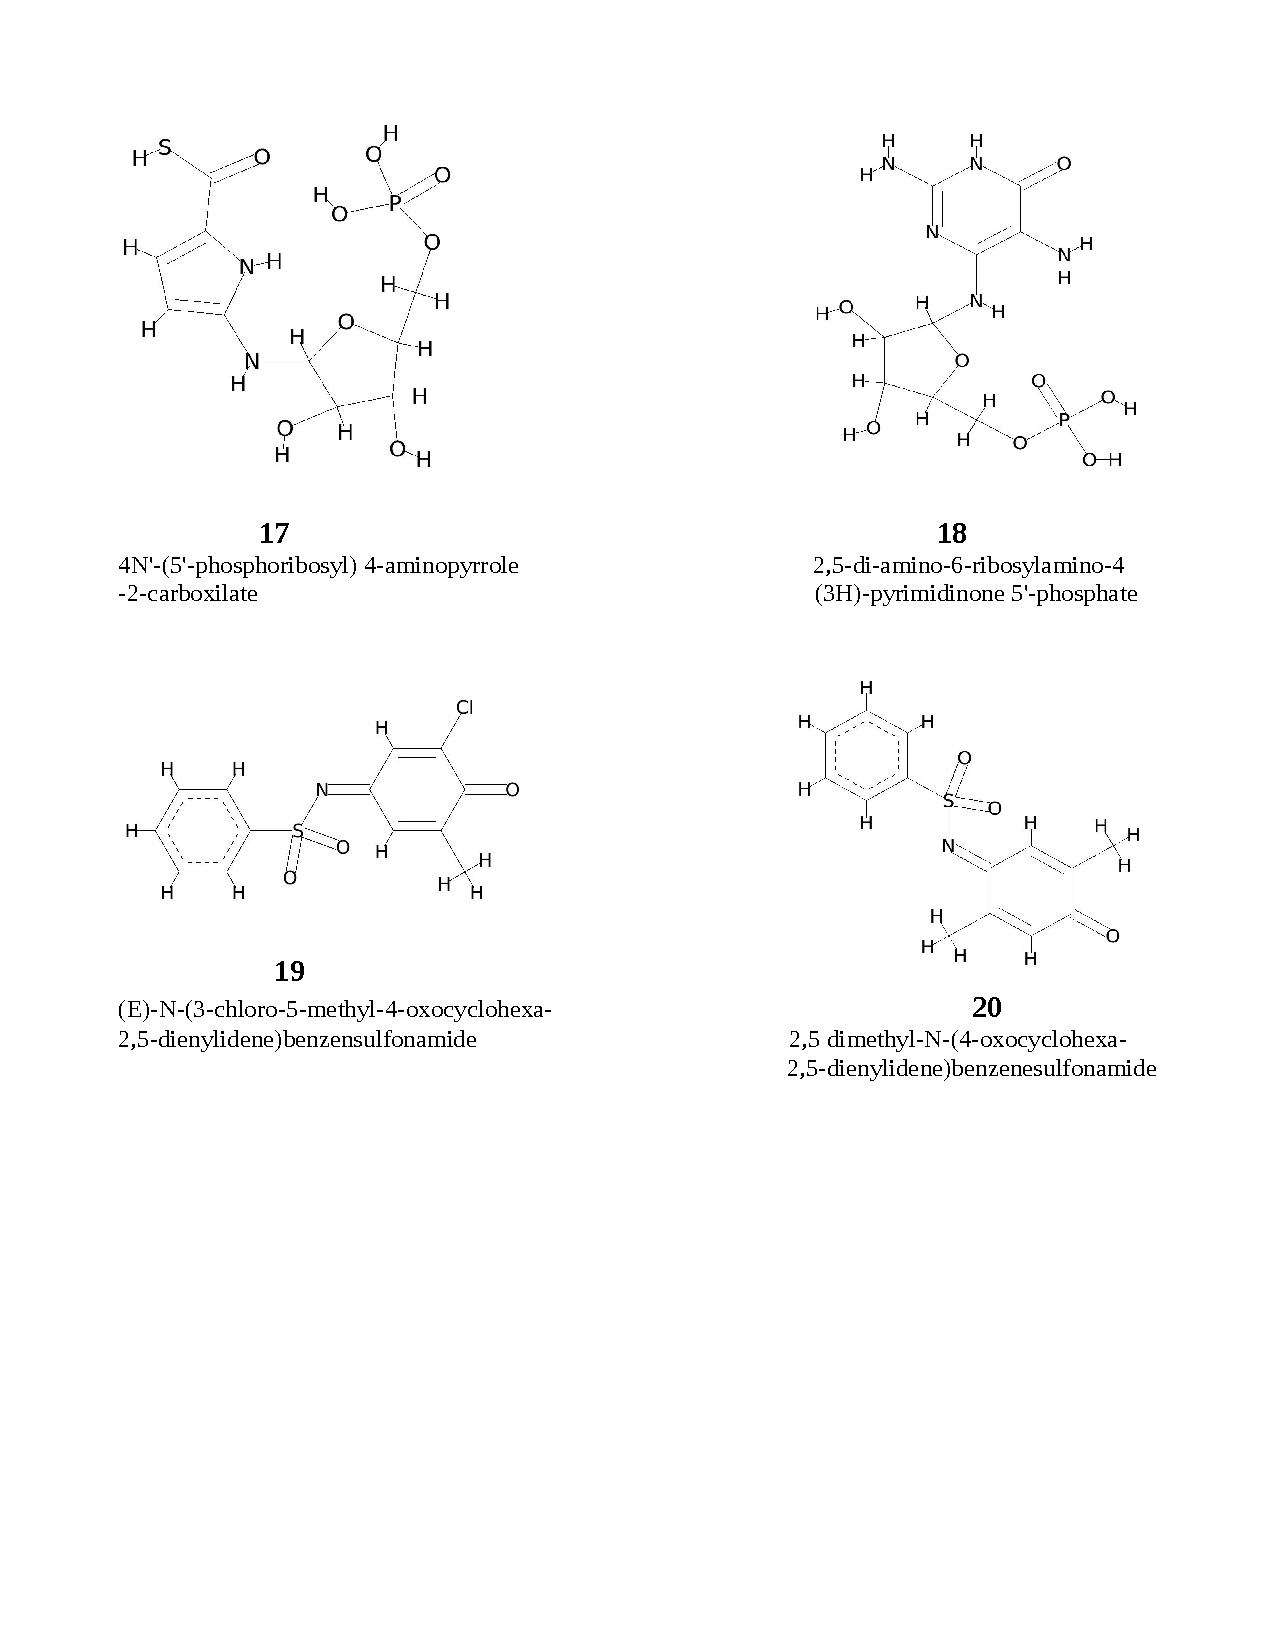
\includegraphics[angle = 0,scale = 1]{chapter2/esquema_quimico-4-4.pdf}
   \caption[Substrates 4]{\normalsize{Substrates 4}}
   \label{fig:Substrates chemical 4}
   \end{figure}
  
  \section{Docking}\label{docking}
  
  Docking simulation were calculated for PriA Streptomyces enzymes. TrpF
  enzymes from Strptomyces Mg1, Jonesia denitrificans, were added as
  controls
  
  Procedures can be found at
  \href{https://github.com/tripplab/Docking/wiki}{Docking Protocols}
  
  \clearpage 
  
  \begin{Shaded}
  \begin{Highlighting}[]
  \NormalTok{docking <-}\StringTok{ }\KeywordTok{read.csv}\NormalTok{(}\StringTok{"chapter2/SmallHeat.data"}\NormalTok{, }\DataTypeTok{header=}\OtherTok{TRUE}\NormalTok{, }\DataTypeTok{sep=}\StringTok{"}\CharTok{\textbackslash{}t}\StringTok{"}\NormalTok{)}
  \KeywordTok{kable}\NormalTok{(docking,  }\DataTypeTok{caption =} \StringTok{"Enzymes docking }\CharTok{\textbackslash{}\textbackslash{}}\StringTok{label\{tab:docking\}"}\NormalTok{,}\DataTypeTok{caption.short =} \StringTok{"Enzymes docking "}\NormalTok{)}
  \end{Highlighting}
  \end{Shaded}
  
  \begin{longtable}[c]{@{}lrrrrrrrrrrrrrrrrrrrr@{}}
  \caption{Enzymes docking \label{tab:docking}}\tabularnewline
  \toprule
  Enzima & S13 & S15 & S14 & S16 & S10 & S12 & S9 & S18 & S5 & S4 & S8 &
  S17 & S7 & S6 & S11 & S1 & S2 & S3 & S19 & S20\tabularnewline
  \midrule
  \endfirsthead
  \toprule
  Enzima & S13 & S15 & S14 & S16 & S10 & S12 & S9 & S18 & S5 & S4 & S8 &
  S17 & S7 & S6 & S11 & S1 & S2 & S3 & S19 & S20\tabularnewline
  \midrule
  \endhead
  Srub\_2VEP & -7.4 & -7.3 & -7.5 & -7.1 & -6.5 & -6.2 & -6.5 & -7.7 &
  -9.4 & -9.3 & -7.9 & -7.2 & -8.3 & -8.6 & -8.9 & -9.0 & -7.1 & -8.9 &
  -7.8 & -7.7\tabularnewline
  Saver\_2VEP & -7.4 & -7.2 & -7.0 & -6.5 & -7.3 & -6.4 & -7.0 & -7.5 &
  -9.6 & -8.5 & -7.9 & -7.6 & -8.4 & -8.7 & -9.8 & -8.3 & -7.9 & -8.6 &
  -7.7 & -7.6\tabularnewline
  Scoe\_2VEP & -7.5 & -7.5 & -7.9 & -7.0 & -7.0 & -6.2 & -6.5 & -7.8 &
  -8.8 & -9.2 & -7.8 & -7.9 & -8.0 & -8.9 & -10.3 & -9.2 & -9.3 & -8.4 &
  -8.1 & -8.2\tabularnewline
  Scoe\_2X30 & -8.1 & -7.4 & -7.6 & -6.9 & -6.7 & -6.8 & -7.1 & -7.9 &
  -9.1 & -9.0 & -8.3 & -8.6 & -8.5 & -9.0 & -10.6 & -10.0 & -10.3 & -10.2
  & -8.1 & -7.9\tabularnewline
  Scoe\_1VZW & NA & NA & NA & NA & NA & NA & NA & NA & NA & NA & NA & NA &
  NA & NA & NA & NA & NA & NA & NA & NA\tabularnewline
  Sfla\_2VEP & -7.1 & -7.6 & -7.2 & -7.3 & -7.2 & -6.8 & -6.9 & -8.1 &
  -8.2 & -7.2 & -8.2 & -7.2 & -8.4 & -8.3 & -8.5 & -7.9 & -7.8 & -6.0 &
  -7.5 & -7.3\tabularnewline
  Sgha\_2VEP & -9.2 & -8.7 & -6.7 & -6.7 & -7.4 & -7.7 & -7.2 & -7.5 &
  -9.8 & -8.9 & -8.2 & -7.8 & -8.8 & -8.7 & -10.1 & -9.1 & -9.0 & -9.5 &
  -8.0 & -7.5\tabularnewline
  Siak\_2VEP & -6.6 & -7.3 & -7.0 & -7.1 & -7.1 & -7.1 & -6.8 & -8.0 &
  -9.2 & -8.7 & -7.8 & -7.6 & -8.3 & -8.4 & -9.1 & -5.8 & -5.3 & -8.5 &
  -7.3 & -7.4\tabularnewline
  Sbic\_2VEP & -7.2 & -6.7 & -6.8 & -6.5 & -6.2 & -6.6 & -5.9 & -7.8 &
  -8.5 & -7.8 & -7.8 & -7.2 & -8.2 & -8.0 & -9.6 & -8.2 & -8.0 & -9.4 &
  -7.7 & -7.5\tabularnewline
  Sbot\_2VEP & -9.6 & -10.9 & -8.9 & -7.1 & -6.0 & -6.2 & -6.7 & -8.1 &
  -9.1 & -8.8 & -8.3 & -7.9 & -8.9 & -9.3 & -9.4 & -9.8 & -10.0 & -8.9 &
  -8.2 & -8.0\tabularnewline
  Sipo\_2VEP & -6.6 & -6.6 & -7.3 & -6.9 & -6.5 & -6.3 & -6.5 & -8.1 &
  -8.6 & -9.1 & -8.0 & -7.9 & -8.0 & -8.4 & -8.5 & -7.2 & -8.4 & -8.2 &
  -7.9 & -7.6\tabularnewline
  Ssvi & NA & NA & NA & NA & NA & NA & NA & NA & NA & NA & NA & NA & NA &
  NA & NA & NA & NA & NA & NA & NA\tabularnewline
  Ssvi\_4U28 & NA & NA & NA & NA & NA & NA & NA & NA & NA & NA & NA & NA &
  NA & NA & NA & NA & NA & NA & NA & NA\tabularnewline
  Ssvi\_4TX9 & -5.9 & -8.2 & -7.1 & -6.6 & -6.8 & -7.0 & -7.6 & -7.9 &
  -8.4 & -8.3 & -8.2 & -8.1 & -8.4 & -8.7 & -7.7 & -8.2 & -8.2 & -6.7 &
  -8.0 & -7.5\tabularnewline
  Salb\_2VEP & -6.3 & -7.1 & -7.4 & -6.8 & -7.7 & -6.9 & -6.6 & -8.0 &
  -9.6 & -8.9 & -8.6 & -7.9 & -8.6 & -8.4 & -9.1 & -7.4 & -7.2 & -8.8 &
  -8.1 & -7.8\tabularnewline
  Sbik\_2VEP & -7.4 & -6.7 & -7.4 & -7.3 & -7.7 & -6.5 & -6.8 & -8.5 &
  -9.9 & -9.8 & -8.3 & -7.8 & -8.2 & -8.4 & -10.5 & -7.1 & -6.3 & -8.3 &
  -8.1 & -7.9\tabularnewline
  Stsu\_2VEP & -6.9 & -7.5 & -7.9 & -7.8 & -7.5 & -7.3 & -7.7 & -8.1 &
  -10.0 & -9.7 & -8.7 & -7.8 & -8.8 & -8.8 & -10.6 & -7.8 & -8.7 & -9.2 &
  -7.9 & -7.8\tabularnewline
  Sven\_2VEP & -8.3 & -7.6 & -7.5 & -6.8 & -6.4 & -7.0 & -6.2 & -8.2 &
  -9.6 & -9.0 & -7.9 & -7.4 & -8.3 & -8.6 & -10.0 & -8.2 & -8.2 & -8.1 &
  -7.6 & -7.4\tabularnewline
  Scal\_2VEP & -7.3 & -8.8 & -7.5 & -6.7 & -7.0 & -6.5 & -6.5 & -8.7 &
  -10.0 & -9.7 & -8.8 & -7.7 & -8.2 & -8.6 & -10.5 & -8.1 & -9.2 & -8.9 &
  -7.6 & -7.6\tabularnewline
  Sbaa\_2VEP & -8.9 & -6.6 & -6.7 & -6.8 & -7.2 & -7.2 & -6.2 & -7.7 &
  -9.6 & -9.5 & -8.4 & -7.4 & -8.5 & -8.2 & -9.7 & -8.5 & -8.4 & -9.3 &
  -7.4 & -7.7\tabularnewline
  Sglo\_2VEP & -6.1 & -6.8 & -6.9 & -6.5 & -6.7 & -6.3 & -6.7 & -7.5 &
  -9.6 & -9.6 & -8.6 & -7.8 & -8.7 & -8.7 & -9.9 & -6.2 & -5.1 & -9.2 &
  -7.8 & -7.7\tabularnewline
  Sful\_2VEP & -9.0 & -6.9 & -7.1 & -6.8 & -6.3 & -7.2 & -6.6 & -8.1 &
  -9.8 & -9.3 & -7.7 & -8.0 & -8.7 & -8.8 & -10.5 & -7.6 & -9.1 & -10.5 &
  -7.1 & -7.4\tabularnewline
  Sgri\_2VEP & -6.6 & -8.2 & -7.1 & -6.4 & -7.1 & -7.4 & -7.1 & -7.4 &
  -9.4 & -8.5 & -8.6 & -7.5 & -8.8 & -8.4 & -9.6 & -8.8 & -8.8 & -8.7 &
  -7.7 & -7.5\tabularnewline
  S34\_2VEP & -7.8 & -7.2 & -7.6 & -7.3 & -6.2 & -6.5 & -6.9 & -8.0 & -8.8
  & -8.6 & -7.7 & -7.1 & -7.7 & -7.9 & -7.2 & -7.1 & -6.7 & -7.1 & -7.7 &
  -7.7\tabularnewline
  Srim\_2VEP & -7.4 & -6.8 & -7.1 & -7.2 & -7.2 & -7.4 & -7.8 & -8.6 &
  -9.7 & -9.3 & -8.8 & -7.7 & -8.9 & -8.7 & -10.2 & -6.8 & -8.2 & -9.0 &
  -7.5 & -7.8\tabularnewline
  Satr\_2VEP & -7.6 & -7.1 & -7.5 & -7.4 & -6.2 & -6.5 & -6.9 & -8.0 &
  -8.9 & -8.7 & -7.7 & -7.4 & -7.7 & -7.8 & -6.5 & -7.0 & -6.3 & -7.7 &
  -7.7 & -7.7\tabularnewline
  S1813\_2VEP & -7.5 & -6.7 & -6.8 & -6.6 & -6.8 & -7.0 & -6.7 & -7.9 &
  -9.9 & -9.7 & -8.3 & -7.7 & -8.5 & -8.6 & -10.0 & -7.6 & -7.5 & -8.6 &
  -7.3 & -7.5\tabularnewline
  Svar\_2VEP & -6.3 & -6.8 & -7.0 & -6.3 & -6.9 & -6.9 & -6.6 & -7.8 &
  -9.3 & -7.4 & -8.5 & -7.3 & -8.0 & -8.7 & -8.5 & -7.4 & -6.3 & -6.0 &
  -7.9 & -7.5\tabularnewline
  Sfra\_2VEP & -7.3 & -7.0 & -6.8 & -6.6 & -6.5 & -7.3 & -6.6 & -8.6 &
  -9.1 & -8.7 & -8.9 & -7.7 & -8.9 & -9.0 & -8.7 & -6.0 & -6.3 & -7.9 &
  -8.2 & -7.8\tabularnewline
  Smeg\_2VEP & -8.0 & -7.3 & -6.9 & -6.6 & -7.2 & -6.7 & -6.1 & -7.6 &
  -9.2 & -9.1 & -7.8 & -7.4 & -8.2 & -8.5 & -9.6 & -9.2 & -9.2 & -8.6 &
  -7.7 & -7.5\tabularnewline
  Ssul\_2VEP & -7.5 & -7.0 & -6.9 & -6.6 & -6.6 & -6.7 & -6.9 & -7.7 &
  -8.4 & -8.2 & -8.2 & -7.5 & -8.1 & -7.7 & -8.2 & -6.7 & -7.1 & -7.7 &
  -7.6 & -7.4\tabularnewline
  Slav\_4X9S & -8.0 & -7.1 & -6.7 & -6.9 & -6.6 & -6.8 & -6.7 & -8.2 &
  -9.5 & -9.1 & -8.6 & -8.0 & -8.4 & -8.7 & -9.1 & -9.5 & -9.3 & -8.1 &
  -8.1 & -7.6\tabularnewline
  Sery\_4X9S & -7.8 & -7.2 & -7.6 & -7.2 & -7.4 & -6.9 & -7.4 & -8.5 &
  -9.4 & -9.4 & -8.6 & -7.6 & -8.4 & -8.6 & -9.1 & -10.0 & -10.1 & -9.0 &
  -7.8 & -8.2\tabularnewline
  SspC\_4X9S & -7.4 & -6.9 & -7.3 & -6.8 & -7.3 & -6.6 & -7.5 & -8.0 &
  -9.8 & -9.3 & -8.7 & -7.6 & -8.5 & -8.4 & -10.6 & -9.1 & -8.9 & -8.5 &
  -8.1 & -8.0\tabularnewline
  Sxan\_4X9S & -7.5 & -6.9 & -6.8 & -6.8 & -6.5 & -6.6 & -6.5 & -8.3 &
  -8.0 & -8.1 & -7.6 & -7.4 & -8.7 & -8.1 & -8.1 & -8.5 & -8.0 & -7.6 &
  -7.7 & -7.4\tabularnewline
  Skat\_4X9S & -6.4 & -7.0 & -7.1 & -6.7 & -7.7 & -6.3 & -6.2 & -8.1 &
  -8.5 & -9.2 & -8.3 & -7.6 & -9.0 & -8.5 & -9.7 & -9.5 & -9.9 & -9.2 &
  -7.4 & -7.5\tabularnewline
  SMg1\_4X9S & -6.5 & -6.9 & -7.2 & -7.1 & -6.5 & -6.9 & -6.4 & -7.3 &
  -7.8 & -7.7 & -8.3 & -7.5 & -7.9 & -8.4 & -9.5 & -7.6 & -5.2 & -7.5 &
  -7.6 & -7.7\tabularnewline
  SMg1\_W9T & NA & NA & NA & NA & NA & NA & NA & NA & NA & NA & NA & NA &
  NA & NA & NA & NA & NA & NA & NA & NA\tabularnewline
  Sniv\_2VEP & -6.2 & -6.8 & -7.4 & -6.5 & -7.8 & -6.8 & -6.7 & -9.5 &
  -9.6 & -9.4 & -8.7 & -8.2 & -8.6 & -9.1 & -9.9 & -5.4 & -5.5 & -9.2 &
  -8.0 & -7.5\tabularnewline
  Scla\_2VEP & -6.4 & -7.7 & -7.4 & -7.2 & -7.6 & -7.5 & -7.2 & -8.5 &
  -10.1 & -10.0 & -8.7 & -7.9 & -8.8 & -9.1 & -10.2 & -6.9 & -8.1 & -8.5 &
  -7.7 & -7.7\tabularnewline
  Save\_2VEP & -7.6 & -6.7 & -7.1 & -7.2 & -7.1 & -6.5 & -6.6 & -7.8 &
  -8.6 & -10.0 & -8.6 & -7.5 & -8.3 & -8.5 & -8.8 & -5.3 & -5.2 & -5.8 &
  -7.7 & -7.4\tabularnewline
  Spur\_2vEP & -6.8 & -7.3 & -6.9 & -6.7 & -8.0 & -7.9 & -7.7 & -8.5 &
  -9.5 & -9.8 & -8.1 & -7.8 & -8.7 & -9.7 & -10.0 & -5.3 & -6.2 & -8.2 &
  -7.6 & -7.4\tabularnewline
  Scar\_2Y89 & -6.9 & -6.8 & -7.5 & -7.1 & -7.8 & -7.3 & -7.2 & -8.3 &
  -9.2 & -8.3 & -8.9 & -8.4 & -8.9 & -9.3 & -9.4 & -5.3 & -5.2 & -7.1 &
  -8.5 & -8.6\tabularnewline
  Mtub\_2Y88 & -10.0 & -7.8 & -8.9 & -5.4 & -8.6 & -7.3 & -7.8 & -9.5 &
  -10.9 & -10.3 & -9.5 & -9.0 & -9.8 & -9.8 & -11.3 & -10.1 & -10.2 &
  -11.3 & -9.5 & -8.8\tabularnewline
  Mtub\_2Y89 & -8.7 & -8.6 & -9.6 & -9.4 & -6.4 & -5.9 & -5.6 & -7.1 &
  -7.0 & -7.5 & -7.3 & -6.8 & -7.4 & -8.4 & -7.5 & -8.1 & -8.6 & -7.5 &
  -7.7 & -7.3\tabularnewline
  Mtub\_2Y85 & -8.2 & -7.9 & -9.2 & -7.4 & -7.6 & -7.5 & -7.6 & -8.4 &
  -9.7 & -9.5 & -9.3 & -7.8 & -8.6 & -8.6 & -10.2 & -9.8 & -9.9 & -10.1 &
  -7.3 & -7.4\tabularnewline
  Mtub\_3ZS4 & -10.0 & -10.5 & -11.4 & -6.4 & -8.2 & -7.2 & -7.0 & -9.6 &
  -10.2 & -10.2 & -9.9 & -8.5 & -9.3 & -9.6 & -10.9 & -10.0 & -10.7 & -9.9
  & -8.8 & -8.9\tabularnewline
  S34\_3ZS4 & -7.4 & -8.0 & -7.6 & -6.4 & -5.2 & -5.4 & -5.2 & -6.1 & -6.8
  & -6.4 & -5.7 & -6.4 & -6.3 & -6.3 & -7.1 & -7.4 & -7.1 & -6.4 & -7.1 &
  -6.6\tabularnewline
  Cdip\_4AXK & -9.2 & -7.8 & -10.9 & -7.2 & -7.5 & -7.6 & -7.7 & -8.9 &
  -9.0 & -9.8 & -9.0 & -8.3 & -8.8 & -9.2 & -10.1 & -9.5 & -9.9 & -9.2 &
  -8.0 & -7.9\tabularnewline
  Cjei\_4AXK & -7.5 & -6.9 & -7.2 & -6.5 & -8.4 & -8.0 & -8.5 & -8.7 &
  -9.5 & -9.6 & -9.4 & -8.8 & -9.0 & -9.5 & -9.3 & -8.1 & -9.3 & -8.5 &
  -7.9 & -7.7\tabularnewline
  Aaur & NA & NA & NA & NA & NA & NA & NA & NA & NA & NA & NA & NA & NA &
  NA & NA & NA & NA & NA & NA & NA\tabularnewline
  Aaur\_4WD0 & -8.2 & -8.5 & -8.1 & -7.9 & -5.7 & -5.5 & -5.9 & -7.0 &
  -7.5 & -7.2 & -7.1 & -6.7 & -7.1 & -7.4 & -8.4 & -7.2 & -7.3 & -7.4 &
  -7.0 & -6.7\tabularnewline
  Acar\_4X2R & -10.6 & -9.3 & -9.3 & -7.2 & -7.2 & -6.8 & -7.3 & -7.5 &
  -9.5 & -9.8 & -8.0 & -7.8 & -9.3 & -8.9 & -10.3 & -9.6 & -9.4 & -9.4 &
  -8.1 & -8.0\tabularnewline
  Auro\_4X2R & -9.9 & -9.1 & -9.8 & -8.1 & -7.4 & -7.1 & -7.4 & -7.8 &
  -9.2 & -9.8 & -8.3 & -7.8 & -9.3 & -9.0 & -9.9 & -9.0 & -8.6 & -9.2 &
  -8.5 & -8.2\tabularnewline
  Afer\_4WD0 & -5.7 & -5.8 & -6.0 & -5.7 & -6.7 & -6.2 & -5.8 & -7.6 &
  -9.2 & -8.8 & -7.8 & -7.4 & -8.3 & -8.4 & -9.3 & -6.7 & -4.5 & -9.1 &
  -8.3 & -8.1\tabularnewline
  Sent\_5AHE & -9.1 & -5.4 & -6.4 & -5.2 & -8.0 & -7.3 & -7.4 & -8.8 &
  -10.7 & -10.2 & -8.7 & -8.7 & -9.6 & -9.9 & -10.9 & -7.8 & -9.1 & -10.3
  & -9.0 & -8.4\tabularnewline
  Ecoli\_K12 & -9.7 & -9.7 & -9.2 & -6.1 & -7.2 & -6.6 & -6.8 & -8.6 &
  -9.5 & -9.1 & -8.6 & -8.2 & -9.0 & -8.6 & -10.2 & -9.9 & -10.2 & -9.9 &
  -8.2 & -7.9\tabularnewline
  Jden\_4WUI & -8.3 & -8.8 & -8.2 & -6.8 & -6.2 & -6.1 & -6.0 & -6.8 &
  -7.4 & -7.6 & -7.5 & -6.9 & -7.6 & -7.5 & -7.7 & -7.5 & -7.6 & -7.2 &
  -7.3 & -7.2\tabularnewline
  Ctra & -8.2 & -8.0 & -7.4 & -7.2 & -6.1 & -5.5 & -5.4 & -6.5 & -7.1 &
  -7.1 & -7.0 & -6.2 & -6.8 & -6.8 & -6.9 & -7.2 & -7.4 & -6.5 & -6.7 &
  -6.6\tabularnewline
  SMg1\_trpF & -7.2 & -8.8 & -8.2 & -7.3 & -6.2 & -5.7 & -5.7 & -6.9 &
  -6.6 & -6.7 & -7.3 & -6.7 & -7.6 & -6.9 & -7.5 & -7.1 & -7.1 & -6.9 &
  -6.7 & -6.5\tabularnewline
  Aodo\_4X2R & -8.5 & -8.6 & -8.8 & -7.3 & -7.1 & -7.1 & -7.1 & -7.5 &
  -9.7 & -9.4 & -7.8 & -7.6 & -9.6 & -8.8 & -10.1 & -8.4 & -8.9 & -9.4 &
  -8.0 & -8.1\tabularnewline
  \clearpage & & & & & & & & & & & & & & & & & & & &\tabularnewline
  \bottomrule
  \end{longtable}
  
  \begin{center}\includegraphics{tesis_files/figure-latex/load_data_docking-1} \end{center}
  
  \begin{center}\includegraphics{tesis_files/figure-latex/load_data_docking-2} \end{center}
  
  \begin{verbatim}
  Warning: Removed 100 rows containing non-finite values (stat_boxplot).
  \end{verbatim}
  
  \begin{center}\includegraphics{tesis_files/figure-latex/load_data_docking-3} \end{center}
  
  \begin{figure}[h!tbp]
   \centering
   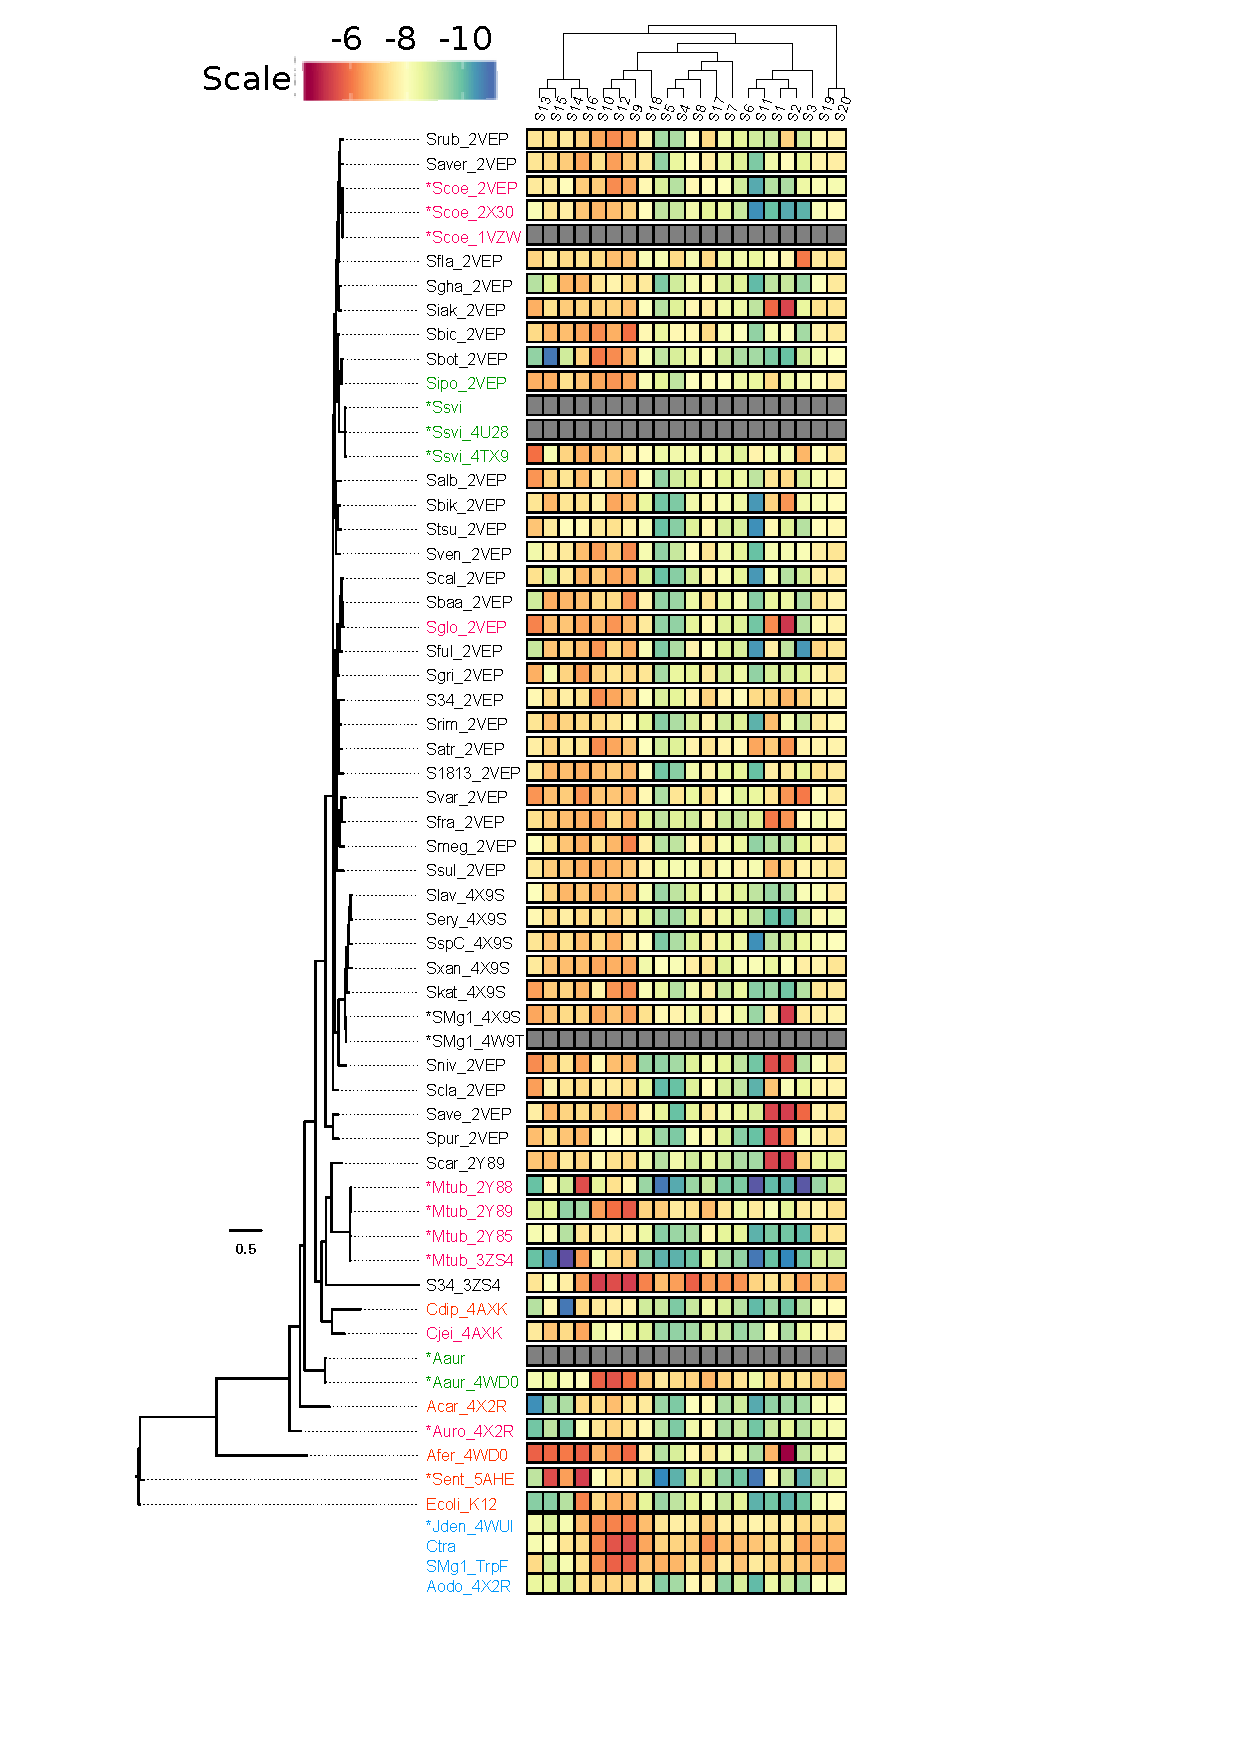
\includegraphics[angle = 0,scale = 1]{chapter2/Figura1_4.pdf}
   \caption[Heatplot docking PriA enzyme Family vs substrates]{\normalsize{Heatplot docking PriA enzyme Family vs substrates}}
   \label{fig:Heatplod PriA docking}
   \end{figure}
  
  PriA S3
  
  \[ 
  \begin{table}
  \begin{tabular}{ l c r l l l l l}
  \hline \\ [-1.5ex]
  organism  &Family & $K_M    $     & $k_{cat}$        & $\frac{k_{cat}}{K_M}$ &Pre MD & Pos MD & Reference  \\ [1ex]
  \hline \\ [-1.5ex]
  Afer        &HisA   & $1.1\pm0.2$   &$  0.05\pm0.001    $& 0.045                  &-10.1    &-12.3       &Noda-García L et al 2015\\ [1ex]
  Ecoli       &HisA   &$  1.6         $&$         4.9       $&3.1                   &-9.9   &-16       &Henn-Sax et al. (2002)\\ [1ex]
  Sent        &HisA   &$  17.0 \pm0.1 $&$ 7.8 \pm 2.4   $&$4.5 × 10^5          $&-10.3  &-20.1     &Söderholm A et al (2015)\\ [1ex]
  Aaur        &PriB   &$  2.1 \pm 0.5 $& $    1.8 \pm 0.2     $&0.9                   &-7.4   &              &verduzco-castro 2016\\ [1ex]
  Sipo        &PriB   &$  3.8\pm0.2     $&$0.82\pm0.02        $&0.21                  &-8.2     &-14.7       &verduzco-castro 2016\\ [1ex]
  SspC        &PriB   &$  11.4\pm3.4  $&$2.53\pm0.74      $&0.22                  &   -8.5    &-12.7     &verduzco-castro 2016\\ [1ex]
  SMg1        &PriB   &$  13.2\pm3.4  $&$0.92\pm0.19      $&0.069                 &-8     &-15.2     &verduzco-castro 2016\\ [1ex]
  Ssvi        &PriB   &$  3.9\pm0.89  $&$0.69\pm0.04      $&0.18                  &-8.2     &-16.7     &verduzco-castro 2016\\ [1ex]
  Scoe        &PriA   &$  3.6\pm0.7     $&$ 1.3\pm0.2     $  &0.4                   &-8.4   &-15       &Noda-García et al (2010)\\ [1ex]
  Sglob       &PriA   & $4.2\pm0.8     $ & $0.74\pm0.03    $   &0.18                  &-9.2     &-16.7       &verduzco-castro\\ [1ex]
  Mtub 2Y85   &priA   &$  19  0.23      $&$0.012  -9.7          $&                      &       &          &Due et al 2011\\ [1ex]
  Mtub 3ZS4   &priA   &$  ?                 $&$-9.9               $&                      &       &          &Due et al 2011 (To be published)\\ [1ex]
  Auro        &priA   &$  4.0 \pm 0.9 $&$0.2 \pm 0.03   $&0.04                    &-9.2       &          &Vazquez-Juarez (2016)\\ [1ex]
  Cjei        &PriA   &$  2.3 \pm 0.2 $&$0.9 \pm 0.08   $&0.39                    &-8.5       &          &Noda-García et al (2013)\\ [1ex]
  Cdip        &subHisA&$  4.4 \pm 0.5 $&$2.6 \pm 0.3      $&0.59                  &-9.2       &          &Noda-García et al (2013)\\ [1ex]
  SMg1 TrpF   &TrpF3  &   -                &-                &-                       &-6.9     &-9.6      &verduzco-castro 2016\\ [1ex]
  Jden        &TrpF3  &   -                &-                &-          -7.2         &-9.4     &$16.8\pm3.3$&    Verduzco-Castro E et al  2016\\ [1ex]
  Acar      &SubHisA& 0.02                     &                 &                        &       &          &            \\ [1ex]
  Aodo        &SubTrpF&       -              &-                  &-                     &       &          &\\ [1ex]
  \hline
  \end{tabular}
  \label{table:name}
  \end{table}
  \]
  
  PriA S7\\
  \$\$ \centering 
  
  \begin{tabular}{ l c r l l l l l}
  \hline \\ [-1.5ex]
  organism  &Family  &  $K_M$ & $k_{cat}$& $\frac{k{cat}}{K_M}$ &Pre MD &Pos MD &Reference  \\ [1ex]
  \hline \\ [-1.5ex]
  Afer      &HisA    &-            &-                &-          &-9.2    &-9        &Noda-García L et al. (2015)   \\ [1ex]
  Ecoli     &HisA    &-            &-                &-          &-9      &-11.1     &Henn-Sax et al. (2002)\\ [1ex]
  Sent      &HisA    &-            & -               &-          &-9.6    &-10.2     &Söderholm A et al (2015)\\ [1ex]
  Aaur      &PriB    &$26.3\pm6.3$ & $0.37\pm 0.09$  & 0.014     &-7.1    &-         &verduzco-castro 2016\\ [1ex]
  Sipo      &PriB    &$60.8\pm1.1$ &$8.25\pm0.4 $    &0.14       &-8      &-8.5      &verduzco-castro 2016 \\ [1ex]
  SspC      &PriB    &$149.9\pm29$ &$1.4\pm0.12 $    &0.009      &-8.5    &-10.8     &verduzco-castro 2016\\ [1ex]
  SMg1      &PriB    &$129.6\pm34$ &$0.29\pm0.04$    &0.0022     &-7.5    &-11       &verduzco-castro 2016\\ [1ex]
  Ssvi      &PriB    &$24.5\pm4.0$ &$1.6\pm0.29 $    &0.067      &-8      &-9.7      &verduzco-castro 2016 \\ [1ex]
  Scoe      &PriA    &$5.0\pm0.08$ &$3.4\pm0.09  $   &0.7        &-8      &-9.4      &Noda-García et al (2010)   \\ [1ex]
  Sglob     &PriA    &$11\pm1.0$  &$3.8\pm0.2  $     &0.34       &-8.7    &-9.4      &verduzco-castro 2016  \\ [1ex]
  Mtub2Y85  &priA    &21         &3.6         &0.17       &-8.6    &          &Due et al 2011                        \\ [1ex] 
  Mtub3ZS4  &priA    &           &            &           &-9.3    &          &Due et al 2011 (To be published)      \\ [1ex] 
  Auro      &priA    &$23 \pm 6.5 $  &$0.5\pm0.05 $&0.02       &-9.3    &          &Vazquez-Juarez (2016)                 \\ [1ex] 
  Cjei      &PriA    &$5.1 \pm1.0$  &$1.6 \pm 0.16 $&0.31       &-9      &          &Noda-García et al (2013)              \\ [1ex]
  Cdip      &subHisA &-          &-           &-          &-8.8    &          &Noda-García et al (2013)              \\ [1ex]
  SMg1 TrpF &TrpF3   &$8.4\pm1.7$    &$10.5\pm2.4$    &1.25       &-7.6    &-9        &verduzco-castro     \\ [1ex] 
  Jden      &TrpF3   &$16.8\pm3.3$   &$27\pm1.6$      &1.6        &-7.6    &-7.7      &verduzco-castro     \\ [1ex] 
  Acar      &SubHisA &Na         &Na          &0.02       &Na      &Na        &Na                                    \\ [1ex] 
  Aodo      &SubTrpF &-          &-           &-          &-       &Na        &Na                                    \\ [1ex]
  
  \hline
  \end{tabular}
  
  \label{table:mi table}\$\$
  
  Con actividad de FolE i.e activa para el compuesto V Adams et al (2014)
  Genome size vs Total antismash cluster coloured by order
  
  \begin{figure}[h!tbp]
  \centering
  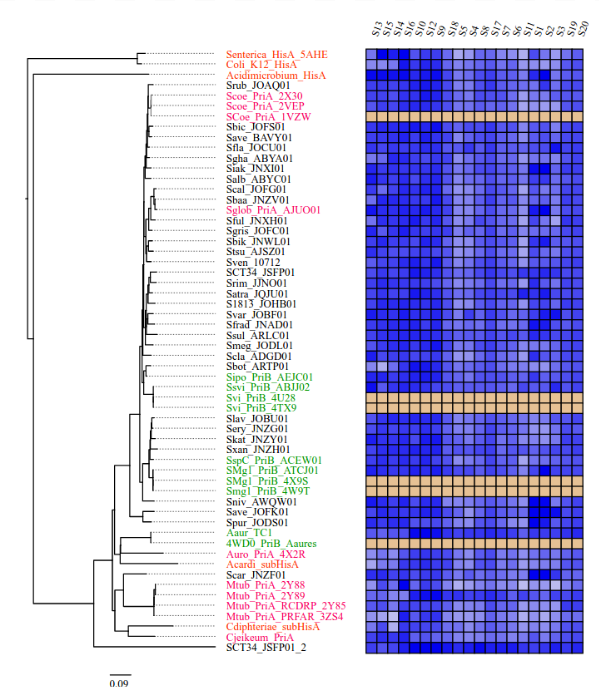
\includegraphics[angle = 0,scale = 0.6]{chapter2/PriAHeatPot.png}
  \caption[Heat Plot PriA Streptomyces vs other subtrates]{\normalsize{Heat Plot PriA Streptomyces vs other subtrates}}
  \label{fig:PriADocking}
  \end{figure}
  
  Docker simulation were calculated for Streptomyces enzymes\\
  Genome size vs Total antismash cluster coloured by order
  
  \begin{figure}[h!tbp]
  \centering
  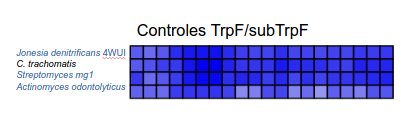
\includegraphics[angle = 0,scale = 0.6]{chapter2/TrpFHeatPlot.png}
  \caption[Heat Plot TrpF Streptomyces vs other subtrates]{\normalsize{Heat Plot TrpF Streptomyces vs other subtrates}}
  \label{fig:TrpFDocking}
  \end{figure}
  
  \section{Latex no Docking}\label{latex-no-docking}
  
  We can further look into the properties of the largest value here for
  American Airlines Inc. To do so, we can isolate the row corresponding to
  the arrival delay of 1539 minutes for American in our original
  \texttt{flights} dataset.
  
  \begin{Shaded}
  \begin{Highlighting}[]
  \CommentTok{#flights %>% dplyr::filter(arr_delay == 1539, carrier_name == "American Airlines Inc.") %>%}
    \CommentTok{#dplyr::select(-c(month, day, carrier, dest_name, hour, minute, carrier_name, arr_delay))}
  \end{Highlighting}
  \end{Shaded}
  
  We see that the flight occurred on March 3rd and departed a little after
  2 PM on its way to Dallas/Fort Worth. Lastly, we show how we can
  visualize the arrival delay of all departing flights from Portland on
  March 3rd against time of departure.
  
  \begin{Shaded}
  \begin{Highlighting}[]
  \CommentTok{#flights %>% dplyr::filter(month == 3, day == 3) %>%}
  \CommentTok{#  ggplot(aes(x = dep_time, y = arr_delay)) +geom_point()}
  \end{Highlighting}
  \end{Shaded}
  
  \TeX~is the best way to typeset mathematics. Donald Knuth designed
  \TeX~when he got frustrated at how long it was taking the typesetters to
  finish his book, which contained a lot of mathematics. One nice feature
  of \emph{R Markdown} is its ability to read \LaTeX~code directly.
  
  If you are doing a thesis that will involve lots of math, you will want
  to read the following section which has been commented out. If you're
  not going to use math, skip over or delete this next commented section.
  
  \section{Chemistry 101: Symbols}\label{chemistry-101-symbols}
  
  Chemical formulas will look best if they are not italicized. Get around
  math mode's automatic italicizing in \LaTeX~by using the argument
  \texttt{\$\textbackslash{}mathrm\{formula\ here\}\$}, with your formula
  inside the curly brackets. (Notice the use of the backticks here which
  enclose text that acts as code.)
  
  So, \(\mathrm{Fe_2^{2+}Cr_2O_4}\) is written
  \texttt{\$\textbackslash{}mathrm\{Fe\_2\^{}\{2+\}Cr\_2O\_4\}\$}.
  
  \noindent Exponent or Superscript: \(\mathrm{O^-}\)
  
  \noindent Subscript: \(\mathrm{CH_4}\)
  
  To stack numbers or letters as in \(\mathrm{Fe_2^{2+}}\), the subscript
  is defined first, and then the superscript is defined.
  
  \noindent Angstrom: \({\AA}\)
  
  \noindent Bullet: CuCl \(\bullet\) \(\mathrm{7H_{2}O}\)
  
  \noindent Double Dagger: \(\ddag\)
  
  \noindent Delta: \(\Delta\)
  
  \noindent Reaction Arrows: \(\longrightarrow\) or
  \(\xrightarrow{solution}\)
  
  \noindent Resonance Arrows: \(\leftrightarrow\)
  
  \noindent Reversible Reaction Arrows: \(\rightleftharpoons\) or
  \(\xrightleftharpoons[ ]{solution}\) (the latter requires the
  \texttt{chemarr} \LaTeX~package which is automatically loaded in this
  template)
  
  \subsection{Typesetting reactions}\label{typesetting-reactions}
  
  You may wish to put your reaction in a figure environment, which means
  that \LaTeX~will place the reaction where it fits and you can have a
  figure caption. You'll see further description of this \textbf{R}
  \texttt{label} function in \protect\hyperlink{refux5flabels}{}. (Note
  the use of the double backslash here as well as the
  \texttt{echo\ =\ FALSE} which hides the code from the output.)
  
  \begin{figure}[h!tbp]
  \begin{center}
  $\mathrm{C_6H_{12}O_6  + 6O_2} \longrightarrow \mathrm{6CO_2 + 6H_2O}$
  \caption{Combustion of glucose}
  \label{fig:comb-gluc}
  \end{center}
  \end{figure}
  
  \subsection{Other examples of
  reactions}\label{other-examples-of-reactions}
  
  \(\mathrm{NH_4Cl_{(s)}}\) \(\rightleftharpoons\)
  \(\mathrm{NH_{3(g)}+HCl_{(g)}}\)
  
  \noindent \(\mathrm{MeCH_2Br + Mg}\) \(\xrightarrow[below]{above}\)
  \(\mathrm{MeCH_2\bullet Mg \bullet Br}\)
  
  \section{Physics}\label{physics}
  
  Many of the symbols you will need can be found on the math page
  \url{http://web.reed.edu/cis/help/latex/math.html} and the Comprehensive
  \LaTeX~Symbol Guide
  (\url{http://mirror.utexas.edu/ctan/info/symbols/comprehensive/symbols-letter.pdf}).
  
  \section{Biology}\label{biology}
  
  You will probably find the resources at
  \url{http://www.lecb.ncifcrf.gov/~toms/latex.html} helpful, particularly
  the links to bsts for various journals. You may also be interested in
  TeXShade for nucleotide typesetting
  (\url{http://homepages.uni-tuebingen.de/beitz/txe.html}). Be sure to
  read the proceeding chapter on graphics and tables.
  
  \begin{Shaded}
  \begin{Highlighting}[]
  \KeywordTok{sessionInfo}\NormalTok{()}
  \end{Highlighting}
  \end{Shaded}
  
  \begin{verbatim}
  R version 3.3.2 (2016-10-31)
  Platform: x86_64-pc-linux-gnu (64-bit)
  Running under: Ubuntu 14.04.5 LTS
  
  locale:
   [1] LC_CTYPE=en_US.UTF-8          LC_NUMERIC=C                 
   [3] LC_TIME=es_MX.UTF-8           LC_COLLATE=en_US.UTF-8       
   [5] LC_MONETARY=es_MX.UTF-8       LC_MESSAGES=en_US.UTF-8      
   [7] LC_PAPER=es_MX.UTF-8          LC_NAME=es_MX.UTF-8          
   [9] LC_ADDRESS=es_MX.UTF-8        LC_TELEPHONE=es_MX.UTF-8     
  [11] LC_MEASUREMENT=es_MX.UTF-8    LC_IDENTIFICATION=es_MX.UTF-8
  
  attached base packages:
  [1] parallel  stats     graphics  grDevices utils     datasets  methods  
  [8] base     
  
  other attached packages:
   [1] xlsx_0.5.7          xlsxjars_0.6.1      rJava_0.9-8        
   [4] scales_0.4.1        Biobase_2.34.0      BiocGenerics_0.20.0
   [7] genstats_0.1.02     RColorBrewer_1.1-2  reshape_0.8.6      
  [10] plyr_1.8.4          ape_4.0             knitr_1.15.1       
  [13] ggplot2_2.2.1       dplyr_0.5.0         reedtemplates_0.1  
  [16] devtools_1.12.0    
  
  loaded via a namespace (and not attached):
   [1] Rcpp_0.12.9      highr_0.6        tools_3.3.2      digest_0.6.12   
   [5] evaluate_0.10    memoise_1.0.0    tibble_1.2       gtable_0.2.0    
   [9] nlme_3.1-131     lattice_0.20-34  DBI_0.5-1        yaml_2.1.14     
  [13] withr_1.0.2      stringr_1.1.0    rprojroot_1.2    grid_3.3.2      
  [17] R6_2.2.0         rmarkdown_1.3    magrittr_1.5     backports_1.0.5 
  [21] htmltools_0.3.5  assertthat_0.1   colorspace_1.3-2 labeling_0.3    
  [25] stringi_1.1.2    lazyeval_0.2.0   munsell_0.4.3   
  \end{verbatim}
  
  \hypertarget{refux5flabels}{\chapter{Archaea EvoMining
  Results}\label{refux5flabels}}
  
  During the decade between 1970 and 1980, Archaea was recognized as new
  life domain, a kingdom different from Bacteria and Eucarya in an
  exciting first great application of 16S
  phylogeny{[}\protect\hyperlink{ref-woeseux5fphylogeneticux5f1977}{115}{]}
  . Main differences between this kingdoms are that Archaeal DNA is not
  arranged in a nucleus as in Eucarya and Archaeal celular walls are not
  composed from peptidoglycans as in Bacteria. Archaeal proteins may be
  higlhy valuable to biotechnology industry for their great stability due
  to extreme temperature, PH and salt content conditions on Archeal
  habitats. Despite no Archaeal Natural products biosynthetic gene
  clusters (BGC's) has been reported on MiBIG, Archaea do have BGC's, some
  of them seems to be acquired by horizontal gene transfer (HGT) like
  methano nrps \{search reference\}. Other Archeal natural products known
  are archaeosins, Diketopiperazines, Acyl Homoserine Lactones,
  Exopolysaccharides, Carotenoids, Biosurfactants, Phenazines and Organic
  Solutes but this knowledge is not comparable to Bacterial BGC's
  knowledge{[}\protect\hyperlink{ref-charlesworthux5funtappedux5f2015}{99}{]}.
  
  Natural products biosynthetic gene clusters search is actually performed
  using either \emph{high-confidence/low-novelty or
  low-confidence/high-novelty} bioinformatic approaches
  {[}\protect\hyperlink{ref-medemaux5fcomputationalux5f2015}{50}{]}. High
  confidence methods compares query sequences with previously known BGC's
  such as nrps or PKS, examples of this algorithms are antiSMASH and
  clusterfinder {[}\textbf{???}?{]}. EvoMining searches on expansions from
  central metabolic pathways enzyme families, it has been classified as
  low confidence/high novelty method. EvoMining has proved useful on
  Actinobacteria phylum where its use lead to Arseno-compounds discovery
  {[}\protect\hyperlink{ref-cruz-moralesux5fphylogenomicux5f2016}{65}{]}.
  Also on Actinobacteria antiSMASH analysis on 1245 genomes found 774
  different classes of natural products, the same analysis on 876 Archaeal
  genomes, a full kingdom, identifies only 35 BGC's classes. So either
  Archaea does not have natural products BGC's or this are not yet known.
  Next paragraph deals with a possible approach about how natural products
  BGC's can be find.
  
  Archaea resembled Bacteria in that Archaea uses horizontal gene transfer
  as a genic interchange mecanism, Archaeal genomes contains operons
  {[}\protect\hyperlink{ref-howlandux5fsurprisingux5f2000}{118}{]} and in
  general there is introns absence\{Reference to Computational Methods for
  Understanding Bacterial and Archaeal Genomes\}. Archaeas do have
  introns, but they are mainly located on genes that encodes ribosomal and
  transfer RNA
  {[}\protect\hyperlink{ref-howlandux5fsurprisingux5f2000}{118}{]}.
  General lack of introns allows automatic genome annotation, operons gene
  organization permits functional inference to a certain degree and HGT
  contribute to expansions on Archaeal genomes. Some phylum on Archaea has
  an open pangenome, and as we will show on this chapter some Archaea has
  central pathway expansions. Enzyme families from central pathways
  expansions, open pangenome and operon organization made EvoMining
  succesful on Actinobacteria, this lead us to think that evoMining is
  suitable to analize Archaeal genomes, even more since EvoMining is a
  method oriented to use evolution and its not entirelyy based on previous
  knowledge of BGC's sequences if evolutionary logic behave on Archaea as
  on bacteria, new BGC's classes may be be found on Archaea.
  
  EvoMining is a trade off between conserved known central metabolic
  function and enough expansions divergence on sequence and on clusters to
  divergence
  
  \section{Tables}\label{tables}
  
  \begin{longtable}[c]{@{}cc@{}}
  \caption{Families on Archaeabacteria \label{tab:inher}}\tabularnewline
  \toprule
  Factors & Correlation between Parents \& Child\tabularnewline
  \midrule
  \endfirsthead
  \toprule
  Factors & Correlation between Parents \& Child\tabularnewline
  \midrule
  \endhead
  GenomeDB & 876\tabularnewline
  Phylum & 12\tabularnewline
  Order & 23\tabularnewline
  \bottomrule
  \end{longtable}
  
  \clearpage
  
  First lets investigate if Archaea has expansions on families within
  central metabolic routes. Since main metabolic pathways are shared
  between Bacteria and Archaea makes sense to assemble Archeal EvoMining
  central database by using orthologous from Actinobacteria evoMining
  central pathways.
  
  \subsection{Expansions BoxPlot by metabolic
  family}\label{expansions-boxplot-by-metabolic-family}
  
  \begin{Shaded}
  \begin{Highlighting}[]
  \KeywordTok{label}\NormalTok{(}\DataTypeTok{path =} \StringTok{"chapter3/expansion_plotArchaeas.pdf"}\NormalTok{, }\DataTypeTok{caption =} \StringTok{"Expansions Boxplot"}\NormalTok{,}\DataTypeTok{label =} \StringTok{"Archaea_expansion_boxplot"}\NormalTok{, }\DataTypeTok{type =} \StringTok{"figure"}\NormalTok{,}\DataTypeTok{scale=}\StringTok{".7"}\NormalTok{)}
  \end{Highlighting}
  \end{Shaded}
  
  \begin{figure}[h!tbp]
  \centering
  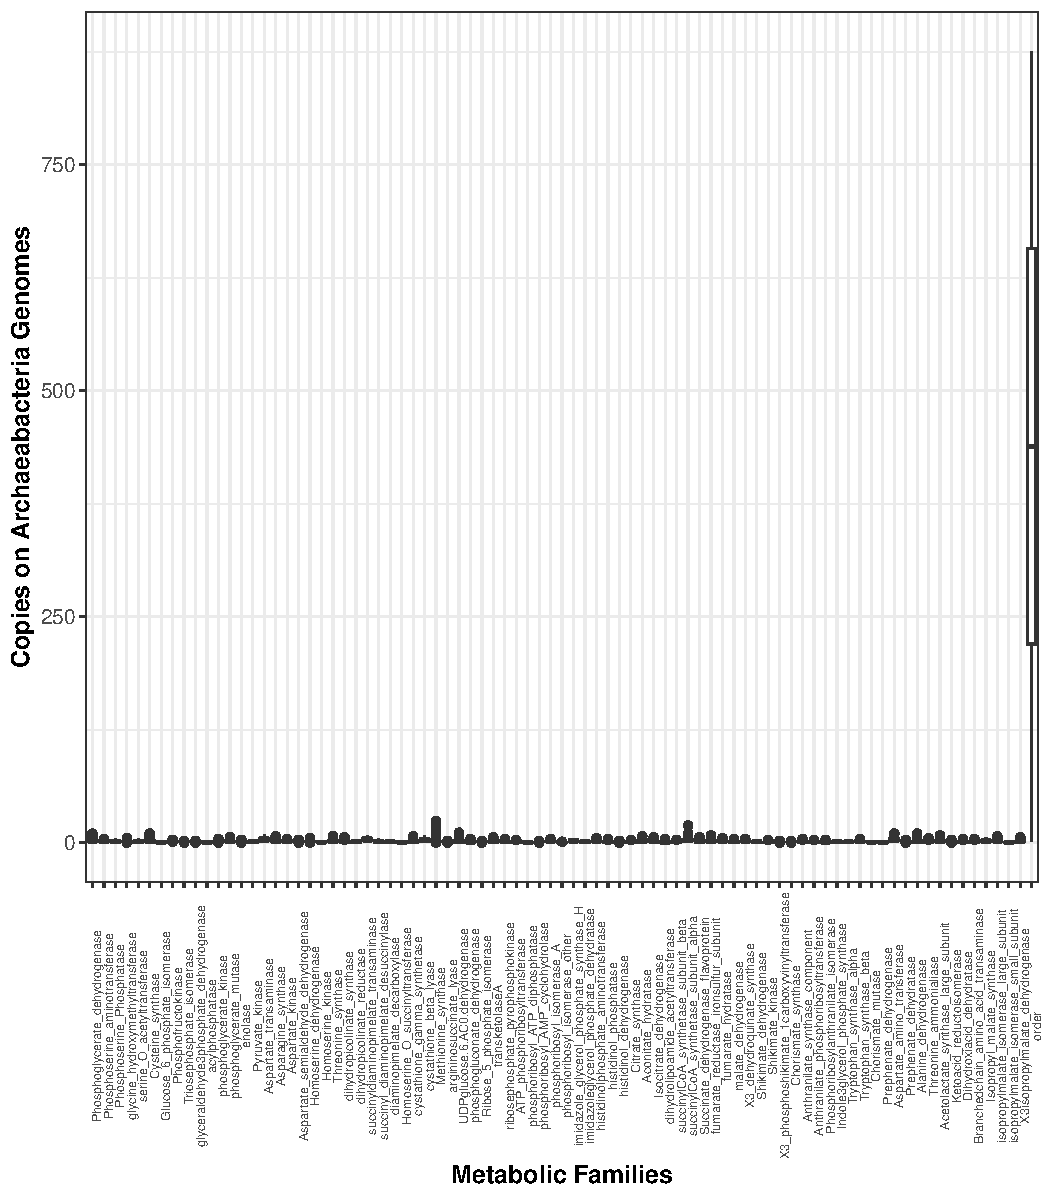
\includegraphics[angle = 0,scale = .7]{chapter3/expansion_plotArchaeas.pdf}
  \caption[Expansions Boxplot]{\normalsize{Expansions Boxplot}}
  \label{fig:Archaea_expansion_boxplot}
  \end{figure}
  
  Here is a reference to the expansion boxplot:
  \autoref{fig:Archaea_expansion_boxplot}.\\
  \clearpage 
  
  \subsection{Expansions BoxPlot by metabolic family by
  phylum}\label{expansions-boxplot-by-metabolic-family-by-phylum}
  
  \begin{Shaded}
  \begin{Highlighting}[]
  \CommentTok{#+ geom_jitter()}
  \CommentTok{#aes(fill = factor(vs))}
  
  \NormalTok{ArchaeasTotalBP.m<-}\KeywordTok{merge}\NormalTok{(ArchaeasHeatPlot,ArchaeasTaxa,}\DataTypeTok{by.x=}\StringTok{"RastId"}\NormalTok{,}\DataTypeTok{by.y=}\StringTok{"RastId"}\NormalTok{) ## works as expected}
  \NormalTok{ArchaeasHeatPlotBP.m <-}\StringTok{ }\KeywordTok{melt}\NormalTok{(ArchaeasTotalBP.m,}\DataTypeTok{id =}\KeywordTok{c}\NormalTok{(}\StringTok{"RastId"}\NormalTok{,}\StringTok{"Name"}\NormalTok{,}\StringTok{"SuperPhylum"}\NormalTok{,}\StringTok{"Phylum"}\NormalTok{,}\StringTok{"Class"}\NormalTok{,}\StringTok{"Order"}\NormalTok{,}\StringTok{"Family"}\NormalTok{,}\StringTok{"RastNo"}\NormalTok{,}\StringTok{"Size"}\NormalTok{,}\StringTok{"Contigs"}\NormalTok{))}
  \NormalTok{ArchaeasHeatPlotBP.m<-}\KeywordTok{subset}\NormalTok{(ArchaeasHeatPlotBP.m,variable!=}\StringTok{"TOTAL"}\NormalTok{) ## works as expected}
  \NormalTok{ArchaeasHeatPlotBP.m<-}\KeywordTok{subset}\NormalTok{(ArchaeasHeatPlotBP.m,variable!=}\StringTok{"TOTAL"}\NormalTok{) ## works as expected}
  
  \NormalTok{## Each metabolic pathway se parte por phylum coloreado por order}
  
  \CommentTok{#3PGA_AMINOACIDS}
  \CommentTok{#Glycolysis}
  \CommentTok{#OXALACETATE_AMINOACIDS}
  \CommentTok{#R5P_AMINOACIDS}
  \CommentTok{#TCA}
  \CommentTok{#E4P_AMINO_ACIDS}
  \CommentTok{#PYR_THR_AA}
  
  \NormalTok{## Genome size}
  \KeywordTok{ggplot}\NormalTok{(ArchaeasHeatPlotBP.m, }\KeywordTok{aes}\NormalTok{(}\DataTypeTok{x=}\NormalTok{ArchaeasHeatPlotBP.m$Phylum, }\DataTypeTok{y=}\NormalTok{ArchaeasHeatPlotBP.m$Size))+}\StringTok{ }\KeywordTok{geom_boxplot}\NormalTok{() +}\KeywordTok{theme}\NormalTok{(}\DataTypeTok{plot.title =} \KeywordTok{element_text}\NormalTok{(}\DataTypeTok{size =} \DecValTok{14}\NormalTok{, }\DataTypeTok{face =} \StringTok{"bold"}\NormalTok{), }\DataTypeTok{text =} \KeywordTok{element_text}\NormalTok{(}\DataTypeTok{size =} \DecValTok{12}\NormalTok{), }\DataTypeTok{axis.title =} \KeywordTok{element_text}\NormalTok{(}\DataTypeTok{face=}\StringTok{"bold"}\NormalTok{), }\DataTypeTok{axis.text.x=}\KeywordTok{element_text}\NormalTok{(}\DataTypeTok{angle =} \DecValTok{90}\NormalTok{,}\DataTypeTok{size =} \DecValTok{6}\NormalTok{), }\DataTypeTok{legend.position =} \StringTok{"bottom"}\NormalTok{)+}\StringTok{ }\KeywordTok{labs}\NormalTok{(}\DataTypeTok{x =} \StringTok{"Copies on Archaeabacteria taxonomic groups"}\NormalTok{, }\DataTypeTok{y =} \StringTok{"Genome size"}\NormalTok{,}\DataTypeTok{text =} \KeywordTok{element_text}\NormalTok{(}\DataTypeTok{size=}\DecValTok{12}\NormalTok{))+}\KeywordTok{theme_bw}\NormalTok{()}
  \end{Highlighting}
  \end{Shaded}
  
  \begin{center}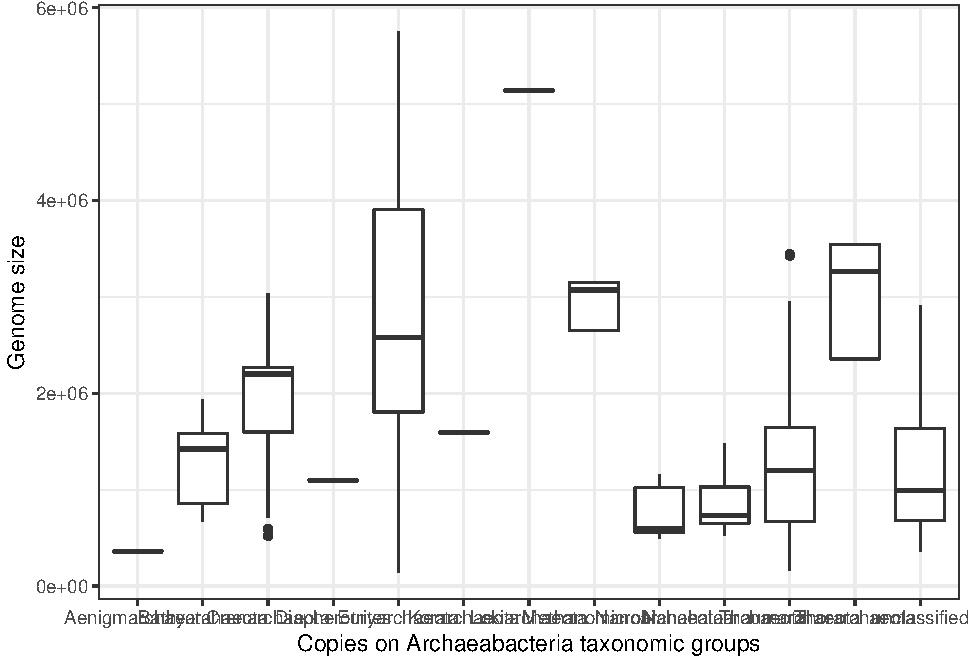
\includegraphics{tesis_files/figure-latex/ArcheaeBoxPlotByPhylum-1} \end{center}
  
  \begin{Shaded}
  \begin{Highlighting}[]
  \CommentTok{#+ geom_jitter(aes(color=ArchaeasHeatPlotBP.m$Phylum))}
  
  
  \NormalTok{## Halobacteria}
  \NormalTok{MetFam_BP.m=}\KeywordTok{subset}\NormalTok{(ArchaeasHeatPlotBP.m,Phylum==}\StringTok{"Euryarchaeota"}\NormalTok{)}
  \KeywordTok{ggplot}\NormalTok{(MetFam_BP.m, }\KeywordTok{aes}\NormalTok{(}\DataTypeTok{x=}\NormalTok{MetFam_BP.m$Order, }\DataTypeTok{y=}\NormalTok{MetFam_BP.m$Size))+}\StringTok{ }\KeywordTok{geom_boxplot}\NormalTok{() +}\KeywordTok{theme}\NormalTok{(}\DataTypeTok{plot.title =} \KeywordTok{element_text}\NormalTok{(}\DataTypeTok{size =} \DecValTok{14}\NormalTok{, }\DataTypeTok{face =} \StringTok{"bold"}\NormalTok{), }\DataTypeTok{text =} \KeywordTok{element_text}\NormalTok{(}\DataTypeTok{size =} \DecValTok{12}\NormalTok{), }\DataTypeTok{axis.title =} \KeywordTok{element_text}\NormalTok{(}\DataTypeTok{face=}\StringTok{"bold"}\NormalTok{), }\DataTypeTok{axis.text.x=}\KeywordTok{element_text}\NormalTok{(}\DataTypeTok{angle =} \DecValTok{90}\NormalTok{,}\DataTypeTok{size =} \DecValTok{10}\NormalTok{), }\DataTypeTok{legend.position =} \StringTok{"bottom"}\NormalTok{)+}\StringTok{ }\KeywordTok{labs}\NormalTok{(}\DataTypeTok{x =} \StringTok{"Halobacteria orders size taxonomic groups"}\NormalTok{, }\DataTypeTok{y =} \StringTok{"Genome size"}\NormalTok{,}\DataTypeTok{text =} \KeywordTok{element_text}\NormalTok{(}\DataTypeTok{size=}\DecValTok{12}\NormalTok{)) +}\StringTok{ }\KeywordTok{geom_jitter}\NormalTok{(}\KeywordTok{aes}\NormalTok{(}\DataTypeTok{color=}\NormalTok{Family))}
  \end{Highlighting}
  \end{Shaded}
  
  \begin{center}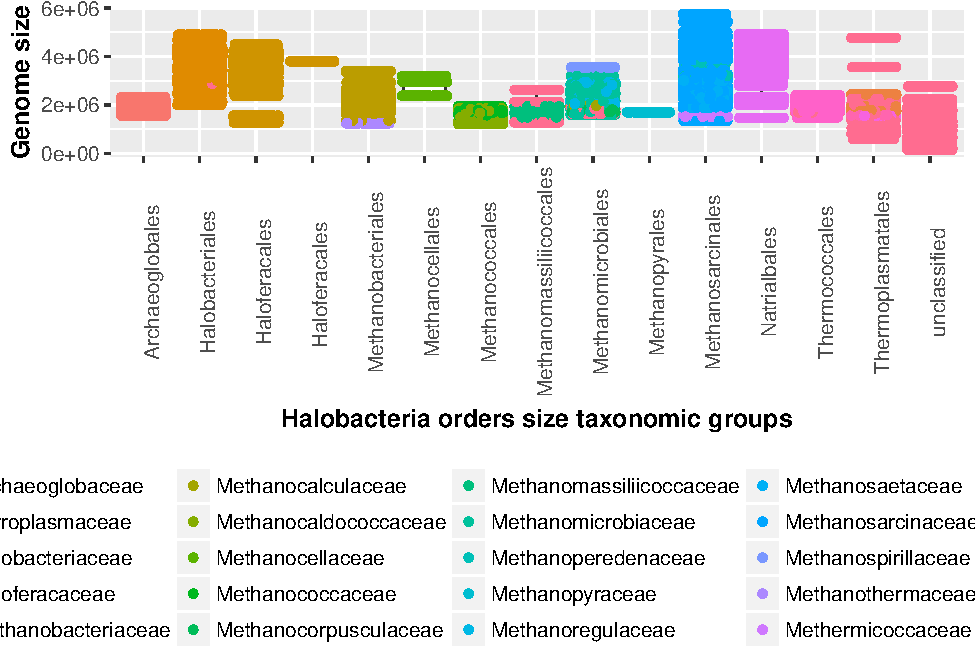
\includegraphics{tesis_files/figure-latex/ArcheaeBoxPlotByPhylum-2} \end{center}
  
  \begin{Shaded}
  \begin{Highlighting}[]
  \CommentTok{#MetFam_BP.m=subset(ArchaeasHeatPlotBP.m,Family=="Methanosarcinaceae")}
  \CommentTok{#ggplot(MetFam_BP.m, aes(x=MetFam_BP.m$Size, y=MetFam_BP.m$value))}
  \CommentTok{#+theme(plot.title = element_text(size = 14, face = "bold"), text = element_text(size = 12), axis.title = element_text(face="bold"), axis.text.x=element_text(angle = 90,size = 10), legend.position = "bottom")+ labs(x = "Copies on Archaeabacteria taxonomic groups", y = "Genome size",text = element_text(size=12)) }
  
  
    \CommentTok{#geom_jitter(aes(color=ArchaeasHeatPlotBP.m$Phylum))# + facet_grid(. ~ Phylum)+theme_bw()}
  
  
  \NormalTok{## Metabolic Pathways}
  \NormalTok{MetFam=}\KeywordTok{subset}\NormalTok{(ArchaeasCentral,Pathway==}\StringTok{"PPP"}\NormalTok{)}
  \NormalTok{MetFam_BP.m=ArchaeasHeatPlotBP.m[ArchaeasHeatPlotBP.m$variable %in%}\StringTok{ }\NormalTok{MetFam$Enzyme,]}
  \KeywordTok{ggplot}\NormalTok{(MetFam_BP.m, }\KeywordTok{aes}\NormalTok{(}\DataTypeTok{x=}\NormalTok{MetFam_BP.m$variable, }\DataTypeTok{y=}\NormalTok{MetFam_BP.m$value, }\DataTypeTok{fill=}\NormalTok{Order))+}\StringTok{ }\KeywordTok{labs}\NormalTok{(}\DataTypeTok{x =} \StringTok{"Metabolic PPP Families"}\NormalTok{, }\DataTypeTok{y =} \StringTok{"Copies on Archaeabacteria Genomes"}\NormalTok{,}\DataTypeTok{text =} \KeywordTok{element_text}\NormalTok{(}\DataTypeTok{size=}\DecValTok{12}\NormalTok{)) +}\StringTok{ }\KeywordTok{geom_boxplot}\NormalTok{() +}\StringTok{ }\KeywordTok{facet_grid}\NormalTok{(. ~}\StringTok{ }\NormalTok{Phylum)+}\KeywordTok{theme_bw}\NormalTok{() +}\KeywordTok{theme}\NormalTok{(}\DataTypeTok{plot.title =} \KeywordTok{element_text}\NormalTok{(}\DataTypeTok{size =} \DecValTok{14}\NormalTok{, }\DataTypeTok{face =} \StringTok{"bold"}\NormalTok{), }\DataTypeTok{text =} \KeywordTok{element_text}\NormalTok{(}\DataTypeTok{size =} \DecValTok{12}\NormalTok{), }\DataTypeTok{axis.title =} \KeywordTok{element_text}\NormalTok{(}\DataTypeTok{face=}\StringTok{"bold"}\NormalTok{), }\DataTypeTok{axis.text.x=}\KeywordTok{element_text}\NormalTok{(}\DataTypeTok{angle =} \DecValTok{90}\NormalTok{,}\DataTypeTok{size =} \DecValTok{6}\NormalTok{), }\DataTypeTok{legend.position =} \StringTok{"bottom"}\NormalTok{)}
  \end{Highlighting}
  \end{Shaded}
  
  \begin{center}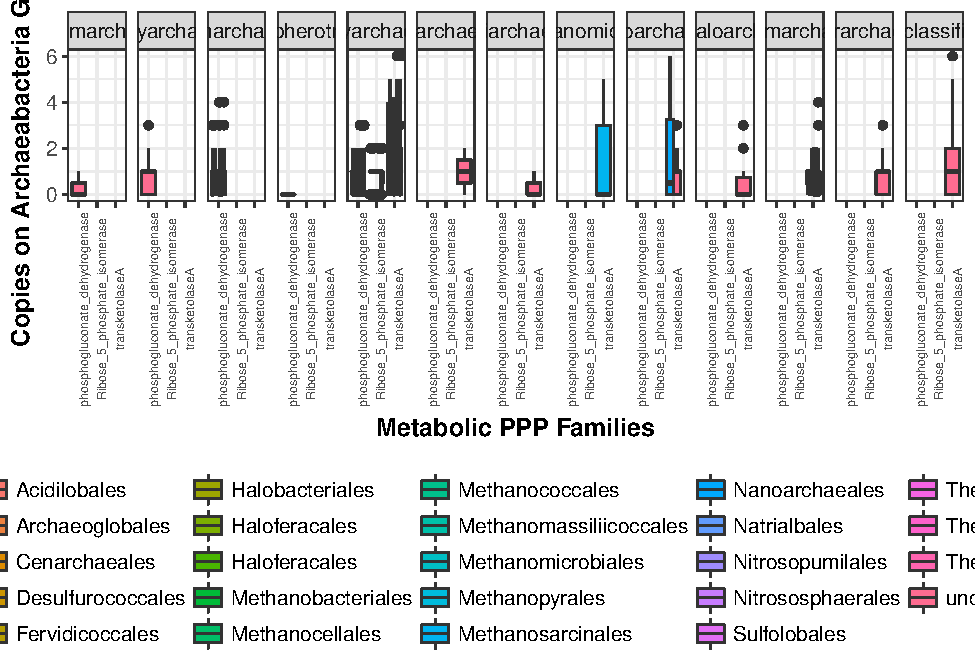
\includegraphics{tesis_files/figure-latex/ArcheaeBoxPlotByPhylum-3} \end{center}
  
  \begin{Shaded}
  \begin{Highlighting}[]
  \CommentTok{#+ geom_jitter(aes(color=MetFam_BP.m$Phylum))       }
  
  \NormalTok{MetFam=}\KeywordTok{subset}\NormalTok{(ArchaeasCentral,Pathway==}\StringTok{"3PGA_AMINOACIDS"}\NormalTok{)}
  \NormalTok{MetFam_BP.m=ArchaeasHeatPlotBP.m[ArchaeasHeatPlotBP.m$variable %in%}\StringTok{ }\NormalTok{MetFam$Enzyme,]}
  \KeywordTok{ggplot}\NormalTok{(MetFam_BP.m, }\KeywordTok{aes}\NormalTok{(}\DataTypeTok{x=}\NormalTok{MetFam_BP.m$variable, }\DataTypeTok{y=}\NormalTok{MetFam_BP.m$value, }\DataTypeTok{fill=}\NormalTok{Order))+}\StringTok{ }\KeywordTok{labs}\NormalTok{(}\DataTypeTok{x =} \StringTok{"Metabolic PGA_AMINOACIDS Families"}\NormalTok{, }\DataTypeTok{y =} \StringTok{"Copies on Archaeabacteria Genomes"}\NormalTok{,}\DataTypeTok{text =} \KeywordTok{element_text}\NormalTok{(}\DataTypeTok{size=}\DecValTok{12}\NormalTok{)) +}\StringTok{ }\KeywordTok{geom_boxplot}\NormalTok{() +}\StringTok{ }\KeywordTok{facet_grid}\NormalTok{(. ~}\StringTok{ }\NormalTok{Phylum)+}\KeywordTok{theme_bw}\NormalTok{()+}\KeywordTok{theme}\NormalTok{(}\DataTypeTok{plot.title =} \KeywordTok{element_text}\NormalTok{(}\DataTypeTok{size =} \DecValTok{14}\NormalTok{, }\DataTypeTok{face =} \StringTok{"bold"}\NormalTok{), }\DataTypeTok{text =} \KeywordTok{element_text}\NormalTok{(}\DataTypeTok{size =} \DecValTok{12}\NormalTok{), }\DataTypeTok{axis.title =} \KeywordTok{element_text}\NormalTok{(}\DataTypeTok{face=}\StringTok{"bold"}\NormalTok{), }\DataTypeTok{axis.text.x=}\KeywordTok{element_text}\NormalTok{(}\DataTypeTok{angle =} \DecValTok{90}\NormalTok{,}\DataTypeTok{size =} \DecValTok{6}\NormalTok{), }\DataTypeTok{legend.position =} \StringTok{"bottom"}\NormalTok{)}
  \end{Highlighting}
  \end{Shaded}
  
  \begin{center}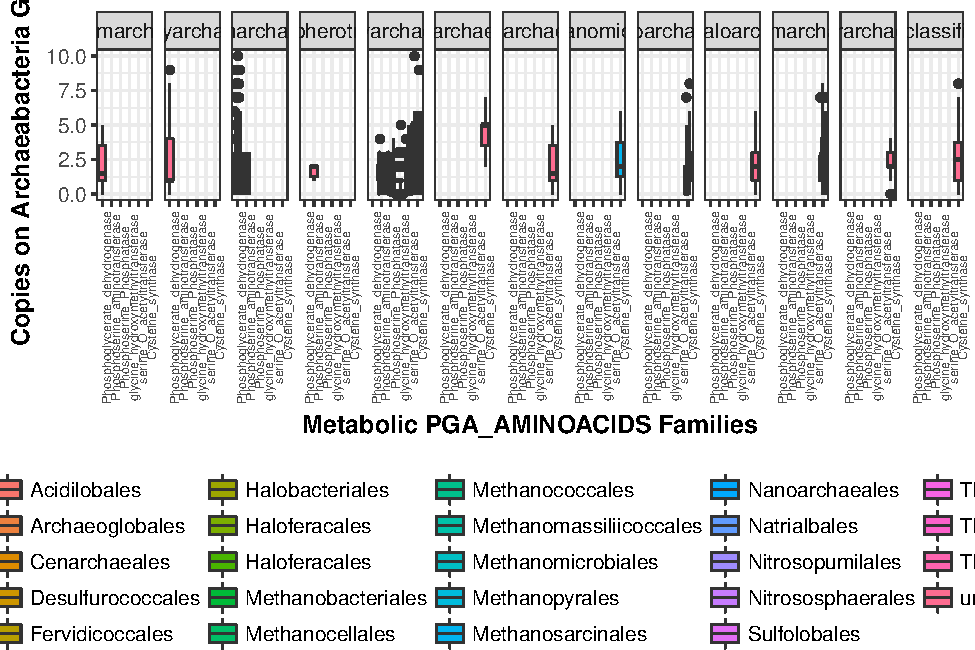
\includegraphics{tesis_files/figure-latex/ArcheaeBoxPlotByPhylum-4} \end{center}
  
  \begin{Shaded}
  \begin{Highlighting}[]
  \CommentTok{#+ geom_jitter(aes(color=MetFam_BP.m$Phylum))}
  
  \NormalTok{MetFam=}\KeywordTok{subset}\NormalTok{(ArchaeasCentral,Pathway==}\StringTok{"Glycolysis"}\NormalTok{)}
  \NormalTok{MetFam_BP.m=ArchaeasHeatPlotBP.m[ArchaeasHeatPlotBP.m$variable %in%}\StringTok{ }\NormalTok{MetFam$Enzyme,]}
  \KeywordTok{ggplot}\NormalTok{(MetFam_BP.m, }\KeywordTok{aes}\NormalTok{(}\DataTypeTok{x=}\NormalTok{MetFam_BP.m$variable, }\DataTypeTok{y=}\NormalTok{MetFam_BP.m$value, }\DataTypeTok{fill=}\NormalTok{Order))+}\StringTok{ }\KeywordTok{labs}\NormalTok{(}\DataTypeTok{x =} \StringTok{"Metabolic Glycolysis Families"}\NormalTok{, }\DataTypeTok{y =} \StringTok{"Copies on Archaeabacteria Genomes"}\NormalTok{,}\DataTypeTok{text =} \KeywordTok{element_text}\NormalTok{(}\DataTypeTok{size=}\DecValTok{12}\NormalTok{)) +}\StringTok{ }\KeywordTok{geom_boxplot}\NormalTok{() +}\StringTok{ }\KeywordTok{facet_grid}\NormalTok{(. ~}\StringTok{ }\NormalTok{Phylum)+}\KeywordTok{theme_bw}\NormalTok{()+}\KeywordTok{theme}\NormalTok{(}\DataTypeTok{plot.title =} \KeywordTok{element_text}\NormalTok{(}\DataTypeTok{size =} \DecValTok{14}\NormalTok{, }\DataTypeTok{face =} \StringTok{"bold"}\NormalTok{), }\DataTypeTok{text =} \KeywordTok{element_text}\NormalTok{(}\DataTypeTok{size =} \DecValTok{12}\NormalTok{), }\DataTypeTok{axis.title =} \KeywordTok{element_text}\NormalTok{(}\DataTypeTok{face=}\StringTok{"bold"}\NormalTok{), }\DataTypeTok{axis.text.x=}\KeywordTok{element_text}\NormalTok{(}\DataTypeTok{angle =} \DecValTok{90}\NormalTok{,}\DataTypeTok{size =} \DecValTok{6}\NormalTok{), }\DataTypeTok{legend.position =} \StringTok{"bottom"}\NormalTok{)}
  \end{Highlighting}
  \end{Shaded}
  
  \begin{center}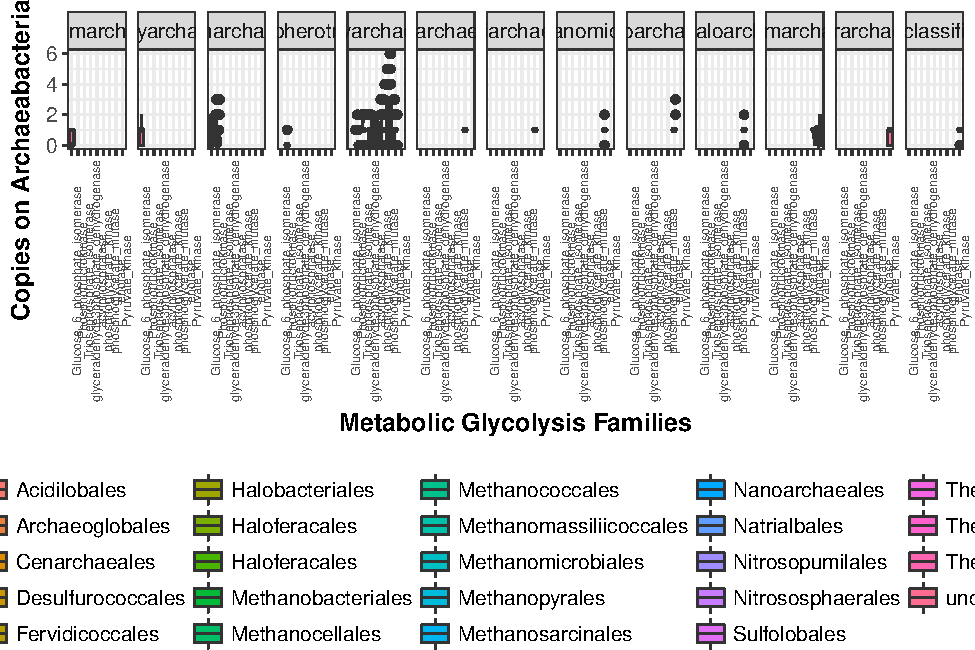
\includegraphics{tesis_files/figure-latex/ArcheaeBoxPlotByPhylum-5} \end{center}
  
  \begin{Shaded}
  \begin{Highlighting}[]
  \CommentTok{#+ geom_jitter(aes(color=MetFam_BP.m$Phylum))}
  
  \NormalTok{MetFam=}\KeywordTok{subset}\NormalTok{(ArchaeasCentral,Pathway==}\StringTok{"OXALACETATE_AMINOACIDS"}\NormalTok{)}
  \NormalTok{MetFam_BP.m=ArchaeasHeatPlotBP.m[ArchaeasHeatPlotBP.m$variable %in%}\StringTok{ }\NormalTok{MetFam$Enzyme,]}
  \KeywordTok{ggplot}\NormalTok{(MetFam_BP.m, }\KeywordTok{aes}\NormalTok{(}\DataTypeTok{x=}\NormalTok{MetFam_BP.m$variable, }\DataTypeTok{y=}\NormalTok{MetFam_BP.m$value, }\DataTypeTok{fill=}\NormalTok{Order))+}\StringTok{ }\KeywordTok{labs}\NormalTok{(}\DataTypeTok{x =} \StringTok{"Metabolic OXALACETATE_AMINOACIDS Families"}\NormalTok{, }\DataTypeTok{y =} \StringTok{"Copies on Archaeabacteria Genomes"}\NormalTok{,}\DataTypeTok{text =} \KeywordTok{element_text}\NormalTok{(}\DataTypeTok{size=}\DecValTok{12}\NormalTok{)) +}\StringTok{ }\KeywordTok{geom_boxplot}\NormalTok{() +}\StringTok{ }\KeywordTok{facet_grid}\NormalTok{(. ~}\StringTok{ }\NormalTok{Phylum)+}\KeywordTok{theme_bw}\NormalTok{()+}\KeywordTok{theme}\NormalTok{(}\DataTypeTok{plot.title =} \KeywordTok{element_text}\NormalTok{(}\DataTypeTok{size =} \DecValTok{14}\NormalTok{, }\DataTypeTok{face =} \StringTok{"bold"}\NormalTok{), }\DataTypeTok{text =} \KeywordTok{element_text}\NormalTok{(}\DataTypeTok{size =} \DecValTok{12}\NormalTok{), }\DataTypeTok{axis.title =} \KeywordTok{element_text}\NormalTok{(}\DataTypeTok{face=}\StringTok{"bold"}\NormalTok{), }\DataTypeTok{axis.text.x=}\KeywordTok{element_text}\NormalTok{(}\DataTypeTok{angle =} \DecValTok{90}\NormalTok{,}\DataTypeTok{size =} \DecValTok{6}\NormalTok{), }\DataTypeTok{legend.position =} \StringTok{"bottom"}\NormalTok{)}
  \end{Highlighting}
  \end{Shaded}
  
  \begin{center}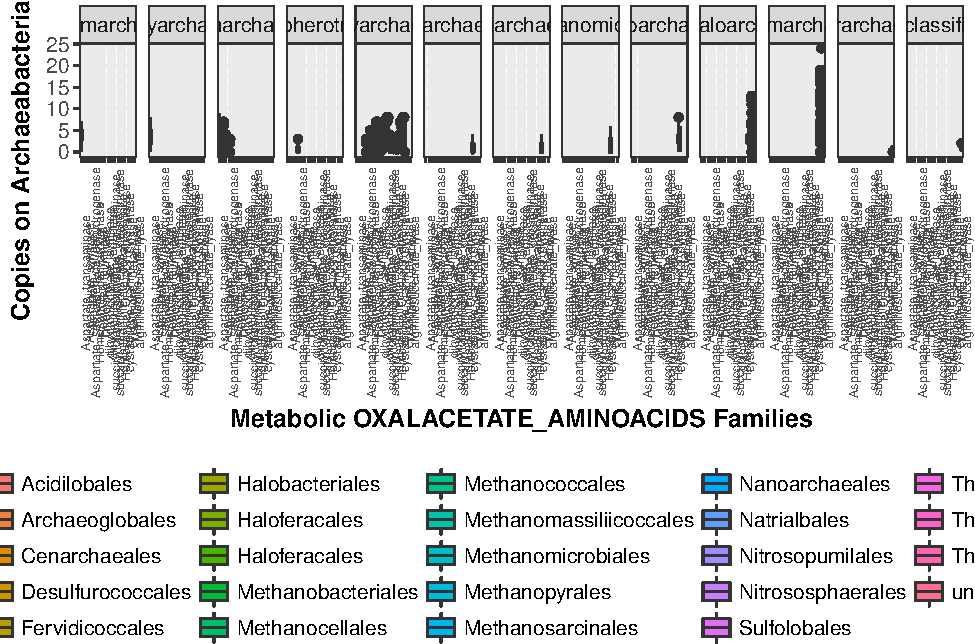
\includegraphics{tesis_files/figure-latex/ArcheaeBoxPlotByPhylum-6} \end{center}
  
  \begin{Shaded}
  \begin{Highlighting}[]
  \CommentTok{#+ geom_jitter(aes(color=MetFam_BP.m$Phylum))}
  
  \NormalTok{MetFam=}\KeywordTok{subset}\NormalTok{(ArchaeasCentral,Pathway==}\StringTok{"R5P_AMINOACIDS"}\NormalTok{)}
  \NormalTok{MetFam_BP.m=ArchaeasHeatPlotBP.m[ArchaeasHeatPlotBP.m$variable %in%}\StringTok{ }\NormalTok{MetFam$Enzyme,]}
  \KeywordTok{ggplot}\NormalTok{(MetFam_BP.m, }\KeywordTok{aes}\NormalTok{(}\DataTypeTok{x=}\NormalTok{MetFam_BP.m$variable, }\DataTypeTok{y=}\NormalTok{MetFam_BP.m$value, }\DataTypeTok{fill=}\NormalTok{Order))+}\StringTok{ }\KeywordTok{labs}\NormalTok{(}\DataTypeTok{x =} \StringTok{"Metabolic R5P_AMINOACIDS Families"}\NormalTok{, }\DataTypeTok{y =} \StringTok{"Copies on Archaeabacteria Genomes"}\NormalTok{,}\DataTypeTok{text =} \KeywordTok{element_text}\NormalTok{(}\DataTypeTok{size=}\DecValTok{12}\NormalTok{)) +}\StringTok{ }\KeywordTok{geom_boxplot}\NormalTok{() +}\StringTok{ }\KeywordTok{facet_grid}\NormalTok{(. ~}\StringTok{ }\NormalTok{Phylum)+}\KeywordTok{theme_bw}\NormalTok{()+}\KeywordTok{theme}\NormalTok{(}\DataTypeTok{plot.title =} \KeywordTok{element_text}\NormalTok{(}\DataTypeTok{size =} \DecValTok{14}\NormalTok{, }\DataTypeTok{face =} \StringTok{"bold"}\NormalTok{), }\DataTypeTok{text =} \KeywordTok{element_text}\NormalTok{(}\DataTypeTok{size =} \DecValTok{12}\NormalTok{), }\DataTypeTok{axis.title =} \KeywordTok{element_text}\NormalTok{(}\DataTypeTok{face=}\StringTok{"bold"}\NormalTok{), }\DataTypeTok{axis.text.x=}\KeywordTok{element_text}\NormalTok{(}\DataTypeTok{angle =} \DecValTok{90}\NormalTok{,}\DataTypeTok{size =} \DecValTok{6}\NormalTok{), }\DataTypeTok{legend.position =} \StringTok{"bottom"}\NormalTok{)}
  \end{Highlighting}
  \end{Shaded}
  
  \begin{center}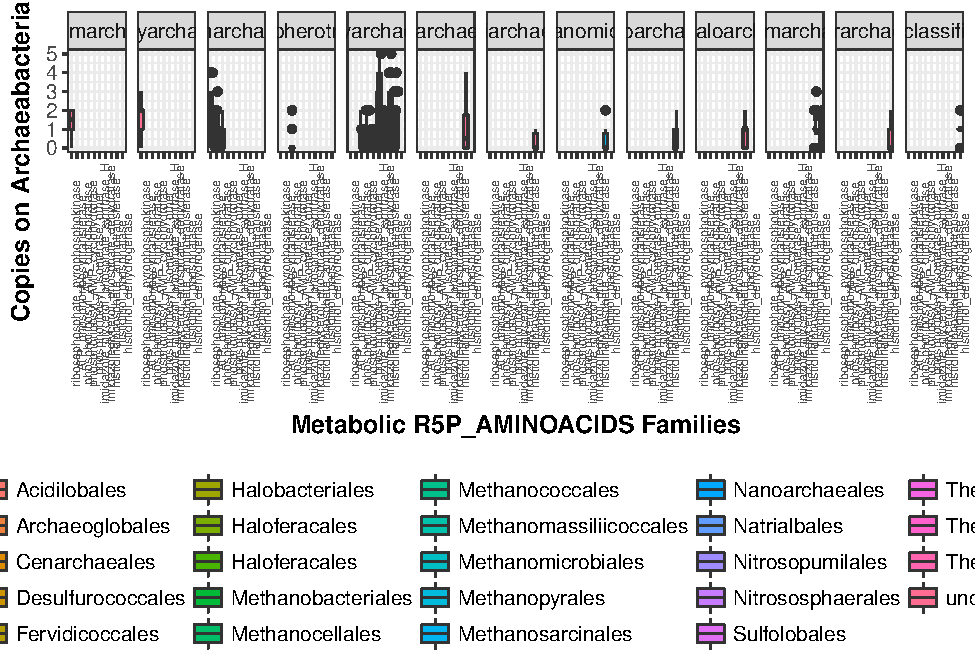
\includegraphics{tesis_files/figure-latex/ArcheaeBoxPlotByPhylum-7} \end{center}
  
  \begin{Shaded}
  \begin{Highlighting}[]
   \CommentTok{#+ geom_jitter(aes(color=MetFam_BP.m$Phylum))}
  
  \CommentTok{#}
  \NormalTok{MetFam=}\KeywordTok{subset}\NormalTok{(ArchaeasCentral,Pathway==}\StringTok{"TCA"}\NormalTok{)}
  \NormalTok{MetFam_BP.m=ArchaeasHeatPlotBP.m[ArchaeasHeatPlotBP.m$variable %in%}\StringTok{ }\NormalTok{MetFam$Enzyme,]}
  \KeywordTok{ggplot}\NormalTok{(MetFam_BP.m, }\KeywordTok{aes}\NormalTok{(}\DataTypeTok{x=}\NormalTok{MetFam_BP.m$variable, }\DataTypeTok{y=}\NormalTok{MetFam_BP.m$value, }\DataTypeTok{fill=}\NormalTok{Order))+}\StringTok{ }\KeywordTok{labs}\NormalTok{(}\DataTypeTok{x =} \StringTok{"Metabolic TCA Families"}\NormalTok{, }\DataTypeTok{y =} \StringTok{"Copies on Archaeabacteria Genomes"}\NormalTok{,}\DataTypeTok{text =} \KeywordTok{element_text}\NormalTok{(}\DataTypeTok{size=}\DecValTok{12}\NormalTok{)) +}\StringTok{ }\KeywordTok{geom_boxplot}\NormalTok{() +}\StringTok{ }\KeywordTok{facet_grid}\NormalTok{(. ~}\StringTok{ }\NormalTok{Phylum)+}\KeywordTok{theme_bw}\NormalTok{() +}\KeywordTok{theme}\NormalTok{(}\DataTypeTok{plot.title =} \KeywordTok{element_text}\NormalTok{(}\DataTypeTok{size =} \DecValTok{14}\NormalTok{, }\DataTypeTok{face =} \StringTok{"bold"}\NormalTok{), }\DataTypeTok{text =} \KeywordTok{element_text}\NormalTok{(}\DataTypeTok{size =} \DecValTok{12}\NormalTok{), }\DataTypeTok{axis.title =} \KeywordTok{element_text}\NormalTok{(}\DataTypeTok{face=}\StringTok{"bold"}\NormalTok{), }\DataTypeTok{axis.text.x=}\KeywordTok{element_text}\NormalTok{(}\DataTypeTok{angle =} \DecValTok{90}\NormalTok{,}\DataTypeTok{size =} \DecValTok{6}\NormalTok{), }\DataTypeTok{legend.position =} \StringTok{"bottom"}\NormalTok{)}
  \end{Highlighting}
  \end{Shaded}
  
  \begin{center}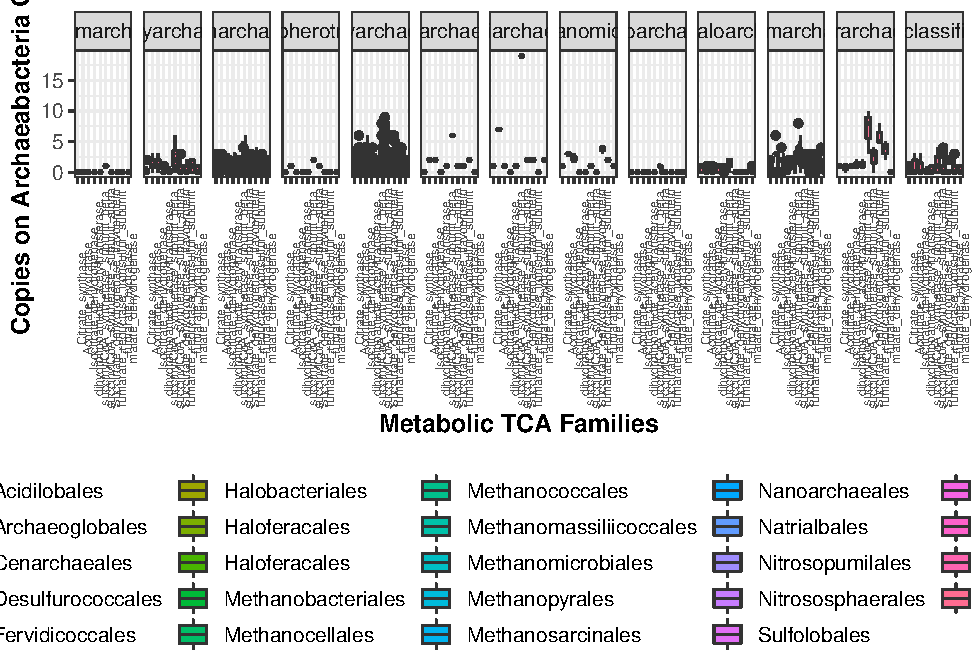
\includegraphics{tesis_files/figure-latex/ArcheaeBoxPlotByPhylum-8} \end{center}
  
  \begin{Shaded}
  \begin{Highlighting}[]
  \CommentTok{#+ geom_jitter(aes(color=MetFam_BP.m$Phylum))}
  
  \NormalTok{MetFam=}\KeywordTok{subset}\NormalTok{(ArchaeasCentral,Pathway==}\StringTok{"E4P_AMINO_ACIDS"}\NormalTok{)}
  \NormalTok{MetFam_BP.m=ArchaeasHeatPlotBP.m[ArchaeasHeatPlotBP.m$variable %in%}\StringTok{ }\NormalTok{MetFam$Enzyme,]}
  \KeywordTok{ggplot}\NormalTok{(MetFam_BP.m, }\KeywordTok{aes}\NormalTok{(}\DataTypeTok{x=}\NormalTok{MetFam_BP.m$variable, }\DataTypeTok{y=}\NormalTok{MetFam_BP.m$value, }\DataTypeTok{fill=}\NormalTok{Order))+}\StringTok{ }\KeywordTok{labs}\NormalTok{(}\DataTypeTok{x =} \StringTok{"Metabolic E4P_AMINO_ACIDS Families"}\NormalTok{, }\DataTypeTok{y =} \StringTok{"Copies on Archaeabacteria Genomes"}\NormalTok{,}\DataTypeTok{text =} \KeywordTok{element_text}\NormalTok{(}\DataTypeTok{size=}\DecValTok{12}\NormalTok{)) +}\StringTok{ }\KeywordTok{geom_boxplot}\NormalTok{() +}\StringTok{ }\KeywordTok{facet_grid}\NormalTok{(. ~}\StringTok{ }\NormalTok{Phylum)+}\KeywordTok{theme_bw}\NormalTok{() +}\KeywordTok{theme}\NormalTok{(}\DataTypeTok{plot.title =} \KeywordTok{element_text}\NormalTok{(}\DataTypeTok{size =} \DecValTok{14}\NormalTok{, }\DataTypeTok{face =} \StringTok{"bold"}\NormalTok{), }\DataTypeTok{text =} \KeywordTok{element_text}\NormalTok{(}\DataTypeTok{size =} \DecValTok{12}\NormalTok{), }\DataTypeTok{axis.title =} \KeywordTok{element_text}\NormalTok{(}\DataTypeTok{face=}\StringTok{"bold"}\NormalTok{), }\DataTypeTok{axis.text.x=}\KeywordTok{element_text}\NormalTok{(}\DataTypeTok{angle =} \DecValTok{90}\NormalTok{,}\DataTypeTok{size =} \DecValTok{6}\NormalTok{), }\DataTypeTok{legend.position =} \StringTok{"bottom"}\NormalTok{)}
  \end{Highlighting}
  \end{Shaded}
  
  \begin{center}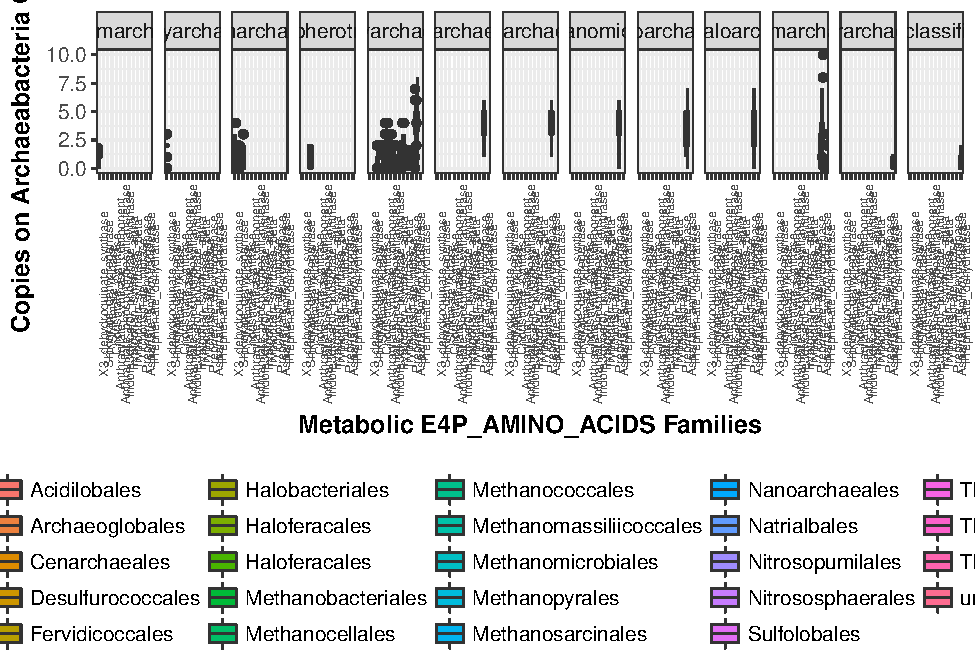
\includegraphics{tesis_files/figure-latex/ArcheaeBoxPlotByPhylum-9} \end{center}
  
  \begin{Shaded}
  \begin{Highlighting}[]
  \CommentTok{#+ geom_jitter(aes(color=MetFam_BP.m$Phylum))}
  
  
  \NormalTok{MetFam=}\KeywordTok{subset}\NormalTok{(ArchaeasCentral,Pathway==}\StringTok{"PYR_THR_AA"}\NormalTok{)}
  \NormalTok{MetFam_BP.m=ArchaeasHeatPlotBP.m[ArchaeasHeatPlotBP.m$variable %in%}\StringTok{ }\NormalTok{MetFam$Enzyme,]}
  \KeywordTok{ggplot}\NormalTok{(MetFam_BP.m, }\KeywordTok{aes}\NormalTok{(}\DataTypeTok{x=}\NormalTok{MetFam_BP.m$variable, }\DataTypeTok{y=}\NormalTok{MetFam_BP.m$value, }\DataTypeTok{fill=}\NormalTok{Order))+}\StringTok{ }\KeywordTok{labs}\NormalTok{(}\DataTypeTok{x =} \StringTok{"Metabolic Families on PYR_THR_AA pathway "}\NormalTok{, }\DataTypeTok{y =} \StringTok{"Copies on Archaeabacteria Genomes"}\NormalTok{,}\DataTypeTok{text =} \KeywordTok{element_text}\NormalTok{(}\DataTypeTok{size=}\DecValTok{12}\NormalTok{)) +}\StringTok{ }\KeywordTok{geom_boxplot}\NormalTok{() +}\StringTok{ }\KeywordTok{facet_grid}\NormalTok{(. ~}\StringTok{ }\NormalTok{Phylum)+}\KeywordTok{theme_bw}\NormalTok{() +}\KeywordTok{theme}\NormalTok{(}\DataTypeTok{plot.title =} \KeywordTok{element_text}\NormalTok{(}\DataTypeTok{size =} \DecValTok{14}\NormalTok{, }\DataTypeTok{face =} \StringTok{"bold"}\NormalTok{), }\DataTypeTok{text =} \KeywordTok{element_text}\NormalTok{(}\DataTypeTok{size =} \DecValTok{12}\NormalTok{), }\DataTypeTok{axis.title =} \KeywordTok{element_text}\NormalTok{(}\DataTypeTok{face=}\StringTok{"bold"}\NormalTok{), }\DataTypeTok{axis.text.x=}\KeywordTok{element_text}\NormalTok{(}\DataTypeTok{angle =} \DecValTok{90}\NormalTok{,}\DataTypeTok{size =} \DecValTok{6}\NormalTok{), }\DataTypeTok{legend.position =} \StringTok{"bottom"}\NormalTok{)}
  \end{Highlighting}
  \end{Shaded}
  
  \begin{center}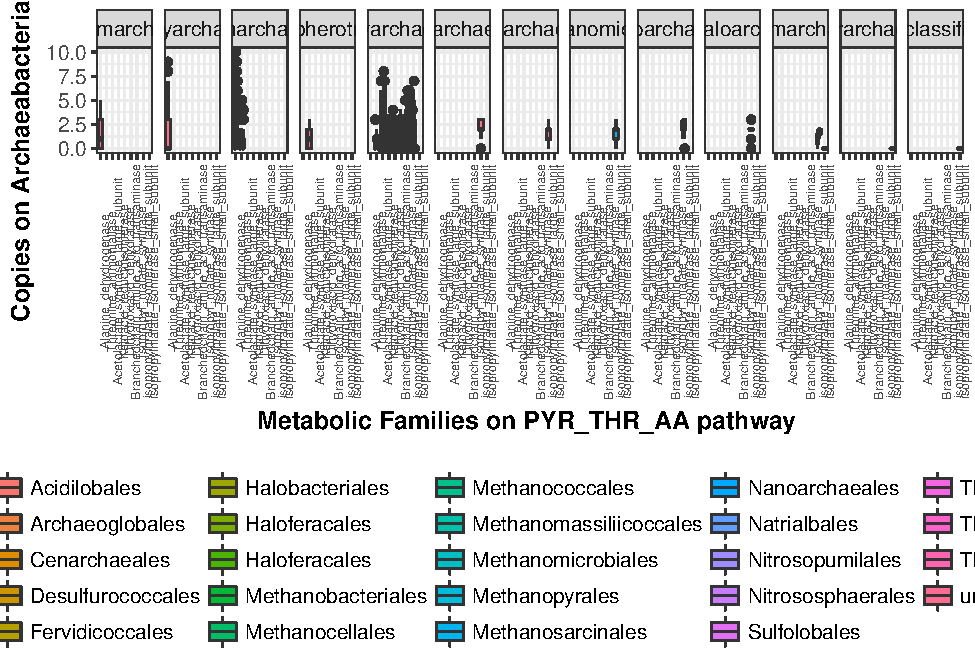
\includegraphics{tesis_files/figure-latex/ArcheaeBoxPlotByPhylum-10} \end{center}
  
  \begin{Shaded}
  \begin{Highlighting}[]
  \CommentTok{#+ geom_jitter(aes(color=MetFam_BP.m$Phylum))}
  
  \CommentTok{#ggsave("chapter3/expansion_plotArchaeas.pdf", plot = expansion_plotArchaea,height = 8, width = 7)}
  \end{Highlighting}
  \end{Shaded}
  
  \clearpage 
  
  \section{Central pathway expansions}\label{central-pathway-expansions}
  
  Heat plot of central pathways expansions, Needs to be phylogenetically
  sorted.
  
  \begin{figure}[h!tbp]
  \centering
  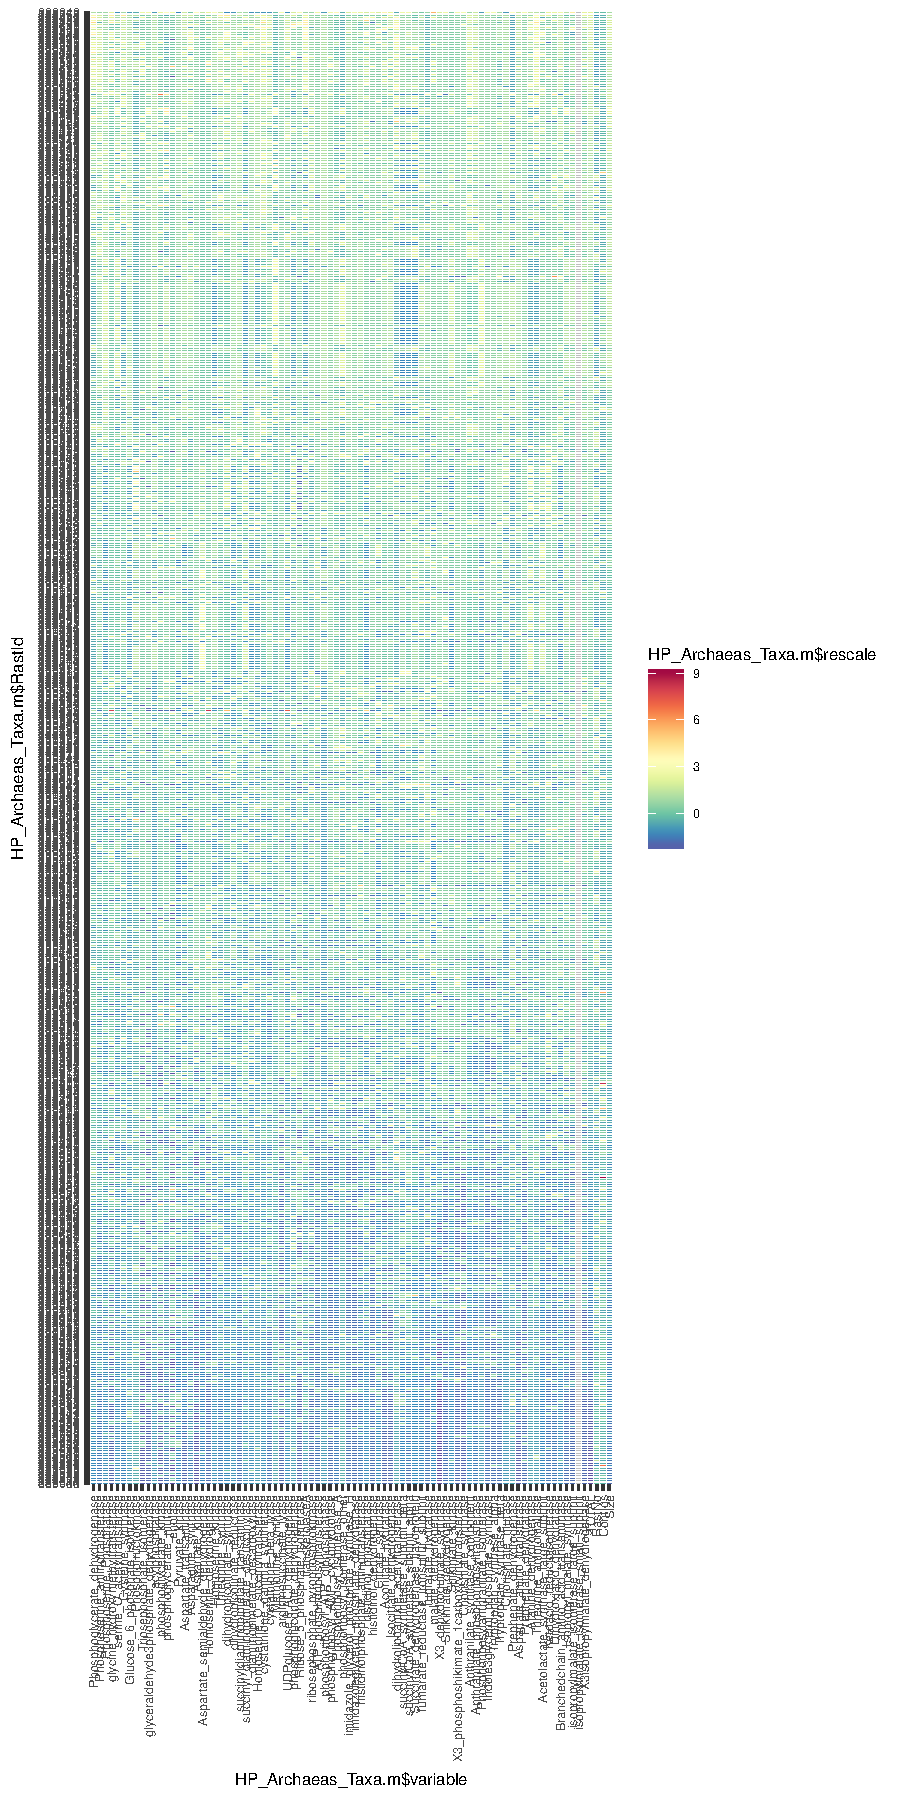
\includegraphics[angle = 0,scale = 0.6]{chapter3/ArchaeasHeatPlot.pdf}
  \caption[Archaeas Heatplot]{\normalsize{Archaeas Heatplot}}
  \label{fig:ArchaeaPlot}
  \end{figure}
  
  Here is a reference to the HeatPlot: \autoref{fig:ArchaeaPlot}.
  \clearpage 
  
  \section{Genome Size correlations}\label{genome-size-correlations}
  
  \subsection{Correlation between genome size and AntiSMASH
  products}\label{correlation-between-genome-size-and-antismash-products}
  
  Genome size vs Total antismash cluster coloured by order
  
  \begin{figure}[h!tbp]
  \centering
  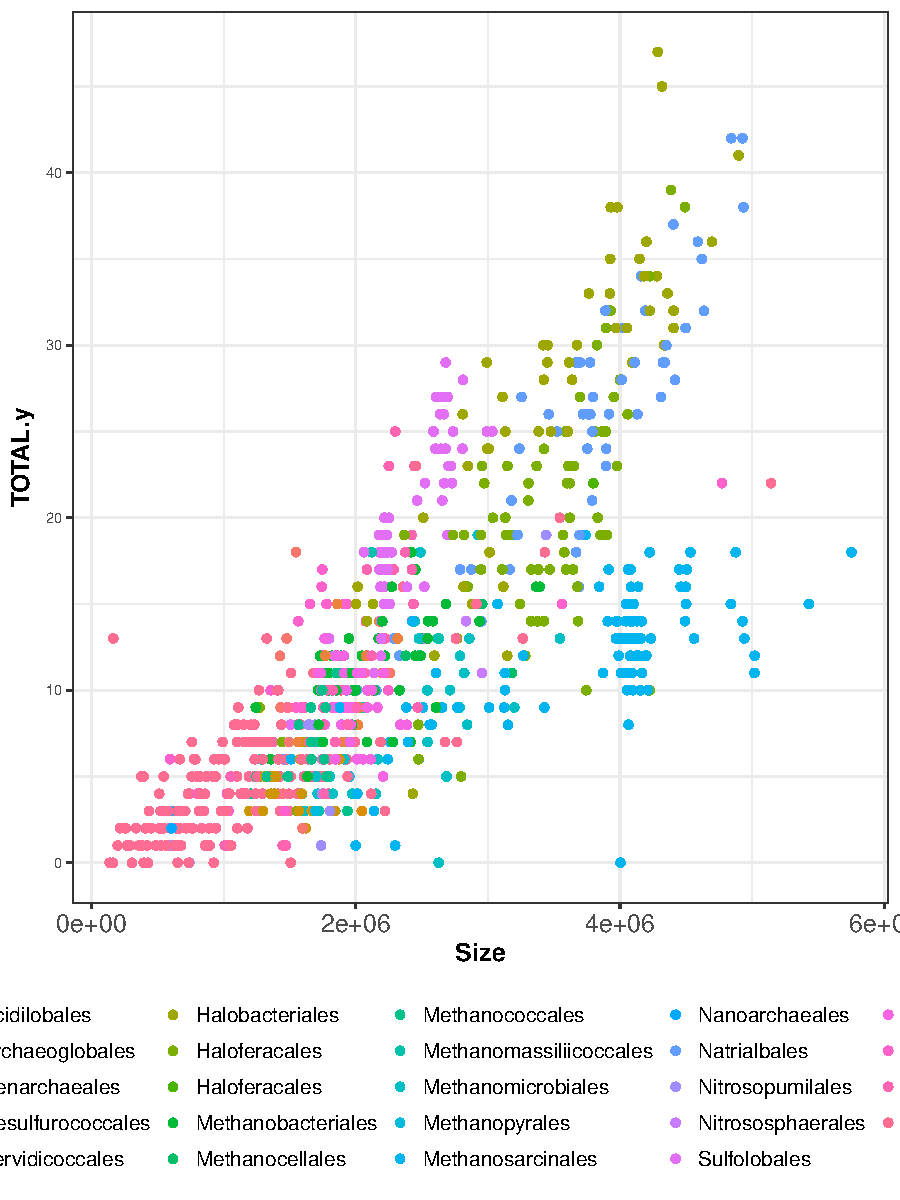
\includegraphics[angle = 0,scale = 0.6]{chapter3/ArchaeasSMASHvsSizebyOrder.pdf}
  \caption[Correlation between Archaeas genome size and antismash Natural products detection colored by Order]{\normalsize{Correlation between Archaeas genome size and antismash Natural products detection colored by Order}}
  \label{fig:ArchaeasSMASHvsSizebyOrder}
  \end{figure}
  
  Here is a reference to Genome size vs Total antismash cluster:
  \autoref{fig:ArchaeasSMASHvsSizebyOrder}. \clearpage
  
  Genome size vs Total antismash cluster detected splitted by order
  
  \begin{figure}[h!tbp]
  \centering
  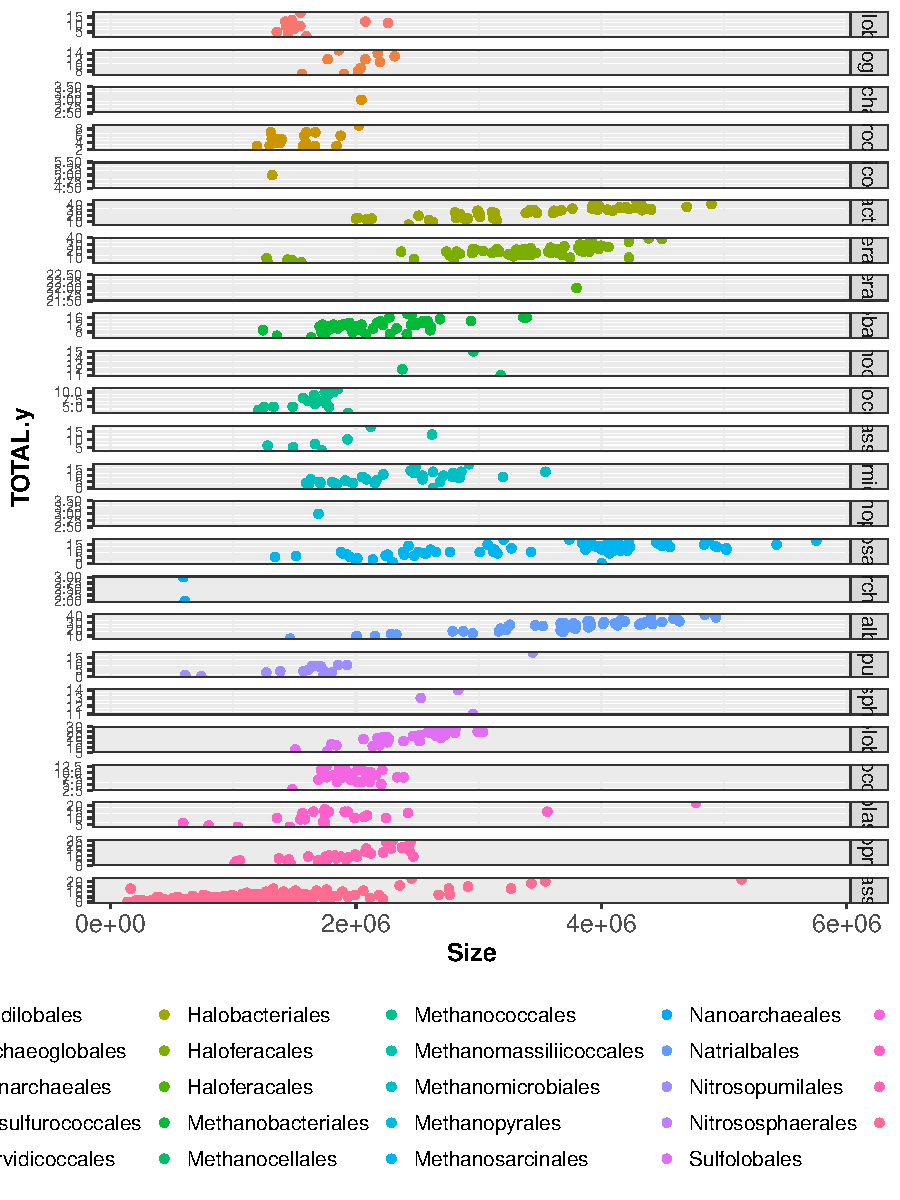
\includegraphics[angle = 0,scale = 0.6]{chapter3/ArchaeasSMASHvsSizeGridOrder.pdf}
  \caption[Correlation between Archaeas genome size and antismash Natural products detection grided by Order]{\normalsize{Correlation between Archaeas genome size and antismash Natural products detection grided by Order}}
  \label{fig:ArchaeasSMASHvsSizeGridOrder}
  \end{figure}
  
  Here is a reference to Correlation between genome size and antismash
  Natural products detection grided by Order plot:
  \autoref{fig:ArchaeasSMASHvsSizeGridOrder}. \clearpage 
  
  \subsection{Correlation between genome size and Central pathway
  expansions}\label{correlation-between-genome-size-and-central-pathway-expansions}
  
  Genome size vs Total central pathway expansion coloured by order
  
  \begin{figure}[h!tbp]
  \centering
  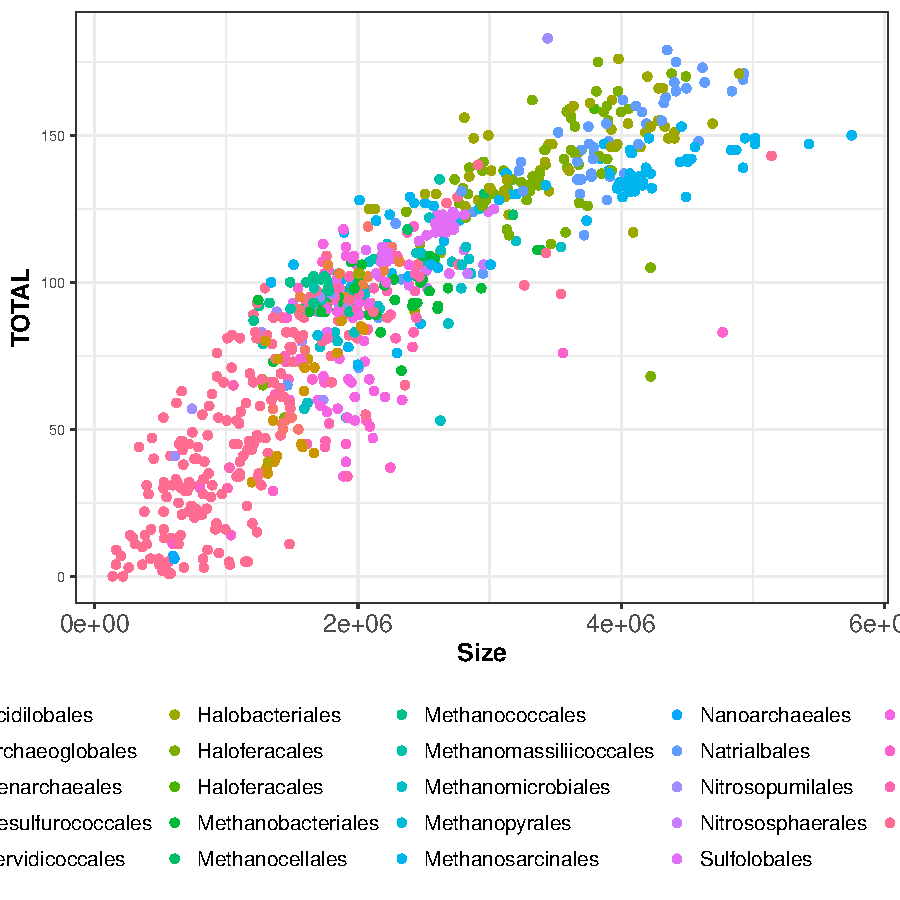
\includegraphics[angle = 0,scale = 1]{chapter3/ArchaeasSizevsExpansionsbyOrder.pdf}
  \caption[Correlation between Archaeas genome size and central pathway expansions ]{\normalsize{Correlation between Archaeas genome size and central pathway expansions }}
  \label{fig:ArchaeasSizevsExpansionsbyOrder}
  \end{figure}
  
  Here is a reference to the size vs Total central pathway expansion plot:
  \autoref{fig:ArchaeasSizevsExpansionsbyOrder}. \clearpage 
  
  Genome size vs Total central pathway expansion grided by order
  
  \begin{figure}[h!tbp]
  \centering
  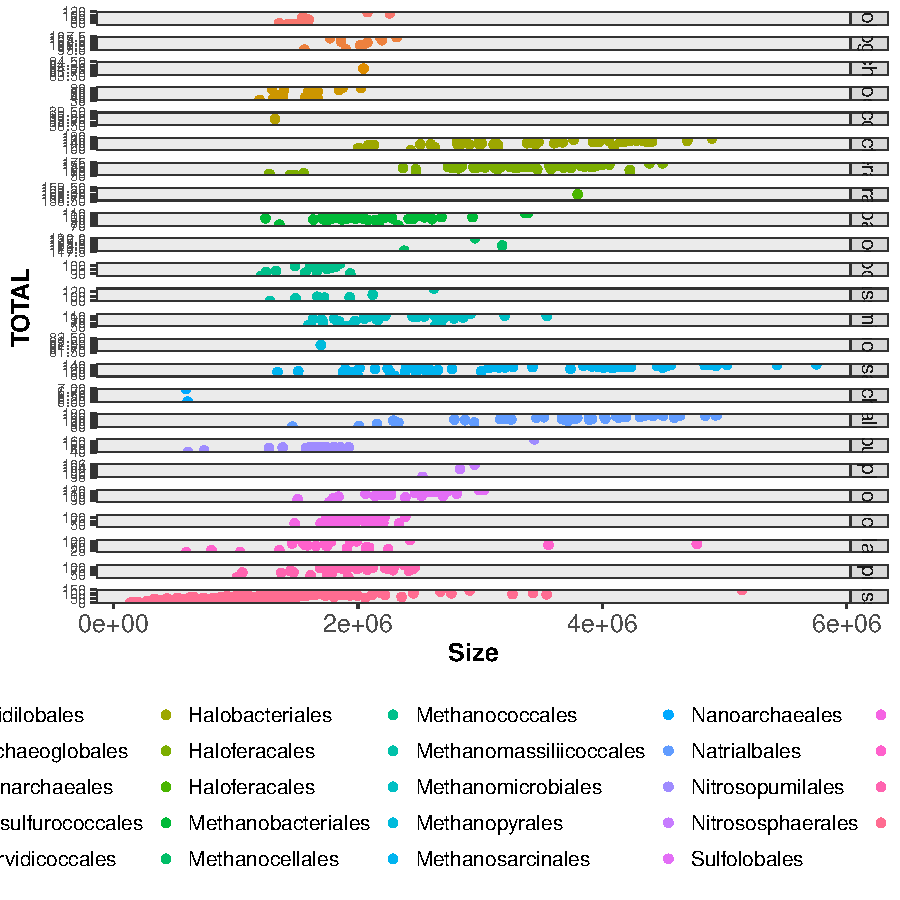
\includegraphics[angle = 0,scale = 1]{chapter3/ArchaeasSizevsExpansionsGridbyOrder.pdf}
  \caption[Correlation between Archaeas genome size and central pathway expansions grided by order]{\normalsize{Correlation between Archaeas genome size and central pathway expansions grided by order}}
  \label{fig:ArchaeasSizevsExpansionsGridbyOrder}
  \end{figure}
  
  Here is a reference to the Genome size vs Total central pathway
  expansion grided by order plot:
  \autoref{fig:ArchaeasSizevsExpansionsGridbyOrder}. \clearpage 
  
  Correlation between genome size and each of the central pathway
  families. Data are coloured by metabolic family instead of coloured by
  taxonomical order. This treatment allows to answer how differente
  metabolic families grows when genome size grow.\\
  Also I want to add form given by taxonomical order.
  
  \begin{verbatim}
  Warning: The shape palette can deal with a maximum of 6 discrete values
  because more than 6 becomes difficult to discriminate; you have
  24. Consider specifying shapes manually if you must have them.
  \end{verbatim}
  
  \begin{verbatim}
  Warning: Removed 64823 rows containing missing values (geom_point).
  \end{verbatim}
  
  Genome size vs Total central pathway expansion coloured by metabolic
  Family
  
  \begin{figure}[h!tbp]
  \centering
  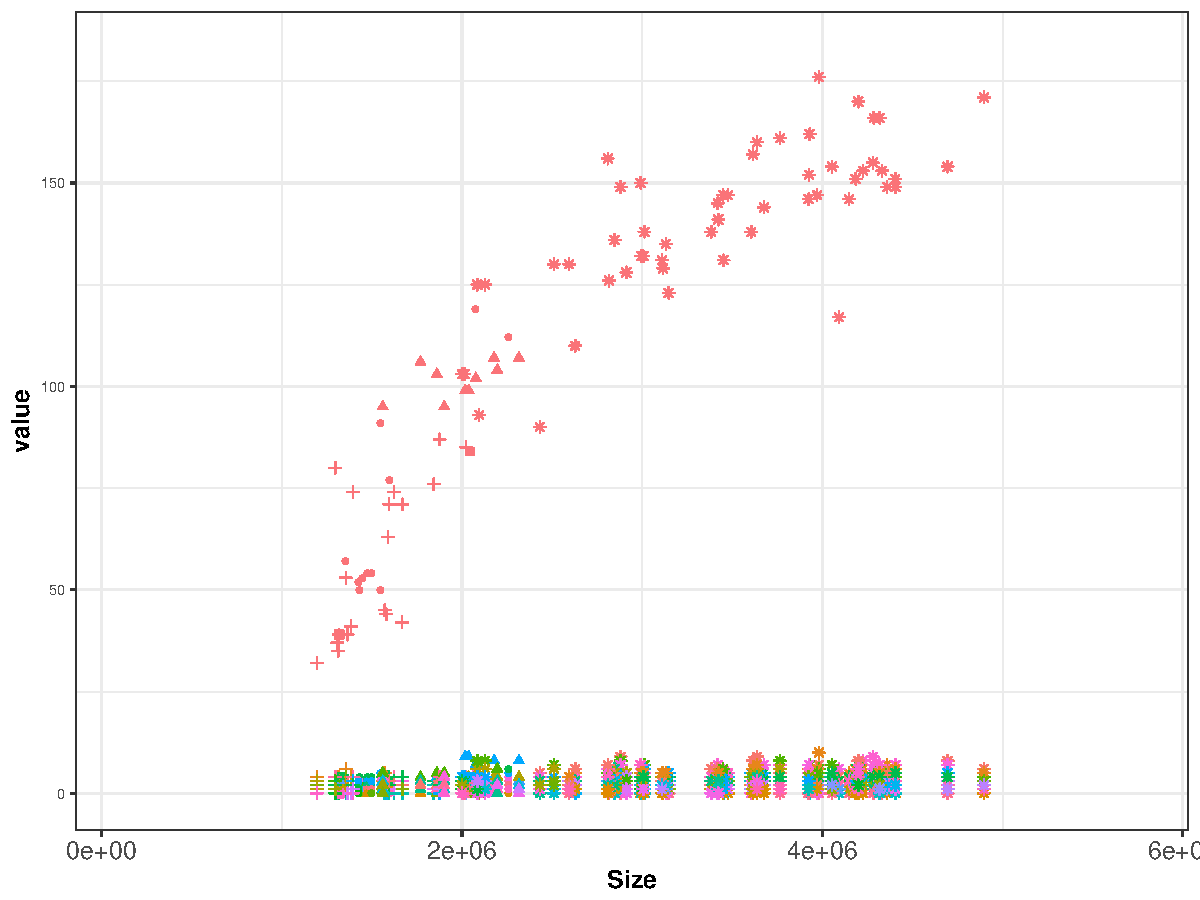
\includegraphics[angle = 0,scale = 0.6]{chapter3/ArchaeasSizevsExpansionsbyMetabolicFamily.pdf}
  \caption[Correlation between Archaeas Genome size vs Total central pathway expansion coloured by metabolic Family]{\normalsize{Correlation between Archaeas Genome size vs Total central pathway expansion coloured by metabolic Family}}
  \label{fig:ArchaeasSizevsExpansionsbyMetabolicFamily}
  \end{figure}
  
  Here is a reference to the Genome size vs Total central pathway
  expansion coloured by metabolic Family plot:
  \autoref{fig:ArchaeasSizevsExpansionsbyMetabolicFamily}. \clearpage 
  
  Future Work: Genome size vs Total central pathway expansion grided by
  metabolic Family For clarity I need to also grid and group by Metabolic
  Pathway
  
  Here is a reference to Genome size vs Total central pathway expansion
  grided by metabolic Family plot:
  \autoref{fig:ArchaeasExpansionsbyMetabolicFamilyGrid}. \clearpage 
  
  \section{Natural products}\label{natural-products}
  
  \subsection{Natural products recruitments from EvoMining
  heatplot}\label{natural-products-recruitments-from-evomining-heatplot}
  
  We can see natural products recruitment after central pathways
  expansions colored by their kingdom.\\
  Natural products recruited by metabolic family, colored by phylogenetic
  origin.
  
  Recruitments after central pathways expansions coloured by Kingdom
  
  \begin{figure}[h!tbp]
  \centering
  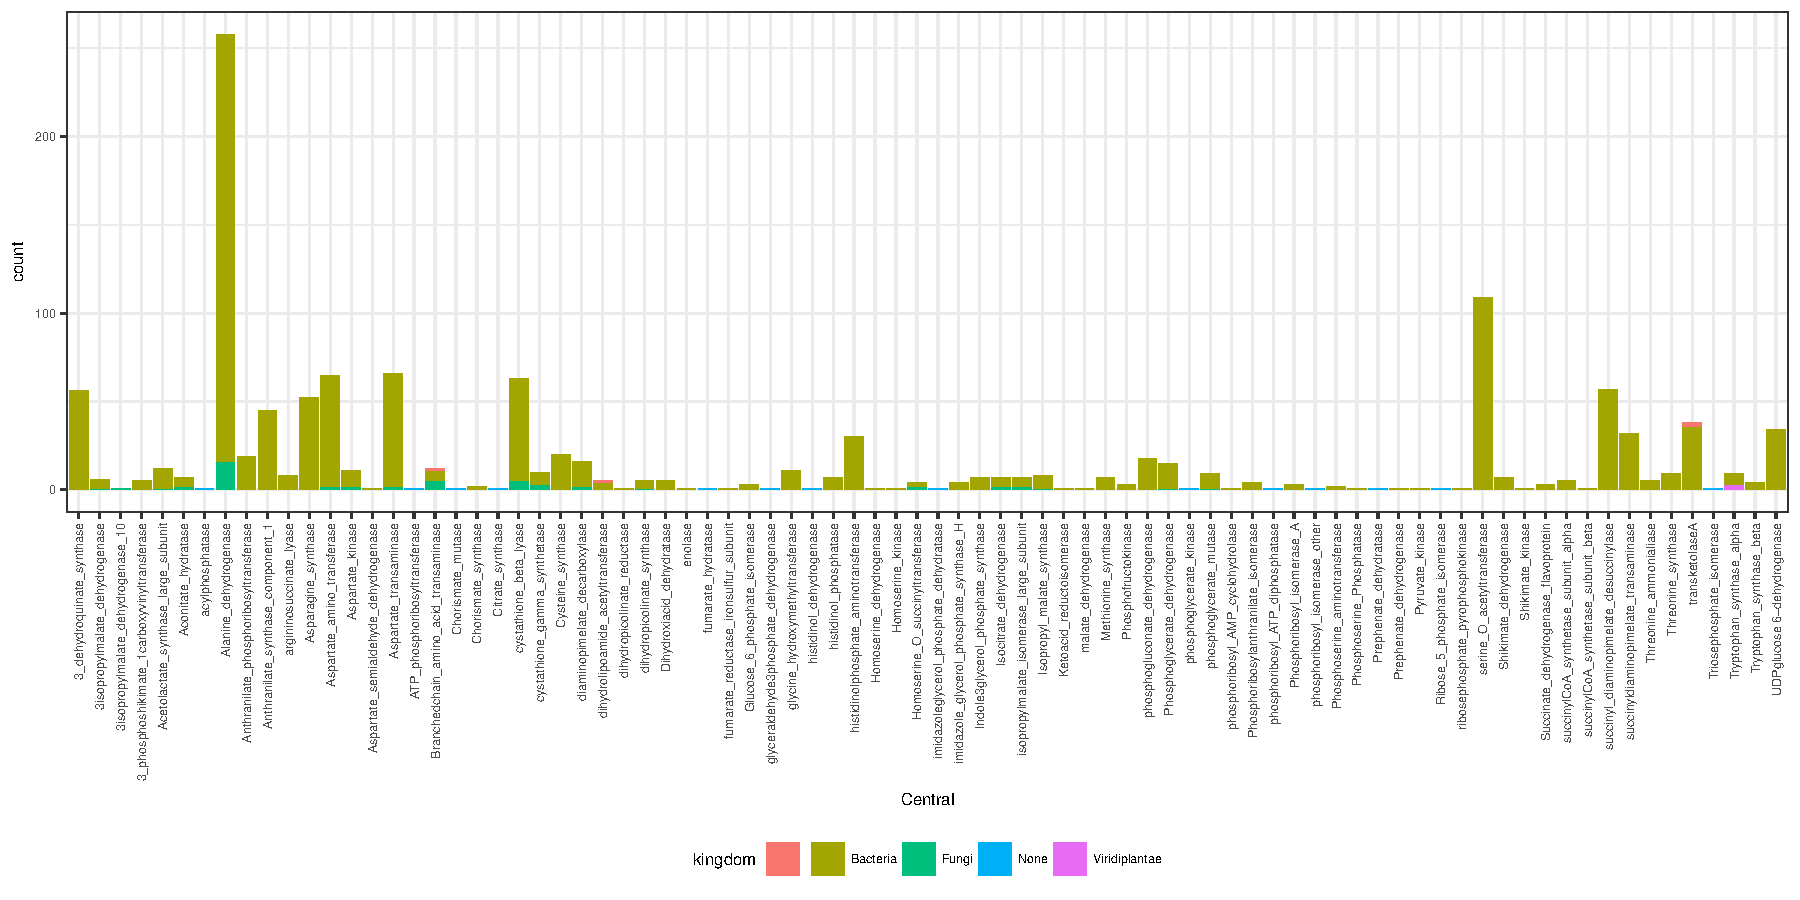
\includegraphics[angle = 0,scale = 0.6]{chapter3/ArchaeasRecruitmentsbyKingdom.pdf}
  \caption[Archaeas Recruitmens on central families coloured by kingdom]{\normalsize{Archaeas Recruitmens on central families coloured by kingdom}}
  \label{fig:ArchaeasRecruitmentsbyKingdom}
  \end{figure}
  
  Here is a reference to Recruitments after central pathways expansions
  colourd by Kingdom plot: \autoref{fig:ArchaeasRecruitmentsbyKingdom}.
  
  \clearpage 
  Recruitments after central pathways expansions colourd by taxonomy
  
  \begin{figure}[h!tbp]
  \centering
  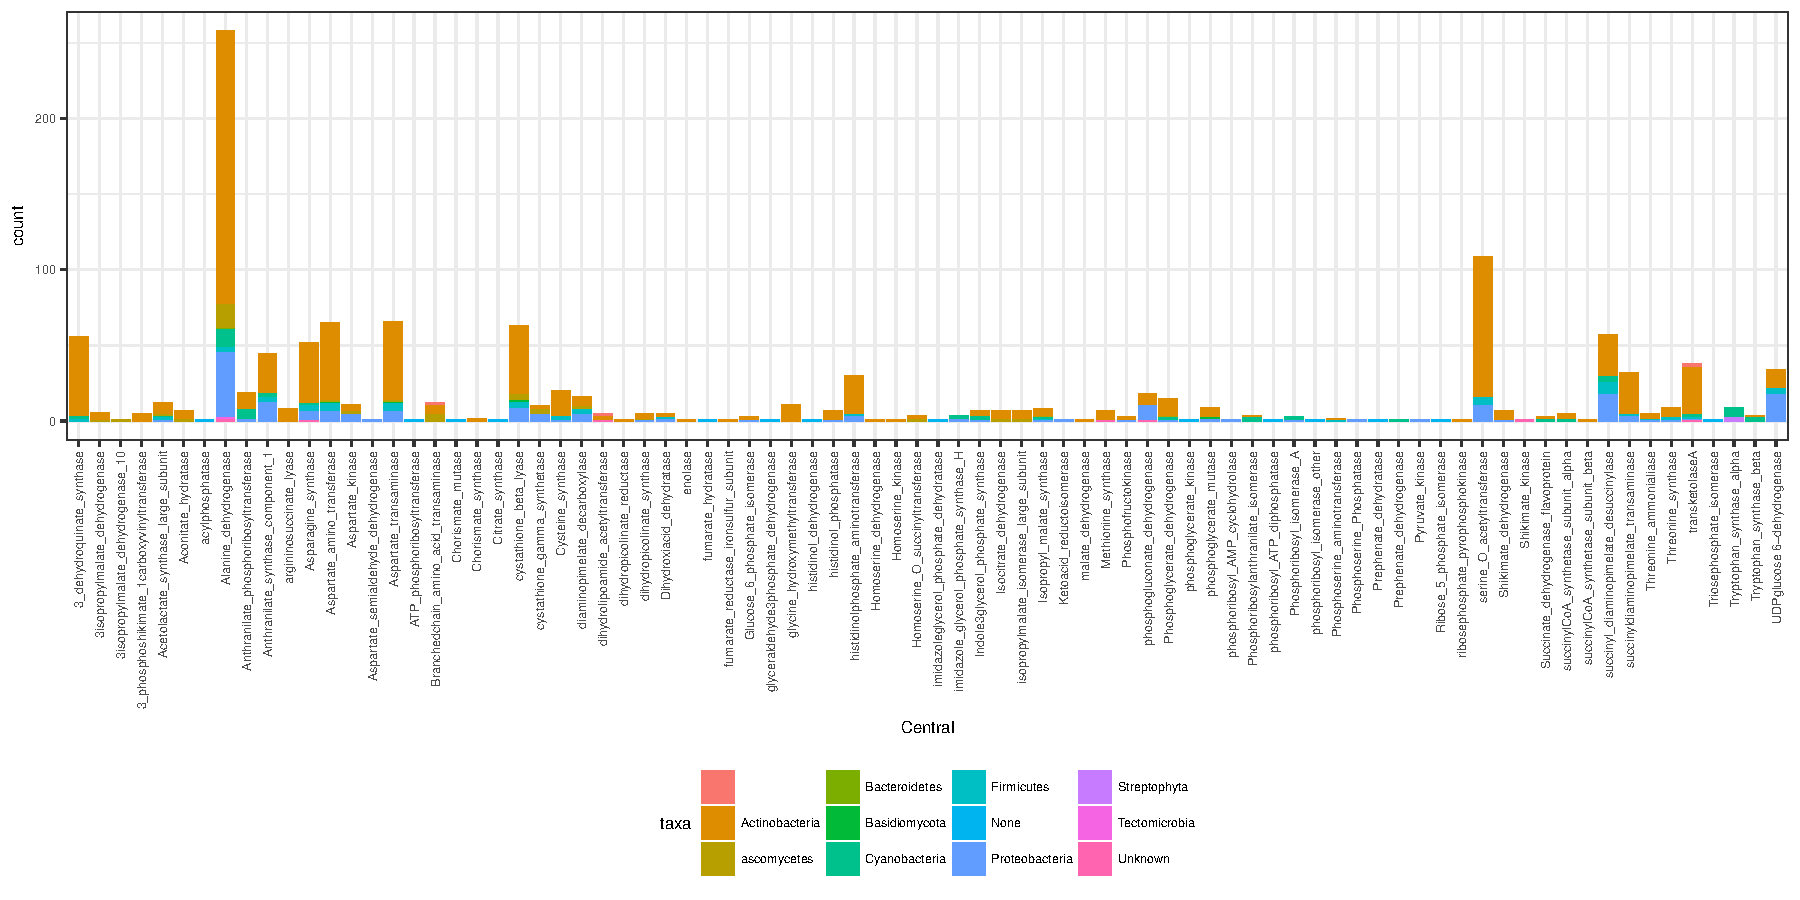
\includegraphics[angle = 0,scale = 0.5]{chapter3/ArchaeasRecruitmentsbyTaxa.pdf}
  \caption[Archaeas Recruitmens on central families coloured by taxonomy]{\normalsize{Archaeas Recruitmens on central families coloured by taxonomy}}
  \label{fig:ArchaeasRecruitmentsbyTaxa}
  \end{figure}
  
  Here is a reference to Recruitments after central pathways expansions
  colourd by taxa plot: \autoref{fig:ArchaeasRecruitmentsbyTaxa}.
  \clearpage 
  
  \section{Archaeas AntiSMASH}\label{archaeas-antismash}
  
  Taxonomical diversity on Archaeasbacteria Data
  
  \begin{figure}[h!tbp]
  \centering
  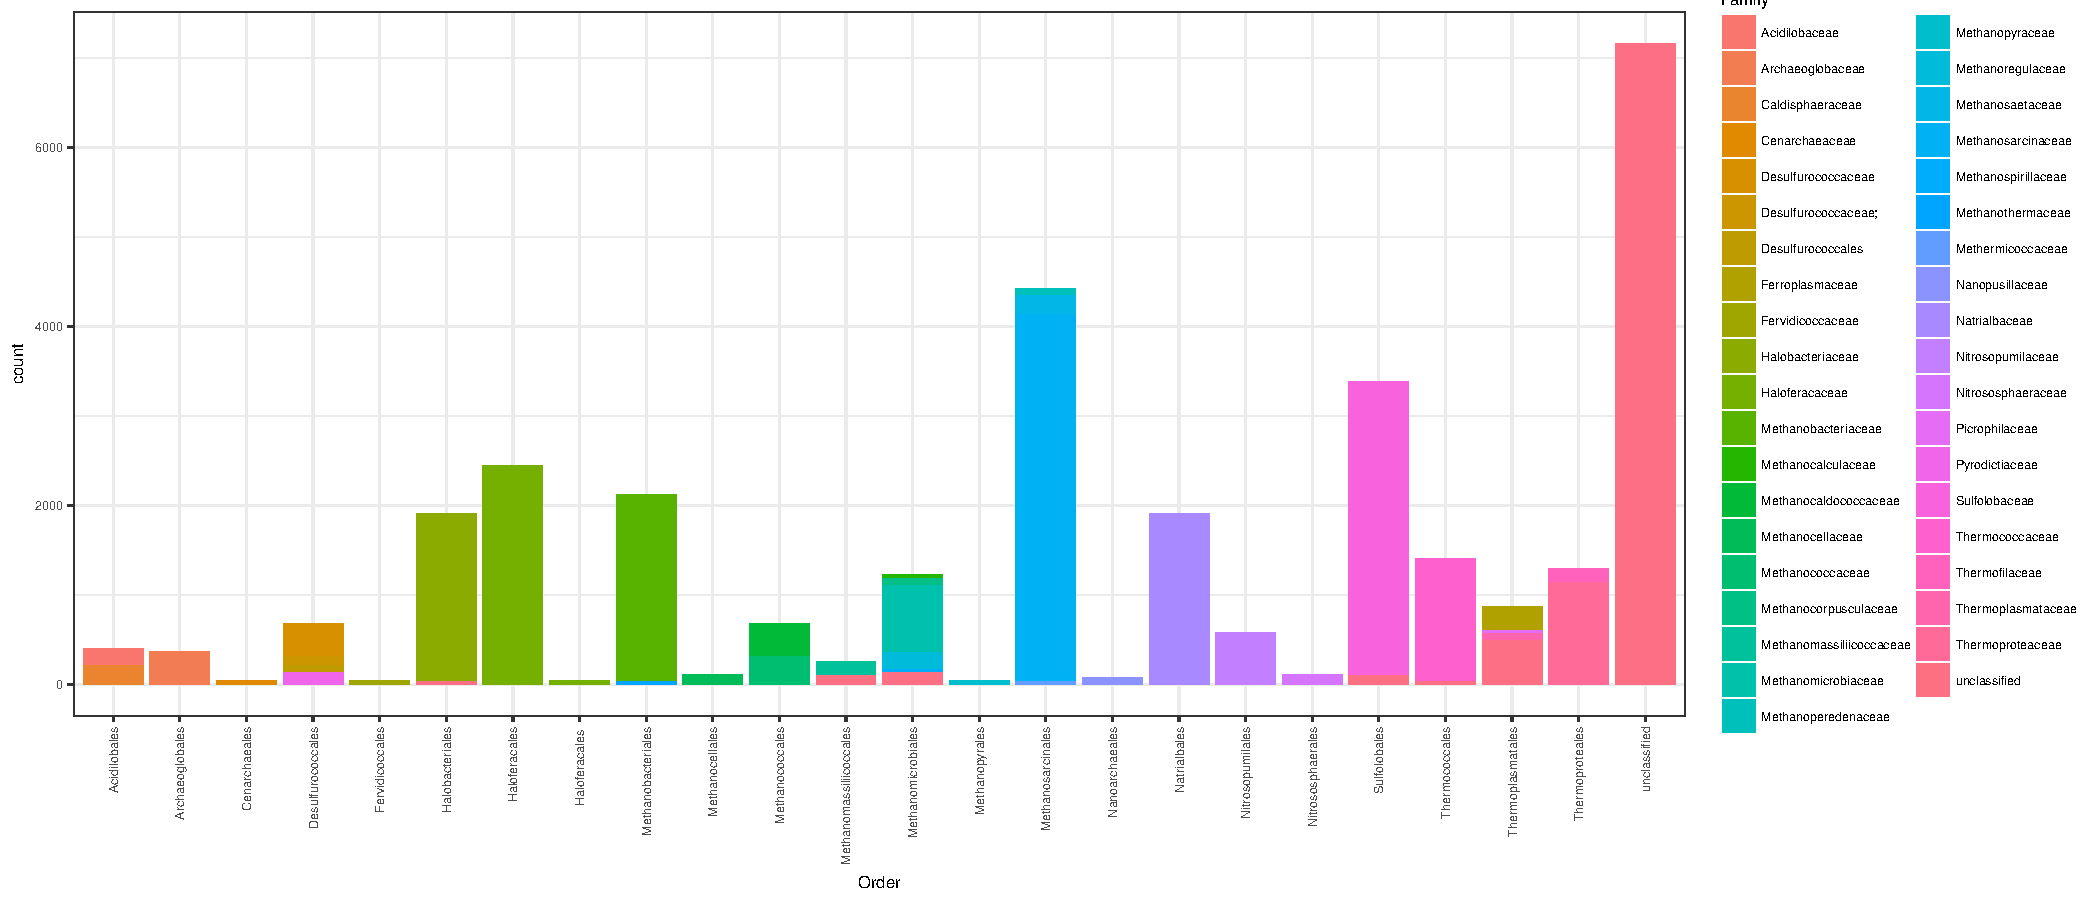
\includegraphics[angle = 0,scale = 0.6]{chapter3/ArchaeasDiversity.pdf}
  \caption[Archaeas Diversity]{\normalsize{Archaeas Diversity}}
  \label{fig:ArchaeasDiversity}
  \end{figure}
  
  Here is a reference to Recruitments after central pathways expansions
  colourd by taxa plot: \autoref{fig:ArchaeasDiversity}. \clearpage
  
  Smash diversity
  
  \begin{figure}[h!tbp]
  \centering
  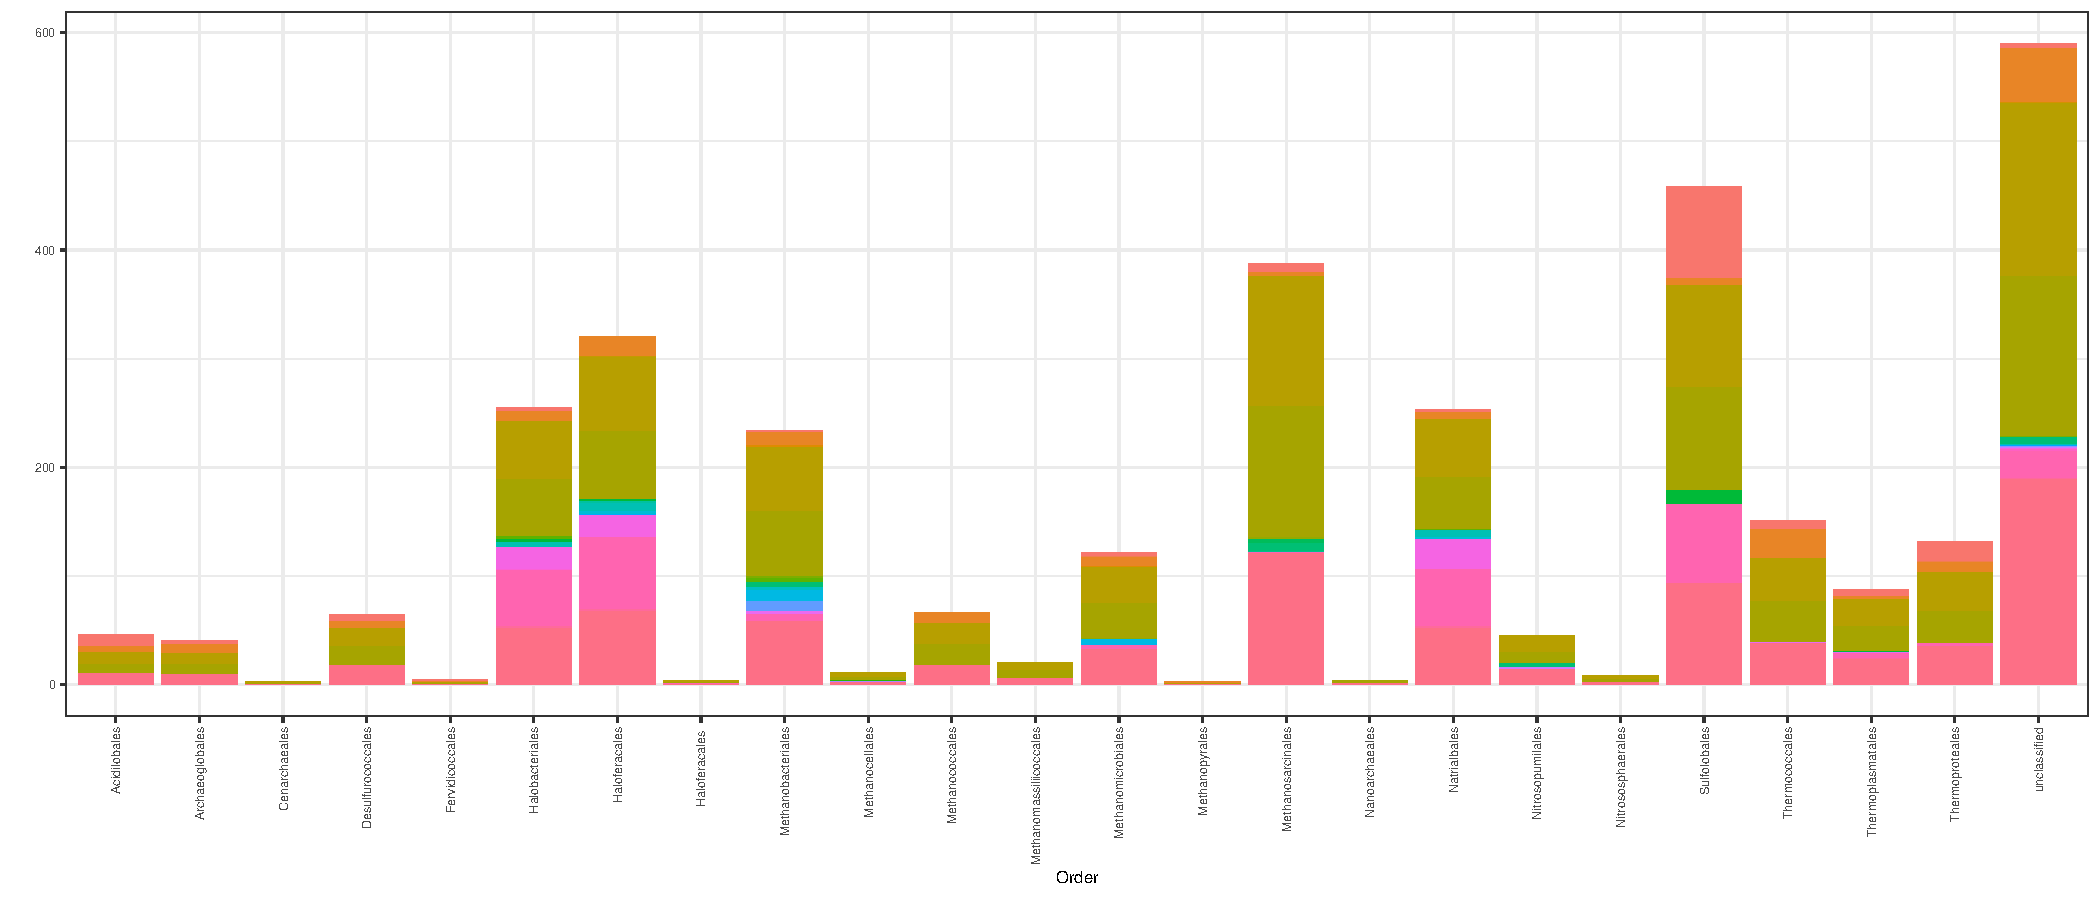
\includegraphics[angle = 0,scale = 0.5]{chapter3/ArchaeasSmash.pdf}
  \caption[Archaeas Smash Taxonomical Diversity]{\normalsize{Archaeas Smash Taxonomical Diversity}}
  \label{fig:ArchaeasSmash}
  \end{figure}
  
  Here is a reference to Recruitments after central pathways expansions
  colourd by taxa plot: \autoref{fig:ArchaeasSmash}. \clearpage
  
  \subsection{AntisSMASH vs Central
  Expansions}\label{antissmash-vs-central-expansions}
  
  Is it a correlation between pangenome grow and central pathways
  expansions?
  
  Total central pathway expansions by genome vs Total antismash cluster
  detected coloured by order
  
  \begin{figure}[h!tbp]
  \centering
  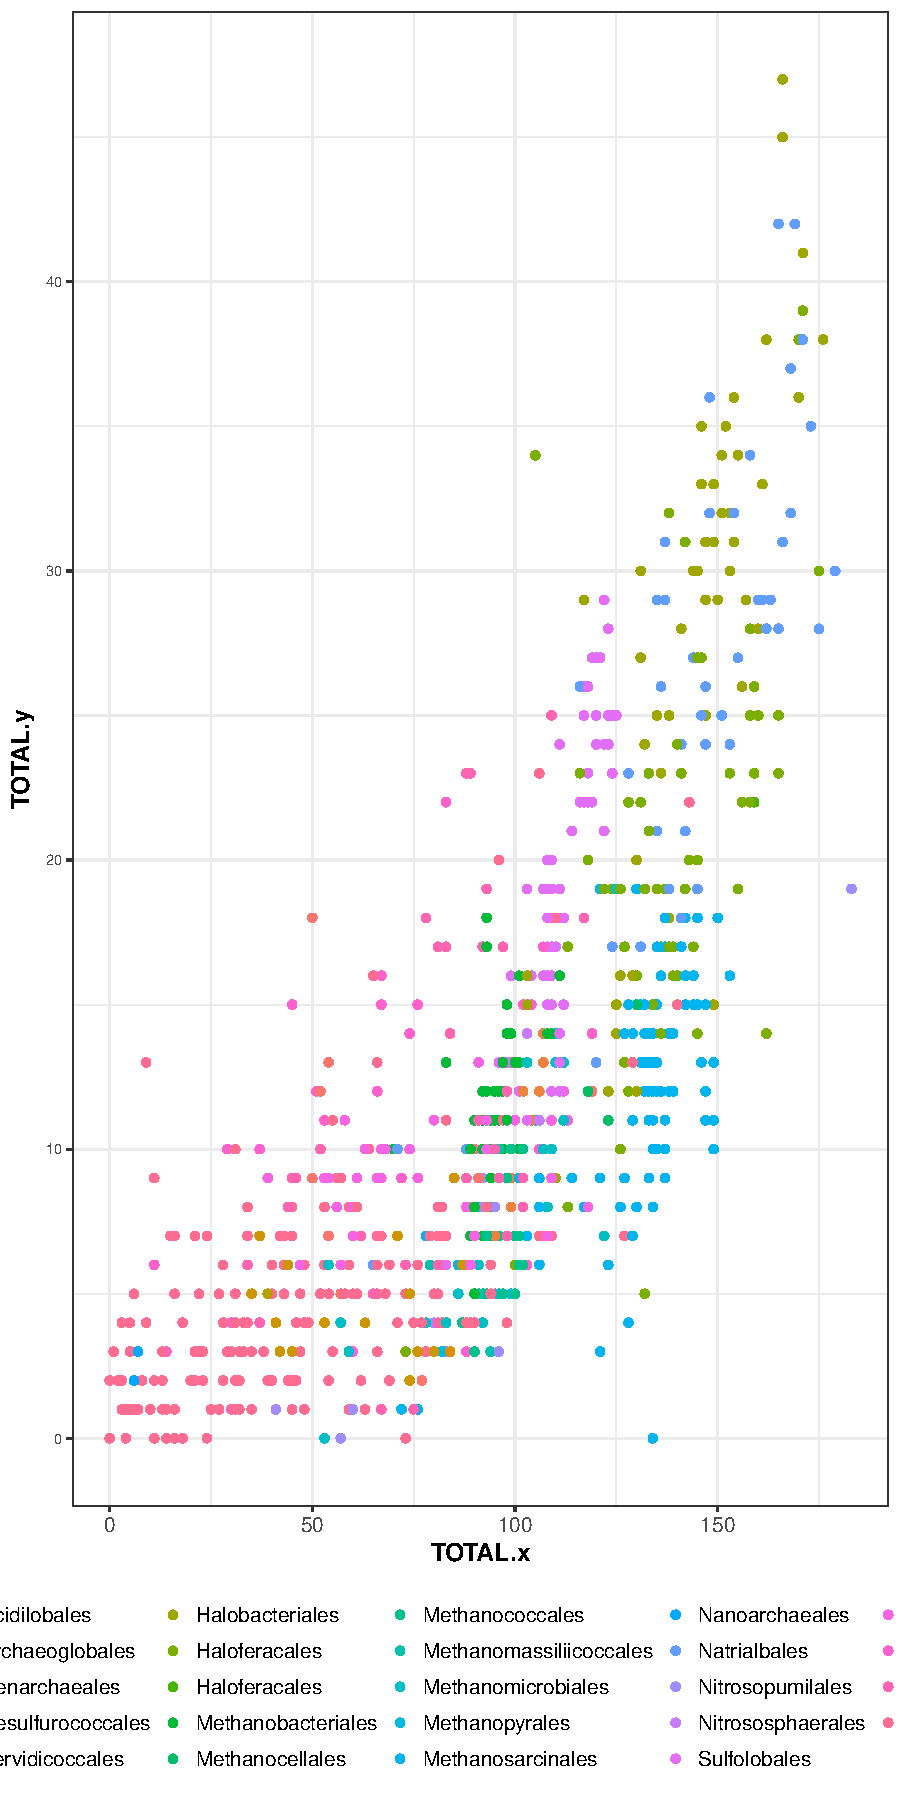
\includegraphics[angle = 0,scale = 0.5]{chapter3/ArchaeasSMASHvsExpansionsbyOrder.pdf}
  \caption[Correlation between Archaeas central pathway expansions and antismash Natural products detection]{\normalsize{Correlation between Archaeas central pathway expansions and antismash Natural products detection}}
  \label{fig:ArchaeasSMASHvsExpansionsbyOrder}
  \end{figure}
  
  Here is a reference to the expansions vs antismash NP's clusters plot:
  \autoref{fig:ArchaeasSMASHvsExpansionsbyOrder}. \clearpage 
  
  Total central pathway expansions by genome vs Total antismash cluster
  detected splitted by order
  
  \begin{figure}[h!tbp]
  \centering
  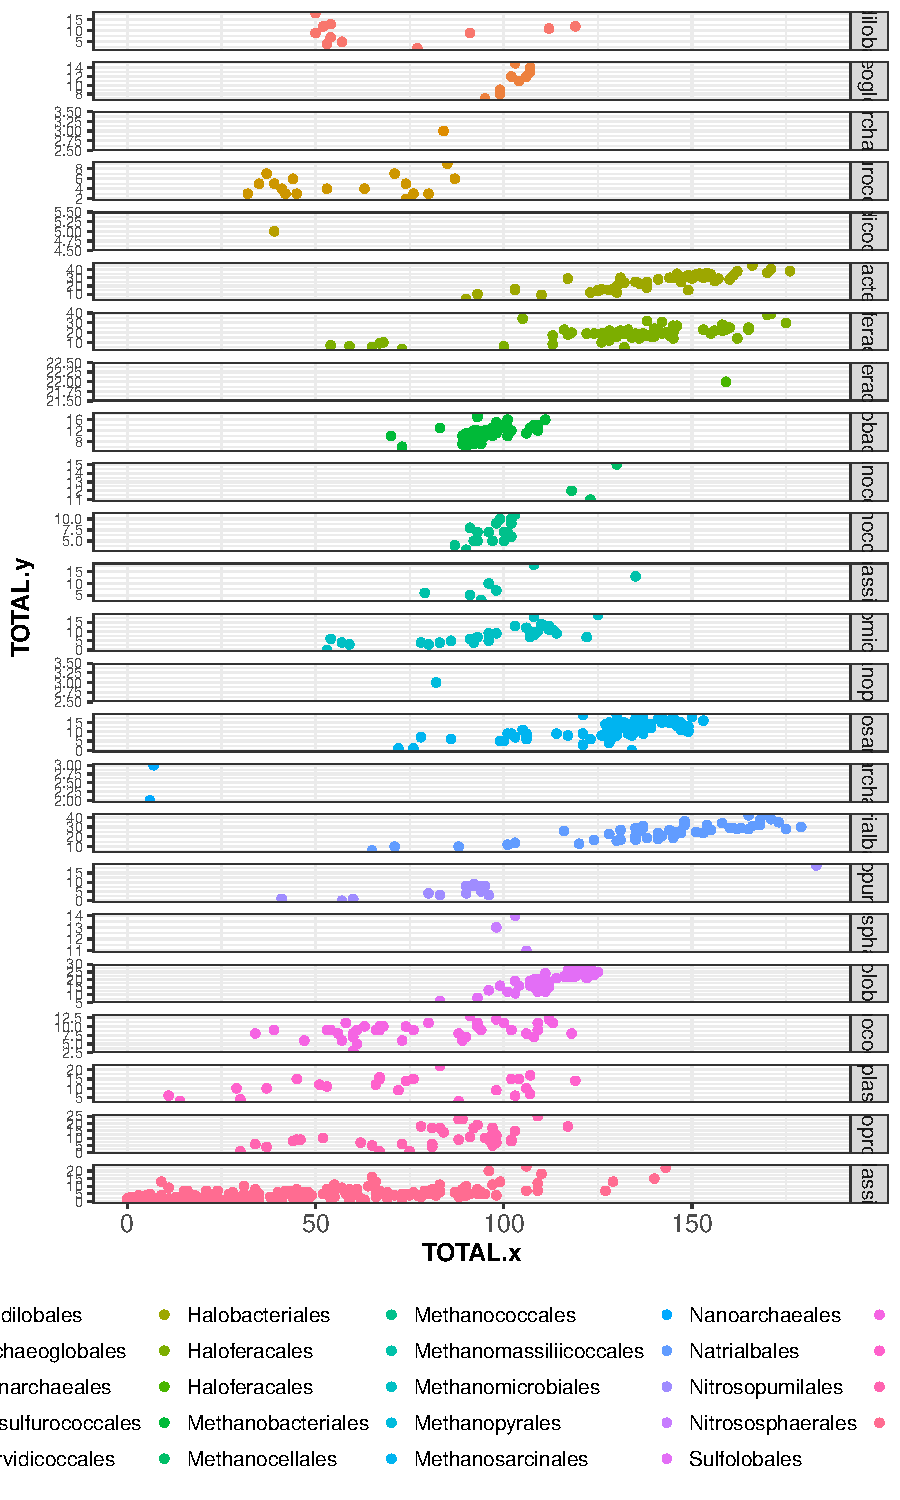
\includegraphics[angle = 0,scale = 0.5]{chapter3/ArchaeasSMASHvsExpansionsbyOrderGRID.pdf}
  \caption[Correlation between Archaeas central pathway expnasions and antismash Natural products detection]{\normalsize{Correlation between Archaeas central pathway expnasions and antismash Natural products detection}}
  \label{fig:ArchaeasSMASHvsExpansionsbyOrderGRID}
  \end{figure}
  
  Here is a reference to the expansions vs antismash NP's clusters
  splitted by order plot
  \autoref{fig:ArchaeasSMASHvsExpansionsbyOrderGRID}. \clearpage 
  
  AntisMAsh vs Expansions by taxonomic Family
  
  Natural products colured by family
  
  \begin{figure}[h!tbp]
  \centering
  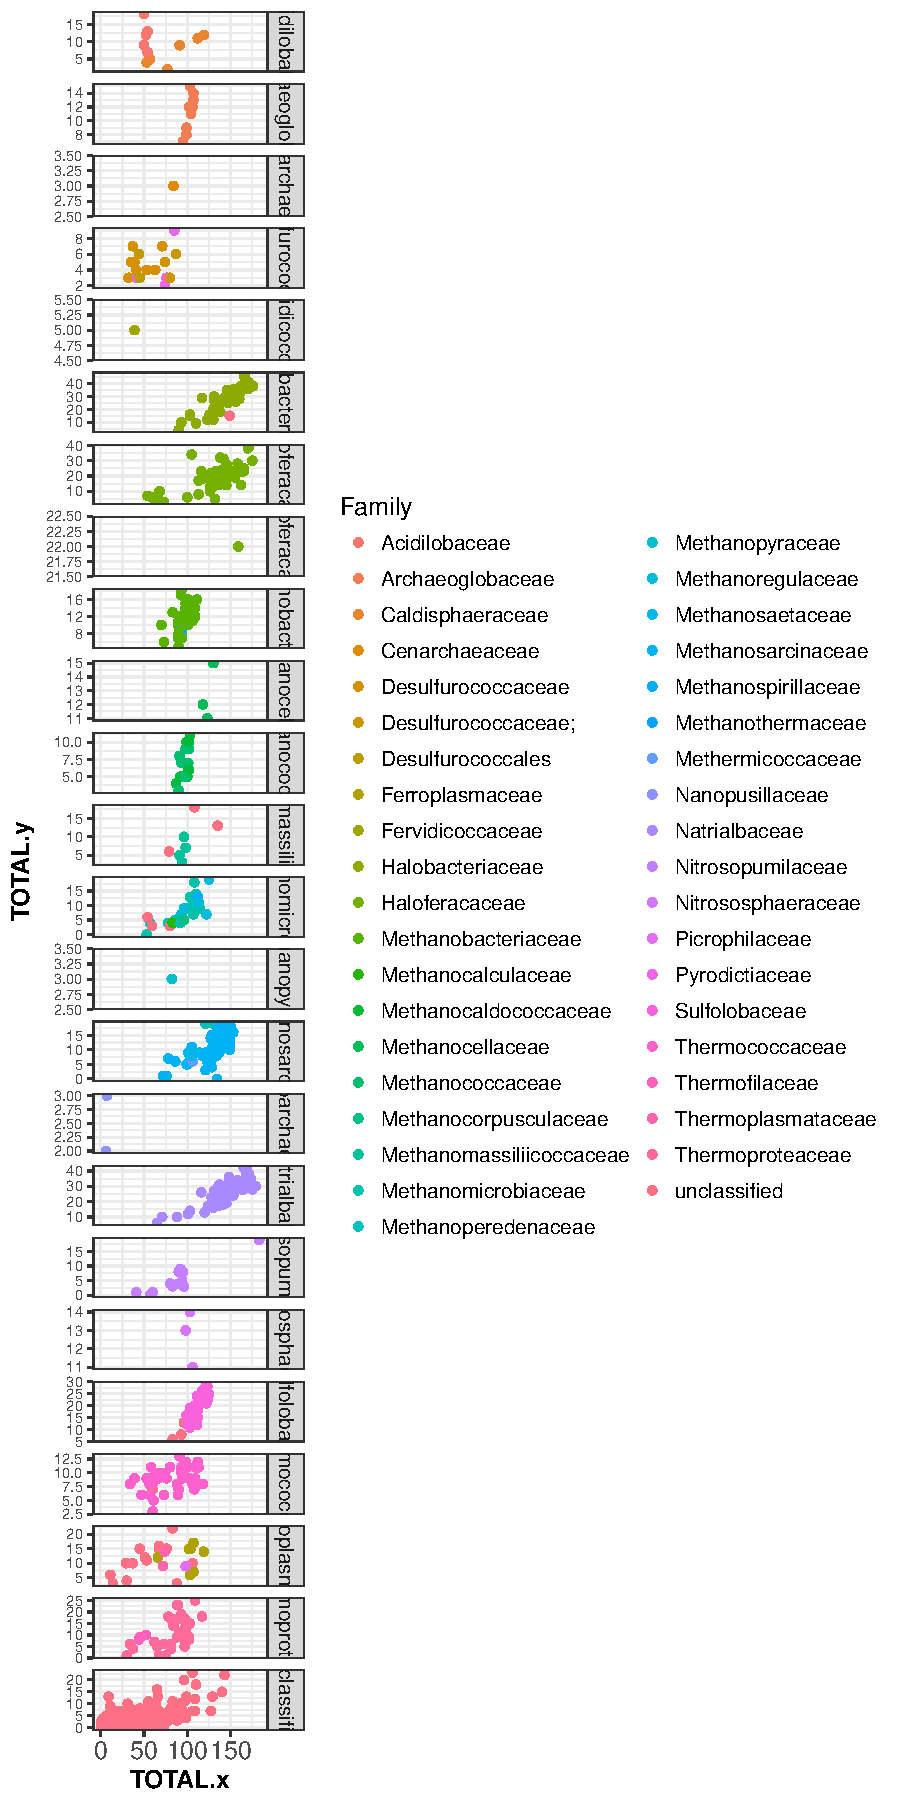
\includegraphics[angle = 0,scale = 0.6]{chapter3/Archaeasnpf.pdf}
  \caption[Archaeas Natural products by family]{\normalsize{Archaeas Natural products by family}}
  \label{fig:Archaeasnpf}
  \end{figure}
  
  Here is a reference to the Natural products colured by family plot
  \autoref{fig:Archaeasnpf}. \clearpage 
  
  \section{Selected trees from
  EvoMining}\label{selected-trees-from-evomining}
  
  Phosphoribosyl\_isomerase\_3 family\\
  Figure from EvoMining
  
  \begin{figure}[h!tbp]
  \centering
  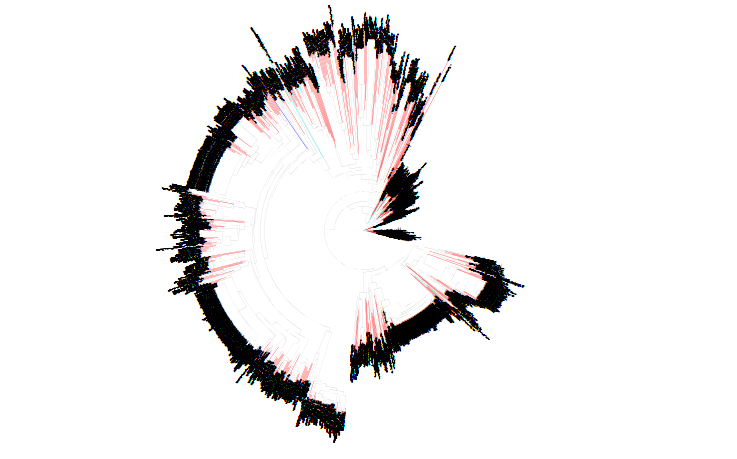
\includegraphics[angle = 180,scale = 0.25]{chapter3/tree41.png}
  \caption[Phosphoribosyl isomerase A EvoMiningtree]{\normalsize{Phosphoribosyl isomerase A EvoMiningtree}}
  \label{fig:Phosphoribosyl_isomerase_A_evo_tree}
  \end{figure}\begin{figure}[h!tbp]
  \centering
  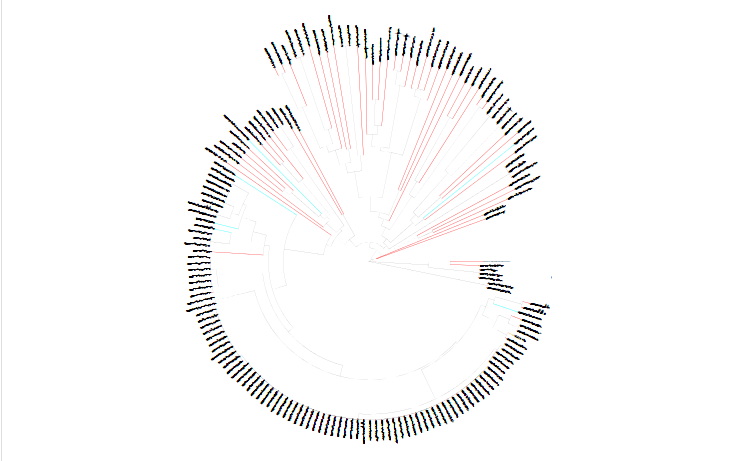
\includegraphics[angle = 180,scale = 0.25]{chapter3/tree42.png}
  \caption[Phosphoribosyl isomerase other EvoMiningtree]{\normalsize{Phosphoribosyl isomerase other EvoMiningtree}}
  \label{fig:Phosphoribosyl_isomerase_other_evo_tree}
  \end{figure}\begin{figure}[h!tbp]
  \centering
  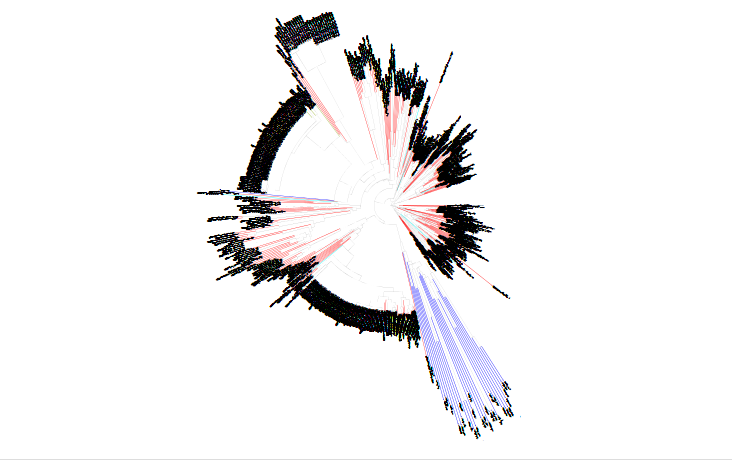
\includegraphics[angle = 180,scale = 0.25]{chapter3/tree65.png}
  \caption[Phosphoribosyl anthranilate isomerase EvoMiningtree]{\normalsize{Phosphoribosyl anthranilate isomerase EvoMiningtree}}
  \label{fig:Phosphoribosylanthranilate_isomerase_evo_tree}
  \end{figure}
  
  \clearpage 
  
  \hypertarget{section}{\section{}\label{section}}
  
  Other possible databases Archaeal signatures \emph{set of
  protein-encoding genes that function uniquely within the Archaea; most
  signature proteins have no recognizable bacterial or eukaryal homologs}
  {[}\protect\hyperlink{ref-grahamux5farchaealux5f2000}{117}{]} \#\#
  Footnotes and Endnotes
  
  You might want to footnote something.\footnote{footnote text} The
  footnote will be in a smaller font and placed appropriately. Endnotes
  work in much the same way. More information can be found about both on
  the CUS site or feel free to reach out to
  \href{mailto:data@reed.edu}{\nolinkurl{data@reed.edu}}.
  
  \section{Bibliographies}\label{bibliographies}
  
  Of course you will need to cite things, and you will probably accumulate
  an armful of sources. There are a variety of tools available for
  creating a bibliography database (stored with the .bib extension). In
  addition to BibTeX suggested below, you may want to consider using the
  free and easy-to-use tool called Zotero. The Reed librarians have
  created Zotero documentation at
  \url{http://libguides.reed.edu/citation/zotero}. In addition, a tutorial
  is available from Middlebury College at
  \url{http://sites.middlebury.edu/zoteromiddlebury/}.
  
  \emph{R Markdown} uses \emph{pandoc} (\url{http://pandoc.org/}) to build
  its bibliographies. One nice caveat of this is that you won't have to do
  a second compile to load in references as standard \LaTeX~requires. To
  cite references in your thesis (after creating your bibliography
  database), place the reference name inside square brackets and precede
  it by the ``at'' symbol. For example, here's a reference to a book about
  worrying: {[}\protect\hyperlink{ref-Molina1994}{140}{]}. This
  \texttt{Molina1994} entry appears in a file called \texttt{thesis.bib}
  in the \texttt{bib} folder. This bibliography database file was created
  by a program called BibTeX. You can call this file something else if you
  like (look at the YAML header in the main .Rmd file) and, by default, is
  to placed in the \texttt{bib} folder.
  
  For more information about BibTeX and bibliographies, see our CUS site
  (\url{http://web.reed.edu/cis/help/latex/index.html})\footnote{{[}\protect\hyperlink{ref-reedweb2007}{141}{]}}.
  There are three pages on this topic: \emph{bibtex} (which talks about
  using BibTeX, at \url{http://web.reed.edu/cis/help/latex/bibtex.html}),
  \emph{bibtexstyles} (about how to find and use the bibliography style
  that best suits your needs, at
  \url{http://web.reed.edu/cis/help/latex/bibtexstyles.html}) and
  \emph{bibman} (which covers how to make and maintain a bibliography by
  hand, without BibTeX, at
  \url{http://web.reed.edu/cis/help/latex/bibman.html}). The last page
  will not be useful unless you have only a few sources.
  
  If you look at the YAML header at the top of the main .Rmd file you can
  see that we can specify the style of the bibliography by referencing the
  appropriate csl file. You can download a variety of different style
  files at \url{https://www.zotero.org/styles}. Make sure to download the
  file into the csl folder.
  
  \paragraph{Tips for Bibliographies}\label{tips-for-bibliographies}
  
  \begin{itemize}
  \tightlist
  \item
    Like with thesis formatting, the sooner you start compiling your
    bibliography for something as large as thesis, the better. Typing in
    source after source is mind-numbing enough; do you really want to do
    it for hours on end in late April? Think of it as procrastination.
  \item
    The cite key (a citation's label) needs to be unique from the other
    entries.
  \item
    When you have more than one author or editor, you need to separate
    each author's name by the word ``and'' e.g.
    \texttt{Author\ =\ \{Noble,\ Sam\ and\ Youngberg,\ Jessica\},}.
  \item
    Bibliographies made using BibTeX (whether manually or using a manager)
    accept \LaTeX~markup, so you can italicize and add symbols as
    necessary.
  \item
    To force capitalization in an article title or where all lowercase is
    generally used, bracket the capital letter in curly braces.
  \item
    You can add a Reed Thesis citation\footnote{{[}\protect\hyperlink{ref-noble2002}{142}{]}}
    option. The best way to do this is to use the phdthesis type of
    citation, and use the optional ``type'' field to enter ``Reed thesis''
    or ``Undergraduate thesis.''
  \end{itemize}
  
  \section{Anything else?}\label{anything-else}
  
  If you'd like to see examples of other things in this template, please
  contact the Data @ Reed team (email
  \href{mailto:data@reed.edu}{\nolinkurl{data@reed.edu}}) with your
  suggestions. We love to see people using \emph{R Markdown} for their
  theses, and are happy to help.
  
  \hypertarget{refux5flabels}{\chapter{Actinobacteria EvoMining
  Results}\label{refux5flabels}}
  
  Actinobacteria is an ancient phylum \{Referencia de luis\}
  
  \section{Tables}\label{tables-1}
  
  \begin{longtable}[c]{@{}ccl@{}}
  \caption{Correlation of Inheritance Factors for Parents and Child
  \label{tab:inher}}\tabularnewline
  \toprule
  \begin{minipage}[b]{0.29\columnwidth}\centering\strut
  Factors
  \strut\end{minipage} &
  \begin{minipage}[b]{0.47\columnwidth}\centering\strut
  Correlation between Parents \& Child
  \strut\end{minipage} &
  \begin{minipage}[b]{0.16\columnwidth}\raggedright\strut
  \strut\end{minipage}\tabularnewline
  \midrule
  \endfirsthead
  \toprule
  \begin{minipage}[b]{0.29\columnwidth}\centering\strut
  Factors
  \strut\end{minipage} &
  \begin{minipage}[b]{0.47\columnwidth}\centering\strut
  Correlation between Parents \& Child
  \strut\end{minipage} &
  \begin{minipage}[b]{0.16\columnwidth}\raggedright\strut
  \strut\end{minipage}\tabularnewline
  \midrule
  \endhead
  \begin{minipage}[t]{0.29\columnwidth}\centering\strut
  GenomeDB
  \strut\end{minipage} &
  \begin{minipage}[t]{0.47\columnwidth}\centering\strut
  1245
  \strut\end{minipage} &
  \begin{minipage}[t]{0.16\columnwidth}\raggedright\strut
  \strut\end{minipage}\tabularnewline
  \begin{minipage}[t]{0.29\columnwidth}\centering\strut
  Families
  \strut\end{minipage} &
  \begin{minipage}[t]{0.47\columnwidth}\centering\strut
  65
  \strut\end{minipage} &
  \begin{minipage}[t]{0.16\columnwidth}\raggedright\strut
  \strut\end{minipage}\tabularnewline
  \bottomrule
  \end{longtable}
  
  \clearpage
  
  \subsection{Expansions BoxPlot by metabolic
  family}\label{expansions-boxplot-by-metabolic-family-1}
  
  \begin{Shaded}
  \begin{Highlighting}[]
  \KeywordTok{label}\NormalTok{(}\DataTypeTok{path =} \StringTok{"chapter4/expansion_plotActinos.pdf"}\NormalTok{, }\DataTypeTok{caption =} \StringTok{"Expansions Boxplot"}\NormalTok{,}\DataTypeTok{label =} \StringTok{"Actino_expansion_boxplot"}\NormalTok{, }\DataTypeTok{type =} \StringTok{"figure"}\NormalTok{)}
  \end{Highlighting}
  \end{Shaded}
  
  \begin{figure}[h!tbp]
  \centering
  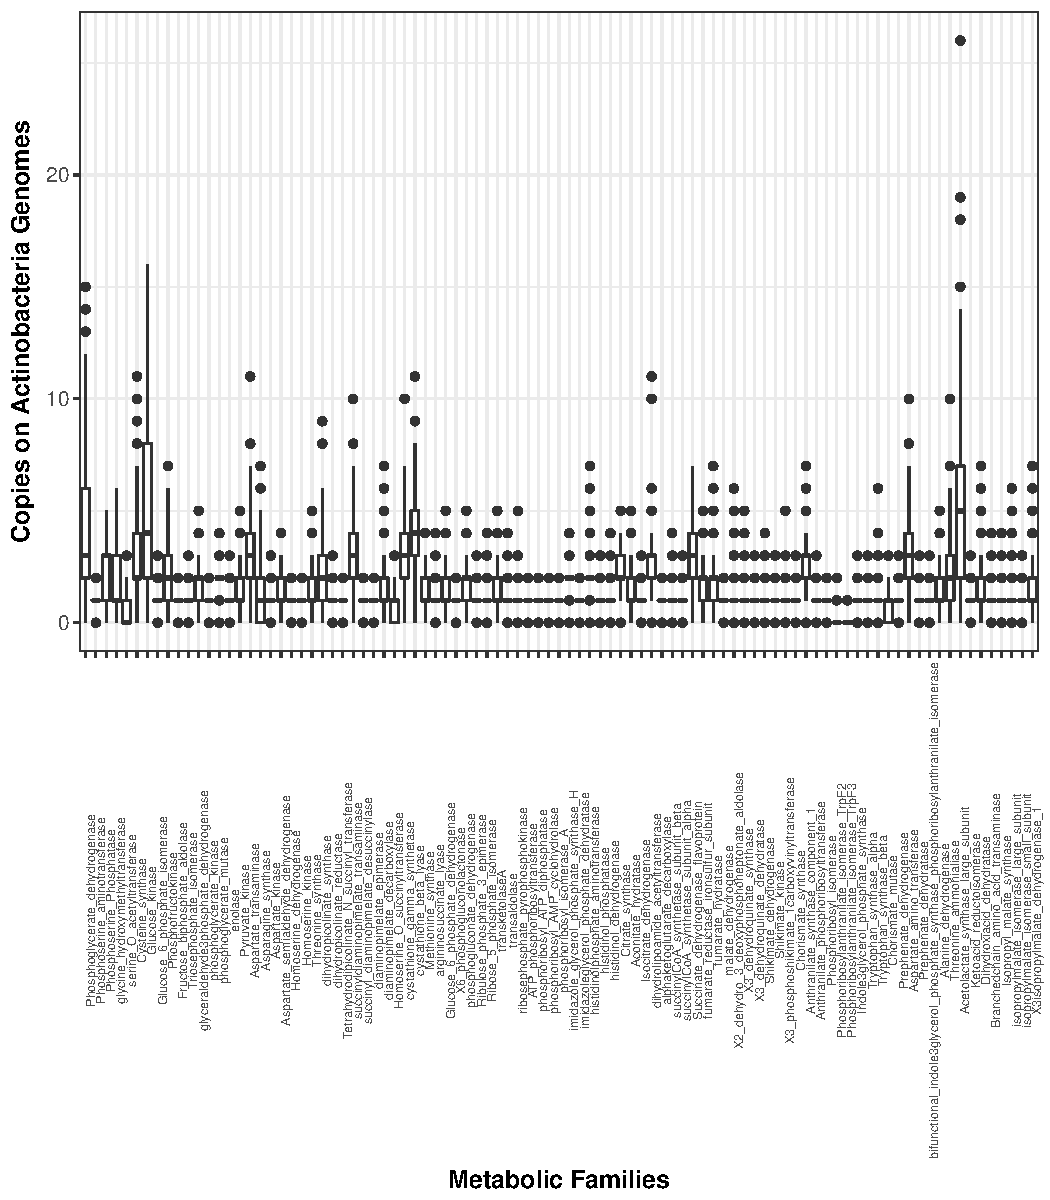
\includegraphics[angle = 0,scale = 1]{chapter4/expansion_plotActinos.pdf}
  \caption[Expansions Boxplot]{\normalsize{Expansions Boxplot}}
  \label{fig:Actino_expansion_boxplot}
  \end{figure}
  
  Here is a reference to the expansion boxplot:
  \autoref{fig:Actino_expansion_boxplot}.\\
  \clearpage 
  
  \section{Central pathway expansions}\label{central-pathway-expansions-1}
  
  Heat plot of central pathways expansions, Needs to be phylogenetically
  sorted.
  
  \begin{figure}[h!tbp]
  \centering
  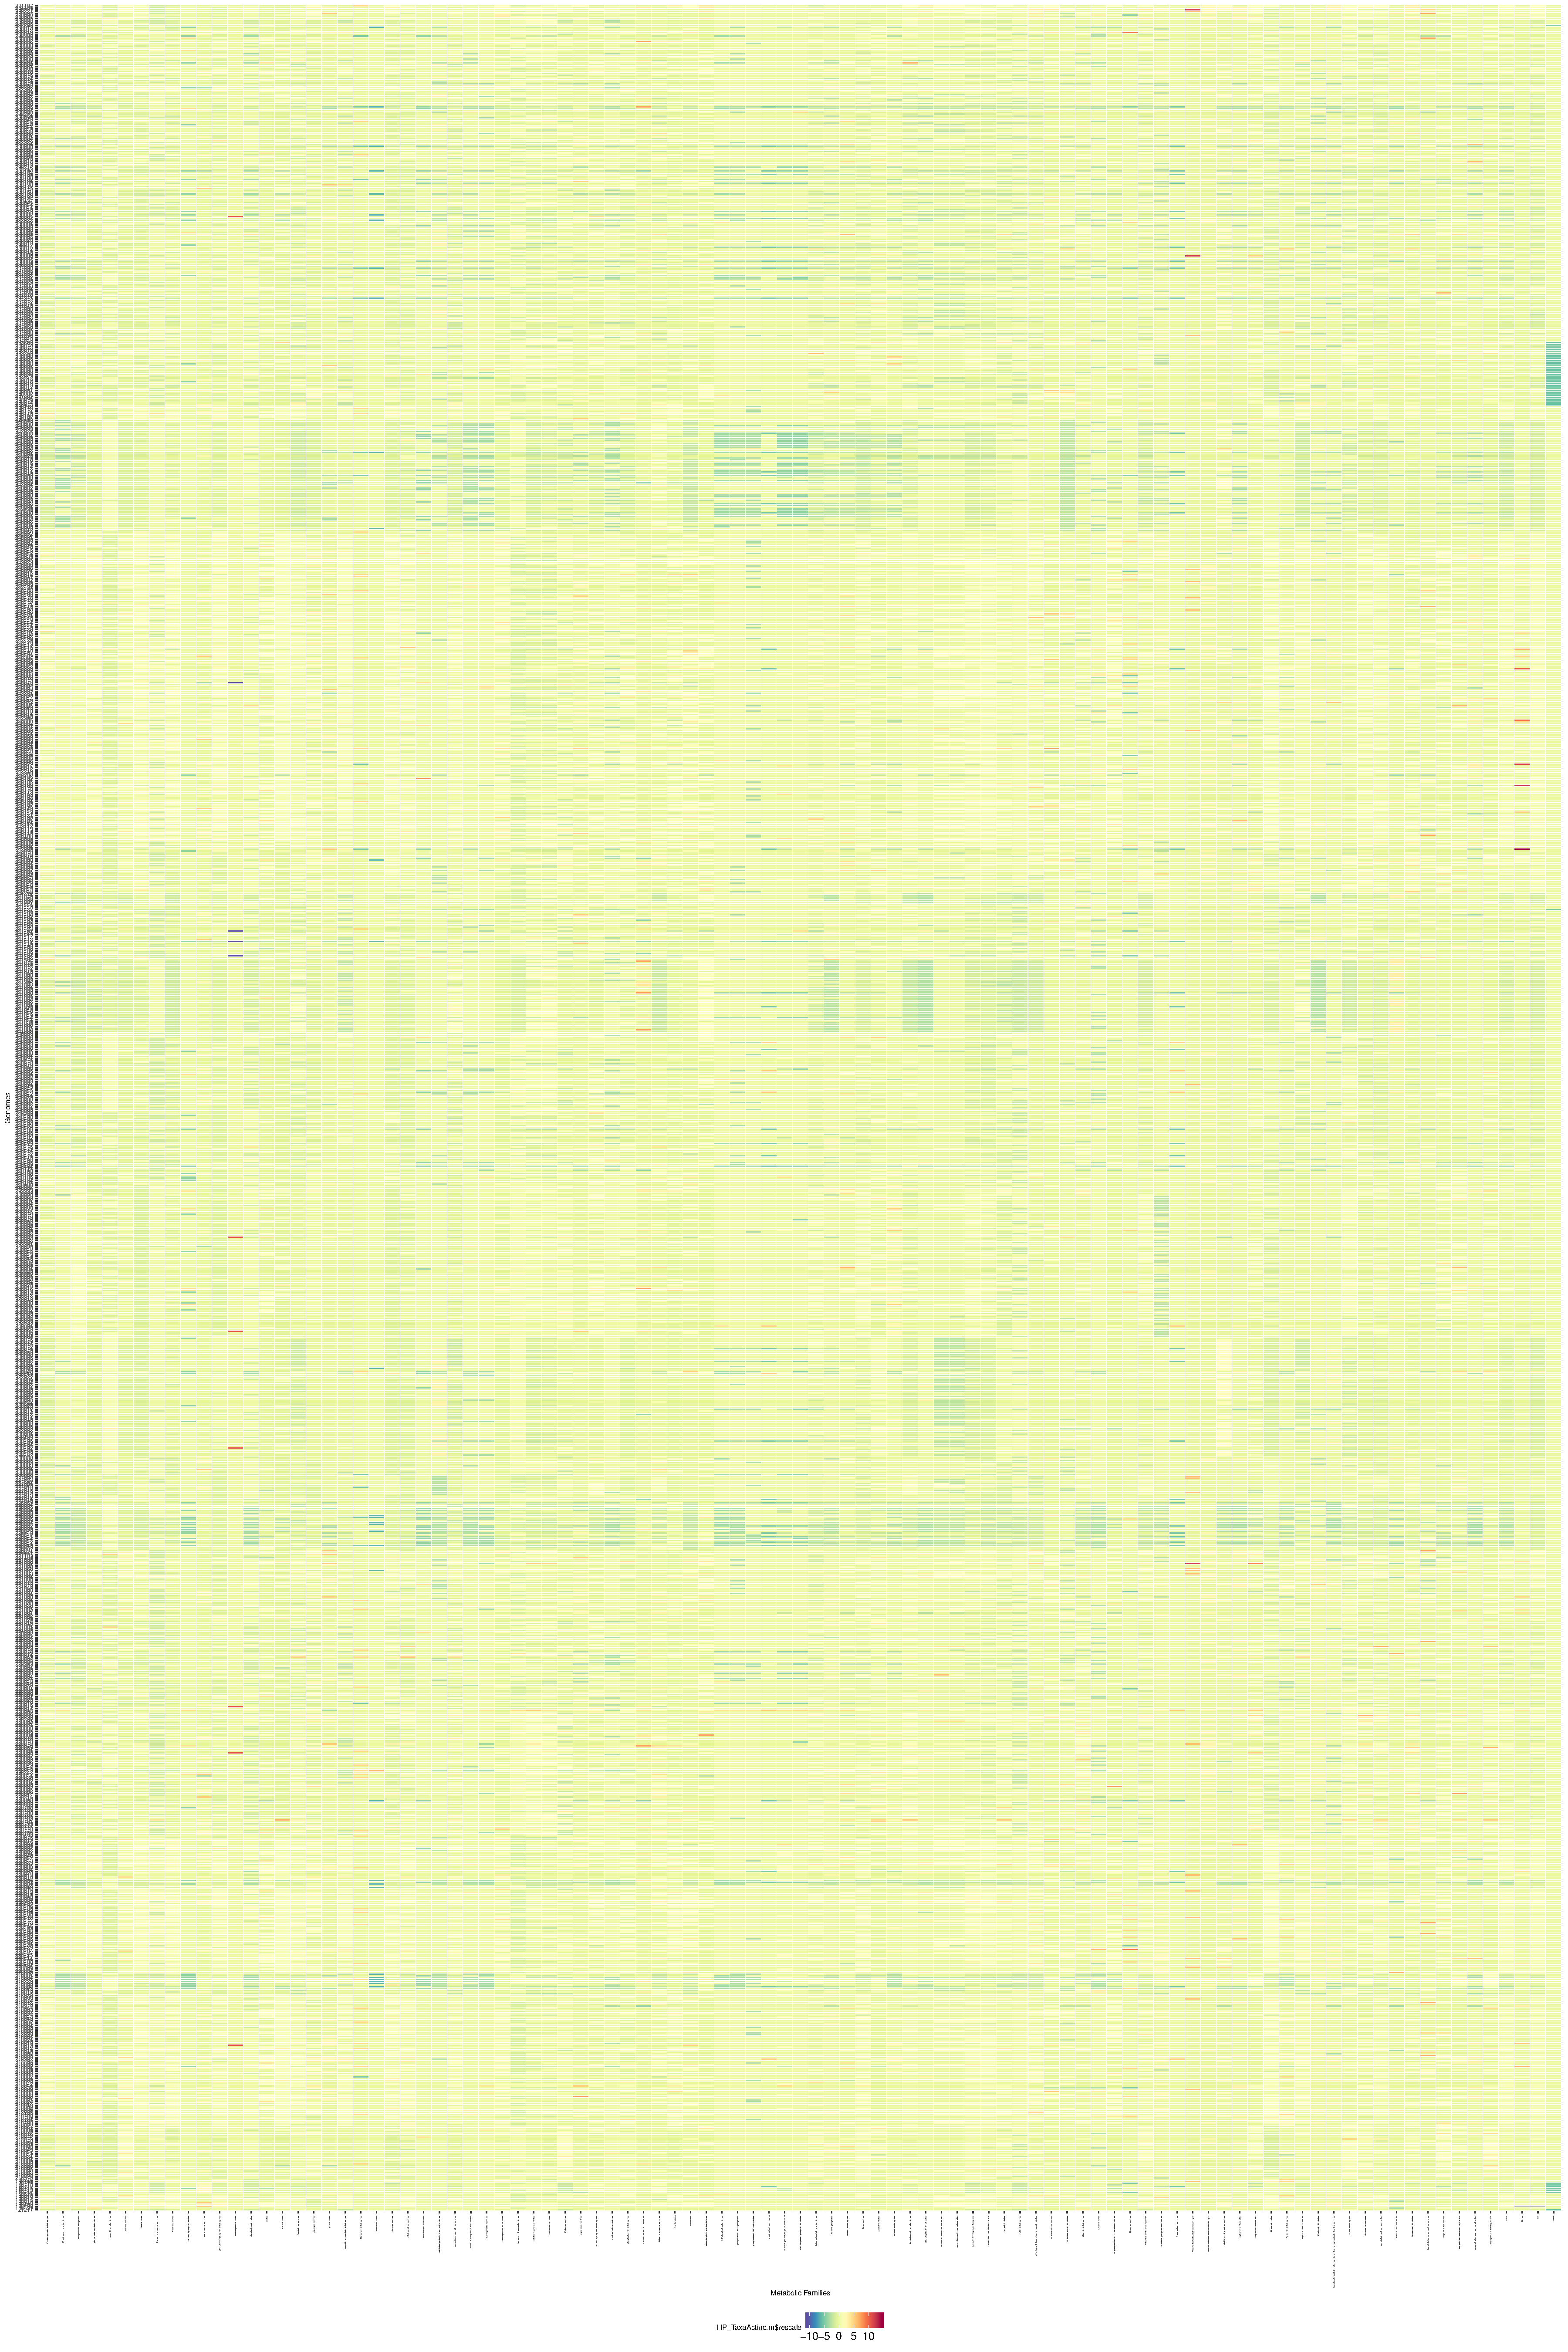
\includegraphics[angle = 0,scale = 0.7]{chapter4/HeatPlotActinos.pdf}
  \caption[Actinobacterial Heatplot]{\normalsize{Actinobacterial Heatplot}}
  \label{fig:ActinoPlot}
  \end{figure}
  
  Here is a reference to the HeatPlot: \autoref{fig:ActinoPlot}.
  \clearpage 
  
  PPP pahtway expansions restricted to \emph{Streptomycetaceae} family
  HeatPlot: \autoref{fig:ActinoPlot}.
  
  \begin{figure}[h!tbp]
  \centering
  
\includegraphics[angle = 0,scale = 0.7]{chapter4/HeatPlotStreptoPGA.pdf}
  \caption[Streptomyces Genomes expansions on PGA Aminoacids HeatPlot]{\normalsize{Streptomyces Genomes expansions on PGA Aminoacids HeatPlot}}
  \label{fig:StreptoPGAPlot}
  \end{figure}
  
  Here is a reference to the HeatPlot: \autoref{fig:StreptoPGAPlot}.
  \clearpage 
  
  \section{Genome Size correlations}\label{genome-size-correlations-1}
  
  \subsection{Correlation between genome size and AntiSMASH
  products}\label{correlation-between-genome-size-and-antismash-products-1}
  
  \begin{verbatim}
  Warning: Removed 1 rows containing missing values (geom_point).
  
  Warning: Removed 1 rows containing missing values (geom_point).
  \end{verbatim}
  
  Genome size vs Total antismash cluster coloured by order
  
  \begin{figure}[h!tbp]
  \centering
  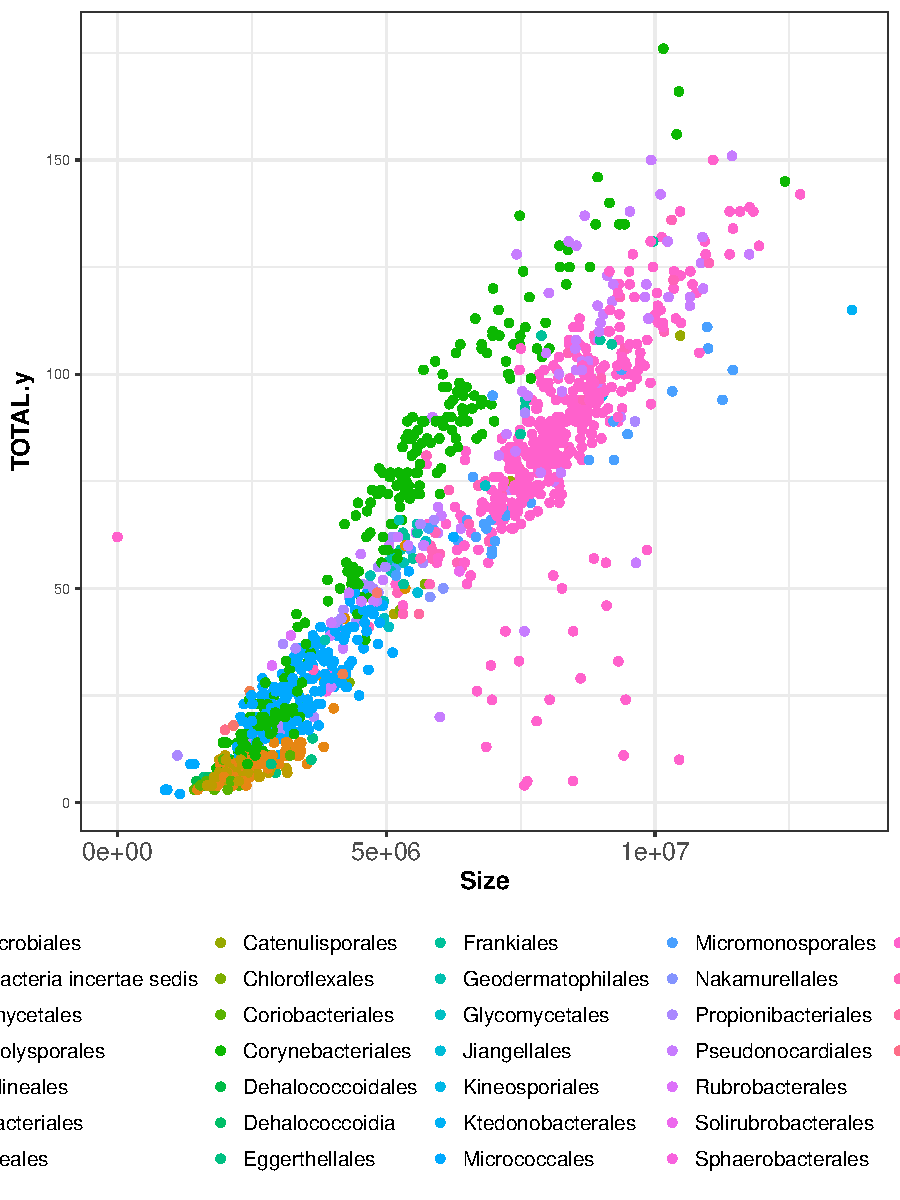
\includegraphics[angle = 0,scale = 0.6]{chapter4/ActinosSMASHvsSizebyOrder.pdf}
  \caption[Correlation between Actinos genome size and antismash Natural products detection colored by Order]{\normalsize{Correlation between Actinos genome size and antismash Natural products detection colored by Order}}
  \label{fig:ActinosSMASHvsSizebyOrder}
  \end{figure}
  
  Here is a reference to Genome size vs Total antismash cluster:
  \autoref{fig:ActinosSMASHvsSizebyOrder}. \clearpage
  
  Genome size vs Total antismash cluster detected splitted by order
  
  \begin{figure}[h!tbp]
  \centering
  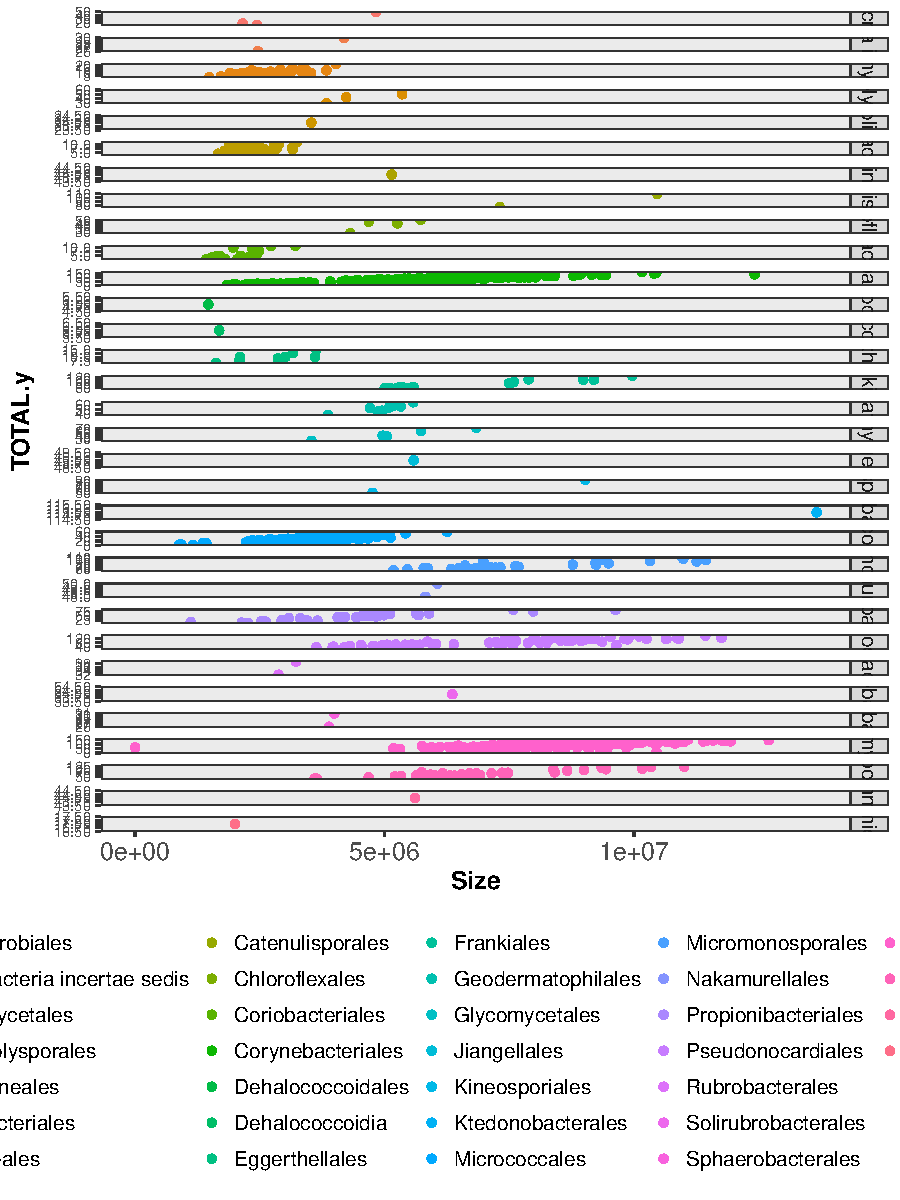
\includegraphics[angle = 0,scale = 0.6]{chapter4/ActinosSMASHvsSizeGridOrder.pdf}
  \caption[Correlation between Actinos genome size and antismash Natural products detection grided by Order]{\normalsize{Correlation between Actinos genome size and antismash Natural products detection grided by Order}}
  \label{fig:ActinosSMASHvsSizeGridOrder}
  \end{figure}
  
  Here is a reference to Correlation between genome size and antismash
  Natural products detection grided by Order plot:
  \autoref{fig:ActinosSMASHvsSizeGridOrder}. \clearpage 
  
  \subsection{Correlation between genome size and Central pathway
  expansions}\label{correlation-between-genome-size-and-central-pathway-expansions-1}
  
  \begin{verbatim}
  Warning: Removed 1 rows containing missing values (geom_point).
  
  Warning: Removed 1 rows containing missing values (geom_point).
  \end{verbatim}
  
  Genome size vs Total central pathway expansion coloured by order
  
  \begin{figure}[h!tbp]
  \centering
  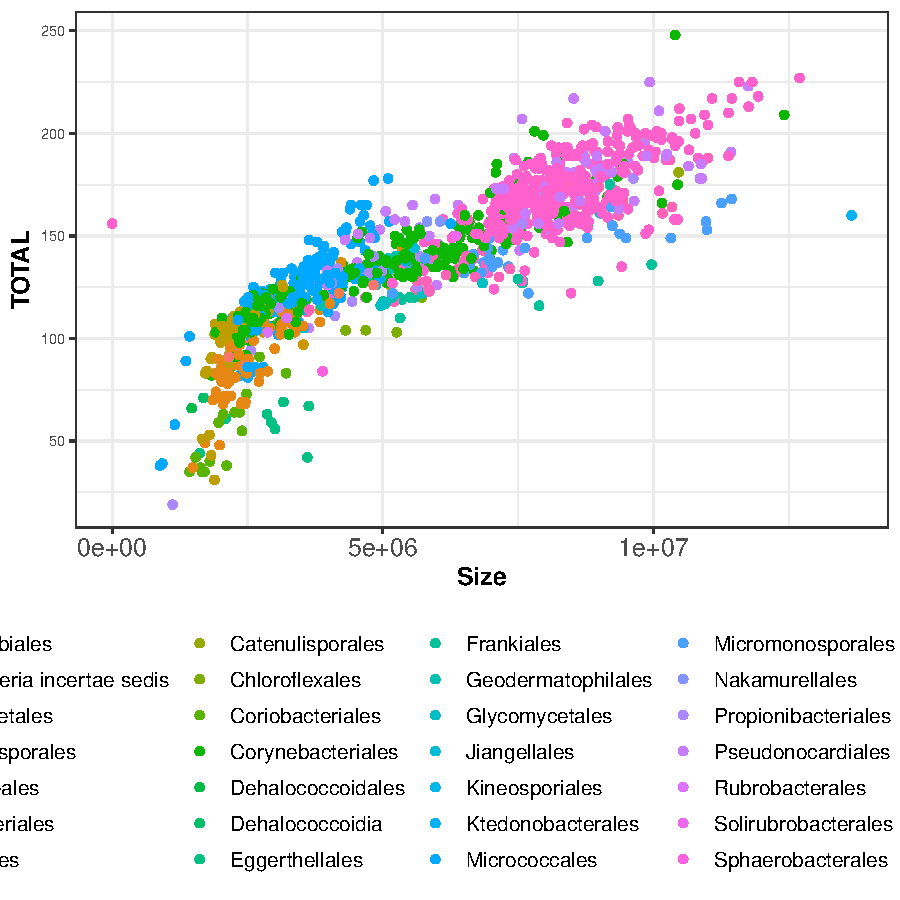
\includegraphics[angle = 0,scale = 1]{chapter4/ActinosSizevsExpansionsbyOrder.pdf}
  \caption[Correlation between Actinos genome size and central pathway expansions ]{\normalsize{Correlation between Actinos genome size and central pathway expansions }}
  \label{fig:ActinosSizevsExpansionsbyOrder}
  \end{figure}
  
  Here is a reference to the size vs Total central pathway expansion plot:
  \autoref{fig:ActinosSizevsExpansionsbyOrder}. \clearpage 
  
  Genome size vs Total central pathway expansion grided by order
  
  \begin{figure}[h!tbp]
  \centering
  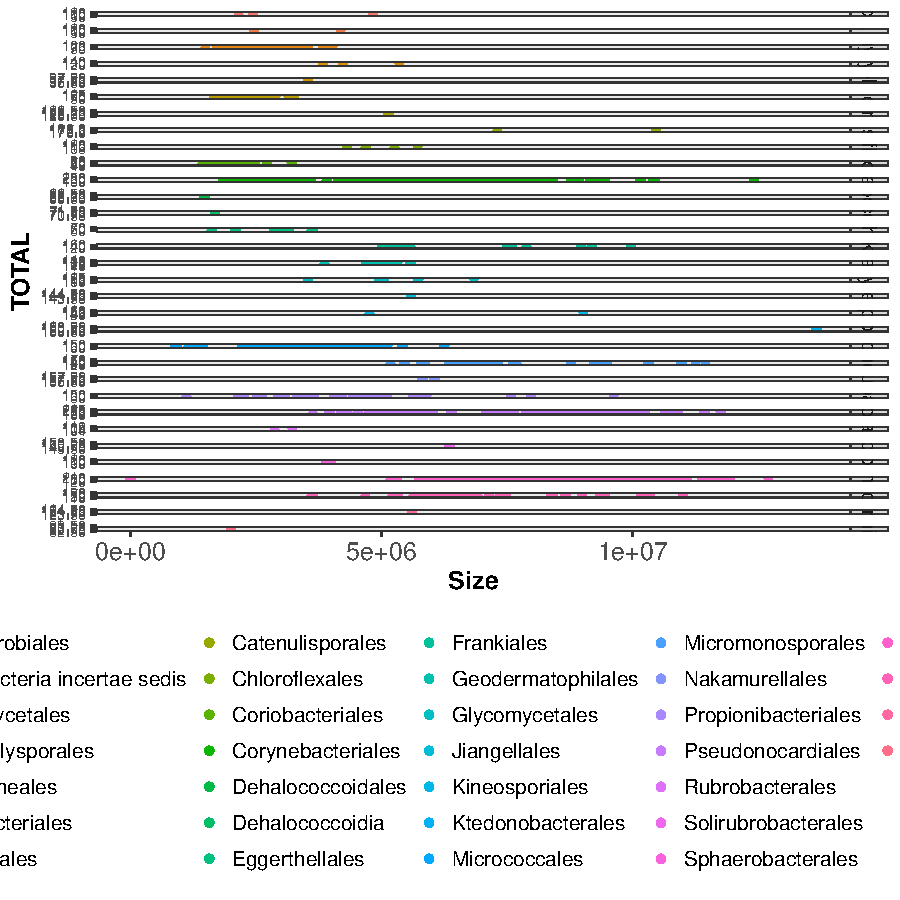
\includegraphics[angle = 0,scale = 1]{chapter4/ActinosSizevsExpansionsGridbyOrder.pdf}
  \caption[Correlation between Actinos genome size and central pathway expansions grided by order]{\normalsize{Correlation between Actinos genome size and central pathway expansions grided by order}}
  \label{fig:ActinosSizevsExpansionsGridbyOrder}
  \end{figure}
  
  Here is a reference to the Genome size vs Total central pathway
  expansion grided by order plot:
  \autoref{fig:ActinosSizevsExpansionsGridbyOrder}. \clearpage 
  
  Correlation between genome size and each of the central pathway
  families. Data are coloured by metabolic family instead of coloured by
  taxonomical order. This treatment allows to answer how differente
  metabolic families grows when genome size grow.\\
  Also I want to add form given by taxonomical order.
  
  \begin{verbatim}
  Warning: The shape palette can deal with a maximum of 6 discrete values
  because more than 6 becomes difficult to discriminate; you have
  32. Consider specifying shapes manually if you must have them.
  \end{verbatim}
  
  \begin{verbatim}
  Warning: Removed 103306 rows containing missing values (geom_point).
  \end{verbatim}
  
  \begin{verbatim}
  Warning: Removed 94 rows containing missing values (geom_point).
  \end{verbatim}
  
  Genome size vs Total central pathway expansion coloured by metabolic
  Family
  
  \begin{figure}[h!tbp]
  \centering
  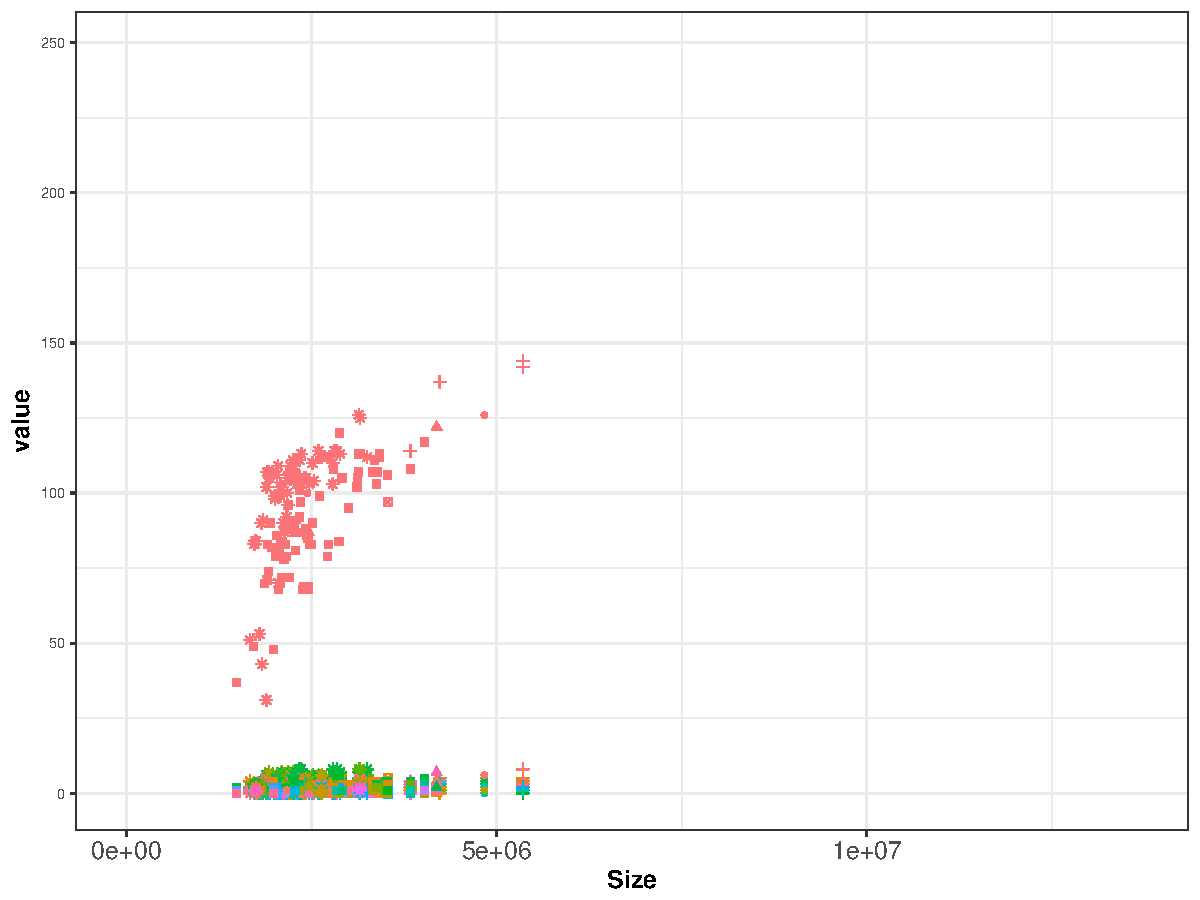
\includegraphics[angle = 0,scale = 0.6]{chapter4/ActinosSizevsExpansionsbyMetabolicFamily.pdf}
  \caption[Correlation between Actinos Genome size vs Total central pathway expansion coloured by metabolic Family]{\normalsize{Correlation between Actinos Genome size vs Total central pathway expansion coloured by metabolic Family}}
  \label{fig:ActinosSizevsExpansionsbyMetabolicFamily}
  \end{figure}
  
  Here is a reference to the Genome size vs Total central pathway
  expansion coloured by metabolic Family plot:
  \autoref{fig:ActinosSizevsExpansionsbyMetabolicFamily}. \clearpage 
  
  Future Work: Genome size vs Total central pathway expansion grided by
  metabolic Family For clarity I need to also grid and group by Metabolic
  Pathway
  
  Here is a reference to Genome size vs Total central pathway expansion
  grided by metabolic Family plot:
  \autoref{fig:ActinosExpansionsbyMetabolicFamilyGrid}. \clearpage 
  
  \section{Natural products}\label{natural-products-1}
  
  \subsection{Natural products recruitments from EvoMining
  heatplot}\label{natural-products-recruitments-from-evomining-heatplot-1}
  
  We can see natural products recruitment after central pathways
  expansions colored by their kingdom.\\
  Natural products recruited by metabolic family, colored by phylogenetic
  origin.
  
  Recruitments after central pathways expansions coloured by Kingdom
  
  \begin{figure}[h!tbp]
  \centering
  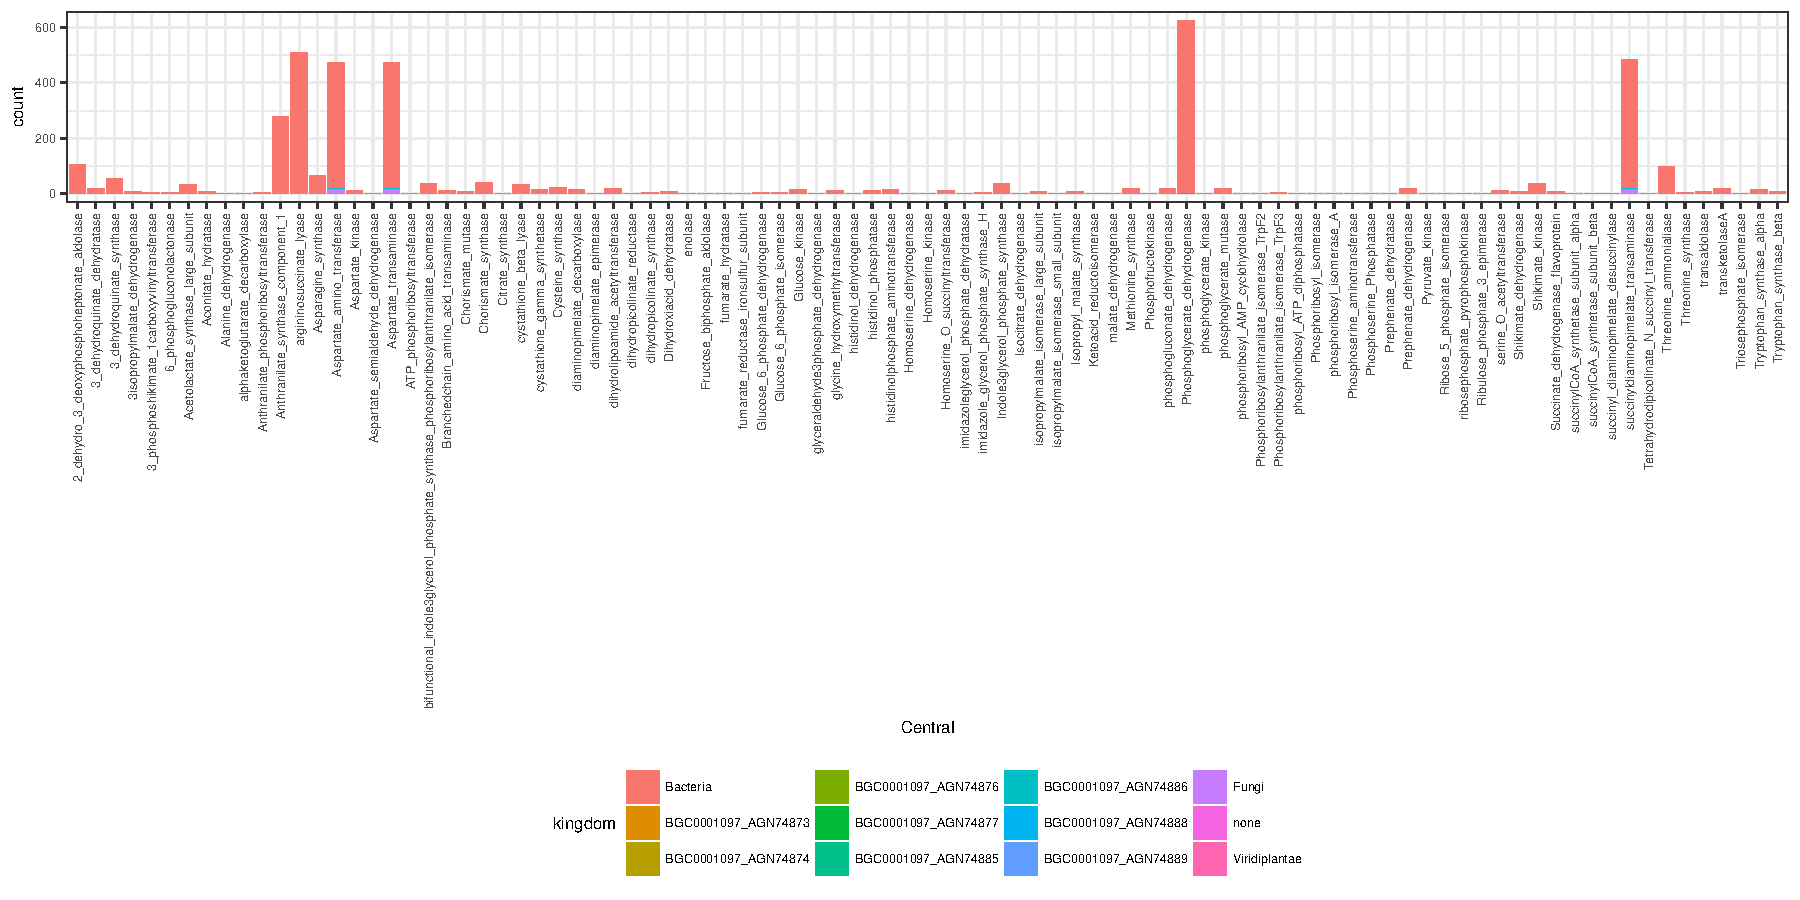
\includegraphics[angle = 0,scale = 0.6]{chapter4/ActinosRecruitmentsbyKingdom.pdf}
  \caption[Actinos Recruitmens on central families coloured by kingdom]{\normalsize{Actinos Recruitmens on central families coloured by kingdom}}
  \label{fig:ActinosRecruitmentsbyKingdom}
  \end{figure}
  
  Here is a reference to Recruitments after central pathways expansions
  colourd by Kingdom plot: \autoref{fig:ActinosRecruitmentsbyKingdom}.
  
  \clearpage 
  Recruitments after central pathways expansions colourd by taxonomy
  
  \begin{figure}[h!tbp]
  \centering
  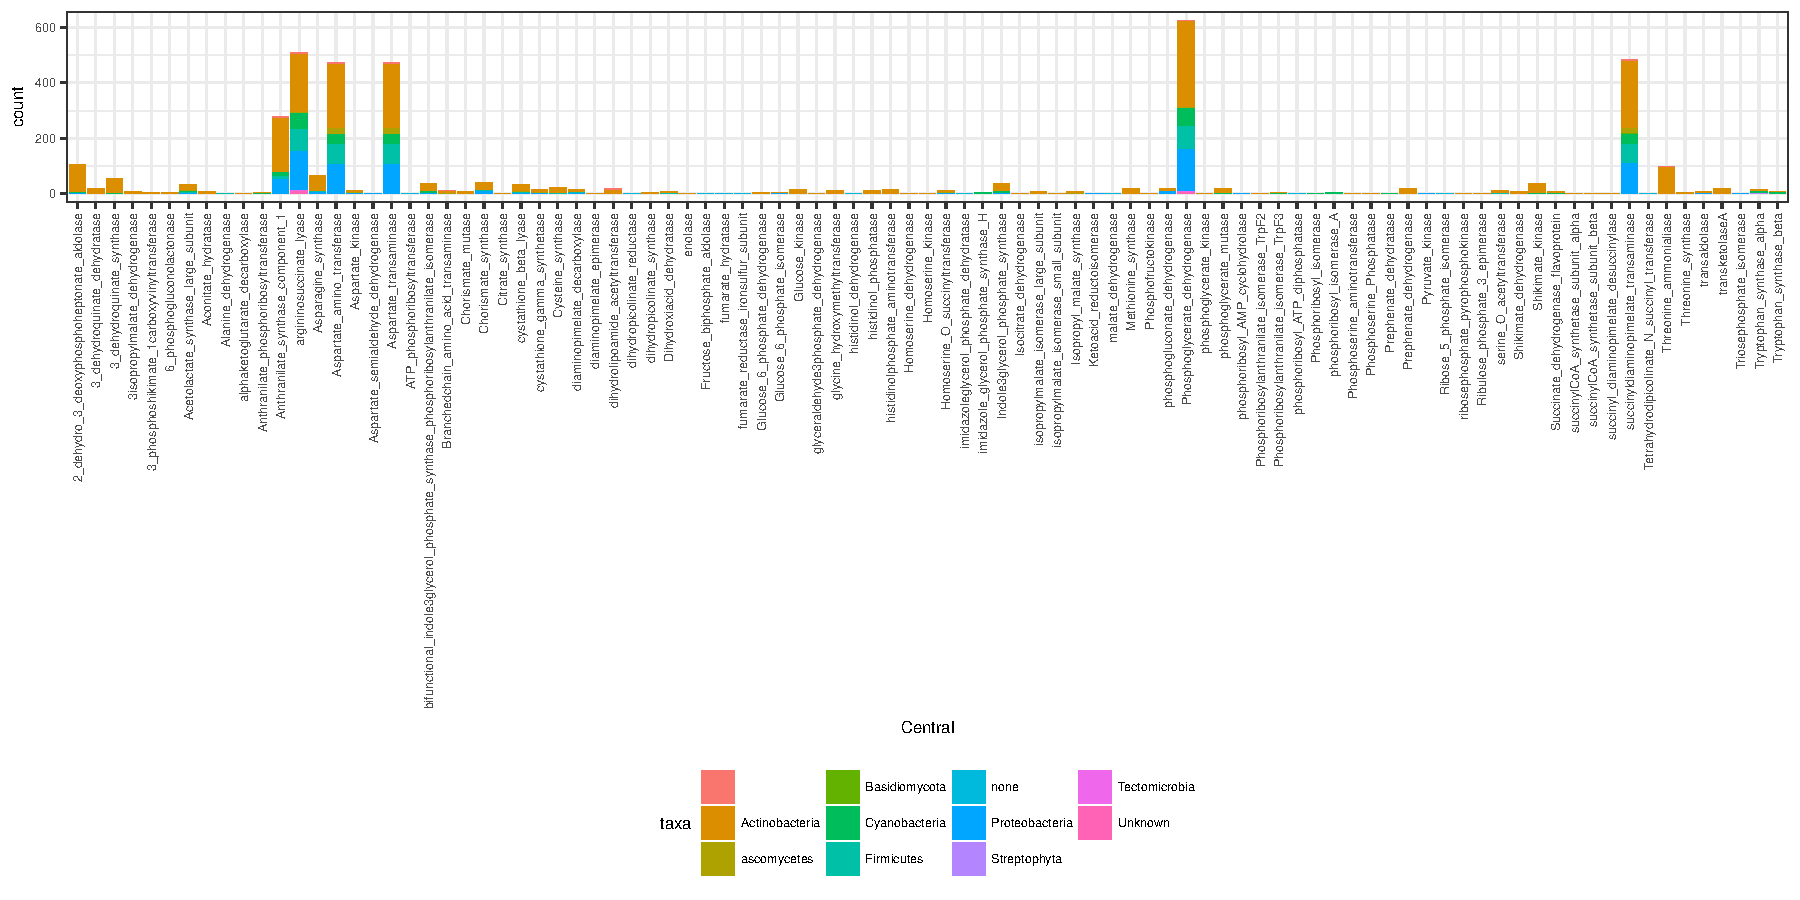
\includegraphics[angle = 0,scale = 0.5]{chapter4/ActinosRecruitmentsbyTaxa.pdf}
  \caption[Actinos Recruitmens on central families coloured by taxonomy]{\normalsize{Actinos Recruitmens on central families coloured by taxonomy}}
  \label{fig:ActinosRecruitmentsbyTaxa}
  \end{figure}
  
  Here is a reference to Recruitments after central pathways expansions
  colourd by taxa plot: \autoref{fig:ActinosRecruitmentsbyTaxa}.
  \clearpage 
  
  \section{Actinos AntiSMASH}\label{actinos-antismash}
  
  Taxonomical diversity on Actinosbacteria Data
  
  \begin{figure}[h!tbp]
  \centering
  \includegraphics[angle = 0,scale = 0.6]{chapter4/ActinosDiversity.pdf}
  \caption[Actinos Diversity]{\normalsize{Actinos Diversity}}
  \label{fig:ActinosDiversity}
  \end{figure}
  
  Here is a reference to Recruitments after central pathways expansions
  colourd by taxa plot: \autoref{fig:ActinosDiversity}. \clearpage
  
  Smash diversity
  
  \begin{figure}[h!tbp]
  \centering
  \includegraphics[angle = 0,scale = 0.5]{chapter4/ActinosSmash.pdf}
  \caption[Actinos Smash Taxonomical Diversity]{\normalsize{Actinos Smash Taxonomical Diversity}}
  \label{fig:ActinosSmash}
  \end{figure}
  
  Here is a reference to Recruitments after central pathways expansions
  colourd by taxa plot: \autoref{fig:ActinosSmash}. \clearpage
  
  \subsection{AntisSMASH vs Central
  Expansions}\label{antissmash-vs-central-expansions-1}
  
  Is it a correlation between pangenome grow and central pathways
  expansions?
  
  Total central pathway expansions by genome vs Total antismash cluster
  detected coloured by order
  
  \begin{figure}[h!tbp]
  \centering
  \includegraphics[angle = 0,scale = 0.5]{chapter4/ActinosSMASHvsExpansionsbyOrder.pdf}
  \caption[Correlation between Actinos central pathway expansions and antismash Natural products detection]{\normalsize{Correlation between Actinos central pathway expansions and antismash Natural products detection}}
  \label{fig:ActinosSMASHvsExpansionsbyOrder}
  \end{figure}
  
  Here is a reference to the expansions vs antismash NP's clusters plot:
  \autoref{fig:ActinosSMASHvsExpansionsbyOrder}. \clearpage 
  
  Total central pathway expansions by genome vs Total antismash cluster
  detected splitted by order
  
  \begin{figure}[h!tbp]
  \centering
  \includegraphics[angle = 0,scale = 0.5]{chapter4/ActinosSMASHvsExpansionsbyOrderGRID.pdf}
  \caption[Correlation between Actinos central pathway expnasions and antismash Natural products detection]{\normalsize{Correlation between Actinos central pathway expnasions and antismash Natural products detection}}
  \label{fig:ActinosSMASHvsExpansionsbyOrderGRID}
  \end{figure}
  
  Here is a reference to the expansions vs antismash NP's clusters
  splitted by order plot
  \autoref{fig:ActinosSMASHvsExpansionsbyOrderGRID}. \clearpage 
  
  AntisMAsh vs Expansions by taxonomic Family
  
  Natural products colured by family
  
  \begin{figure}[h!tbp]
  \centering
  \includegraphics[angle = 0,scale = 0.6]{chapter4/Actinosnpf.pdf}
  \caption[Actinos Natural products by family]{\normalsize{Actinos Natural products by family}}
  \label{fig:Actinosnpf}
  \end{figure}
  
  Here is a reference to the Natural products colured by family plot
  \autoref{fig:Actinosnpf}. \clearpage 
  
  \section{Selected trees from
  EvoMining}\label{selected-trees-from-evomining-1}
  
  \begin{figure}[h!tbp]
  \centering
  \includegraphics[angle = 180,scale = 0.3]{chapter4/tree15.png}
  \caption[Enolase EvoMiningtree]{\normalsize{Enolase EvoMiningtree}}
  \label{fig:enolase_evo_tree}
  \end{figure}\begin{figure}[h!tbp]
  \centering
  \includegraphics[angle = 180,scale = 0.3]{chapter4/tree73.png}
  \caption[Phosphoribosyl isomerase EvoMiningtree]{\normalsize{Phosphoribosyl isomerase EvoMiningtree}}
  \label{fig:Phosphoribosyl_isomerase_evo_tree}
  \end{figure}\begin{figure}[h!tbp]
  \centering
  \includegraphics[angle = 180,scale = 0.3]{chapter4/tree47.png}
  \caption[Phosphoribosyl isomerase A EvoMiningtree]{\normalsize{Phosphoribosyl isomerase A EvoMiningtree}}
  \label{fig:Phosphoribosyl_isomerase_A_evo_tree}
  \end{figure}\begin{figure}[h!tbp]
  \centering
  \includegraphics[angle = 180,scale = 0.3]{chapter4/tree69.png}
  \caption[phosphoshikimate carboxyvinyltransferase EvoMiningtree]{\normalsize{phosphoshikimate carboxyvinyltransferase EvoMiningtree}}
  \label{fig:phosphoshikimate_c_evo_tree}
  \end{figure}
  
  \clearpage 
  
  \hypertarget{refux5flabels}{\chapter{Cyanobacteria EvoMining
  Results}\label{refux5flabels}}
  
  Cyanobacteria phylum \{Referencia\}\\
  Cyanobacteria is a photosynthetic phylum that inhabits a broad range of
  habitats. The broad adaptive potential is on part driven by gene-family
  enlargment {[}\protect\hyperlink{ref-larssonux5fgenomeux5f2011}{128}{]}
  by the analysis of 58 Cyanobacterial genomes concludes ancestor of
  cyanobacteria had a genome size of approx. 4.5 Mbp. Cyanobacteria
  produces natural products as pigments and toxins
  {[}\protect\hyperlink{ref-whittonux5fecologyux5f2012}{129}{]} Example of
  a PriA cluster
  toxins{[}\protect\hyperlink{ref-moustafaux5foriginux5f2009}{94}{]}
  
  Fossil record situates Cyanobacteria
  {[}\protect\hyperlink{ref-whittonux5fecologyux5f2012}{129}{]} Molecular
  record and metabolic propoerties at
  {[}\protect\hyperlink{ref-battistuzziux5fgenomicux5f2004}{132}{]}
  
  \section{Tables}\label{tables-2}
  
  \begin{longtable}[c]{@{}cc@{}}
  \caption{Families on Cyanobacteria \label{tab:inher}}\tabularnewline
  \toprule
  Factors & Correlation between Parents \& Child\tabularnewline
  \midrule
  \endfirsthead
  \toprule
  Factors & Correlation between Parents \& Child\tabularnewline
  \midrule
  \endhead
  GenomeDB & 1245\tabularnewline
  Families & 65\tabularnewline
  \bottomrule
  \end{longtable}
  
  \clearpage
  
  \subsection{Expansions BoxPlot by metabolic
  family}\label{expansions-boxplot-by-metabolic-family-2}
  
  \begin{Shaded}
  \begin{Highlighting}[]
  \KeywordTok{label}\NormalTok{(}\DataTypeTok{path =} \StringTok{"chapter5/expansion_plotCyanos.pdf"}\NormalTok{, }\DataTypeTok{caption =} \StringTok{"Expansions Boxplot"}\NormalTok{,}\DataTypeTok{label =} \StringTok{"Cyano_expansion_boxplot"}\NormalTok{, }\DataTypeTok{type =} \StringTok{"figure"}\NormalTok{)}
  \end{Highlighting}
  \end{Shaded}
  
  \begin{figure}[h!tbp]
  \centering
  \includegraphics[angle = 0,scale = 1]{chapter5/expansion_plotCyanos.pdf}
  \caption[Expansions Boxplot]{\normalsize{Expansions Boxplot}}
  \label{fig:Cyano_expansion_boxplot}
  \end{figure}
  
  Here is a reference to the expansion boxplot:
  \autoref{fig:Cyano_expansion_boxplot}.\\
  \clearpage 
  
  \section{Central pathway expansions}\label{central-pathway-expansions-2}
  
  Heat plot of central pathways expansions, Needs to be phylogenetically
  sorted.
  
  \begin{figure}[h!tbp]
  \centering
  \includegraphics[angle = 0,scale = 0.6]{chapter5/HeatPlot.pdf}
  \caption[Cyanobacterial Heatplot]{\normalsize{Cyanobacterial Heatplot}}
  \label{fig:CyanoPlot}
  \end{figure}
  
  Here is a reference to the HeatPlot: \autoref{fig:CyanoPlot}.
  \clearpage 
  
  \section{Genome Size correlations}\label{genome-size-correlations-2}
  
  \subsection{Correlation between genome size and AntiSMASH
  products}\label{correlation-between-genome-size-and-antismash-products-2}
  
  Genome size vs Total antismash cluster coloured by order
  
  \begin{figure}[h!tbp]
  \centering
  \includegraphics[angle = 0,scale = 0.6]{chapter5/SMASHvsSizebyOrder.pdf}
  \caption[Correlation between genome size and antismash Natural products detection colored by Order]{\normalsize{Correlation between genome size and antismash Natural products detection colored by Order}}
  \label{fig:SMASHvsSizebyOrder}
  \end{figure}
  
  Here is a reference to Genome size vs Total antismash cluster:
  \autoref{fig:SMASHvsSizebyOrder}. \clearpage
  
  Genome size vs Total antismash cluster detected splitted by order
  
  \begin{figure}[h!tbp]
  \centering
  \includegraphics[angle = 0,scale = 0.6]{chapter5/SMASHvsSizeGridOrder.pdf}
  \caption[Correlation between genome size and antismash Natural products detection grided by Order]{\normalsize{Correlation between genome size and antismash Natural products detection grided by Order}}
  \label{fig:SMASHvsSizeGridOrder}
  \end{figure}
  
  Here is a reference to Correlation between genome size and antismash
  Natural products detection grided by Order plot:
  \autoref{fig:SMASHvsSizeGridOrder}. \clearpage 
  
  \subsection{Correlation between genome size and Central pathway
  expansions}\label{correlation-between-genome-size-and-central-pathway-expansions-2}
  
  Genome size vs Total central pathway expansion coloured by order
  
  \begin{figure}[h!tbp]
  \centering
  \includegraphics[angle = 0,scale = 1]{chapter5/SizevsExpansionsbyOrder.pdf}
  \caption[Correlation between genome size and central pathway expansions ]{\normalsize{Correlation between genome size and central pathway expansions }}
  \label{fig:SizevsExpansionsbyOrder}
  \end{figure}
  
  Here is a reference to the size vs Total central pathway expansion plot:
  \autoref{fig:SizevsExpansionsbyOrder}. \clearpage 
  
  Genome size vs Total central pathway expansion grided by order
  
  \begin{figure}[h!tbp]
  \centering
  \includegraphics[angle = 0,scale = 1]{chapter5/SizevsExpansionsGridbyOrder.pdf}
  \caption[Correlation between genome size and central pathway expansions grided by order]{\normalsize{Correlation between genome size and central pathway expansions grided by order}}
  \label{fig:SizevsExpansionsGridbyOrder}
  \end{figure}
  
  Here is a reference to the Genome size vs Total central pathway
  expansion grided by order plot:
  \autoref{fig:SizevsExpansionsGridbyOrder}. \clearpage 
  
  Correlation between genome size and each of the central pathway
  families. Data are coloured by metabolic family instead of coloured by
  taxonomical order. This treatment allows to answer how differente
  metabolic families grows when genome size grow.\\
  Also I want to add form given by taxonomical order.
  
  \begin{verbatim}
  Warning: The shape palette can deal with a maximum of 6 discrete values
  because more than 6 becomes difficult to discriminate; you have
  10. Consider specifying shapes manually if you must have them.
  \end{verbatim}
  
  \begin{verbatim}
  Warning: Removed 20418 rows containing missing values (geom_point).
  \end{verbatim}
  
  Genome size vs Total central pathway expansion coloured by metabolic
  Family
  
  \begin{figure}[h!tbp]
  \centering
  \includegraphics[angle = 0,scale = 0.6]{chapter5/SizevsExpansionsbyMetabolicFamily.pdf}
  \caption[Correlation between Genome size vs Total central pathway expansion coloured by metabolic Family]{\normalsize{Correlation between Genome size vs Total central pathway expansion coloured by metabolic Family}}
  \label{fig:SizevsExpansionsbyMetabolicFamily}
  \end{figure}
  
  Here is a reference to the Genome size vs Total central pathway
  expansion coloured by metabolic Family plot:
  \autoref{fig:SizevsExpansionsbyMetabolicFamily}. \clearpage 
  
  Future Work: Genome size vs Total central pathway expansion grided by
  metabolic Family For clarity I need to also grid and group by Metabolic
  Pathway
  
  Here is a reference to Genome size vs Total central pathway expansion
  grided by metabolic Family plot:
  \autoref{fig:ExpansionsbyMetabolicFamilyGrid}. \clearpage 
  
  \section{Natural products}\label{natural-products-2}
  
  \subsection{Natural products recruitments from EvoMining
  heatplot}\label{natural-products-recruitments-from-evomining-heatplot-2}
  
  We can see natural products recruitment after central pathways
  expansions colored by their kingdom.\\
  Natural products recruited by metabolic family, colored by phylogenetic
  origin.
  
  Recruitments after central pathways expansions coloured by Kingdom
  
  \begin{figure}[h!tbp]
  \centering
  \includegraphics[angle = 0,scale = 0.6]{chapter5/RecruitmentsbyKingdom.pdf}
  \caption[Recruitmens on central families coloured by kingdom]{\normalsize{Recruitmens on central families coloured by kingdom}}
  \label{fig:RecruitmentsbyKingdom}
  \end{figure}
  
  Here is a reference to Recruitments after central pathways expansions
  colourd by Kingdom plot: \autoref{fig:RecruitmentsbyKingdom}.
  
  \clearpage 
  Recruitments after central pathways expansions colourd by taxonomy
  
  \begin{figure}[h!tbp]
  \centering
  \includegraphics[angle = 0,scale = 0.5]{chapter5/RecruitmentsbyTaxa.pdf}
  \caption[Recruitmens on central families coloured by taxonomy]{\normalsize{Recruitmens on central families coloured by taxonomy}}
  \label{fig:RecruitmentsbyTaxa}
  \end{figure}
  
  Here is a reference to Recruitments after central pathways expansions
  colourd by taxa plot: \autoref{fig:RecruitmentsbyTaxa}. \clearpage 
  
  \section{Cyanobacterias AntiSMASH}\label{cyanobacterias-antismash}
  
  Taxonomical diversity on Cyanobacteria Data
  
  \begin{figure}[h!tbp]
  \centering
  \includegraphics[angle = 0,scale = 0.6]{chapter5/Diversity.pdf}
  \caption[Diversity]{\normalsize{Diversity}}
  \label{fig:Diversity}
  \end{figure}
  
  Here is a reference to Recruitments after central pathways expansions
  colourd by taxa plot: \autoref{fig:Diversity}. \clearpage
  
  Smash diversity
  
  \begin{figure}[h!tbp]
  \centering
  \includegraphics[angle = 0,scale = 0.5]{chapter5/Smash.pdf}
  \caption[Smash]{\normalsize{Smash}}
  \label{fig:Smash Taxonomical Diversity}
  \end{figure}
  
  Here is a reference to Recruitments after central pathways expansions
  colourd by taxa plot: \autoref{fig:Smash}. \clearpage
  
  \subsection{AntisSMASH vs Central
  Expansions}\label{antissmash-vs-central-expansions-2}
  
  Is it a correlation between pangenome grow and central pathways
  expansions?
  
  Total central pathway expansions by genome vs Total antismash cluster
  detected coloured by order
  
  \begin{figure}[h!tbp]
  \centering
  \includegraphics[angle = 0,scale = 0.5]{chapter5/SMASHvsExpansionsbyOrder.pdf}
  \caption[Correlation between central pathway axpnasions and antismash Natural products detection]{\normalsize{Correlation between central pathway axpnasions and antismash Natural products detection}}
  \label{fig:SMASHvsExpansionsbyOrder}
  \end{figure}
  
  Here is a reference to the expansions vs antismash NP's clusters plot:
  \autoref{fig:SMASHvsExpansionsbyOrder}. \clearpage 
  
  Total central pathway expansions by genome vs Total antismash cluster
  detected splitted by order
  
  \begin{figure}[h!tbp]
  \centering
  \includegraphics[angle = 0,scale = 0.5]{chapter5/SMASHvsExpansionsbyOrderGRID.pdf}
  \caption[Correlation between central pathway axpnasions and antismash Natural products detection]{\normalsize{Correlation between central pathway axpnasions and antismash Natural products detection}}
  \label{fig:SMASHvsExpansionsbyOrderGRID}
  \end{figure}
  
  Here is a reference to the expansions vs antismash NP's clusters
  splitted by order plot \autoref{fig:SSMASHvsExpansionsbyOrderGRID}.
  \clearpage 
  
  AntisMAsh vs Expansions by taxonomic Family
  
  Natural products colured by family
  
  \begin{figure}[h!tbp]
  \centering
  \includegraphics[angle = 0,scale = 0.6]{chapter5/npf.pdf}
  \caption[Natural products by family]{\normalsize{Natural products by family}}
  \label{fig:npf}
  \end{figure}
  
  Here is a reference to the Natural products colured by family plot
  \autoref{fig:npf}. \clearpage 
  
  \section{Selected trees from
  EvoMining}\label{selected-trees-from-evomining-2}
  
  Phosphoribosyl\_isomerase\_3 family\\
  Figure from EvoMining
  
  \begin{figure}[h!tbp]
  \centering
  \includegraphics[angle = 180,scale = 0.25]{chapter5/tree64.png}
  \caption[Phosphoribosyl isomerase EvoMiningtree]{\normalsize{Phosphoribosyl isomerase EvoMiningtree}}
  \label{fig:Phosphoribosyl_isomerase_evo_tree}
  \end{figure}\begin{figure}[h!tbp]
  \centering
  \includegraphics[angle = 180,scale = 0.25]{chapter5/tree1.png}
  \caption[Phosphoglycerate dehydrogenase EvoMiningtree]{\normalsize{Phosphoglycerate dehydrogenase EvoMiningtree}}
  \label{fig:Phosphoglycerate_dehydrogenase_evo_tree}
  \end{figure}\begin{figure}[h!tbp]
  \centering
  \includegraphics[angle = 180,scale = 0.25]{chapter5/tree2.png}
  \caption[Phosphoserine aminotransferase EvoMiningtree]{\normalsize{Phosphoserine aminotransferase EvoMiningtree}}
  \label{fig:Phosphoserine_aminotransferase_evo_tree}
  \end{figure}\begin{figure}[h!tbp]
  \centering
  \includegraphics[angle = 180,scale = 0.25]{chapter5/tree10.png}
  \caption[Triosephosphate isomerase EvoMiningtree]{\normalsize{Triosephosphate isomerase EvoMiningtree}}
  \label{fig:Triosephosphate_isomerase_evo_tree}
  \end{figure}\begin{figure}[h!tbp]
  \centering
  \includegraphics[angle = 180,scale = 0.25]{chapter5/tree11.png}
  \caption[glyceraldehyde3phosphate dehydrogenase EvoMiningtree]{\normalsize{glyceraldehyde3phosphate dehydrogenase EvoMiningtree}}
  \label{fig:glyceraldehyde3phosphate_dehydrogenase_evo_tree}
  \end{figure}\begin{figure}[h!tbp]
  \centering
  \includegraphics[angle = 180,scale = 0.25]{chapter5/tree12.png}
  \caption[phosphoglycerate kinase EvoMiningtree]{\normalsize{phosphoglycerate kinase EvoMiningtree}}
  \label{fig:phosphoglycerate_kinase_evo_tree}
  \end{figure}\begin{figure}[h!tbp]
  \centering
  \includegraphics[angle = 180,scale = 0.25]{chapter5/tree13.png}
  \caption[phosphoglycerate mutaseEvoMiningtree]{\normalsize{phosphoglycerate mutaseEvoMiningtree}}
  \label{fig:phosphoglycerate_mutase_evo_tree}
  \end{figure}\begin{figure}[h!tbp]
  \centering
  \includegraphics[angle = 180,scale = 0.25]{chapter5/tree14.png}
  \caption[enolase EvoMiningtree]{\normalsize{enolase EvoMiningtree}}
  \label{fig:enolase_evo_tree}
  \end{figure}\begin{figure}[h!tbp]
  \centering
  \includegraphics[angle = 180,scale = 0.25]{chapter5/tree15.png}
  \caption[Pyruvate kinase EvoMiningtree]{\normalsize{Pyruvate kinase EvoMiningtree}}
  \label{fig:Pyruvate_kinase_evo_tree}
  \end{figure}\begin{figure}[h!tbp]
  \centering
  \includegraphics[angle = 180,scale = 0.25]{chapter5/tree16.png}
  \caption[Aspartate transaminase EvoMiningtree]{\normalsize{Aspartate transaminase EvoMiningtree}}
  \label{fig:Aspartate_transaminase_evo_tree}
  \end{figure}\begin{figure}[h!tbp]
  \centering
  \includegraphics[angle = 180,scale = 0.25]{chapter5/tree17.png}
  \caption[Asparagine synthase EvoMiningtree]{\normalsize{Asparagine synthase EvoMiningtree}}
  \label{fig:Asparagine_synthase_evo_tree}
  \end{figure}\begin{figure}[h!tbp]
  \centering
  \includegraphics[angle = 180,scale = 0.25]{chapter5/tree18.png}
  \caption[Aspartate kinase EvoMiningtree]{\normalsize{Aspartate kinase EvoMiningtree}}
  \label{fig:Aspartate_kinase_evo_tree}
  \end{figure}\begin{figure}[h!tbp]
  \centering
  \includegraphics[angle = 180,scale = 0.25]{chapter5/tree19.png}
  \caption[Aspartate semialdehyde dehydrogenase EvoMiningtree]{\normalsize{Aspartate semialdehyde dehydrogenase EvoMiningtree}}
  \label{fig:Aspartate_semialdehyde_dehydrogenase_evo_tree}
  \end{figure}\begin{figure}[h!tbp]
  \centering
  \includegraphics[angle = 180,scale = 0.25]{chapter5/tree20.png}
  \caption[Homoserine dehydrogenase EvoMiningtree]{\normalsize{Homoserine dehydrogenase EvoMiningtree}}
  \label{fig:Homoserine_dehydrogenase_evo_tree}
  \end{figure}
  
  \clearpage 
  
  \chapter*{Conclusion}\label{conclusion}
  \addcontentsline{toc}{chapter}{Conclusion}
  
  \setcounter{chapter}{4} \setcounter{section}{0}
  
  Idea de Rosario -ver dell cluster de saxitoxin cuantos pasos se
  necesitron para llegar ahi.\\
  -A donde se iria el resultado de abrir el GMP\\
  -Otra vez, que Actinos tienen FolE
  
  If we don't want Conclusion to have a chapter number next to it, we can
  add the \texttt{\{.unnumbered\}} attribute. This has an unintended
  consequence of the sections being labeled as 3.6 for example though
  instead of 4.1. The \LaTeX~commands immediately following the Conclusion
  declaration get things back on track.
  
  \subsubsection{More info}\label{more-info}
  
  And here's some other random info: the first paragraph after a chapter
  title or section head \emph{shouldn't be} indented, because indents are
  to tell the reader that you're starting a new paragraph. Since that's
  obvious after a chapter or section title, proper typesetting doesn't add
  an indent there.
  
  \appendix
  
  \chapter{The First Appendix}\label{the-first-appendix}
  
  This first appendix includes all of the R chunks of code that were
  hidden throughout the document (using the \texttt{include\ =\ FALSE}
  chunk tag) to help with readibility and/or setup.
  
  \subsubsection{In the main Rmd file:}\label{in-the-main-rmd-file}
  
  \begin{Shaded}
  \begin{Highlighting}[]
  \CommentTok{# This chunk ensures that the reedtemplates package is}
  \CommentTok{# installed and loaded. This reedtemplates package includes}
  \CommentTok{# the template files for the thesis and also two functions}
  \CommentTok{# used for labeling and referencing}
  \NormalTok{if(!}\KeywordTok{require}\NormalTok{(devtools))}
    \KeywordTok{install.packages}\NormalTok{(}\StringTok{"devtools"}\NormalTok{, }\DataTypeTok{repos =} \StringTok{"http://cran.rstudio.com"}\NormalTok{)}
  \NormalTok{if(!}\KeywordTok{require}\NormalTok{(reedtemplates))\{}
    \KeywordTok{library}\NormalTok{(devtools)}
    \NormalTok{devtools::}\KeywordTok{install_github}\NormalTok{(}\StringTok{"ismayc/reedtemplates"}\NormalTok{)}
  \NormalTok{\}}
  \KeywordTok{library}\NormalTok{(reedtemplates)}
  \end{Highlighting}
  \end{Shaded}
  
  \subsubsection{\texorpdfstring{In
  \protect\hyperlink{refux5flabels}{}:}{In :}}\label{in}
  
  \begin{Shaded}
  \begin{Highlighting}[]
  \CommentTok{# This chunk ensures that the reedtemplates package is}
  \CommentTok{# installed and loaded. This reedtemplates package includes}
  \CommentTok{# the template files for the thesis and also two functions}
  \CommentTok{# used for labeling and referencing}
  \NormalTok{if(!}\KeywordTok{require}\NormalTok{(devtools))}
    \KeywordTok{install.packages}\NormalTok{(}\StringTok{"devtools"}\NormalTok{, }\DataTypeTok{repos =} \StringTok{"http://cran.rstudio.com"}\NormalTok{)}
  \NormalTok{if(!}\KeywordTok{require}\NormalTok{(plyr))}
      \KeywordTok{install.packages}\NormalTok{(}\StringTok{"plyr"}\NormalTok{, }\DataTypeTok{repos =} \StringTok{"http://cran.rstudio.com"}\NormalTok{)}
  \NormalTok{if(!}\KeywordTok{require}\NormalTok{(dplyr))}
      \KeywordTok{install.packages}\NormalTok{(}\StringTok{"dplyr"}\NormalTok{, }\DataTypeTok{repos =} \StringTok{"http://cran.rstudio.com"}\NormalTok{)}
  \NormalTok{if(!}\KeywordTok{require}\NormalTok{(ggplot2))}
      \KeywordTok{install.packages}\NormalTok{(}\StringTok{"ggplot2"}\NormalTok{, }\DataTypeTok{repos =} \StringTok{"http://cran.rstudio.com"}\NormalTok{)}
  \NormalTok{if(!}\KeywordTok{require}\NormalTok{(reedtemplates))\{}
    \KeywordTok{library}\NormalTok{(devtools)}
    \NormalTok{devtools::}\KeywordTok{install_github}\NormalTok{(}\StringTok{"ismayc/reedtemplates"}\NormalTok{)}
    \NormalTok{\}}
  \KeywordTok{library}\NormalTok{(reedtemplates)}
  \NormalTok{flights <-}\StringTok{ }\KeywordTok{read.csv}\NormalTok{(}\StringTok{"data/flights.csv"}\NormalTok{)}
  \end{Highlighting}
  \end{Shaded}
  
  \chapter{The Second Appendix, Open source code on this
  document}\label{the-second-appendix-open-source-code-on-this-document}
  
  \section{R markdown}\label{r-markdown}
  
  Thanks to Rmakdown Thesis\\
  Apendix one Useful docker commands\\
  -Create a new repository\\
  \texttt{docker\ build\ .\ -t\ evomining}\\
  \texttt{docker\ push\ nselemevomining}
  
  \section{Docker}\label{docker}
  
  Restart docker and free all ports\\
  \texttt{sudo\ service\ docker\ restart}
  
  liast containers\\
  \texttt{docker\ ps\ -a}
  
  ssh or bash into a running docker container\\
  \texttt{sudo\ docker\ exec\ -i\ -t\ romantic\_brahmagupta\ /bin/bash}
  \texttt{docker\ exec\ -it\ \textless{}mycontainer\textgreater{}\ bash}
  
  Stop all containers\\
  \texttt{docker\ rm\ \$(docker\ ps\ -a\ -q)}
  
  Remove stopped containers\\
  \texttt{docker\ rm\ \$(docker\ ps\ -q\ -f\ status=exited)}
  
  Remove all images\\
  \texttt{docker\ rmi\ \$(docker\ images\ -q)}
  
  uninstall docker from ubuntu (Fresh start)\\
  \texttt{sudo\ apt-get\ purge\ docker-engine}\\
  \texttt{sudo\ apt-get\ autoremove\ -\/-purge\ docker-engine}\\
  \texttt{rm\ -rf\ /var/lib/docker} \# This deletes all images,
  containers, and volumes
  
  Run Evomining container using nselem/newevomining image\\
  \texttt{docker\ run\ -i\ -t\ -v\ /home/nelly/GIT/EvoMining/:/var/www/html/EvoMining/exchange\ -p\ 80:80\ nselem/newevomining\ /bin/bash}
  
  Start evomining inside this container\\
  \texttt{perl\ startevomining}
  
  Vizualice a tree\\
  \texttt{http://10.10.100.234/EvoMining/cgi-bin/color\_tree.pl?9\&\&/var/www/html/EvoMining/exchange/CyanosBBH\_MiBIG\_DB.faa\_CYANOS}
  file 9.new must be on folder volume CyanosBBH\_MiBIG\_DB.faa\_CYANOS
  
  Find a perl module\\
  \texttt{perl\ -MList::Util\ -e\textquotesingle{}print\ \$\_\ .\ "\ =\textgreater{}\ "\ .\ \$INC\{\$\_\}\ .\ "\textbackslash{}n"\ for\ keys\ \%INC\textquotesingle{}}
  EvoMining notes\\
  Gblocks only runs inside folder /var/www/html/EvoMining
  
  \section{Git}\label{git}
  
  \texttt{git\ add\ -\/-all}\\
  \texttt{git\ commit\ -m\ "Some\ message"}\\
  \texttt{git\ push\ -u\ origin\ master}\\
  \texttt{git\ clone}
  
  \section{Connect GitHub and
  DockerHub}\label{connect-github-and-dockerhub}
  
  automated builds The Dockerfile is available to anyone with access to
  your Docker Hub repository. Your repository is kept up-to-date with code
  changes automatically.
  
  \section{Additional resources}\label{additional-resources}
  
  \begin{itemize}
  \item
    \emph{Markdown} Cheatsheet -
    \url{https://github.com/adam-p/markdown-here/wiki/Markdown-Cheatsheet}
  \item
    \emph{R Markdown} Reference Guide -
    \url{https://www.rstudio.com/wp-content/uploads/2015/03/rmarkdown-reference.pdf}
  \item
    Introduction to \texttt{dplyr} -
    \url{https://cran.rstudio.com/web/packages/dplyr/vignettes/introduction.html}
  \item
    \texttt{ggplot2} Documentation -
    \url{http://docs.ggplot2.org/current/}
  \end{itemize}
  
  \backmatter
  
  \chapter{References}\label{references}
  
  \noindent
  
  \setlength{\parindent}{-0.20in} \setlength{\leftskip}{0.20in}
  \setlength{\parskip}{8pt}
  
  \hypertarget{refs}{}
  \hypertarget{ref-angel2000}{}
  1. Angel E. Interactive computer graphics : A top-down approach with
  openGL. Boston, MA: Addison Wesley Longman; 2000.
  
  \hypertarget{ref-angel2001}{}
  2. Angel E. Batch-file computer graphics : A bottom-up approach with
  quickTime. Boston, MA: Wesley Addison Longman; 2001.
  
  \hypertarget{ref-angel2002a}{}
  3. Angel E. Test second book by angel. Boston, MA: Wesley Addison
  Longman; 2001.
  
  \hypertarget{ref-khersonskyux5fenzymeux5f2010}{}
  4. Khersonsky O, Tawfik DS. Enzyme promiscuity: A mechanistic and
  evolutionary perspective. Annual Review of Biochemistry. 2010;79:
  471--505.
  doi:\href{https://doi.org/10.1146/annurev-biochem-030409-143718}{10.1146/annurev-biochem-030409-143718}
  
  \hypertarget{ref-copleyux5fenzymesux5f2003}{}
  5. Copley SD. Enzymes with extra talents: Moonlighting functions and
  catalytic promiscuity. Current Opinion in Chemical Biology. 2003;7:
  265--272.
  doi:\href{https://doi.org/10.1016/S1367-5931(03)00032-2}{10.1016/S1367-5931(03)00032-2}
  
  \hypertarget{ref-hultux5fenzymeux5f2007}{}
  6. Hult K, Berglund P. Enzyme promiscuity: Mechanism and applications.
  Trends in Biotechnology. 2007;25: 231--238.
  doi:\href{https://doi.org/10.1016/j.tibtech.2007.03.002}{10.1016/j.tibtech.2007.03.002}
  
  \hypertarget{ref-obrienux5fcatalyticux5f1999}{}
  7. O'Brien PJ, Herschlag D. Catalytic promiscuity and the evolution of
  new enzymatic activities. Chemistry \& Biology. 1999;6: R91--R105.
  doi:\href{https://doi.org/10.1016/S1074-5521(99)80033-7}{10.1016/S1074-5521(99)80033-7}
  
  \hypertarget{ref-baronagomezux5foccurrenceux5f2003}{}
  8. Barona Gómez F, Hodgson DA. Occurrence of a putative ancient like
  isomerase involved in histidine and tryptophan biosynthesis. EMBO
  reports. 2003;4: 296--300.
  doi:\href{https://doi.org/10.1038/sj.embor.embor771}{10.1038/sj.embor.embor771}
  
  \hypertarget{ref-rissoux5fphenotypicux5f2014}{}
  9. Risso VA, Gavira JA, Gaucher EA, Sanchez Ruiz JM. Phenotypic
  comparisons of consensus variants versus laboratory resurrections of
  precambrian proteins. Proteins: Structure, Function, and Bioinformatics.
  2014;82: 887--896.
  doi:\href{https://doi.org/10.1002/prot.24575}{10.1002/prot.24575}
  
  \hypertarget{ref-kumariux5fpreparationux5f2007}{}
  10. Kumari V, Shah S, Gupta MN. Preparation of Biodiesel by
  Lipase-Catalyzed Transesterification of High Free Fatty Acid Containing
  Oil from Madhuca indica. Energy \& Fuels. 2007;21: 368--372.
  doi:\href{https://doi.org/10.1021/ef0602168}{10.1021/ef0602168}
  
  \hypertarget{ref-liux5fcomputationalux5f2004}{}
  11. Li C, Henry CS, Jankowski MD, Ionita JA, Hatzimanikatis V, Broadbelt
  LJ. Computational discovery of biochemical routes to specialty
  chemicals. Chemical Engineering Science. 2004;59: 5051--5060.
  doi:\href{https://doi.org/10.1016/j.ces.2004.09.021}{10.1016/j.ces.2004.09.021}
  
  \hypertarget{ref-glasnerux5fevolutionux5f2006}{}
  12. Glasner ME, Gerlt JA, Babbitt PC. Evolution of enzyme superfamilies.
  Current Opinion in Chemical Biology. 2006;10: 492--497.
  doi:\href{https://doi.org/10.1016/j.cbpa.2006.08.012}{10.1016/j.cbpa.2006.08.012}
  
  \hypertarget{ref-baierux5fevolutionux5f2016}{}
  13. Baier F, Copp JN, Tokuriki N. Evolution of Enzyme Superfamilies:
  Comprehensive Exploration of Sequence--Function Relationships.
  Biochemistry. 2016;55: 6375--6388.
  doi:\href{https://doi.org/10.1021/acs.biochem.6b00723}{10.1021/acs.biochem.6b00723}
  
  \hypertarget{ref-bloomux5fneutralux5f2007}{}
  14. Bloom JD, Romero PA, Lu Z, Arnold FH. Neutral genetic drift can
  alter promiscuous protein functions, potentially aiding functional
  evolution. Biology Direct. 2007;2: 17.
  doi:\href{https://doi.org/10.1186/1745-6150-2-17}{10.1186/1745-6150-2-17}
  
  \hypertarget{ref-nathux5fquantitativeux5f2008}{}
  15. Nath A, Atkins WM. A Quantitative Index of Substrate Promiscuity.
  Biochemistry. 2008;47: 157--166.
  doi:\href{https://doi.org/10.1021/bi701448p}{10.1021/bi701448p}
  
  \hypertarget{ref-zouux5fevolutionux5f2015}{}
  16. Zou T, Risso VA, Gavira JA, Sanchez-Ruiz JM, Ozkan SB. Evolution of
  Conformational Dynamics Determines the Conversion of a Promiscuous
  Generalist into a Specialist Enzyme. Molecular Biology and Evolution.
  2015;32: 132--143.
  doi:\href{https://doi.org/10.1093/molbev/msu281}{10.1093/molbev/msu281}
  
  \hypertarget{ref-firnux5fdarwinianux5f2009}{}
  17. Firn RD, Jones CG. A Darwinian view of metabolism: Molecular
  properties determine fitness. Journal of Experimental Botany. 2009;60:
  719--726.
  doi:\href{https://doi.org/10.1093/jxb/erp002}{10.1093/jxb/erp002}
  
  \hypertarget{ref-jiaux5fmultifunctionalux5f2013}{}
  18. Jia B, Cheong G-W, Zhang S. Multifunctional enzymes in archaea:
  Promiscuity and moonlight. Extremophiles. 2013;17: 193--203.
  doi:\href{https://doi.org/10.1007/s00792-012-0509-1}{10.1007/s00792-012-0509-1}
  
  \hypertarget{ref-aharoniux5fevolvabilityux5f2005}{}
  19. Aharoni A, Gaidukov L, Khersonsky O, Gould SM, Roodveldt C, Tawfik
  DS. The 'evolvability' of promiscuous protein functions. Nature
  Genetics. 2005;37: 73--76.
  doi:\href{https://doi.org/10.1038/ng1482}{10.1038/ng1482}
  
  \hypertarget{ref-jensenux5fenzymeux5f1976}{}
  20. Jensen. Enzyme Recruitment in Evolution of New Function. Annual
  Review of Microbiology. 1976;30: 409--425.
  doi:\href{https://doi.org/10.1146/annurev.mi.30.100176.002205}{10.1146/annurev.mi.30.100176.002205}
  
  \hypertarget{ref-pandyaux5fenzymeux5f2014}{}
  21. Pandya C, Farelli JD, Dunaway-Mariano D, Allen KN. Enzyme
  Promiscuity: Engine of Evolutionary Innovation. Journal of Biological
  Chemistry. 2014;289: 30229--30236.
  doi:\href{https://doi.org/10.1074/jbc.R114.572990}{10.1074/jbc.R114.572990}
  
  \hypertarget{ref-deanux5fmechanisticux5f2007}{}
  22. Dean AM, Thornton JW. Mechanistic approaches to the study of
  evolution. Nature reviews Genetics. 2007;8: 675--688.
  doi:\href{https://doi.org/10.1038/nrg2160}{10.1038/nrg2160}
  
  \hypertarget{ref-nobeliux5fproteinux5f2009}{}
  23. Nobeli I, Favia AD, Thornton JM. Protein promiscuity and its
  implications for biotechnology. Nature Biotechnology. 2009;27: 157--167.
  doi:\href{https://doi.org/10.1038/nbt1519}{10.1038/nbt1519}
  
  \hypertarget{ref-hopkinsux5fdrugux5f2009}{}
  24. Hopkins AL. Drug discovery: Predicting promiscuity. Nature.
  2009;462: 167--168.
  doi:\href{https://doi.org/10.1038/462167a}{10.1038/462167a}
  
  \hypertarget{ref-nathux5fquantifyingux5f2010}{}
  25. Nath A, Zientek MA, Burke BJ, Jiang Y, Atkins WM. Quantifying and
  Predicting the Promiscuity and Isoform Specificity of Small-Molecule
  Cytochrome P450 Inhibitors. Drug Metabolism and Disposition. 2010;38:
  2195--2203.
  doi:\href{https://doi.org/10.1124/dmd.110.034645}{10.1124/dmd.110.034645}
  
  \hypertarget{ref-vonux5feichbornux5fpromiscuous:ux5f2011}{}
  26. Eichborn J von, Murgueitio MS, Dunkel M, Koerner S, Bourne PE,
  Preissner R. PROMISCUOUS: A database for network-based
  drug-repositioning. Nucleic Acids Research. 2011;39: D1060--D1066.
  doi:\href{https://doi.org/10.1093/nar/gkq1037}{10.1093/nar/gkq1037}
  
  \hypertarget{ref-zhangux5fmultidimensionalux5f2012}{}
  27. Zhang W, Dourado DFAR, Fernandes PA, Ramos MJ, Mannervik B.
  Multidimensional epistasis and fitness landscapes in enzyme evolution.
  Biochemical Journal. 2012;445: 39--46.
  doi:\href{https://doi.org/10.1042/BJ20120136}{10.1042/BJ20120136}
  
  \hypertarget{ref-sanchez-ruizux5fpromiscuityux5f2012}{}
  28. Sanchez-Ruiz JM. On promiscuity, changing environments and the
  possibility of replaying the molecular tape of life. Biochemical
  Journal. 2012;445: e1--e3.
  doi:\href{https://doi.org/10.1042/BJ20120806}{10.1042/BJ20120806}
  
  \hypertarget{ref-martinez-nunezux5flifestyleux5f2015}{}
  29. Martínez-Núñez MA, Rodríguez-Vázquez K, Pérez-Rueda E. The lifestyle
  of prokaryotic organisms influences the repertoire of promiscuous
  enzymes. Proteins: Structure, Function, and Bioinformatics. 2015;83:
  1625--1631.
  doi:\href{https://doi.org/10.1002/prot.24847}{10.1002/prot.24847}
  
  \hypertarget{ref-patrickux5fmulticopyux5f2007}{}
  30. Patrick WM, Quandt EM, Swartzlander DB, Matsumura I. Multicopy
  Suppression Underpins Metabolic Evolvability. Molecular Biology and
  Evolution. 2007;24: 2716--2722.
  doi:\href{https://doi.org/10.1093/molbev/msm204}{10.1093/molbev/msm204}
  
  \hypertarget{ref-notebaartux5fnetwork-levelux5f2014}{}
  31. Notebaart RA, Szappanos B, Kintses B, Pál F, Györkei Á, Bogos B, et
  al. Network-level architecture and the evolutionary potential of
  underground metabolism. Proceedings of the National Academy of Sciences.
  2014;111: 11762--11767.
  doi:\href{https://doi.org/10.1073/pnas.1406102111}{10.1073/pnas.1406102111}
  
  \hypertarget{ref-linsterux5fmetaboliteux5f2013}{}
  32. Linster CL, Van Schaftingen E, Hanson AD. Metabolite damage and its
  repair or pre-emption. Nature Chemical Biology. 2013;9: 72--80.
  doi:\href{https://doi.org/10.1038/nchembio.1141}{10.1038/nchembio.1141}
  
  \hypertarget{ref-khanalux5fdifferentialux5f2015}{}
  33. Khanal A, Yu McLoughlin S, Kershner JP, Copley SD. Differential
  Effects of a Mutation on the Normal and Promiscuous Activities of
  Orthologs: Implications for Natural and Directed Evolution. Molecular
  Biology and Evolution. 2015;32: 100--108.
  doi:\href{https://doi.org/10.1093/molbev/msu271}{10.1093/molbev/msu271}
  
  \hypertarget{ref-maux5funconventionalux5f2013}{}
  34. Ma H-M, Zhou Q, Tang Y-M, Zhang Z, Chen Y-S, He H-Y, et al.
  Unconventional Origin and Hybrid System for Construction of
  Pyrrolopyrrole Moiety in Kosinostatin Biosynthesis. Chemistry \&
  Biology. 2013;20: 796--805.
  doi:\href{https://doi.org/10.1016/j.chembiol.2013.04.013}{10.1016/j.chembiol.2013.04.013}
  
  \hypertarget{ref-adamsux5fpromiscuousux5f2014}{}
  35. Adams NE, Thiaville JJ, Proestos J, Juárez-Vázquez AL, McCoy AJ,
  Barona-Gómez F, et al. Promiscuous and Adaptable Enzymes Fill ``Holes''
  in the Tetrahydrofolate Pathway in Chlamydia Species. mBio. 2014;5.
  doi:\href{https://doi.org/10.1128/mBio.01378-14}{10.1128/mBio.01378-14}
  
  \hypertarget{ref-soskineux5fmutationalux5f2010}{}
  36. Soskine M, Tawfik DS. Mutational effects and the evolution of new
  protein functions. Nature Reviews Genetics. 2010;11: 572--582.
  doi:\href{https://doi.org/10.1038/nrg2808}{10.1038/nrg2808}
  
  \hypertarget{ref-halachevux5fcalculatingux5f2011}{}
  37. Halachev MR, Loman NJ, Pallen MJ. Calculating Orthologs in Bacteria
  and Archaea: A Divide and Conquer Approach. PLOS ONE. 2011;6: e28388.
  doi:\href{https://doi.org/10.1371/journal.pone.0028388}{10.1371/journal.pone.0028388}
  
  \hypertarget{ref-kislyukux5fgenomicux5f2011}{}
  38. Kislyuk AO, Haegeman B, Bergman NH, Weitz JS. Genomic fluidity: An
  integrative view of gene diversity within microbial populations. BMC
  Genomics. 2011;12: 32.
  doi:\href{https://doi.org/10.1186/1471-2164-12-32}{10.1186/1471-2164-12-32}
  
  \hypertarget{ref-pearsonux5fprehistoricux5f2012}{}
  39. Pearson H. Prehistoric proteins: Raising the dead. Nature News.
  2012;483: 390.
  doi:\href{https://doi.org/10.1038/483390a}{10.1038/483390a}
  
  \hypertarget{ref-hughesux5fevolutionux5f1994}{}
  40. Hughes AL. The Evolution of Functionally Novel Proteins after Gene
  Duplication. Proceedings of the Royal Society of London B: Biological
  Sciences. 1994;256: 119--124.
  doi:\href{https://doi.org/10.1098/rspb.1994.0058}{10.1098/rspb.1994.0058}
  
  \hypertarget{ref-treangenux5fhorizontalux5f2011}{}
  41. Treangen TJ, Rocha EPC. Horizontal Transfer, Not Duplication, Drives
  the Expansion of Protein Families in Prokaryotes. PLOS Genetics. 2011;7:
  e1001284.
  doi:\href{https://doi.org/10.1371/journal.pgen.1001284}{10.1371/journal.pgen.1001284}
  
  \hypertarget{ref-overbeekux5fuseux5f1999}{}
  42. Overbeek R, Fonstein M, D'Souza M, Pusch GD, Maltsev N. The use of
  gene clusters to infer functional coupling. Proceedings of the National
  Academy of Sciences. 1999;96: 2896--2901.
  doi:\href{https://doi.org/10.1073/pnas.96.6.2896}{10.1073/pnas.96.6.2896}
  
  \hypertarget{ref-zhaoux5fpredictionux5f2014}{}
  43. Zhao S, Sakai A, Zhang X, Vetting MW, Kumar R, Hillerich B, et al.
  Prediction and characterization of enzymatic activities guided by
  sequence similarity and genome neighborhood networks. eLife. 2014;3:
  e03275.
  doi:\href{https://doi.org/10.7554/eLife.03275}{10.7554/eLife.03275}
  
  \hypertarget{ref-zhaoux5fdiscoveryux5f2013}{}
  44. Zhao S, Kumar R, Sakai A, Vetting MW, Wood BM, Brown S, et al.
  Discovery of new enzymes and metabolic pathways by using structure and
  genome context. Nature. 2013;502: 698--702.
  doi:\href{https://doi.org/10.1038/nature12576}{10.1038/nature12576}
  
  \hypertarget{ref-verdel-arandaux5fmolecularux5f2015}{}
  45. Verdel-Aranda K, López-Cortina ST, Hodgson DA, Barona-Gómez F.
  Molecular annotation of ketol-acid reductoisomerases from Streptomyces
  reveals a novel amino acid biosynthesis interlock mediated by enzyme
  promiscuity. Microbial Biotechnology. 2015;8: 239--252.
  doi:\href{https://doi.org/10.1111/1751-7915.12175}{10.1111/1751-7915.12175}
  
  \hypertarget{ref-szklarczykux5fstringux5f2015}{}
  46. Szklarczyk D, Franceschini A, Wyder S, Forslund K, Heller D,
  Huerta-Cepas J, et al. STRING v10: Protein--protein interaction
  networks, integrated over the tree of life. Nucleic Acids Research.
  2015;43: D447--D452.
  doi:\href{https://doi.org/10.1093/nar/gku1003}{10.1093/nar/gku1003}
  
  \hypertarget{ref-snelux5fstring:ux5f2000}{}
  47. Snel B, Lehmann G, Bork P, Huynen MA. STRING: A web-server to
  retrieve and display the repeatedly occurring neighbourhood of a gene.
  Nucleic Acids Research. 2000;28: 3442--3444. Available:
  \url{http://www.ncbi.nlm.nih.gov/pmc/articles/PMC110752/}
  
  \hypertarget{ref-azizux5frastux5f2008}{}
  48. Aziz RK, Bartels D, Best AA, DeJongh M, Disz T, Edwards RA, et al.
  The RAST Server: Rapid Annotations using Subsystems Technology. BMC
  Genomics. 2008;9: 75.
  doi:\href{https://doi.org/10.1186/1471-2164-9-75}{10.1186/1471-2164-9-75}
  
  \hypertarget{ref-overbeekux5fseedux5f2014}{}
  49. Overbeek R, Olson R, Pusch GD, Olsen GJ, Davis JJ, Disz T, et al.
  The SEED and the Rapid Annotation of microbial genomes using Subsystems
  Technology (RAST). Nucleic Acids Research. 2014;42: D206--D214.
  doi:\href{https://doi.org/10.1093/nar/gkt1226}{10.1093/nar/gkt1226}
  
  \hypertarget{ref-medemaux5fcomputationalux5f2015}{}
  50. Medema MH, Fischbach MA. Computational approaches to natural product
  discovery. Nature Chemical Biology. 2015;11: 639--648.
  doi:\href{https://doi.org/10.1038/nchembio.1884}{10.1038/nchembio.1884}
  
  \hypertarget{ref-noda-garciaux5fevolutionux5f2013}{}
  51. Noda-García L, Camacho-Zarco AR, Medina-Ruíz S, Gaytán P,
  Carrillo-Tripp M, Fülöp V, et al. Evolution of Substrate Specificity in
  a Recipient's Enzyme Following Horizontal Gene Transfer. Molecular
  Biology and Evolution. 2013;30: 2024--2034.
  doi:\href{https://doi.org/10.1093/molbev/mst115}{10.1093/molbev/mst115}
  
  \hypertarget{ref-carbonellux5fmolecularux5f2010}{}
  52. Carbonell P, Faulon J-L. Molecular signatures-based prediction of
  enzyme promiscuity. Bioinformatics. 2010;26: 2012--2019.
  doi:\href{https://doi.org/10.1093/bioinformatics/btq317}{10.1093/bioinformatics/btq317}
  
  \hypertarget{ref-chengux5fglobalux5f2012}{}
  53. Cheng X-Y, Huang W-J, Hu S-C, Zhang H-L, Wang H, Zhang J-X, et al. A
  Global Characterization and Identification of Multifunctional Enzymes.
  PLoS ONE. 2012;7.
  doi:\href{https://doi.org/10.1371/journal.pone.0038979}{10.1371/journal.pone.0038979}
  
  \hypertarget{ref-nagaoux5fpredictionux5f2014}{}
  54. Nagao C, Nagano N, Mizuguchi K. Prediction of Detailed Enzyme
  Functions and Identification of Specificity Determining Residues by
  Random Forests. PLOS ONE. 2014;9: e84623.
  doi:\href{https://doi.org/10.1371/journal.pone.0084623}{10.1371/journal.pone.0084623}
  
  \hypertarget{ref-noda-garciaux5finsightsux5f2015}{}
  55. Noda-García L, Juárez-Vázquez AL, Ávila-Arcos MC, Verduzco-Castro
  EA, Montero-Morán G, Gaytán P, et al. Insights into the evolution of
  enzyme substrate promiscuity after the discovery of \(\beta\alpha_8\)
  isomerase evolutionary intermediates from a diverse metagenome. BMC
  Evolutionary Biology. 2015;15.
  doi:\href{https://doi.org/10.1186/s12862-015-0378-1}{10.1186/s12862-015-0378-1}
  
  \hypertarget{ref-garcia-seisdedosux5fprobingux5f2012}{}
  56. Garcia-Seisdedos H, Ibarra-Molero B, Sanchez-Ruiz JM. Probing the
  Mutational Interplay between Primary and Promiscuous Protein Functions:
  A Computational-Experimental Approach. PLOS Computational Biology.
  2012;8: e1002558.
  doi:\href{https://doi.org/10.1371/journal.pcbi.1002558}{10.1371/journal.pcbi.1002558}
  
  \hypertarget{ref-nesvizhskiiux5fanalysisux5f2007}{}
  57. Nesvizhskii AI, Vitek O, Aebersold R. Analysis and validation of
  proteomic data generated by tandem mass spectrometry. Nature Methods.
  2007;4: 787--797.
  doi:\href{https://doi.org/10.1038/nmeth1088}{10.1038/nmeth1088}
  
  \hypertarget{ref-campbellux5fbiophysicalux5f2012}{}
  58. Campbell I. Biophysical Techniques - Paperback - Iain D. Campbell -
  Oxford University Press {[}Internet{]}. 2012. Available:
  \url{https://global.oup.com/ushe/product/biophysical-techniques-9780199642144?cc=mx\&lang=en\&}
  
  \hypertarget{ref-yangux5fmolecularux5f2013}{}
  59. Yang JY, Sanchez LM, Rath CM, Liu X, Boudreau PD, Bruns N, et al.
  Molecular Networking as a Dereplication Strategy. Journal of Natural
  Products. 2013;76: 1686--1699.
  doi:\href{https://doi.org/10.1021/np400413s}{10.1021/np400413s}
  
  \hypertarget{ref-kocherux5fmassux5f2007}{}
  60. Köcher T, Superti-Furga G. Mass spectrometry--based functional
  proteomics: From molecular machines to protein networks. Nature Methods.
  2007;4: 807--815.
  doi:\href{https://doi.org/10.1038/nmeth1093}{10.1038/nmeth1093}
  
  \hypertarget{ref-jamesux5fconformationalux5f2003}{}
  61. James LC, Tawfik DS. Conformational diversity and protein evolution
  -- a 60-year-old hypothesis revisited. Trends in Biochemical Sciences.
  2003;28: 361--368.
  doi:\href{https://doi.org/10.1016/S0968-0004(03)00135-X}{10.1016/S0968-0004(03)00135-X}
  
  \hypertarget{ref-parisiux5fconformationalux5f2015}{}
  62. Parisi G, Zea DJ, Monzon AM, Marino-Buslje C. Conformational
  diversity and the emergence of sequence signatures during evolution.
  Current Opinion in Structural Biology. 2015;32: 58--65.
  doi:\href{https://doi.org/10.1016/j.sbi.2015.02.005}{10.1016/j.sbi.2015.02.005}
  
  \hypertarget{ref-javierux5fzeaux5fproteinux5f2013}{}
  63. Javier Zea D, Miguel Monzon A, Fornasari MS, Marino-Buslje C, Parisi
  G. Protein Conformational Diversity Correlates with Evolutionary Rate.
  Molecular Biology and Evolution. 2013;30: 1500--1503.
  doi:\href{https://doi.org/10.1093/molbev/mst065}{10.1093/molbev/mst065}
  
  \hypertarget{ref-gatti-lafranconiux5fflexibilityux5f2013}{}
  64. Gatti-Lafranconi P, Hollfelder F. Flexibility and Reactivity in
  Promiscuous Enzymes. ChemBioChem. 2013;14: 285--292.
  doi:\href{https://doi.org/10.1002/cbic.201200628}{10.1002/cbic.201200628}
  
  \hypertarget{ref-cruz-moralesux5fphylogenomicux5f2016}{}
  65. Cruz-Morales P, Kopp JF, Martínez-Guerrero C, Yáñez-Guerra LA,
  Selem-Mojica N, Ramos-Aboites H, et al. Phylogenomic Analysis of Natural
  Products Biosynthetic Gene Clusters Allows Discovery of Arseno-Organic
  Metabolites in Model Streptomycetes. Genome Biology and Evolution.
  2016;8: 1906--1916.
  doi:\href{https://doi.org/10.1093/gbe/evw125}{10.1093/gbe/evw125}
  
  \hypertarget{ref-liux5forthomclux5f2003}{}
  66. Li L, Stoeckert CJ, Roos DS. OrthoMCL: Identification of Ortholog
  Groups for Eukaryotic Genomes. Genome Research. 2003;13: 2178--2189.
  doi:\href{https://doi.org/10.1101/gr.1224503}{10.1101/gr.1224503}
  
  \hypertarget{ref-waterhouseux5forthodbux5f2013}{}
  67. Waterhouse RM, Tegenfeldt F, Li J, Zdobnov EM, Kriventseva EV.
  OrthoDB: A hierarchical catalog of animal, fungal and bacterial
  orthologs. Nucleic Acids Research. 2013;41: D358--D365.
  doi:\href{https://doi.org/10.1093/nar/gks1116}{10.1093/nar/gks1116}
  
  \hypertarget{ref-gaoux5fphylogeneticux5f2012}{}
  68. Gao B, Gupta RS. Phylogenetic Framework and Molecular Signatures for
  the Main Clades of the Phylum Actinobacteria. Microbiology and Molecular
  Biology Reviews : MMBR. 2012;76: 66--112.
  doi:\href{https://doi.org/10.1128/MMBR.05011-11}{10.1128/MMBR.05011-11}
  
  \hypertarget{ref-senux5fphylogenyux5f2014}{}
  69. Sen A, Daubin V, Abrouk D, Gifford I, Berry AM, Normand P. Phylogeny
  of the class Actinobacteria revisited in the light of complete genomes.
  The orders ``Frankiales'' and Micrococcales should be split into
  coherent entities: Proposal of Frankiales ord. nov., Geodermatophilales
  ord. nov., Acidothermales ord. nov. and Nakamurellales ord. nov.
  International Journal of Systematic and Evolutionary Microbiology.
  2014;64: 3821--3832.
  doi:\href{https://doi.org/10.1099/ijs.0.063966-0}{10.1099/ijs.0.063966-0}
  
  \hypertarget{ref-zhouux5fgenomeux5f2012}{}
  70. Zhou Z, Gu J, Li Y-Q, Wang Y. Genome plasticity and systems
  evolution in Streptomyces. BMC Bioinformatics. 2012;13: S8.
  doi:\href{https://doi.org/10.1186/1471-2105-13-S10-S8}{10.1186/1471-2105-13-S10-S8}
  
  \hypertarget{ref-kimux5fcomparativeux5f2015}{}
  71. Kim J-N, Kim Y, Jeong Y, Roe J-H, Kim B-G, Cho B-K. Comparative
  Genomics Reveals the Core and Accessory Genomes of Streptomyces Species.
  Journal of Microbiology and Biotechnology. 2015;25: 1599--1605.
  doi:\href{https://doi.org/10.4014/jmb.1504.04008}{10.4014/jmb.1504.04008}
  
  \hypertarget{ref-namux5fnetworkux5f2012}{}
  72. Nam H, Lewis NE, Lerman JA, Lee D-H, Chang RL, Kim D, et al. Network
  Context and Selection in the Evolution to Enzyme Specificity. Science.
  2012;337: 1101--1104.
  doi:\href{https://doi.org/10.1126/science.1216861}{10.1126/science.1216861}
  
  \hypertarget{ref-copleyux5fevolutionaryux5f2015}{}
  73. Copley SD. An Evolutionary Biochemist's Perspective on Promiscuity.
  Trends in biochemical sciences. 2015;40: 72--78.
  doi:\href{https://doi.org/10.1016/j.tibs.2014.12.004}{10.1016/j.tibs.2014.12.004}
  
  \hypertarget{ref-gerltux5fdivergentux5f2001}{}
  74. Divergent Evolution of Enzymatic Function: Mechanistically Diverse
  Superfamilies and Functionally Distinct Suprafamilies. Annual Review of
  Biochemistry. 2001;70: 209--246.
  doi:\href{https://doi.org/10.1146/annurev.biochem.70.1.209}{10.1146/annurev.biochem.70.1.209}
  
  \hypertarget{ref-huangux5fenzymeux5f2012}{}
  75. Huang R, Hippauf F, Rohrbeck D, Haustein M, Wenke K, Feike J, et al.
  Enzyme functional evolution through improved catalysis of ancestrally
  nonpreferred substrates. Proceedings of the National Academy of
  Sciences. 2012;109: 2966--2971.
  doi:\href{https://doi.org/10.1073/pnas.1019605109}{10.1073/pnas.1019605109}
  
  \hypertarget{ref-fondiux5fevolutionux5f2009}{}
  76. Fondi M, Emiliani G, Liò P, Gribaldo S, Fani R. The evolution of
  histidine biosynthesis in archaea: Insights into the his genes structure
  and organization in LUCA. Journal of Molecular Evolution. 2009;69:
  512--526.
  doi:\href{https://doi.org/10.1007/s00239-009-9286-6}{10.1007/s00239-009-9286-6}
  
  \hypertarget{ref-merinoux5fevolutionux5f2008}{}
  77. Merino E, Jensen RA, Yanofsky C. Evolution of bacterial trp operons
  and their regulation. Current opinion in microbiology. 2008;11: 78--86.
  doi:\href{https://doi.org/10.1016/j.mib.2008.02.005}{10.1016/j.mib.2008.02.005}
  
  \hypertarget{ref-verduzco-castroux5fco-occurrenceux5f2016}{}
  78. Verduzco-Castro EA, Michalska K, Endres M, Juárez-Vazquez AL,
  Noda-García L, Chang C, et al. Co-occurrence of analogous enzymes
  determines evolution of a novel \(\beta\alpha_8\)-isomerase sub-family
  after non-conserved mutations in flexible loop. Biochemical Journal.
  2016;473: 1141--1152.
  doi:\href{https://doi.org/10.1042/BJ20151271}{10.1042/BJ20151271}
  
  \hypertarget{ref-nodaux5festudioux5f2012}{}
  79. Noda-Garcia L. Estudio de la evolución molecular de la función
  enzimática susando como modelo una enzima con características
  ancestrales. PhD thesis, Langebio, CINVESTAV. 2012.
  
  \hypertarget{ref-petrenkoux5fmolecularux5f2001}{}
  80. Petrenko R, Meller J. Molecular Dynamics. eLS. John Wiley \& Sons,
  Ltd; 2001. Available:
  \url{http://onlinelibrary.wiley.com/doi/10.1002/9780470015902.a0003048.pub2/abstract}
  
  \hypertarget{ref-kukolux5fmolecularux5f2008}{}
  81. Molecular Modeling of Proteins Andreas Kukol Springer
  {[}Internet{]}. Available:
  \url{http://www.springer.com/us/book/9781588298645}
  
  \hypertarget{ref-sikosekux5fbiophysicsux5f2014}{}
  82. Sikosek T, Chan HS. Biophysics of protein evolution and evolutionary
  protein biophysics. Journal of The Royal Society Interface. 2014;11:
  20140419.
  doi:\href{https://doi.org/10.1098/rsif.2014.0419}{10.1098/rsif.2014.0419}
  
  \hypertarget{ref-baiux5freplicaux5f2006}{}
  83. Zhou R. Replica Exchange Molecular Dynamics Method for Protein
  Folding Simulation. In: Bai Y, Nussinov R, editors. Protein Folding
  Protocols. Humana Press; 2006. pp. 205--223. Available:
  \url{http://dx.doi.org/10.1385/1-59745-189-4\%3A205}
  
  \hypertarget{ref-bisswangerux5fgeneralux5f2011}{}
  84. Bisswanger H. General Aspects of Enzyme Analysis. Practical
  Enzymology. Wiley-VCH Verlag GmbH \& Co. KGaA; 2011. pp. 5--91.
  Available:
  \url{http://onlinelibrary.wiley.com/doi/10.1002/9783527659227.ch2/summary}
  
  \hypertarget{ref-hommelux5fphosphoribosylux5f1995}{}
  85. Hommel U, Eberhard M, Kirschner K. Phosphoribosyl Anthranilate
  Isomerase Catalyzes a Reversible Amadori Reaction. Biochemistry.
  1995;34: 5429--5439.
  doi:\href{https://doi.org/10.1021/bi00016a014}{10.1021/bi00016a014}
  
  \hypertarget{ref-scheerux5fbrendaux5f2011}{}
  86. Scheer M, Grote A, Chang A, Schomburg I, Munaretto C, Rother M, et
  al. BRENDA, the enzyme information system in 2011. Nucleic Acids
  Research. 2011;39: D670--D676.
  doi:\href{https://doi.org/10.1093/nar/gkq1089}{10.1093/nar/gkq1089}
  
  \hypertarget{ref-vanux5fderux5fspoelux5fgromacsux5f2005}{}
  87. Van Der Spoel D, Lindahl E, Hess B, Groenhof G, Mark AE, Berendsen
  HJC. GROMACS: Fast, flexible, and free. Journal of Computational
  Chemistry. 2005;26: 1701--1718.
  doi:\href{https://doi.org/10.1002/jcc.20291}{10.1002/jcc.20291}
  
  \hypertarget{ref-odokonyeroux5flossux5f2014}{}
  88. Odokonyero D, Sakai A, Patskovsky Y, Malashkevich VN, Fedorov AA,
  Bonanno JB, et al. Loss of quaternary structure is associated with rapid
  sequence divergence in the OSBS family. Proceedings of the National
  Academy of Sciences of the United States of America. 2014;111:
  8535--8540.
  doi:\href{https://doi.org/10.1073/pnas.1318703111}{10.1073/pnas.1318703111}
  
  \hypertarget{ref-osbournux5fgeneux5f2010}{}
  89. Osbourn A. Gene Clusters for Secondary Metabolic Pathways: An
  Emerging Theme in Plant Biology. Plant Physiology. 2010;154: 531--535.
  doi:\href{https://doi.org/10.1104/pp.110.161315}{10.1104/pp.110.161315}
  
  \hypertarget{ref-makarovaux5fcomparativeux5f1999}{}
  90. Makarova KS, Aravind L, Galperin MY, Grishin NV, Tatusov RL, Wolf
  YI, et al. Comparative Genomics of the Archaea (Euryarchaeota):
  Evolution of Conserved Protein Families, the Stable Core, and the
  Variable Shell. Genome Research. 1999;9: 608--628.
  doi:\href{https://doi.org/10.1101/gr.9.7.608}{10.1101/gr.9.7.608}
  
  \hypertarget{ref-harveyux5fre-emergenceux5f2015}{}
  91. Harvey AL, Edrada-Ebel R, Quinn RJ. The re-emergence of natural
  products for drug discovery in the genomics era. Nature Reviews Drug
  Discovery. 2015;14: 111--129.
  doi:\href{https://doi.org/10.1038/nrd4510}{10.1038/nrd4510}
  
  \hypertarget{ref-benedictux5fgenome-scaleux5f2012}{}
  92. Benedict MN, Gonnerman MC, Metcalf WW, Price ND. Genome-Scale
  Metabolic Reconstruction and Hypothesis Testing in the Methanogenic
  Archaeon Methanosarcina acetivorans C2A. Journal of Bacteriology.
  2012;194: 855--865.
  doi:\href{https://doi.org/10.1128/JB.06040-11}{10.1128/JB.06040-11}
  
  \hypertarget{ref-seitzux5fgenomicux5f2016}{}
  93. Seitz KW, Lazar CS, Hinrichs K-U, Teske AP, Baker BJ. Genomic
  reconstruction of a novel, deeply branched sediment archaeal phylum with
  pathways for acetogenesis and sulfur reduction. The ISME Journal.
  2016;10: 1696--1705.
  doi:\href{https://doi.org/10.1038/ismej.2015.233}{10.1038/ismej.2015.233}
  
  \hypertarget{ref-moustafaux5foriginux5f2009}{}
  94. Moustafa A, Loram JE, Hackett JD, Anderson DM, Plumley FG,
  Bhattacharya D. Origin of Saxitoxin Biosynthetic Genes in Cyanobacteria.
  PLOS ONE. 2009;4: e5758.
  doi:\href{https://doi.org/10.1371/journal.pone.0005758}{10.1371/journal.pone.0005758}
  
  \hypertarget{ref-medemaux5fcomputationalux5f2016}{}
  95. Medema MH, Osbourn A. Computational genomic identification and
  functional reconstitution of plant natural product biosynthetic
  pathways. Natural Product Reports. 2016;33: 951--962.
  doi:\href{https://doi.org/10.1039/c6np00035e}{10.1039/c6np00035e}
  
  \hypertarget{ref-medemaux5fminimumux5f2015}{}
  96. Medema MH, Kottmann R, Yilmaz P, Cummings M, Biggins JB, Blin K, et
  al. Minimum Information about a Biosynthetic Gene cluster. Nature
  Chemical Biology. 2015;11: 625--631.
  doi:\href{https://doi.org/10.1038/nchembio.1890}{10.1038/nchembio.1890}
  
  \hypertarget{ref-iqbalux5fnaturalux5f2016}{}
  97. Iqbal HA, Low-Beinart L, Obiajulu JU, Brady SF. Natural Product
  Discovery through Improved Functional Metagenomics in Streptomyces.
  Journal of the American Chemical Society. 2016;138: 9341--9344.
  doi:\href{https://doi.org/10.1021/jacs.6b02921}{10.1021/jacs.6b02921}
  
  \hypertarget{ref-ulasux5fgenome-scaleux5f2012}{}
  98. Ulas T, Riemer SA, Zaparty M, Siebers B, Schomburg D. Genome-Scale
  Reconstruction and Analysis of the Metabolic Network in the
  Hyperthermophilic Archaeon Sulfolobus Solfataricus. PLoS ONE. 2012;7.
  doi:\href{https://doi.org/10.1371/journal.pone.0043401}{10.1371/journal.pone.0043401}
  
  \hypertarget{ref-charlesworthux5funtappedux5f2015}{}
  99. Charlesworth JC, Burns BP. Untapped Resources: Biotechnological
  Potential of Peptides and Secondary Metabolites in Archaea. Archaea.
  2015;2015: e282035.
  doi:\href{https://doi.org/10.1155/2015/282035}{10.1155/2015/282035}
  
  \hypertarget{ref-computationalux5fpan-genomicsux5fconsortiumux5fcomputationalux5f2016}{}
  100. Computational Pan-Genomics Consortium. Computational pan-genomics:
  Status, promises and challenges. Briefings in Bioinformatics. 2016;
  doi:\href{https://doi.org/10.1093/bib/bbw089}{10.1093/bib/bbw089}
  
  \hypertarget{ref-chanux5fremodellingux5f2015}{}
  101. Chan C, Jayasekera S, Kao B, Páramo M, Grotthuss M von, Ranz JM.
  Remodelling of a homeobox gene cluster by multiple independent gene
  reunions in Drosophila. Nature Communications. 2015;6: 6509.
  doi:\href{https://doi.org/10.1038/ncomms7509}{10.1038/ncomms7509}
  
  \hypertarget{ref-rinkeux5finsightsux5f2013}{}
  102. Rinke C, Schwientek P, Sczyrba A, Ivanova NN, Anderson IJ, Cheng
  J-F, et al. Insights into the phylogeny and coding potential of
  microbial dark matter. Nature. 2013;499: 431--437.
  doi:\href{https://doi.org/10.1038/nature12352}{10.1038/nature12352}
  
  \hypertarget{ref-castelleux5fgenomicux5f2015}{}
  103. Castelle CJ, Wrighton KC, Thomas BC, Hug LA, Brown CT, Wilkins MJ,
  et al. Genomic Expansion of Domain Archaea Highlights Roles for
  Organisms from New Phyla in Anaerobic Carbon Cycling. Current Biology.
  2015;25: 690--701.
  doi:\href{https://doi.org/10.1016/j.cub.2015.01.014}{10.1016/j.cub.2015.01.014}
  
  \hypertarget{ref-spangux5fcomplexux5f2015}{}
  104. Spang A, Saw JH, Jørgensen SL, Zaremba-Niedzwiedzka K, Martijn J,
  Lind AE, et al. Complex archaea that bridge the gap between prokaryotes
  and eukaryotes. Nature. 2015;521: 173--179.
  doi:\href{https://doi.org/10.1038/nature14447}{10.1038/nature14447}
  
  \hypertarget{ref-kooninux5farchaealux5f2015}{}
  105. Koonin EV. Archaeal ancestors of eukaryotes: Not so elusive any
  more. BMC Biology. 2015;13.
  doi:\href{https://doi.org/10.1186/s12915-015-0194-5}{10.1186/s12915-015-0194-5}
  
  \hypertarget{ref-chaudhariux5fbpga-ux5f2016}{}
  106. Chaudhari NM, Gupta VK, Dutta C. BPGA- an ultra-fast pan-genome
  analysis pipeline. Scientific Reports. 2016;6: 24373.
  doi:\href{https://doi.org/10.1038/srep24373}{10.1038/srep24373}
  
  \hypertarget{ref-glassux5fessentialux5f2006}{}
  107. Glass JI, Assad-Garcia N, Alperovich N, Yooseph S, Lewis MR, Maruf
  M, et al. Essential genes of a minimal bacterium. Proceedings of the
  National Academy of Sciences of the United States of America. 2006;103:
  425--430.
  doi:\href{https://doi.org/10.1073/pnas.0510013103}{10.1073/pnas.0510013103}
  
  \hypertarget{ref-narechaniaux5frandomux5f2012}{}
  108. Narechania A, Baker RH, Sit R, Kolokotronis S-O, DeSalle R, Planet
  PJ. Random Addition Concatenation Analysis: A Novel Approach to the
  Exploration of Phylogenomic Signal Reveals Strong Agreement between Core
  and Shell Genomic Partitions in the Cyanobacteria. Genome Biology and
  Evolution. 2012;4: 30--43.
  doi:\href{https://doi.org/10.1093/gbe/evr121}{10.1093/gbe/evr121}
  
  \hypertarget{ref-stamatakisux5fraxmlux5f2014}{}
  109. Stamatakis A. RAxML version 8: A tool for phylogenetic analysis and
  post-analysis of large phylogenies. Bioinformatics. 2014;30: 1312--1313.
  doi:\href{https://doi.org/10.1093/bioinformatics/btu033}{10.1093/bioinformatics/btu033}
  
  \hypertarget{ref-phylosequx5fpowerfulux5f2016}{}
  110. Powerful tree graphics with ggplot2 {[}Internet{]}. Available:
  \url{http://joey711.github.io/phyloseq/plot_tree-examples.html}
  
  \hypertarget{ref-zachariaux5fexploringux5f2017}{}
  111. Zacharia VM, Traxler MF. Exploring new horizons. eLife. 2017;6:
  e23624.
  doi:\href{https://doi.org/10.7554/eLife.23624}{10.7554/eLife.23624}
  
  \hypertarget{ref-woeseux5funiversalux5f1998}{}
  112. Woese C. The universal ancestor. Proceedings of the National
  Academy of Sciences. 1998;95: 6854--6859. Available:
  \url{http://www.pnas.org/content/95/12/6854}
  
  \hypertarget{ref-woeseux5fareux5f1981}{}
  113. Woese CR, Gupta R. Are archaebacteria merely derived
  ``prokaryotes''? Nature. 1981;289: 95--96.
  doi:\href{https://doi.org/10.1038/289095a0}{10.1038/289095a0}
  
  \hypertarget{ref-woeseux5ftowardsux5f1990}{}
  114. Woese CR, Kandler O, Wheelis ML. Towards a natural system of
  organisms: Proposal for the domains Archaea, Bacteria, and Eucarya.
  Proceedings of the National Academy of Sciences of the United States of
  America. 1990;87: 4576--4579.
  
  \hypertarget{ref-woeseux5fphylogeneticux5f1977}{}
  115. Woese CR, Fox GE. Phylogenetic structure of the prokaryotic domain:
  The primary kingdoms. Proceedings of the National Academy of Sciences of
  the United States of America. 1977;74: 5088--5090. Available:
  \url{http://www.ncbi.nlm.nih.gov/pmc/articles/PMC432104/}
  
  \hypertarget{ref-woeseux5fthereux5f1994}{}
  116. Woese CR. There must be a prokaryote somewhere: Microbiology's
  search for itself. Microbiological Reviews. 1994;58: 1--9. Available:
  \url{http://mmbr.asm.org/content/58/1/1}
  
  \hypertarget{ref-grahamux5farchaealux5f2000}{}
  117. Graham DE, Overbeek R, Olsen GJ, Woese CR. An archaeal genomic
  signature. Proceedings of the National Academy of Sciences. 2000;97:
  3304--3308.
  doi:\href{https://doi.org/10.1073/pnas.97.7.3304}{10.1073/pnas.97.7.3304}
  
  \hypertarget{ref-howlandux5fsurprisingux5f2000}{}
  118. Howland JL. The surprising archaea: Discovering another domain of
  life. New York: Oxford University; 2000.
  
  \hypertarget{ref-xuux5fcomputationalux5f2008}{}
  119. Xu Y, Gogarten JP. Computational Methods for Understanding
  Bacterial and Archaeal Genomes. World Scientific; 2008.
  
  \hypertarget{ref-garrettux5farchaeaux5f2008}{}
  120. Garrett RA, Klenk H-P. Archaea: Evolution, Physiology, and
  Molecular Biology. John Wiley \& Sons; 2008.
  
  \hypertarget{ref-kooninux5fcomparisonux5f1997}{}
  121. Koonin EV, Mushegian AR, Galperin MY, Walker DR. Comparison of
  archaeal and bacterial genomes: Computer analysis of protein sequences
  predicts novel functions and suggests a chimeric origin for the archaea.
  Molecular Microbiology. 1997;25: 619--637.
  doi:\href{https://doi.org/10.1046/j.1365-2958.1997.4821861.x}{10.1046/j.1365-2958.1997.4821861.x}
  
  \hypertarget{ref-kooninux5fgenomicsux5f2008}{}
  122. Koonin EV, Wolf YI. Genomics of bacteria and archaea: The emerging
  dynamic view of the prokaryotic world. Nucleic Acids Research. 2008;36:
  6688--6719.
  doi:\href{https://doi.org/10.1093/nar/gkn668}{10.1093/nar/gkn668}
  
  \hypertarget{ref-kooninux5fturbulentux5f2015}{}
  123. Koonin EV. The Turbulent Network Dynamics of Microbial Evolution
  and the Statistical Tree of Life. Journal of Molecular Evolution.
  2015;80: 244--250.
  doi:\href{https://doi.org/10.1007/s00239-015-9679-7}{10.1007/s00239-015-9679-7}
  
  \hypertarget{ref-landux5finsightsux5f2015}{}
  124. Land M, Hauser L, Jun S-R, Nookaew I, Leuze MR, Ahn T-H, et al.
  Insights from 20~years of bacterial genome sequencing. Functional \&
  Integrative Genomics. 2015;15: 141--161.
  doi:\href{https://doi.org/10.1007/s10142-015-0433-4}{10.1007/s10142-015-0433-4}
  
  \hypertarget{ref-nishidaux5fevolutionux5f2012}{}
  125. Nishida H. Evolution of genome base composition and genome size in
  bacteria. Frontiers in Microbiology. 2012;3.
  doi:\href{https://doi.org/10.3389/fmicb.2012.00420}{10.3389/fmicb.2012.00420}
  
  \hypertarget{ref-coyleux5fmysteriesux5f2016}{}
  126. Coyle M, Hu J, Gartner Z. Mysteries in a Minimal Genome. ACS
  Central Science. 2016;2: 274--277.
  doi:\href{https://doi.org/10.1021/acscentsci.6b00110}{10.1021/acscentsci.6b00110}
  
  \hypertarget{ref-omearaux5fcranux5f2016}{}
  127. O'Meara B. CRAN Task View: Phylogenetics, Especially Comparative
  Methods. 2016; Available:
  \url{https://CRAN.R-project.org/view=Phylogenetics}
  
  \hypertarget{ref-larssonux5fgenomeux5f2011}{}
  128. Larsson J, Nylander JA, Bergman B. Genome fluctuations in
  cyanobacteria reflect evolutionary, developmental and adaptive traits.
  BMC Evolutionary Biology. 2011;11: 187.
  doi:\href{https://doi.org/10.1186/1471-2148-11-187}{10.1186/1471-2148-11-187}
  
  \hypertarget{ref-whittonux5fecologyux5f2012}{}
  129. Whitton BA. Ecology of Cyanobacteria II: Their Diversity in Space
  and Time. Springer Science \& Business Media; 2012.
  
  \hypertarget{ref-cohenux5fbiosynthesisux5f2004}{}
  130. Cohen GN. The biosynthesis of histidine and its regulation.
  Microbial Biochemistry. Springer Netherlands; 2004. pp. 225--230.
  Available:
  \url{http://link.springer.com/chapter/10.1007/978-1-4020-2237-1_29}
  
  \hypertarget{ref-plachux5flong-termux5f2016}{}
  131. Plach MG, Reisinger B, Sterner R, Merkl R. Long-Term Persistence of
  Bi-functionality Contributes to the Robustness of Microbial Life through
  Exaptation. PLOS Genetics. 2016;12: e1005836.
  doi:\href{https://doi.org/10.1371/journal.pgen.1005836}{10.1371/journal.pgen.1005836}
  
  \hypertarget{ref-battistuzziux5fgenomicux5f2004}{}
  132. Battistuzzi FU, Feijao A, Hedges SB. A genomic timescale of
  prokaryote evolution: Insights into the origin of methanogenesis,
  phototrophy, and the colonization of land. BMC Evolutionary Biology.
  2004;4: 44.
  doi:\href{https://doi.org/10.1186/1471-2148-4-44}{10.1186/1471-2148-4-44}
  
  \hypertarget{ref-lapierreux5festimatingux5f2009}{}
  133. Lapierre P, Gogarten JP. Estimating the size of the bacterial
  pan-genome. Trends in Genetics. 2009;25: 107--110.
  doi:\href{https://doi.org/10.1016/j.tig.2008.12.004}{10.1016/j.tig.2008.12.004}
  
  \hypertarget{ref-vetrovskyux5fvariabilityux5f2013}{}
  134. Větrovský T, Baldrian P. The Variability of the 16S rRNA Gene in
  Bacterial Genomes and Its Consequences for Bacterial Community Analyses.
  PLoS ONE. 2013;8.
  doi:\href{https://doi.org/10.1371/journal.pone.0057923}{10.1371/journal.pone.0057923}
  
  \hypertarget{ref-brettinux5frasttk:ux5f2015}{}
  135. Brettin T, Davis JJ, Disz T, Edwards RA, Gerdes S, Olsen GJ, et al.
  RASTtk: A modular and extensible implementation of the RAST algorithm
  for building custom annotation pipelines and annotating batches of
  genomes. Scientific Reports. 2015;5: 8365.
  doi:\href{https://doi.org/10.1038/srep08365}{10.1038/srep08365}
  
  \hypertarget{ref-chesterismayux5fupdatedux5f2016}{}
  136. chesterismay. Updated R Markdown thesis template {[}Internet{]}.
  Chester's R blog. 2016. Available:
  \url{https://chesterismay.wordpress.com/2016/09/01/updated-r-markdown-thesis-template/}
  
  \hypertarget{ref-barona-gomezux5fwhatux5f2012}{}
  137. Barona-Gómez F, Cruz-Morales P, Noda-García L. What can
  genome-scale metabolic network reconstructions do for prokaryotic
  systematics? Antonie van Leeuwenhoek. 2012;101: 35--43.
  doi:\href{https://doi.org/10.1007/s10482-011-9655-1}{10.1007/s10482-011-9655-1}
  
  \hypertarget{ref-weberux5fantismashux5f2015}{}
  138. Weber T, Blin K, Duddela S, Krug D, Kim HU, Bruccoleri R, et al.
  antiSMASH 3.0---a comprehensive resource for the genome mining of
  biosynthetic gene clusters. Nucleic Acids Research. 2015;43: W237--W243.
  doi:\href{https://doi.org/10.1093/nar/gkv437}{10.1093/nar/gkv437}
  
  \hypertarget{ref-medemaux5fantismash:ux5f2011}{}
  139. Medema MH, Blin K, Cimermancic P, Jager V de, Zakrzewski P,
  Fischbach MA, et al. antiSMASH: Rapid identification, annotation and
  analysis of secondary metabolite biosynthesis gene clusters in bacterial
  and fungal genome sequences. Nucleic Acids Research. 2011;39:
  W339--W346.
  doi:\href{https://doi.org/10.1093/nar/gkr466}{10.1093/nar/gkr466}
  
  \hypertarget{ref-Molina1994}{}
  140. Molina ST, Borkovec TD. The Penn State worry questionnaire:
  Psychometric properties and associated characteristics. In: Davey GCL,
  Tallis F, editors. Worrying: Perspectives on theory, assessment and
  treatment. New York: Wiley; 1994. pp. 265--283.
  
  \hypertarget{ref-reedweb2007}{}
  141. Reed~College. LaTeX your document {[}Internet{]}. 2007. Available:
  \url{http://web.reed.edu/cis/help/LaTeX/index.html}
  
  \hypertarget{ref-noble2002}{}
  142. Noble SG. Turning images into simple line-art. Undergraduate
  thesis, Reed College. 2002.


  % Index?

\end{document}

